\documentclass[twoside]{book}

% Packages required by doxygen
\usepackage{fixltx2e}
\usepackage{calc}
\usepackage{doxygen}
\usepackage[export]{adjustbox} % also loads graphicx
\usepackage{graphicx}
\usepackage[utf8]{inputenc}
\usepackage{makeidx}
\usepackage{multicol}
\usepackage{multirow}
\PassOptionsToPackage{warn}{textcomp}
\usepackage{textcomp}
\usepackage[nointegrals]{wasysym}
\usepackage[table]{xcolor}

% Font selection
\usepackage[T1]{fontenc}
\usepackage[scaled=.90]{helvet}
\usepackage{courier}
\usepackage{amssymb}
\usepackage{sectsty}
\renewcommand{\familydefault}{\sfdefault}
\allsectionsfont{%
  \fontseries{bc}\selectfont%
  \color{darkgray}%
}
\renewcommand{\DoxyLabelFont}{%
  \fontseries{bc}\selectfont%
  \color{darkgray}%
}
\newcommand{\+}{\discretionary{\mbox{\scriptsize$\hookleftarrow$}}{}{}}

% Page & text layout
\usepackage{geometry}
\geometry{%
  a4paper,%
  top=2.5cm,%
  bottom=2.5cm,%
  left=2.5cm,%
  right=2.5cm%
}
\tolerance=750
\hfuzz=15pt
\hbadness=750
\setlength{\emergencystretch}{15pt}
\setlength{\parindent}{0cm}
\setlength{\parskip}{3ex plus 2ex minus 2ex}
\makeatletter
\renewcommand{\paragraph}{%
  \@startsection{paragraph}{4}{0ex}{-1.0ex}{1.0ex}{%
    \normalfont\normalsize\bfseries\SS@parafont%
  }%
}
\renewcommand{\subparagraph}{%
  \@startsection{subparagraph}{5}{0ex}{-1.0ex}{1.0ex}{%
    \normalfont\normalsize\bfseries\SS@subparafont%
  }%
}
\makeatother

% Headers & footers
\usepackage{fancyhdr}
\pagestyle{fancyplain}
\fancyhead[LE]{\fancyplain{}{\bfseries\thepage}}
\fancyhead[CE]{\fancyplain{}{}}
\fancyhead[RE]{\fancyplain{}{\bfseries\leftmark}}
\fancyhead[LO]{\fancyplain{}{\bfseries\rightmark}}
\fancyhead[CO]{\fancyplain{}{}}
\fancyhead[RO]{\fancyplain{}{\bfseries\thepage}}
\fancyfoot[LE]{\fancyplain{}{}}
\fancyfoot[CE]{\fancyplain{}{}}
\fancyfoot[RE]{\fancyplain{}{\bfseries\scriptsize Generated by Doxygen }}
\fancyfoot[LO]{\fancyplain{}{\bfseries\scriptsize Generated by Doxygen }}
\fancyfoot[CO]{\fancyplain{}{}}
\fancyfoot[RO]{\fancyplain{}{}}
\renewcommand{\footrulewidth}{0.4pt}
\renewcommand{\chaptermark}[1]{%
  \markboth{#1}{}%
}
\renewcommand{\sectionmark}[1]{%
  \markright{\thesection\ #1}%
}

% Indices & bibliography
\usepackage{natbib}
\usepackage[titles]{tocloft}
\setcounter{tocdepth}{3}
\setcounter{secnumdepth}{5}
\makeindex

% Packages requested by user
\usepackage{amsmath}

% Hyperlinks (required, but should be loaded last)
\usepackage{ifpdf}
\ifpdf
  \usepackage[pdftex,pagebackref=true]{hyperref}
\else
  \usepackage[ps2pdf,pagebackref=true]{hyperref}
\fi
\hypersetup{%
  colorlinks=true,%
  linkcolor=blue,%
  citecolor=blue,%
  unicode%
}

% Custom commands
\newcommand{\clearemptydoublepage}{%
  \newpage{\pagestyle{empty}\cleardoublepage}%
}

\usepackage{caption}
\captionsetup{labelsep=space,justification=centering,font={bf},singlelinecheck=off,skip=4pt,position=top}

%===== C O N T E N T S =====

\begin{document}

% Titlepage & ToC
\hypersetup{pageanchor=false,
             bookmarksnumbered=true,
             pdfencoding=unicode
            }
\pagenumbering{roman}
\begin{titlepage}
\vspace*{7cm}
\begin{center}%
{\Large Happy\+ML \\[1ex]\large 1.\+0 }\\
\vspace*{1cm}
{\large Generated by Doxygen 1.8.11}\\
\end{center}
\end{titlepage}
\clearemptydoublepage
\tableofcontents
\clearemptydoublepage
\pagenumbering{arabic}
\hypersetup{pageanchor=true}

%--- Begin generated contents ---
\chapter{Namespace Index}
\section{Namespace List}
Here is a list of all namespaces with brief descriptions\+:\begin{DoxyCompactList}
\item\contentsline{section}{\hyperlink{namespacehappyml}{happyml} \\*Happy\+ML library namespace }{\pageref{namespacehappyml}}{}
\item\contentsline{section}{\hyperlink{namespacehappyml_1_1colors}{happyml\+::colors} }{\pageref{namespacehappyml_1_1colors}}{}
\item\contentsline{section}{\hyperlink{namespacehappyml_1_1tools}{happyml\+::tools} }{\pageref{namespacehappyml_1_1tools}}{}
\item\contentsline{section}{\hyperlink{namespacehappyml_1_1transforms}{happyml\+::transforms} }{\pageref{namespacehappyml_1_1transforms}}{}
\end{DoxyCompactList}

\chapter{Hierarchical Index}
\section{Class Hierarchy}
This inheritance list is sorted roughly, but not completely, alphabetically\+:\begin{DoxyCompactList}
\item \contentsline{section}{happyml\+:\+:K\+Fold\+Cross\+Validation}{\pageref{classhappyml_1_1KFoldCrossValidation}}{}
\item \contentsline{section}{happyml\+:\+:Predictor}{\pageref{classhappyml_1_1Predictor}}{}
\begin{DoxyCompactList}
\item \contentsline{section}{happyml\+:\+:Classifier}{\pageref{classhappyml_1_1Classifier}}{}
\begin{DoxyCompactList}
\item \contentsline{section}{happyml\+:\+:K\+NN}{\pageref{classhappyml_1_1KNN}}{}
\item \contentsline{section}{happyml\+:\+:Logistic\+Regression}{\pageref{classhappyml_1_1LogisticRegression}}{}
\item \contentsline{section}{happyml\+:\+:Neural\+Network}{\pageref{classhappyml_1_1NeuralNetwork}}{}
\item \contentsline{section}{happyml\+:\+:Perceptron}{\pageref{classhappyml_1_1Perceptron}}{}
\item \contentsline{section}{happyml\+:\+:S\+VM}{\pageref{classhappyml_1_1SVM}}{}
\begin{DoxyCompactList}
\item \contentsline{section}{happyml\+:\+:S\+V\+M\+Gaussian}{\pageref{classhappyml_1_1SVMGaussian}}{}
\item \contentsline{section}{happyml\+:\+:S\+V\+M\+Linear}{\pageref{classhappyml_1_1SVMLinear}}{}
\end{DoxyCompactList}
\end{DoxyCompactList}
\item \contentsline{section}{happyml\+:\+:Linear\+Regression}{\pageref{classhappyml_1_1LinearRegression}}{}
\item \contentsline{section}{happyml\+:\+:N\+N\+Regression}{\pageref{classhappyml_1_1NNRegression}}{}
\end{DoxyCompactList}
\item \contentsline{section}{happyml\+:\+:Serializable}{\pageref{classhappyml_1_1Serializable}}{}
\begin{DoxyCompactList}
\item \contentsline{section}{happyml\+:\+:Data\+Set}{\pageref{classhappyml_1_1DataSet}}{}
\item \contentsline{section}{happyml\+:\+:Linear\+Model}{\pageref{classhappyml_1_1LinearModel}}{}
\begin{DoxyCompactList}
\item \contentsline{section}{happyml\+:\+:Linear\+Regression}{\pageref{classhappyml_1_1LinearRegression}}{}
\item \contentsline{section}{happyml\+:\+:Logistic\+Regression}{\pageref{classhappyml_1_1LogisticRegression}}{}
\item \contentsline{section}{happyml\+:\+:Perceptron}{\pageref{classhappyml_1_1Perceptron}}{}
\item \contentsline{section}{happyml\+:\+:S\+V\+M\+Linear}{\pageref{classhappyml_1_1SVMLinear}}{}
\end{DoxyCompactList}
\item \contentsline{section}{happyml\+:\+:Neural\+Network\+Model}{\pageref{classhappyml_1_1NeuralNetworkModel}}{}
\begin{DoxyCompactList}
\item \contentsline{section}{happyml\+:\+:Neural\+Network}{\pageref{classhappyml_1_1NeuralNetwork}}{}
\item \contentsline{section}{happyml\+:\+:N\+N\+Regression}{\pageref{classhappyml_1_1NNRegression}}{}
\end{DoxyCompactList}
\item \contentsline{section}{happyml\+:\+:S\+VM}{\pageref{classhappyml_1_1SVM}}{}
\end{DoxyCompactList}
\item \contentsline{section}{happyml\+:\+:Training\+Process}{\pageref{classhappyml_1_1TrainingProcess}}{}
\item \contentsline{section}{happyml\+:\+:Transformer}{\pageref{classhappyml_1_1Transformer}}{}
\begin{DoxyCompactList}
\item \contentsline{section}{happyml\+:\+:Denormalizer\+XY}{\pageref{classhappyml_1_1DenormalizerXY}}{}
\item \contentsline{section}{happyml\+:\+:Destandarizer\+XY}{\pageref{classhappyml_1_1DestandarizerXY}}{}
\item \contentsline{section}{happyml\+:\+:L\+DA}{\pageref{classhappyml_1_1LDA}}{}
\item \contentsline{section}{happyml\+:\+:Normalizer\+XY}{\pageref{classhappyml_1_1NormalizerXY}}{}
\item \contentsline{section}{happyml\+:\+:P\+CA}{\pageref{classhappyml_1_1PCA}}{}
\item \contentsline{section}{happyml\+:\+:Standarizer\+XY}{\pageref{classhappyml_1_1StandarizerXY}}{}
\item \contentsline{section}{happyml\+:\+:Transformer\+Collection}{\pageref{classhappyml_1_1TransformerCollection}}{}
\item \contentsline{section}{happyml\+:\+:transforms\+:\+:Arithmetic}{\pageref{classhappyml_1_1transforms_1_1Arithmetic}}{}
\begin{DoxyCompactList}
\item \contentsline{section}{happyml\+:\+:transforms\+:\+:Add}{\pageref{classhappyml_1_1transforms_1_1Add}}{}
\item \contentsline{section}{happyml\+:\+:transforms\+:\+:Mul}{\pageref{classhappyml_1_1transforms_1_1Mul}}{}
\item \contentsline{section}{happyml\+:\+:transforms\+:\+:Pow}{\pageref{classhappyml_1_1transforms_1_1Pow}}{}
\end{DoxyCompactList}
\item \contentsline{section}{happyml\+:\+:transforms\+:\+:Remove}{\pageref{classhappyml_1_1transforms_1_1Remove}}{}
\item \contentsline{section}{happyml\+:\+:transforms\+:\+:Simple\+Transformer}{\pageref{classhappyml_1_1transforms_1_1SimpleTransformer}}{}
\begin{DoxyCompactList}
\item \contentsline{section}{happyml\+:\+:Normalizer}{\pageref{classhappyml_1_1Normalizer}}{}
\begin{DoxyCompactList}
\item \contentsline{section}{happyml\+:\+:Denormalizer}{\pageref{classhappyml_1_1Denormalizer}}{}
\end{DoxyCompactList}
\item \contentsline{section}{happyml\+:\+:Standarizer}{\pageref{classhappyml_1_1Standarizer}}{}
\begin{DoxyCompactList}
\item \contentsline{section}{happyml\+:\+:Destandarizer}{\pageref{classhappyml_1_1Destandarizer}}{}
\end{DoxyCompactList}
\end{DoxyCompactList}
\end{DoxyCompactList}
\end{DoxyCompactList}

\chapter{Class Index}
\section{Class List}
Here are the classes, structs, unions and interfaces with brief descriptions\+:\begin{DoxyCompactList}
\item\contentsline{section}{\hyperlink{classhappyml_1_1transforms_1_1Add}{happyml\+::transforms\+::\+Add} }{\pageref{classhappyml_1_1transforms_1_1Add}}{}
\item\contentsline{section}{\hyperlink{classhappyml_1_1transforms_1_1Arithmetic}{happyml\+::transforms\+::\+Arithmetic} }{\pageref{classhappyml_1_1transforms_1_1Arithmetic}}{}
\item\contentsline{section}{\hyperlink{classhappyml_1_1Classifier}{happyml\+::\+Classifier} \\*Abstract class that represent an algorithm that classifies an input in classes }{\pageref{classhappyml_1_1Classifier}}{}
\item\contentsline{section}{\hyperlink{classhappyml_1_1DataSet}{happyml\+::\+Data\+Set} \\*Generic collection of inputs and outputs }{\pageref{classhappyml_1_1DataSet}}{}
\item\contentsline{section}{\hyperlink{classhappyml_1_1Denormalizer}{happyml\+::\+Denormalizer} }{\pageref{classhappyml_1_1Denormalizer}}{}
\item\contentsline{section}{\hyperlink{classhappyml_1_1DenormalizerXY}{happyml\+::\+Denormalizer\+XY} }{\pageref{classhappyml_1_1DenormalizerXY}}{}
\item\contentsline{section}{\hyperlink{classhappyml_1_1Destandarizer}{happyml\+::\+Destandarizer} }{\pageref{classhappyml_1_1Destandarizer}}{}
\item\contentsline{section}{\hyperlink{classhappyml_1_1DestandarizerXY}{happyml\+::\+Destandarizer\+XY} }{\pageref{classhappyml_1_1DestandarizerXY}}{}
\item\contentsline{section}{\hyperlink{classhappyml_1_1KFoldCrossValidation}{happyml\+::\+K\+Fold\+Cross\+Validation} }{\pageref{classhappyml_1_1KFoldCrossValidation}}{}
\item\contentsline{section}{\hyperlink{classhappyml_1_1KNN}{happyml\+::\+K\+NN} }{\pageref{classhappyml_1_1KNN}}{}
\item\contentsline{section}{\hyperlink{classhappyml_1_1LDA}{happyml\+::\+L\+DA} \\*Dimensionality reduction using \hyperlink{classhappyml_1_1LDA}{L\+DA} }{\pageref{classhappyml_1_1LDA}}{}
\item\contentsline{section}{\hyperlink{classhappyml_1_1LinearModel}{happyml\+::\+Linear\+Model} \\*Hypothesis of the form $w_0 \cdot x_0 + w_1 \cdot x_1 + \cdots + w_d \cdot x_d$ }{\pageref{classhappyml_1_1LinearModel}}{}
\item\contentsline{section}{\hyperlink{classhappyml_1_1LinearRegression}{happyml\+::\+Linear\+Regression} }{\pageref{classhappyml_1_1LinearRegression}}{}
\item\contentsline{section}{\hyperlink{classhappyml_1_1LogisticRegression}{happyml\+::\+Logistic\+Regression} }{\pageref{classhappyml_1_1LogisticRegression}}{}
\item\contentsline{section}{\hyperlink{classhappyml_1_1transforms_1_1Mul}{happyml\+::transforms\+::\+Mul} }{\pageref{classhappyml_1_1transforms_1_1Mul}}{}
\item\contentsline{section}{\hyperlink{classhappyml_1_1NeuralNetwork}{happyml\+::\+Neural\+Network} }{\pageref{classhappyml_1_1NeuralNetwork}}{}
\item\contentsline{section}{\hyperlink{classhappyml_1_1NeuralNetworkModel}{happyml\+::\+Neural\+Network\+Model} \\*Hypothesis that uses a network of neurons }{\pageref{classhappyml_1_1NeuralNetworkModel}}{}
\item\contentsline{section}{\hyperlink{classhappyml_1_1NNRegression}{happyml\+::\+N\+N\+Regression} }{\pageref{classhappyml_1_1NNRegression}}{}
\item\contentsline{section}{\hyperlink{classhappyml_1_1Normalizer}{happyml\+::\+Normalizer} \\*Normalizes a dataset using feature scaling\+: x\textquotesingle{} = x -\/ min(x) / (max(x) -\/ min(x)) }{\pageref{classhappyml_1_1Normalizer}}{}
\item\contentsline{section}{\hyperlink{classhappyml_1_1NormalizerXY}{happyml\+::\+Normalizer\+XY} }{\pageref{classhappyml_1_1NormalizerXY}}{}
\item\contentsline{section}{\hyperlink{classhappyml_1_1PCA}{happyml\+::\+P\+CA} \\*Dimensionality reduction using \hyperlink{classhappyml_1_1PCA}{P\+CA} }{\pageref{classhappyml_1_1PCA}}{}
\item\contentsline{section}{\hyperlink{classhappyml_1_1Perceptron}{happyml\+::\+Perceptron} }{\pageref{classhappyml_1_1Perceptron}}{}
\item\contentsline{section}{\hyperlink{classhappyml_1_1transforms_1_1Pow}{happyml\+::transforms\+::\+Pow} }{\pageref{classhappyml_1_1transforms_1_1Pow}}{}
\item\contentsline{section}{\hyperlink{classhappyml_1_1Predictor}{happyml\+::\+Predictor} \\*Abstract class that represent an algorithm that predict an output or classifies an input vector }{\pageref{classhappyml_1_1Predictor}}{}
\item\contentsline{section}{\hyperlink{classhappyml_1_1transforms_1_1Remove}{happyml\+::transforms\+::\+Remove} }{\pageref{classhappyml_1_1transforms_1_1Remove}}{}
\item\contentsline{section}{\hyperlink{classhappyml_1_1Serializable}{happyml\+::\+Serializable} \\*Abstract class that represent an object that can be loaded from a file and saved to a file }{\pageref{classhappyml_1_1Serializable}}{}
\item\contentsline{section}{\hyperlink{classhappyml_1_1transforms_1_1SimpleTransformer}{happyml\+::transforms\+::\+Simple\+Transformer} }{\pageref{classhappyml_1_1transforms_1_1SimpleTransformer}}{}
\item\contentsline{section}{\hyperlink{classhappyml_1_1Standarizer}{happyml\+::\+Standarizer} \\*Applies Z-\/\+Score transformation\+: x\textquotesingle{} = x -\/ mean(x) / stddev(x) }{\pageref{classhappyml_1_1Standarizer}}{}
\item\contentsline{section}{\hyperlink{classhappyml_1_1StandarizerXY}{happyml\+::\+Standarizer\+XY} }{\pageref{classhappyml_1_1StandarizerXY}}{}
\item\contentsline{section}{\hyperlink{classhappyml_1_1SVM}{happyml\+::\+S\+VM} \\*Support vector machine with linear kernel }{\pageref{classhappyml_1_1SVM}}{}
\item\contentsline{section}{\hyperlink{classhappyml_1_1SVMGaussian}{happyml\+::\+S\+V\+M\+Gaussian} \\*Support vector machine with linear kernel }{\pageref{classhappyml_1_1SVMGaussian}}{}
\item\contentsline{section}{\hyperlink{classhappyml_1_1SVMLinear}{happyml\+::\+S\+V\+M\+Linear} \\*Support vector machine with linear kernel }{\pageref{classhappyml_1_1SVMLinear}}{}
\item\contentsline{section}{\hyperlink{classhappyml_1_1TrainingProcess}{happyml\+::\+Training\+Process} }{\pageref{classhappyml_1_1TrainingProcess}}{}
\item\contentsline{section}{\hyperlink{classhappyml_1_1Transformer}{happyml\+::\+Transformer} \\*Class that applies linear and non-\/linear transformations to an input or to a whole dataset }{\pageref{classhappyml_1_1Transformer}}{}
\item\contentsline{section}{\hyperlink{classhappyml_1_1TransformerCollection}{happyml\+::\+Transformer\+Collection} \\*\hyperlink{classhappyml_1_1Transformer}{Transformer} that applies a collection of transformers to a given input or dataset }{\pageref{classhappyml_1_1TransformerCollection}}{}
\end{DoxyCompactList}

\chapter{File Index}
\section{File List}
Here is a list of all files with brief descriptions\+:\begin{DoxyCompactList}
\item\contentsline{section}{include/\hyperlink{happyml_8h}{happyml.\+h} }{\pageref{happyml_8h}}{}
\item\contentsline{section}{include/happyml/\hyperlink{dataset_8h}{dataset.\+h} }{\pageref{dataset_8h}}{}
\item\contentsline{section}{include/happyml/\hyperlink{happytools_8h}{happytools.\+h} }{\pageref{happytools_8h}}{}
\item\contentsline{section}{include/happyml/\hyperlink{k__fold__cross__validation_8h}{k\+\_\+fold\+\_\+cross\+\_\+validation.\+h} }{\pageref{k__fold__cross__validation_8h}}{}
\item\contentsline{section}{include/happyml/\hyperlink{linear__model_8h}{linear\+\_\+model.\+h} }{\pageref{linear__model_8h}}{}
\item\contentsline{section}{include/happyml/\hyperlink{predictor_8h}{predictor.\+h} }{\pageref{predictor_8h}}{}
\item\contentsline{section}{include/happyml/\hyperlink{serializable_8h}{serializable.\+h} }{\pageref{serializable_8h}}{}
\item\contentsline{section}{include/happyml/\hyperlink{types_8h}{types.\+h} }{\pageref{types_8h}}{}
\item\contentsline{section}{include/happyml/\hyperlink{utils_8h}{utils.\+h} }{\pageref{utils_8h}}{}
\item\contentsline{section}{include/happyml/knn/\hyperlink{knn_8h}{knn.\+h} }{\pageref{knn_8h}}{}
\item\contentsline{section}{include/happyml/linear\+\_\+regression/\hyperlink{linear__regression_8h}{linear\+\_\+regression.\+h} }{\pageref{linear__regression_8h}}{}
\item\contentsline{section}{include/happyml/logistic\+\_\+regression/\hyperlink{logistic__regression_8h}{logistic\+\_\+regression.\+h} }{\pageref{logistic__regression_8h}}{}
\item\contentsline{section}{include/happyml/neural\+\_\+network/\hyperlink{neural__network_8h}{neural\+\_\+network.\+h} }{\pageref{neural__network_8h}}{}
\item\contentsline{section}{include/happyml/neural\+\_\+network/\hyperlink{neural__network__model_8h}{neural\+\_\+network\+\_\+model.\+h} }{\pageref{neural__network__model_8h}}{}
\item\contentsline{section}{include/happyml/neural\+\_\+network/\hyperlink{nn__regression_8h}{nn\+\_\+regression.\+h} }{\pageref{nn__regression_8h}}{}
\item\contentsline{section}{include/happyml/perceptron/\hyperlink{perceptron_8h}{perceptron.\+h} }{\pageref{perceptron_8h}}{}
\item\contentsline{section}{include/happyml/svm/\hyperlink{svm_8h}{svm.\+h} }{\pageref{svm_8h}}{}
\item\contentsline{section}{include/happyml/svm/\hyperlink{svm__gaussian_8h}{svm\+\_\+gaussian.\+h} }{\pageref{svm__gaussian_8h}}{}
\item\contentsline{section}{include/happyml/svm/\hyperlink{svm__linear_8h}{svm\+\_\+linear.\+h} }{\pageref{svm__linear_8h}}{}
\item\contentsline{section}{include/happyml/transformers/\hyperlink{lda_8h}{lda.\+h} }{\pageref{lda_8h}}{}
\item\contentsline{section}{include/happyml/transformers/\hyperlink{normalizer_8h}{normalizer.\+h} }{\pageref{normalizer_8h}}{}
\item\contentsline{section}{include/happyml/transformers/\hyperlink{pca_8h}{pca.\+h} }{\pageref{pca_8h}}{}
\item\contentsline{section}{include/happyml/transformers/\hyperlink{standarizer_8h}{standarizer.\+h} }{\pageref{standarizer_8h}}{}
\item\contentsline{section}{include/happyml/transformers/\hyperlink{transformer_8h}{transformer.\+h} }{\pageref{transformer_8h}}{}
\item\contentsline{section}{src/\hyperlink{dataset_8cpp}{dataset.\+cpp} }{\pageref{dataset_8cpp}}{}
\item\contentsline{section}{src/\hyperlink{happyml_8cpp}{happyml.\+cpp} }{\pageref{happyml_8cpp}}{}
\item\contentsline{section}{src/\hyperlink{happytools_8cpp}{happytools.\+cpp} }{\pageref{happytools_8cpp}}{}
\item\contentsline{section}{src/\hyperlink{k__fold__cross__validation_8cpp}{k\+\_\+fold\+\_\+cross\+\_\+validation.\+cpp} }{\pageref{k__fold__cross__validation_8cpp}}{}
\item\contentsline{section}{src/\hyperlink{predictor_8cpp}{predictor.\+cpp} }{\pageref{predictor_8cpp}}{}
\item\contentsline{section}{src/\hyperlink{serializable_8cpp}{serializable.\+cpp} }{\pageref{serializable_8cpp}}{}
\item\contentsline{section}{src/\hyperlink{utils_8cpp}{utils.\+cpp} }{\pageref{utils_8cpp}}{}
\item\contentsline{section}{src/knn/\hyperlink{knn_8cpp}{knn.\+cpp} }{\pageref{knn_8cpp}}{}
\item\contentsline{section}{src/linear\+\_\+regression/\hyperlink{linear__regression_8cpp}{linear\+\_\+regression.\+cpp} }{\pageref{linear__regression_8cpp}}{}
\item\contentsline{section}{src/logistic\+\_\+regression/\hyperlink{logistic__regression_8cpp}{logistic\+\_\+regression.\+cpp} }{\pageref{logistic__regression_8cpp}}{}
\item\contentsline{section}{src/neural\+\_\+network/\hyperlink{neural__network_8cpp}{neural\+\_\+network.\+cpp} }{\pageref{neural__network_8cpp}}{}
\item\contentsline{section}{src/neural\+\_\+network/\hyperlink{neural__network__model_8cpp}{neural\+\_\+network\+\_\+model.\+cpp} }{\pageref{neural__network__model_8cpp}}{}
\item\contentsline{section}{src/neural\+\_\+network/\hyperlink{nn__regression_8cpp}{nn\+\_\+regression.\+cpp} }{\pageref{nn__regression_8cpp}}{}
\item\contentsline{section}{src/perceptron/\hyperlink{perceptron_8cpp}{perceptron.\+cpp} }{\pageref{perceptron_8cpp}}{}
\item\contentsline{section}{src/svm/\hyperlink{svm_8cpp}{svm.\+cpp} }{\pageref{svm_8cpp}}{}
\item\contentsline{section}{src/svm/\hyperlink{svm__gaussian_8cpp}{svm\+\_\+gaussian.\+cpp} }{\pageref{svm__gaussian_8cpp}}{}
\item\contentsline{section}{src/svm/\hyperlink{svm__linear_8cpp}{svm\+\_\+linear.\+cpp} }{\pageref{svm__linear_8cpp}}{}
\item\contentsline{section}{src/transformers/\hyperlink{lda_8cpp}{lda.\+cpp} }{\pageref{lda_8cpp}}{}
\item\contentsline{section}{src/transformers/\hyperlink{normalizer_8cpp}{normalizer.\+cpp} }{\pageref{normalizer_8cpp}}{}
\item\contentsline{section}{src/transformers/\hyperlink{pca_8cpp}{pca.\+cpp} }{\pageref{pca_8cpp}}{}
\item\contentsline{section}{src/transformers/\hyperlink{standarizer_8cpp}{standarizer.\+cpp} }{\pageref{standarizer_8cpp}}{}
\item\contentsline{section}{src/transformers/\hyperlink{transformer_8cpp}{transformer.\+cpp} }{\pageref{transformer_8cpp}}{}
\end{DoxyCompactList}

\chapter{Namespace Documentation}
\hypertarget{namespacehappyml}{}\section{happyml Namespace Reference}
\label{namespacehappyml}\index{happyml@{happyml}}


Happy\+ML library namespace.  


\subsection*{Namespaces}
\begin{DoxyCompactItemize}
\item 
 \hyperlink{namespacehappyml_1_1colors}{colors}
\item 
 \hyperlink{namespacehappyml_1_1tools}{tools}
\item 
 \hyperlink{namespacehappyml_1_1transforms}{transforms}
\end{DoxyCompactItemize}
\subsection*{Classes}
\begin{DoxyCompactItemize}
\item 
class \hyperlink{classhappyml_1_1Classifier}{Classifier}
\begin{DoxyCompactList}\small\item\em Abstract class that represent an algorithm that classifies an input in classes. \end{DoxyCompactList}\item 
class \hyperlink{classhappyml_1_1DataSet}{Data\+Set}
\begin{DoxyCompactList}\small\item\em Generic collection of inputs and outputs. \end{DoxyCompactList}\item 
class \hyperlink{classhappyml_1_1Denormalizer}{Denormalizer}
\item 
class \hyperlink{classhappyml_1_1DenormalizerXY}{Denormalizer\+XY}
\item 
class \hyperlink{classhappyml_1_1Destandarizer}{Destandarizer}
\item 
class \hyperlink{classhappyml_1_1DestandarizerXY}{Destandarizer\+XY}
\item 
class \hyperlink{classhappyml_1_1KFoldCrossValidation}{K\+Fold\+Cross\+Validation}
\item 
class \hyperlink{classhappyml_1_1KNN}{K\+NN}
\item 
class \hyperlink{classhappyml_1_1LDA}{L\+DA}
\begin{DoxyCompactList}\small\item\em Dimensionality reduction using \hyperlink{classhappyml_1_1LDA}{L\+DA}. \end{DoxyCompactList}\item 
class \hyperlink{classhappyml_1_1LinearModel}{Linear\+Model}
\begin{DoxyCompactList}\small\item\em Hypothesis of the form $w_0 \cdot x_0 + w_1 \cdot x_1 + \cdots + w_d \cdot x_d$. \end{DoxyCompactList}\item 
class \hyperlink{classhappyml_1_1LinearRegression}{Linear\+Regression}
\item 
class \hyperlink{classhappyml_1_1LogisticRegression}{Logistic\+Regression}
\item 
class \hyperlink{classhappyml_1_1NeuralNetwork}{Neural\+Network}
\item 
class \hyperlink{classhappyml_1_1NeuralNetworkModel}{Neural\+Network\+Model}
\begin{DoxyCompactList}\small\item\em Hypothesis that uses a network of neurons. \end{DoxyCompactList}\item 
class \hyperlink{classhappyml_1_1NNRegression}{N\+N\+Regression}
\item 
class \hyperlink{classhappyml_1_1Normalizer}{Normalizer}
\begin{DoxyCompactList}\small\item\em Normalizes a dataset using feature scaling\+: x\textquotesingle{} = x -\/ min(x) / (max(x) -\/ min(x)) \end{DoxyCompactList}\item 
class \hyperlink{classhappyml_1_1NormalizerXY}{Normalizer\+XY}
\item 
class \hyperlink{classhappyml_1_1PCA}{P\+CA}
\begin{DoxyCompactList}\small\item\em Dimensionality reduction using \hyperlink{classhappyml_1_1PCA}{P\+CA}. \end{DoxyCompactList}\item 
class \hyperlink{classhappyml_1_1Perceptron}{Perceptron}
\item 
class \hyperlink{classhappyml_1_1Predictor}{Predictor}
\begin{DoxyCompactList}\small\item\em Abstract class that represent an algorithm that predict an output or classifies an input vector. \end{DoxyCompactList}\item 
class \hyperlink{classhappyml_1_1Serializable}{Serializable}
\begin{DoxyCompactList}\small\item\em Abstract class that represent an object that can be loaded from a file and saved to a file. \end{DoxyCompactList}\item 
class \hyperlink{classhappyml_1_1Standarizer}{Standarizer}
\begin{DoxyCompactList}\small\item\em Applies Z-\/\+Score transformation\+: x\textquotesingle{} = x -\/ mean(x) / stddev(x) \end{DoxyCompactList}\item 
class \hyperlink{classhappyml_1_1StandarizerXY}{Standarizer\+XY}
\item 
class \hyperlink{classhappyml_1_1SVM}{S\+VM}
\begin{DoxyCompactList}\small\item\em Support vector machine with linear kernel. \end{DoxyCompactList}\item 
class \hyperlink{classhappyml_1_1SVMGaussian}{S\+V\+M\+Gaussian}
\begin{DoxyCompactList}\small\item\em Support vector machine with linear kernel. \end{DoxyCompactList}\item 
class \hyperlink{classhappyml_1_1SVMLinear}{S\+V\+M\+Linear}
\begin{DoxyCompactList}\small\item\em Support vector machine with linear kernel. \end{DoxyCompactList}\item 
class \hyperlink{classhappyml_1_1TrainingProcess}{Training\+Process}
\item 
class \hyperlink{classhappyml_1_1Transformer}{Transformer}
\begin{DoxyCompactList}\small\item\em Class that applies linear and non-\/linear transformations to an input or to a whole dataset. \end{DoxyCompactList}\item 
class \hyperlink{classhappyml_1_1TransformerCollection}{Transformer\+Collection}
\begin{DoxyCompactList}\small\item\em \hyperlink{classhappyml_1_1Transformer}{Transformer} that applies a collection of transformers to a given input or dataset. \end{DoxyCompactList}\end{DoxyCompactItemize}
\subsection*{Typedefs}
\begin{DoxyCompactItemize}
\item 
typedef vec \hyperlink{namespacehappyml_a03602d1ec49393790b8a0449f40cd01f}{Input}
\begin{DoxyCompactList}\small\item\em Vector of inputs features. \end{DoxyCompactList}\end{DoxyCompactItemize}
\subsection*{Functions}
\begin{DoxyCompactItemize}
\item 
void \hyperlink{namespacehappyml_a09117cf6d4536b9931eeb99b0e207816}{greet} ()
\begin{DoxyCompactList}\small\item\em {\bfseries Prints a greeting} to the standard output. \end{DoxyCompactList}\item 
int \hyperlink{namespacehappyml_a818943383c6c3f2e59125202b8d342cb}{sgn} (double x)
\begin{DoxyCompactList}\small\item\em Default sign function. \end{DoxyCompactList}\item 
double \hyperlink{namespacehappyml_a5a6cbad2806ffd26f47906b289d3a3b6}{sigmoid} (double x)
\begin{DoxyCompactList}\small\item\em Implementation of the sigmoid math function\+: $ g(x) = \dfrac{1}{1 + e^{-x}} $. \end{DoxyCompactList}\end{DoxyCompactItemize}
\subsection*{Variables}
\begin{DoxyCompactItemize}
\item 
const string \hyperlink{namespacehappyml_a029cc82b46dcfc6fa48ab5c5e23e5393}{version} = \hyperlink{happyml_8h_a698bf5b8376fff577101c5f66a8ce1c3}{H\+A\+P\+P\+Y\+\_\+\+M\+L\+\_\+\+V\+E\+R\+S\+I\+ON}
\begin{DoxyCompactList}\small\item\em String with the library version. \end{DoxyCompactList}\end{DoxyCompactItemize}


\subsection{Detailed Description}
Happy\+ML library namespace. 

All in this library is under this namespace. 

\subsection{Typedef Documentation}
\index{happyml@{happyml}!Input@{Input}}
\index{Input@{Input}!happyml@{happyml}}
\subsubsection[{\texorpdfstring{Input}{Input}}]{\setlength{\rightskip}{0pt plus 5cm}typedef vec {\bf happyml\+::\+Input}}\hypertarget{namespacehappyml_a03602d1ec49393790b8a0449f40cd01f}{}\label{namespacehappyml_a03602d1ec49393790b8a0449f40cd01f}


Vector of inputs features. 

$ \mathbf{x} = \begin{pmatrix} x_0 \\ x_1 \\ \vdots \\ x_d \end{pmatrix} $ 

\subsection{Function Documentation}
\index{happyml@{happyml}!greet@{greet}}
\index{greet@{greet}!happyml@{happyml}}
\subsubsection[{\texorpdfstring{greet()}{greet()}}]{\setlength{\rightskip}{0pt plus 5cm}void happyml\+::greet (
\begin{DoxyParamCaption}
{}
\end{DoxyParamCaption}
)}\hypertarget{namespacehappyml_a09117cf6d4536b9931eeb99b0e207816}{}\label{namespacehappyml_a09117cf6d4536b9931eeb99b0e207816}


{\bfseries Prints a greeting} to the standard output. 

This library it\textquotesingle{}s not only a {\bfseries happy} library, it\textquotesingle{}s also a {\bfseries polite} library \+:) \index{happyml@{happyml}!sgn@{sgn}}
\index{sgn@{sgn}!happyml@{happyml}}
\subsubsection[{\texorpdfstring{sgn(double x)}{sgn(double x)}}]{\setlength{\rightskip}{0pt plus 5cm}int happyml\+::sgn (
\begin{DoxyParamCaption}
\item[{double}]{x}
\end{DoxyParamCaption}
)}\hypertarget{namespacehappyml_a818943383c6c3f2e59125202b8d342cb}{}\label{namespacehappyml_a818943383c6c3f2e59125202b8d342cb}


Default sign function. 

$ \operatorname {sgn}(x) := {\begin{cases} -1 & {\text{if }} x < 0, \\ 1 & {\text{if }} x \geq 0. \end{cases}} $


\begin{DoxyParams}{Parameters}
{\em x} & Input number.\\
\hline
\end{DoxyParams}
\begin{DoxyReturn}{Returns}
Sign of x. 
\end{DoxyReturn}
\index{happyml@{happyml}!sigmoid@{sigmoid}}
\index{sigmoid@{sigmoid}!happyml@{happyml}}
\subsubsection[{\texorpdfstring{sigmoid(double x)}{sigmoid(double x)}}]{\setlength{\rightskip}{0pt plus 5cm}double happyml\+::sigmoid (
\begin{DoxyParamCaption}
\item[{double}]{x}
\end{DoxyParamCaption}
)}\hypertarget{namespacehappyml_a5a6cbad2806ffd26f47906b289d3a3b6}{}\label{namespacehappyml_a5a6cbad2806ffd26f47906b289d3a3b6}


Implementation of the sigmoid math function\+: $ g(x) = \dfrac{1}{1 + e^{-x}} $. 


\begin{DoxyParams}{Parameters}
{\em x} & Input number.\\
\hline
\end{DoxyParams}
\begin{DoxyReturn}{Returns}
Sigmoid value. 
\end{DoxyReturn}


\subsection{Variable Documentation}
\index{happyml@{happyml}!version@{version}}
\index{version@{version}!happyml@{happyml}}
\subsubsection[{\texorpdfstring{version}{version}}]{\setlength{\rightskip}{0pt plus 5cm}const string happyml\+::version = {\bf H\+A\+P\+P\+Y\+\_\+\+M\+L\+\_\+\+V\+E\+R\+S\+I\+ON}}\hypertarget{namespacehappyml_a029cc82b46dcfc6fa48ab5c5e23e5393}{}\label{namespacehappyml_a029cc82b46dcfc6fa48ab5c5e23e5393}


String with the library version. 


\hypertarget{namespacehappyml_1_1colors}{}\section{happyml\+:\+:colors Namespace Reference}
\label{namespacehappyml_1_1colors}\index{happyml\+::colors@{happyml\+::colors}}
\subsection*{Variables}
\begin{DoxyCompactItemize}
\item 
const string \hyperlink{namespacehappyml_1_1colors_a11d5d83dc04c05bb83a9818de86ad63e}{C\+Y\+AN} = \char`\"{}\textbackslash{}e\mbox{[}46m\char`\"{}
\item 
const string \hyperlink{namespacehappyml_1_1colors_ad37054e800edc077c369046fbf1964b4}{G\+R\+E\+EN} = \char`\"{}\textbackslash{}e\mbox{[}32m\char`\"{}
\item 
const string \hyperlink{namespacehappyml_1_1colors_a18cdb6ebba3b1cf1716820ca55594f38}{P\+I\+NK} = \char`\"{}\textbackslash{}e\mbox{[}45m\textbackslash{}e\mbox{[}37m\char`\"{}
\item 
const string \hyperlink{namespacehappyml_1_1colors_ab5d52b4fdffea05cf265ca5d05ba1c84}{B\+L\+UE} = \char`\"{}\textbackslash{}e\mbox{[}44m\textbackslash{}e\mbox{[}37m\char`\"{}
\item 
const string \hyperlink{namespacehappyml_1_1colors_a7dd908033a249e2355f86fe520b59b8d}{R\+ED} = \char`\"{}\textbackslash{}e\mbox{[}41m\textbackslash{}e\mbox{[}37m\char`\"{}
\item 
const string \hyperlink{namespacehappyml_1_1colors_ac7bc97b2ebca85fdfbf6ffe42e53db4b}{R\+E\+S\+ET} = \char`\"{}\textbackslash{}e\mbox{[}m\char`\"{}
\end{DoxyCompactItemize}


\subsection{Variable Documentation}
\index{happyml\+::colors@{happyml\+::colors}!B\+L\+UE@{B\+L\+UE}}
\index{B\+L\+UE@{B\+L\+UE}!happyml\+::colors@{happyml\+::colors}}
\subsubsection[{\texorpdfstring{B\+L\+UE}{BLUE}}]{\setlength{\rightskip}{0pt plus 5cm}const string happyml\+::colors\+::\+B\+L\+UE = \char`\"{}\textbackslash{}e\mbox{[}44m\textbackslash{}e\mbox{[}37m\char`\"{}}\hypertarget{namespacehappyml_1_1colors_ab5d52b4fdffea05cf265ca5d05ba1c84}{}\label{namespacehappyml_1_1colors_ab5d52b4fdffea05cf265ca5d05ba1c84}
\index{happyml\+::colors@{happyml\+::colors}!C\+Y\+AN@{C\+Y\+AN}}
\index{C\+Y\+AN@{C\+Y\+AN}!happyml\+::colors@{happyml\+::colors}}
\subsubsection[{\texorpdfstring{C\+Y\+AN}{CYAN}}]{\setlength{\rightskip}{0pt plus 5cm}const string happyml\+::colors\+::\+C\+Y\+AN = \char`\"{}\textbackslash{}e\mbox{[}46m\char`\"{}}\hypertarget{namespacehappyml_1_1colors_a11d5d83dc04c05bb83a9818de86ad63e}{}\label{namespacehappyml_1_1colors_a11d5d83dc04c05bb83a9818de86ad63e}
\index{happyml\+::colors@{happyml\+::colors}!G\+R\+E\+EN@{G\+R\+E\+EN}}
\index{G\+R\+E\+EN@{G\+R\+E\+EN}!happyml\+::colors@{happyml\+::colors}}
\subsubsection[{\texorpdfstring{G\+R\+E\+EN}{GREEN}}]{\setlength{\rightskip}{0pt plus 5cm}const string happyml\+::colors\+::\+G\+R\+E\+EN = \char`\"{}\textbackslash{}e\mbox{[}32m\char`\"{}}\hypertarget{namespacehappyml_1_1colors_ad37054e800edc077c369046fbf1964b4}{}\label{namespacehappyml_1_1colors_ad37054e800edc077c369046fbf1964b4}
\index{happyml\+::colors@{happyml\+::colors}!P\+I\+NK@{P\+I\+NK}}
\index{P\+I\+NK@{P\+I\+NK}!happyml\+::colors@{happyml\+::colors}}
\subsubsection[{\texorpdfstring{P\+I\+NK}{PINK}}]{\setlength{\rightskip}{0pt plus 5cm}const string happyml\+::colors\+::\+P\+I\+NK = \char`\"{}\textbackslash{}e\mbox{[}45m\textbackslash{}e\mbox{[}37m\char`\"{}}\hypertarget{namespacehappyml_1_1colors_a18cdb6ebba3b1cf1716820ca55594f38}{}\label{namespacehappyml_1_1colors_a18cdb6ebba3b1cf1716820ca55594f38}
\index{happyml\+::colors@{happyml\+::colors}!R\+ED@{R\+ED}}
\index{R\+ED@{R\+ED}!happyml\+::colors@{happyml\+::colors}}
\subsubsection[{\texorpdfstring{R\+ED}{RED}}]{\setlength{\rightskip}{0pt plus 5cm}const string happyml\+::colors\+::\+R\+ED = \char`\"{}\textbackslash{}e\mbox{[}41m\textbackslash{}e\mbox{[}37m\char`\"{}}\hypertarget{namespacehappyml_1_1colors_a7dd908033a249e2355f86fe520b59b8d}{}\label{namespacehappyml_1_1colors_a7dd908033a249e2355f86fe520b59b8d}
\index{happyml\+::colors@{happyml\+::colors}!R\+E\+S\+ET@{R\+E\+S\+ET}}
\index{R\+E\+S\+ET@{R\+E\+S\+ET}!happyml\+::colors@{happyml\+::colors}}
\subsubsection[{\texorpdfstring{R\+E\+S\+ET}{RESET}}]{\setlength{\rightskip}{0pt plus 5cm}const string happyml\+::colors\+::\+R\+E\+S\+ET = \char`\"{}\textbackslash{}e\mbox{[}m\char`\"{}}\hypertarget{namespacehappyml_1_1colors_ac7bc97b2ebca85fdfbf6ffe42e53db4b}{}\label{namespacehappyml_1_1colors_ac7bc97b2ebca85fdfbf6ffe42e53db4b}

\hypertarget{namespacehappyml_1_1tools}{}\section{happyml\+:\+:tools Namespace Reference}
\label{namespacehappyml_1_1tools}\index{happyml\+::tools@{happyml\+::tools}}
\subsection*{Typedefs}
\begin{DoxyCompactItemize}
\item 
typedef map$<$ string, string $>$ \hyperlink{namespacehappyml_1_1tools_a2c4240e249e861d6bee0eb8a0a075906}{dictionary}
\begin{DoxyCompactList}\small\item\em Dictionary containing variables names as keys and his values. \end{DoxyCompactList}\end{DoxyCompactItemize}
\subsection*{Functions}
\begin{DoxyCompactItemize}
\item 
void \hyperlink{namespacehappyml_1_1tools_a6f47230aae3306f22138234d005581fd}{model\+To\+Dot} (const \hyperlink{classhappyml_1_1LinearModel}{Linear\+Model} \&lm, const string \&filename, bool latex=false)
\begin{DoxyCompactList}\small\item\em Creates a D\+OT (graph description language) file of the linear model. \end{DoxyCompactList}\item 
void \hyperlink{namespacehappyml_1_1tools_a9dcbcf45a1a9114d45e12252fd2b0f8a}{model\+To\+Dot} (const \hyperlink{classhappyml_1_1LinearModel}{Linear\+Model} \&lm, ostream \&out, bool latex=false)
\item 
string \hyperlink{namespacehappyml_1_1tools_a4b070b3500ff510ca3e80bafa1bb5a18}{substitute} (const string \&in, const \hyperlink{namespacehappyml_1_1tools_a2c4240e249e861d6bee0eb8a0a075906}{dictionary} \&dic)
\begin{DoxyCompactList}\small\item\em Returns an new string created by substituting vars in the input string. \end{DoxyCompactList}\end{DoxyCompactItemize}
\subsection*{Variables}
\begin{DoxyCompactItemize}
\item 
string \hyperlink{namespacehappyml_1_1tools_ac77ec5d0f63f0beee949d5f246e40d79}{linear\+Model\+Template}
\begin{DoxyCompactList}\small\item\em This string is a template for a D\+OT file. \end{DoxyCompactList}\item 
string \hyperlink{namespacehappyml_1_1tools_a20d872d51bf3b6d07fda7ad88ae36892}{edge\+Template}
\end{DoxyCompactItemize}


\subsection{Typedef Documentation}
\index{happyml\+::tools@{happyml\+::tools}!dictionary@{dictionary}}
\index{dictionary@{dictionary}!happyml\+::tools@{happyml\+::tools}}
\subsubsection[{\texorpdfstring{dictionary}{dictionary}}]{\setlength{\rightskip}{0pt plus 5cm}typedef map$<$string, string$>$ {\bf happyml\+::tools\+::dictionary}}\hypertarget{namespacehappyml_1_1tools_a2c4240e249e861d6bee0eb8a0a075906}{}\label{namespacehappyml_1_1tools_a2c4240e249e861d6bee0eb8a0a075906}


Dictionary containing variables names as keys and his values. 

\begin{DoxySeeAlso}{See also}
\hyperlink{namespacehappyml_1_1tools_a4b070b3500ff510ca3e80bafa1bb5a18}{substitute} 
\end{DoxySeeAlso}


\subsection{Function Documentation}
\index{happyml\+::tools@{happyml\+::tools}!model\+To\+Dot@{model\+To\+Dot}}
\index{model\+To\+Dot@{model\+To\+Dot}!happyml\+::tools@{happyml\+::tools}}
\subsubsection[{\texorpdfstring{model\+To\+Dot(const Linear\+Model \&lm, const string \&filename, bool latex=false)}{modelToDot(const LinearModel &lm, const string &filename, bool latex=false)}}]{\setlength{\rightskip}{0pt plus 5cm}void happyml\+::tools\+::model\+To\+Dot (
\begin{DoxyParamCaption}
\item[{const {\bf Linear\+Model} \&}]{lm, }
\item[{const string \&}]{filename, }
\item[{bool}]{latex = {\ttfamily false}}
\end{DoxyParamCaption}
)}\hypertarget{namespacehappyml_1_1tools_a6f47230aae3306f22138234d005581fd}{}\label{namespacehappyml_1_1tools_a6f47230aae3306f22138234d005581fd}


Creates a D\+OT (graph description language) file of the linear model. 

You can generate a png image of a file with the next command\+:

{\ttfamily  dot -\/\+Tpng -\/o$<$O\+U\+T\+P\+U\+T-\/\+F\+I\+L\+E.\+P\+NG$>$ -\/\+Gsize=9,15\textbackslash{}! -\/\+Gdpi=100 $<$I\+N\+P\+U\+T-\/\+F\+I\+L\+E.\+D\+OT$>$ }

The D\+OT file can also be generated for Latex (formulas can be included in nodes or edges names). For generating a D\+O\+T-\/\+Latex files use dot2tex. First generate the tex file from your D\+OT file and then compile it with pdflatex\+:

{\ttfamily  dot2tex $<$M\+O\+D\+E\+L.\+D\+OT$>$ $>$ file.\+tex~\newline
 pdflatex file.\+tex }


\begin{DoxyParams}{Parameters}
{\em lm} & Linear model to represent. \\
\hline
{\em filename} & Name of the file where the D\+OT info will be saved. \\
\hline
{\em latex} & True to use latex in the labels. False by default. \\
\hline
\end{DoxyParams}
\index{happyml\+::tools@{happyml\+::tools}!model\+To\+Dot@{model\+To\+Dot}}
\index{model\+To\+Dot@{model\+To\+Dot}!happyml\+::tools@{happyml\+::tools}}
\subsubsection[{\texorpdfstring{model\+To\+Dot(const Linear\+Model \&lm, ostream \&out, bool latex=false)}{modelToDot(const LinearModel &lm, ostream &out, bool latex=false)}}]{\setlength{\rightskip}{0pt plus 5cm}void happyml\+::tools\+::model\+To\+Dot (
\begin{DoxyParamCaption}
\item[{const {\bf Linear\+Model} \&}]{lm, }
\item[{ostream \&}]{out, }
\item[{bool}]{latex = {\ttfamily false}}
\end{DoxyParamCaption}
)}\hypertarget{namespacehappyml_1_1tools_a9dcbcf45a1a9114d45e12252fd2b0f8a}{}\label{namespacehappyml_1_1tools_a9dcbcf45a1a9114d45e12252fd2b0f8a}
\begin{DoxySeeAlso}{See also}
\hyperlink{namespacehappyml_1_1tools_a6f47230aae3306f22138234d005581fd}{model\+To\+Dot(const Linear\+Model\&, const string\&, bool)} 
\end{DoxySeeAlso}
\index{happyml\+::tools@{happyml\+::tools}!substitute@{substitute}}
\index{substitute@{substitute}!happyml\+::tools@{happyml\+::tools}}
\subsubsection[{\texorpdfstring{substitute(const string \&in, const dictionary \&dic)}{substitute(const string &in, const dictionary &dic)}}]{\setlength{\rightskip}{0pt plus 5cm}string happyml\+::tools\+::substitute (
\begin{DoxyParamCaption}
\item[{const string \&}]{in, }
\item[{const {\bf dictionary} \&}]{dic}
\end{DoxyParamCaption}
)}\hypertarget{namespacehappyml_1_1tools_a4b070b3500ff510ca3e80bafa1bb5a18}{}\label{namespacehappyml_1_1tools_a4b070b3500ff510ca3e80bafa1bb5a18}


Returns an new string created by substituting vars in the input string. 

The sintax for the vars in the \textquotesingle{}in\textquotesingle{} string is \{\{var\+\_\+name\}\}.

Thanks Potatoswatter (Stack\+Overflow user) for the code of this function.


\begin{DoxyParams}{Parameters}
{\em in} & Input string with vars names to substitute. \\
\hline
{\em dic} & Dictionary with variables names as keys and another string as value.\\
\hline
\end{DoxyParams}
\begin{DoxyReturn}{Returns}
A new string with the variables names substituted by its values.
\end{DoxyReturn}
\begin{DoxySeeAlso}{See also}
\hyperlink{namespacehappyml_1_1tools_a2c4240e249e861d6bee0eb8a0a075906}{dictionary} 
\end{DoxySeeAlso}


\subsection{Variable Documentation}
\index{happyml\+::tools@{happyml\+::tools}!edge\+Template@{edge\+Template}}
\index{edge\+Template@{edge\+Template}!happyml\+::tools@{happyml\+::tools}}
\subsubsection[{\texorpdfstring{edge\+Template}{edgeTemplate}}]{\setlength{\rightskip}{0pt plus 5cm}string happyml\+::tools\+::edge\+Template}\hypertarget{namespacehappyml_1_1tools_a20d872d51bf3b6d07fda7ad88ae36892}{}\label{namespacehappyml_1_1tools_a20d872d51bf3b6d07fda7ad88ae36892}
{\bfseries Initial value\+:}
\begin{DoxyCode}
= \textcolor{stringliteral}{"x\{\{i\}\} -> output [label=\(\backslash\)"\{\{weight\}\}\(\backslash\)","}
            \textcolor{stringliteral}{"color=\(\backslash\)"0 0 \{\{color\}\}\(\backslash\)",\{\{color\_int\}\}"}
            \textcolor{stringliteral}{"fontcolor=\(\backslash\)"0 0 \{\{color\}\}\(\backslash\)"];"}
\end{DoxyCode}
\index{happyml\+::tools@{happyml\+::tools}!linear\+Model\+Template@{linear\+Model\+Template}}
\index{linear\+Model\+Template@{linear\+Model\+Template}!happyml\+::tools@{happyml\+::tools}}
\subsubsection[{\texorpdfstring{linear\+Model\+Template}{linearModelTemplate}}]{\setlength{\rightskip}{0pt plus 5cm}string happyml\+::tools\+::linear\+Model\+Template}\hypertarget{namespacehappyml_1_1tools_ac77ec5d0f63f0beee949d5f246e40d79}{}\label{namespacehappyml_1_1tools_ac77ec5d0f63f0beee949d5f246e40d79}


This string is a template for a D\+OT file. 

In this template you can substitute 3 variables\+:

title\+: Title of the graph. nodes\+: x\+\_\+1 x\+\_\+2 ... x\+\_\+d edges\+: x\+\_\+1 -\/$>$ output; x\+\_\+2 -\/$>$ output ... or see edge\+Template.

\begin{DoxySeeAlso}{See also}
\hyperlink{namespacehappyml_1_1tools_a20d872d51bf3b6d07fda7ad88ae36892}{edge\+Template} 
\end{DoxySeeAlso}

\hypertarget{namespacehappyml_1_1transforms}{}\section{happyml\+:\+:transforms Namespace Reference}
\label{namespacehappyml_1_1transforms}\index{happyml\+::transforms@{happyml\+::transforms}}
\subsection*{Classes}
\begin{DoxyCompactItemize}
\item 
class \hyperlink{classhappyml_1_1transforms_1_1Add}{Add}
\item 
class \hyperlink{classhappyml_1_1transforms_1_1Arithmetic}{Arithmetic}
\item 
class \hyperlink{classhappyml_1_1transforms_1_1Mul}{Mul}
\item 
class \hyperlink{classhappyml_1_1transforms_1_1Pow}{Pow}
\item 
class \hyperlink{classhappyml_1_1transforms_1_1Remove}{Remove}
\item 
class \hyperlink{classhappyml_1_1transforms_1_1SimpleTransformer}{Simple\+Transformer}
\end{DoxyCompactItemize}

\chapter{Class Documentation}
\hypertarget{classhappyml_1_1transforms_1_1Add}{}\section{happyml\+:\+:transforms\+:\+:Add Class Reference}
\label{classhappyml_1_1transforms_1_1Add}\index{happyml\+::transforms\+::\+Add@{happyml\+::transforms\+::\+Add}}


{\ttfamily \#include $<$transformer.\+h$>$}

Inheritance diagram for happyml\+:\+:transforms\+:\+:Add\+:\begin{figure}[H]
\begin{center}
\leavevmode
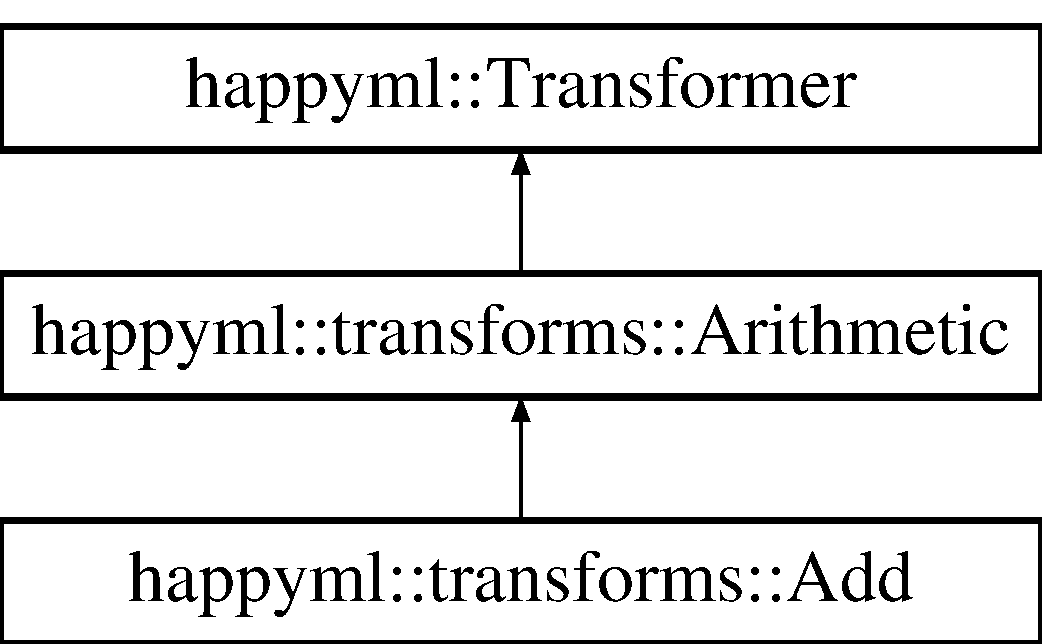
\includegraphics[height=3.000000cm]{classhappyml_1_1transforms_1_1Add}
\end{center}
\end{figure}
\subsection*{Public Member Functions}
\begin{DoxyCompactItemize}
\item 
\hyperlink{classhappyml_1_1transforms_1_1Add_a5114a7acadd81212909f9fa5bce382e6}{Add} (int f, double p, bool nf=false)
\item 
void \hyperlink{classhappyml_1_1transforms_1_1Add_a42a12de9fefcdb7b4c3c669f8d023a2f}{apply} (mat \&x, int col) const 
\end{DoxyCompactItemize}
\subsection*{Additional Inherited Members}


\subsection{Constructor \& Destructor Documentation}
\index{happyml\+::transforms\+::\+Add@{happyml\+::transforms\+::\+Add}!Add@{Add}}
\index{Add@{Add}!happyml\+::transforms\+::\+Add@{happyml\+::transforms\+::\+Add}}
\subsubsection[{\texorpdfstring{Add(int f, double p, bool nf=false)}{Add(int f, double p, bool nf=false)}}]{\setlength{\rightskip}{0pt plus 5cm}happyml\+::transforms\+::\+Add\+::\+Add (
\begin{DoxyParamCaption}
\item[{int}]{f, }
\item[{double}]{p, }
\item[{bool}]{nf = {\ttfamily false}}
\end{DoxyParamCaption}
)\hspace{0.3cm}{\ttfamily [inline]}}\hypertarget{classhappyml_1_1transforms_1_1Add_a5114a7acadd81212909f9fa5bce382e6}{}\label{classhappyml_1_1transforms_1_1Add_a5114a7acadd81212909f9fa5bce382e6}


\subsection{Member Function Documentation}
\index{happyml\+::transforms\+::\+Add@{happyml\+::transforms\+::\+Add}!apply@{apply}}
\index{apply@{apply}!happyml\+::transforms\+::\+Add@{happyml\+::transforms\+::\+Add}}
\subsubsection[{\texorpdfstring{apply(mat \&x, int col) const }{apply(mat &x, int col) const }}]{\setlength{\rightskip}{0pt plus 5cm}void happyml\+::transforms\+::\+Add\+::apply (
\begin{DoxyParamCaption}
\item[{mat \&}]{x, }
\item[{int}]{col}
\end{DoxyParamCaption}
) const\hspace{0.3cm}{\ttfamily [virtual]}}\hypertarget{classhappyml_1_1transforms_1_1Add_a42a12de9fefcdb7b4c3c669f8d023a2f}{}\label{classhappyml_1_1transforms_1_1Add_a42a12de9fefcdb7b4c3c669f8d023a2f}


Implements \hyperlink{classhappyml_1_1transforms_1_1Arithmetic_a85191dcd8734e18424b92b870d7b9d73}{happyml\+::transforms\+::\+Arithmetic}.



The documentation for this class was generated from the following files\+:\begin{DoxyCompactItemize}
\item 
include/happyml/transformers/\hyperlink{transformer_8h}{transformer.\+h}\item 
src/transformers/\hyperlink{transformer_8cpp}{transformer.\+cpp}\end{DoxyCompactItemize}

\hypertarget{classhappyml_1_1transforms_1_1Arithmetic}{}\section{happyml\+:\+:transforms\+:\+:Arithmetic Class Reference}
\label{classhappyml_1_1transforms_1_1Arithmetic}\index{happyml\+::transforms\+::\+Arithmetic@{happyml\+::transforms\+::\+Arithmetic}}


{\ttfamily \#include $<$transformer.\+h$>$}

Inheritance diagram for happyml\+:\+:transforms\+:\+:Arithmetic\+:\begin{figure}[H]
\begin{center}
\leavevmode
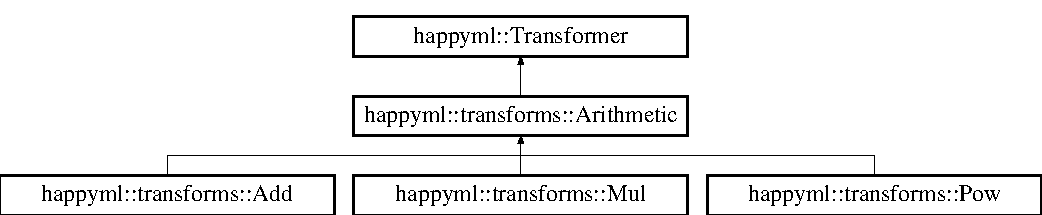
\includegraphics[height=2.886598cm]{classhappyml_1_1transforms_1_1Arithmetic}
\end{center}
\end{figure}
\subsection*{Public Member Functions}
\begin{DoxyCompactItemize}
\item 
\hyperlink{classhappyml_1_1transforms_1_1Arithmetic_a0a57820a202d232af4527a2bb4ecf67a}{Arithmetic} (int f, double p, bool nf)
\item 
void \hyperlink{classhappyml_1_1transforms_1_1Arithmetic_aafe6e2ef231e5515f2068b8340aac93a}{apply} (\hyperlink{classhappyml_1_1DataSet}{Data\+Set} \&dataset) const 
\begin{DoxyCompactList}\small\item\em Applies all the transformations at the given dataset. \end{DoxyCompactList}\item 
\hyperlink{namespacehappyml_a03602d1ec49393790b8a0449f40cd01f}{Input} \hyperlink{classhappyml_1_1transforms_1_1Arithmetic_ac32e38e089435dc407bc9b7a338bc845}{apply} (const \hyperlink{namespacehappyml_a03602d1ec49393790b8a0449f40cd01f}{Input} \&input) const 
\begin{DoxyCompactList}\small\item\em Applies all the transformations at the given input. \end{DoxyCompactList}\item 
virtual void \hyperlink{classhappyml_1_1transforms_1_1Arithmetic_a85191dcd8734e18424b92b870d7b9d73}{apply} (mat \&x, int col) const  =0
\end{DoxyCompactItemize}
\subsection*{Protected Attributes}
\begin{DoxyCompactItemize}
\item 
double \hyperlink{classhappyml_1_1transforms_1_1Arithmetic_a64c5ee9c6775b2f19799eeae75c37ea1}{param}
\item 
int \hyperlink{classhappyml_1_1transforms_1_1Arithmetic_a9f9d1fe8c2fbae1fccce0d5d230406b1}{feature}
\item 
bool \hyperlink{classhappyml_1_1transforms_1_1Arithmetic_a05e8518ae4bf508f3a572de827f42316}{new\+Feature}
\end{DoxyCompactItemize}


\subsection{Constructor \& Destructor Documentation}
\index{happyml\+::transforms\+::\+Arithmetic@{happyml\+::transforms\+::\+Arithmetic}!Arithmetic@{Arithmetic}}
\index{Arithmetic@{Arithmetic}!happyml\+::transforms\+::\+Arithmetic@{happyml\+::transforms\+::\+Arithmetic}}
\subsubsection[{\texorpdfstring{Arithmetic(int f, double p, bool nf)}{Arithmetic(int f, double p, bool nf)}}]{\setlength{\rightskip}{0pt plus 5cm}happyml\+::transforms\+::\+Arithmetic\+::\+Arithmetic (
\begin{DoxyParamCaption}
\item[{int}]{f, }
\item[{double}]{p, }
\item[{bool}]{nf}
\end{DoxyParamCaption}
)\hspace{0.3cm}{\ttfamily [inline]}}\hypertarget{classhappyml_1_1transforms_1_1Arithmetic_a0a57820a202d232af4527a2bb4ecf67a}{}\label{classhappyml_1_1transforms_1_1Arithmetic_a0a57820a202d232af4527a2bb4ecf67a}


\subsection{Member Function Documentation}
\index{happyml\+::transforms\+::\+Arithmetic@{happyml\+::transforms\+::\+Arithmetic}!apply@{apply}}
\index{apply@{apply}!happyml\+::transforms\+::\+Arithmetic@{happyml\+::transforms\+::\+Arithmetic}}
\subsubsection[{\texorpdfstring{apply(\+Data\+Set \&dataset) const }{apply(DataSet &dataset) const }}]{\setlength{\rightskip}{0pt plus 5cm}void happyml\+::transforms\+::\+Arithmetic\+::apply (
\begin{DoxyParamCaption}
\item[{{\bf Data\+Set} \&}]{dataset}
\end{DoxyParamCaption}
) const\hspace{0.3cm}{\ttfamily [virtual]}}\hypertarget{classhappyml_1_1transforms_1_1Arithmetic_aafe6e2ef231e5515f2068b8340aac93a}{}\label{classhappyml_1_1transforms_1_1Arithmetic_aafe6e2ef231e5515f2068b8340aac93a}


Applies all the transformations at the given dataset. 


\begin{DoxyParams}{Parameters}
{\em dataset} & Dataset to transform. \\
\hline
\end{DoxyParams}


Reimplemented from \hyperlink{classhappyml_1_1Transformer_a169a2a8434124c1dd8e671bca2cfa71d}{happyml\+::\+Transformer}.

\index{happyml\+::transforms\+::\+Arithmetic@{happyml\+::transforms\+::\+Arithmetic}!apply@{apply}}
\index{apply@{apply}!happyml\+::transforms\+::\+Arithmetic@{happyml\+::transforms\+::\+Arithmetic}}
\subsubsection[{\texorpdfstring{apply(const Input \&input) const }{apply(const Input &input) const }}]{\setlength{\rightskip}{0pt plus 5cm}{\bf Input} happyml\+::transforms\+::\+Arithmetic\+::apply (
\begin{DoxyParamCaption}
\item[{const {\bf Input} \&}]{input}
\end{DoxyParamCaption}
) const\hspace{0.3cm}{\ttfamily [virtual]}}\hypertarget{classhappyml_1_1transforms_1_1Arithmetic_ac32e38e089435dc407bc9b7a338bc845}{}\label{classhappyml_1_1transforms_1_1Arithmetic_ac32e38e089435dc407bc9b7a338bc845}


Applies all the transformations at the given input. 


\begin{DoxyParams}{Parameters}
{\em input} & Input to transform.\\
\hline
\end{DoxyParams}
\begin{DoxyReturn}{Returns}
A transformated version of the input. 
\end{DoxyReturn}


Reimplemented from \hyperlink{classhappyml_1_1Transformer_a3e0eb67990c90c461466307fdefab45c}{happyml\+::\+Transformer}.

\index{happyml\+::transforms\+::\+Arithmetic@{happyml\+::transforms\+::\+Arithmetic}!apply@{apply}}
\index{apply@{apply}!happyml\+::transforms\+::\+Arithmetic@{happyml\+::transforms\+::\+Arithmetic}}
\subsubsection[{\texorpdfstring{apply(mat \&x, int col) const  =0}{apply(mat &x, int col) const  =0}}]{\setlength{\rightskip}{0pt plus 5cm}virtual void happyml\+::transforms\+::\+Arithmetic\+::apply (
\begin{DoxyParamCaption}
\item[{mat \&}]{x, }
\item[{int}]{col}
\end{DoxyParamCaption}
) const\hspace{0.3cm}{\ttfamily [pure virtual]}}\hypertarget{classhappyml_1_1transforms_1_1Arithmetic_a85191dcd8734e18424b92b870d7b9d73}{}\label{classhappyml_1_1transforms_1_1Arithmetic_a85191dcd8734e18424b92b870d7b9d73}


Implemented in \hyperlink{classhappyml_1_1transforms_1_1Mul_afc91c3f53e31af40b314cc0d9d5552fa}{happyml\+::transforms\+::\+Mul}, \hyperlink{classhappyml_1_1transforms_1_1Add_a42a12de9fefcdb7b4c3c669f8d023a2f}{happyml\+::transforms\+::\+Add}, and \hyperlink{classhappyml_1_1transforms_1_1Pow_af6d691fc3afbff2ee8f85db1725c2ea8}{happyml\+::transforms\+::\+Pow}.



\subsection{Member Data Documentation}
\index{happyml\+::transforms\+::\+Arithmetic@{happyml\+::transforms\+::\+Arithmetic}!feature@{feature}}
\index{feature@{feature}!happyml\+::transforms\+::\+Arithmetic@{happyml\+::transforms\+::\+Arithmetic}}
\subsubsection[{\texorpdfstring{feature}{feature}}]{\setlength{\rightskip}{0pt plus 5cm}int happyml\+::transforms\+::\+Arithmetic\+::feature\hspace{0.3cm}{\ttfamily [protected]}}\hypertarget{classhappyml_1_1transforms_1_1Arithmetic_a9f9d1fe8c2fbae1fccce0d5d230406b1}{}\label{classhappyml_1_1transforms_1_1Arithmetic_a9f9d1fe8c2fbae1fccce0d5d230406b1}
\index{happyml\+::transforms\+::\+Arithmetic@{happyml\+::transforms\+::\+Arithmetic}!new\+Feature@{new\+Feature}}
\index{new\+Feature@{new\+Feature}!happyml\+::transforms\+::\+Arithmetic@{happyml\+::transforms\+::\+Arithmetic}}
\subsubsection[{\texorpdfstring{new\+Feature}{newFeature}}]{\setlength{\rightskip}{0pt plus 5cm}bool happyml\+::transforms\+::\+Arithmetic\+::new\+Feature\hspace{0.3cm}{\ttfamily [protected]}}\hypertarget{classhappyml_1_1transforms_1_1Arithmetic_a05e8518ae4bf508f3a572de827f42316}{}\label{classhappyml_1_1transforms_1_1Arithmetic_a05e8518ae4bf508f3a572de827f42316}
\index{happyml\+::transforms\+::\+Arithmetic@{happyml\+::transforms\+::\+Arithmetic}!param@{param}}
\index{param@{param}!happyml\+::transforms\+::\+Arithmetic@{happyml\+::transforms\+::\+Arithmetic}}
\subsubsection[{\texorpdfstring{param}{param}}]{\setlength{\rightskip}{0pt plus 5cm}double happyml\+::transforms\+::\+Arithmetic\+::param\hspace{0.3cm}{\ttfamily [protected]}}\hypertarget{classhappyml_1_1transforms_1_1Arithmetic_a64c5ee9c6775b2f19799eeae75c37ea1}{}\label{classhappyml_1_1transforms_1_1Arithmetic_a64c5ee9c6775b2f19799eeae75c37ea1}


The documentation for this class was generated from the following files\+:\begin{DoxyCompactItemize}
\item 
include/happyml/transformers/\hyperlink{transformer_8h}{transformer.\+h}\item 
src/transformers/\hyperlink{transformer_8cpp}{transformer.\+cpp}\end{DoxyCompactItemize}

\hypertarget{classhappyml_1_1Classifier}{}\section{happyml\+:\+:Classifier Class Reference}
\label{classhappyml_1_1Classifier}\index{happyml\+::\+Classifier@{happyml\+::\+Classifier}}


Abstract class that represent an algorithm that classifies an input in classes.  




{\ttfamily \#include $<$predictor.\+h$>$}

Inheritance diagram for happyml\+:\+:Classifier\+:\begin{figure}[H]
\begin{center}
\leavevmode
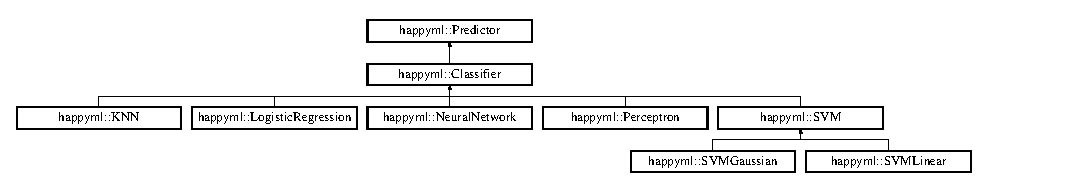
\includegraphics[height=2.085661cm]{classhappyml_1_1Classifier}
\end{center}
\end{figure}
\subsection*{Public Member Functions}
\begin{DoxyCompactItemize}
\item 
virtual double \hyperlink{classhappyml_1_1Classifier_ac72f1b0b689aaff5078978ae198318df}{error} (const \hyperlink{namespacehappyml_a03602d1ec49393790b8a0449f40cd01f}{Input} \&x, double y) const 
\begin{DoxyCompactList}\small\item\em Compute the error of the classifier in a given input. \end{DoxyCompactList}\end{DoxyCompactItemize}


\subsection{Detailed Description}
Abstract class that represent an algorithm that classifies an input in classes. 

\subsection{Member Function Documentation}
\index{happyml\+::\+Classifier@{happyml\+::\+Classifier}!error@{error}}
\index{error@{error}!happyml\+::\+Classifier@{happyml\+::\+Classifier}}
\subsubsection[{\texorpdfstring{error(const Input \&x, double y) const }{error(const Input &x, double y) const }}]{\setlength{\rightskip}{0pt plus 5cm}double happyml\+::\+Classifier\+::error (
\begin{DoxyParamCaption}
\item[{const {\bf Input} \&}]{x, }
\item[{double}]{y}
\end{DoxyParamCaption}
) const\hspace{0.3cm}{\ttfamily [virtual]}}\hypertarget{classhappyml_1_1Classifier_ac72f1b0b689aaff5078978ae198318df}{}\label{classhappyml_1_1Classifier_ac72f1b0b689aaff5078978ae198318df}


Compute the error of the classifier in a given input. 

By default it computes the binary error.


\begin{DoxyParams}{Parameters}
{\em x} & The input vector. \\
\hline
{\em y} & Correct output.\\
\hline
\end{DoxyParams}
\begin{DoxyReturn}{Returns}
0 if x is correctly predicted or 1 if not. 
\end{DoxyReturn}


Reimplemented from \hyperlink{classhappyml_1_1Predictor_aeb20c07843cf4a2b7df76b2f0d0e0b13}{happyml\+::\+Predictor}.



The documentation for this class was generated from the following files\+:\begin{DoxyCompactItemize}
\item 
include/happyml/\hyperlink{predictor_8h}{predictor.\+h}\item 
src/\hyperlink{predictor_8cpp}{predictor.\+cpp}\end{DoxyCompactItemize}

\hypertarget{classhappyml_1_1DataSet}{}\section{happyml\+:\+:Data\+Set Class Reference}
\label{classhappyml_1_1DataSet}\index{happyml\+::\+Data\+Set@{happyml\+::\+Data\+Set}}


Generic collection of inputs and outputs.  




{\ttfamily \#include $<$dataset.\+h$>$}

Inheritance diagram for happyml\+:\+:Data\+Set\+:\begin{figure}[H]
\begin{center}
\leavevmode
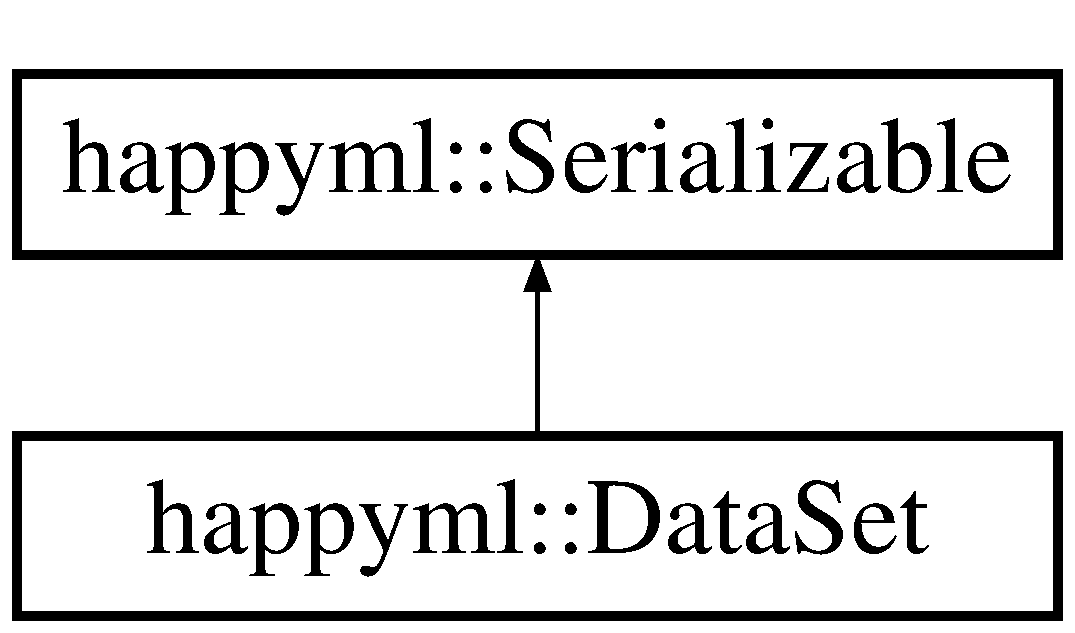
\includegraphics[height=2.000000cm]{classhappyml_1_1DataSet}
\end{center}
\end{figure}
\subsection*{Public Member Functions}
\begin{DoxyCompactItemize}
\item 
\hyperlink{classhappyml_1_1DataSet_a49c36517dc2ab29e2c20ba83e9c8a5ea}{Data\+Set} (unsigned dim=0, unsigned size=0, unsigned outputs=1)
\begin{DoxyCompactList}\small\item\em Creates a generic collection of inputs and outputs. \end{DoxyCompactList}\item 
void \hyperlink{classhappyml_1_1DataSet_aa2e2f9c87aefbf9c7a2b8793f197b828}{read} (istream \&stream)
\begin{DoxyCompactList}\small\item\em Creates a dataset from a text input stream with the following format\+: \end{DoxyCompactList}\item 
void \hyperlink{classhappyml_1_1DataSet_aeab3657e98d735fef9af63cd416f095a}{read} (istream \&stream, int n\+\_\+outputs)
\item 
void \hyperlink{classhappyml_1_1DataSet_a5cc37a7dae6c1757ee93dee1f95e91a6}{load} (const string \&filename, int n\+\_\+outputs)
\item 
void \hyperlink{classhappyml_1_1DataSet_ae1f10ba937cdf97e7ce6046c55a9a665}{load} (const string \&filename, bool one\+\_\+hot)
\item 
void \hyperlink{classhappyml_1_1DataSet_a1bed7d89826c5b9fb23c3e2d0f690b22}{write} (ostream \&stream) const 
\begin{DoxyCompactList}\small\item\em Write to an output stream the next data\+: \end{DoxyCompactList}\item 
void \hyperlink{classhappyml_1_1DataSet_a8706653aeaef403a278f178e4aa38f75}{shuffle} ()
\item 
void \hyperlink{classhappyml_1_1DataSet_a5ec56f6731cb4ef784936844b6409198}{reduce} (int)
\item 
void \hyperlink{classhappyml_1_1DataSet_ab56a70830be900d8a9b4e8f90f5c615a}{noise} (int)
\end{DoxyCompactItemize}
\subsection*{Public Attributes}
\begin{DoxyCompactItemize}
\item 
unsigned \hyperlink{classhappyml_1_1DataSet_a0a154016e91e970cdd700e110f1cae80}{d}
\begin{DoxyCompactList}\small\item\em Dimension of the inputs vectors of this dataset ( $d$). \end{DoxyCompactList}\item 
unsigned \hyperlink{classhappyml_1_1DataSet_a18457530136087ab5e09e96125655ab5}{N}
\begin{DoxyCompactList}\small\item\em Number of pairs $(\mathbf{x}, y)$ in the dataset. \end{DoxyCompactList}\item 
unsigned \hyperlink{classhappyml_1_1DataSet_a23743c9bd5463966207e1199eba0c9d2}{k}
\begin{DoxyCompactList}\small\item\em Number of outputs by sample. \end{DoxyCompactList}\item 
mat \hyperlink{classhappyml_1_1DataSet_a692f8bd10b94c74df7e7f9010c78820a}{X}
\begin{DoxyCompactList}\small\item\em Matrix with all the inputs. \end{DoxyCompactList}\item 
mat \hyperlink{classhappyml_1_1DataSet_ac75419fb46abcc2841226a8441674d48}{y}
\begin{DoxyCompactList}\small\item\em Expected outputs. \end{DoxyCompactList}\end{DoxyCompactItemize}


\subsection{Detailed Description}
Generic collection of inputs and outputs. 

We denote it with $\mathcal{D}$. 

\subsection{Constructor \& Destructor Documentation}
\index{happyml\+::\+Data\+Set@{happyml\+::\+Data\+Set}!Data\+Set@{Data\+Set}}
\index{Data\+Set@{Data\+Set}!happyml\+::\+Data\+Set@{happyml\+::\+Data\+Set}}
\subsubsection[{\texorpdfstring{Data\+Set(unsigned dim=0, unsigned size=0, unsigned outputs=1)}{DataSet(unsigned dim=0, unsigned size=0, unsigned outputs=1)}}]{\setlength{\rightskip}{0pt plus 5cm}happyml\+::\+Data\+Set\+::\+Data\+Set (
\begin{DoxyParamCaption}
\item[{unsigned}]{dim = {\ttfamily 0}, }
\item[{unsigned}]{size = {\ttfamily 0}, }
\item[{unsigned}]{outputs = {\ttfamily 1}}
\end{DoxyParamCaption}
)\hspace{0.3cm}{\ttfamily [inline]}}\hypertarget{classhappyml_1_1DataSet_a49c36517dc2ab29e2c20ba83e9c8a5ea}{}\label{classhappyml_1_1DataSet_a49c36517dc2ab29e2c20ba83e9c8a5ea}


Creates a generic collection of inputs and outputs. 


\begin{DoxyParams}{Parameters}
{\em dim} & Dimension $d$ of the inputs. \\
\hline
{\em size} & Number of inputs ( $N$) in the dataset. \\
\hline
{\em output} & Number of tail columns to be used \\
\hline
\end{DoxyParams}


\subsection{Member Function Documentation}
\index{happyml\+::\+Data\+Set@{happyml\+::\+Data\+Set}!load@{load}}
\index{load@{load}!happyml\+::\+Data\+Set@{happyml\+::\+Data\+Set}}
\subsubsection[{\texorpdfstring{load(const string \&filename, int n\+\_\+outputs)}{load(const string &filename, int n_outputs)}}]{\setlength{\rightskip}{0pt plus 5cm}void happyml\+::\+Data\+Set\+::load (
\begin{DoxyParamCaption}
\item[{const string \&}]{filename, }
\item[{int}]{n\+\_\+outputs}
\end{DoxyParamCaption}
)}\hypertarget{classhappyml_1_1DataSet_a5cc37a7dae6c1757ee93dee1f95e91a6}{}\label{classhappyml_1_1DataSet_a5cc37a7dae6c1757ee93dee1f95e91a6}
\index{happyml\+::\+Data\+Set@{happyml\+::\+Data\+Set}!load@{load}}
\index{load@{load}!happyml\+::\+Data\+Set@{happyml\+::\+Data\+Set}}
\subsubsection[{\texorpdfstring{load(const string \&filename, bool one\+\_\+hot)}{load(const string &filename, bool one_hot)}}]{\setlength{\rightskip}{0pt plus 5cm}void happyml\+::\+Data\+Set\+::load (
\begin{DoxyParamCaption}
\item[{const string \&}]{filename, }
\item[{bool}]{one\+\_\+hot}
\end{DoxyParamCaption}
)}\hypertarget{classhappyml_1_1DataSet_ae1f10ba937cdf97e7ce6046c55a9a665}{}\label{classhappyml_1_1DataSet_ae1f10ba937cdf97e7ce6046c55a9a665}
\index{happyml\+::\+Data\+Set@{happyml\+::\+Data\+Set}!noise@{noise}}
\index{noise@{noise}!happyml\+::\+Data\+Set@{happyml\+::\+Data\+Set}}
\subsubsection[{\texorpdfstring{noise(int)}{noise(int)}}]{\setlength{\rightskip}{0pt plus 5cm}void happyml\+::\+Data\+Set\+::noise (
\begin{DoxyParamCaption}
\item[{int}]{n}
\end{DoxyParamCaption}
)}\hypertarget{classhappyml_1_1DataSet_ab56a70830be900d8a9b4e8f90f5c615a}{}\label{classhappyml_1_1DataSet_ab56a70830be900d8a9b4e8f90f5c615a}
\index{happyml\+::\+Data\+Set@{happyml\+::\+Data\+Set}!read@{read}}
\index{read@{read}!happyml\+::\+Data\+Set@{happyml\+::\+Data\+Set}}
\subsubsection[{\texorpdfstring{read(istream \&stream)}{read(istream &stream)}}]{\setlength{\rightskip}{0pt plus 5cm}void happyml\+::\+Data\+Set\+::read (
\begin{DoxyParamCaption}
\item[{istream \&}]{stream}
\end{DoxyParamCaption}
)\hspace{0.3cm}{\ttfamily [virtual]}}\hypertarget{classhappyml_1_1DataSet_aa2e2f9c87aefbf9c7a2b8793f197b828}{}\label{classhappyml_1_1DataSet_aa2e2f9c87aefbf9c7a2b8793f197b828}


Creates a dataset from a text input stream with the following format\+: 

$\\ x_{01},x_{02},\cdots,x_{0d},y_{0}\\ x_{11},x_{12},\cdots,x_{1d},y_{1}\\ \ \ \vdots\ \ ,\ \ \vdots\ \ ,\ \cdots\ ,\ \ \vdots\ \ ,\ \ \vdots\\ x_{(N-1)1},x_{(N-1)2},\cdots,x_{(N-1)d},y_{(N-1)} $ 

Implements \hyperlink{classhappyml_1_1Serializable_aef5c211d8e9c1c425b33c657824c2f0c}{happyml\+::\+Serializable}.

\index{happyml\+::\+Data\+Set@{happyml\+::\+Data\+Set}!read@{read}}
\index{read@{read}!happyml\+::\+Data\+Set@{happyml\+::\+Data\+Set}}
\subsubsection[{\texorpdfstring{read(istream \&stream, int n\+\_\+outputs)}{read(istream &stream, int n_outputs)}}]{\setlength{\rightskip}{0pt plus 5cm}void happyml\+::\+Data\+Set\+::read (
\begin{DoxyParamCaption}
\item[{istream \&}]{stream, }
\item[{int}]{n\+\_\+outputs}
\end{DoxyParamCaption}
)}\hypertarget{classhappyml_1_1DataSet_aeab3657e98d735fef9af63cd416f095a}{}\label{classhappyml_1_1DataSet_aeab3657e98d735fef9af63cd416f095a}
\index{happyml\+::\+Data\+Set@{happyml\+::\+Data\+Set}!reduce@{reduce}}
\index{reduce@{reduce}!happyml\+::\+Data\+Set@{happyml\+::\+Data\+Set}}
\subsubsection[{\texorpdfstring{reduce(int)}{reduce(int)}}]{\setlength{\rightskip}{0pt plus 5cm}void happyml\+::\+Data\+Set\+::reduce (
\begin{DoxyParamCaption}
\item[{int}]{n}
\end{DoxyParamCaption}
)}\hypertarget{classhappyml_1_1DataSet_a5ec56f6731cb4ef784936844b6409198}{}\label{classhappyml_1_1DataSet_a5ec56f6731cb4ef784936844b6409198}
\index{happyml\+::\+Data\+Set@{happyml\+::\+Data\+Set}!shuffle@{shuffle}}
\index{shuffle@{shuffle}!happyml\+::\+Data\+Set@{happyml\+::\+Data\+Set}}
\subsubsection[{\texorpdfstring{shuffle()}{shuffle()}}]{\setlength{\rightskip}{0pt plus 5cm}void happyml\+::\+Data\+Set\+::shuffle (
\begin{DoxyParamCaption}
{}
\end{DoxyParamCaption}
)}\hypertarget{classhappyml_1_1DataSet_a8706653aeaef403a278f178e4aa38f75}{}\label{classhappyml_1_1DataSet_a8706653aeaef403a278f178e4aa38f75}
\index{happyml\+::\+Data\+Set@{happyml\+::\+Data\+Set}!write@{write}}
\index{write@{write}!happyml\+::\+Data\+Set@{happyml\+::\+Data\+Set}}
\subsubsection[{\texorpdfstring{write(ostream \&stream) const }{write(ostream &stream) const }}]{\setlength{\rightskip}{0pt plus 5cm}void happyml\+::\+Data\+Set\+::write (
\begin{DoxyParamCaption}
\item[{ostream \&}]{stream}
\end{DoxyParamCaption}
) const\hspace{0.3cm}{\ttfamily [virtual]}}\hypertarget{classhappyml_1_1DataSet_a1bed7d89826c5b9fb23c3e2d0f690b22}{}\label{classhappyml_1_1DataSet_a1bed7d89826c5b9fb23c3e2d0f690b22}


Write to an output stream the next data\+: 

$\\ x_{01},x_{02},\cdots,x_{0d},y_{0}\\ x_{11},x_{12},\cdots,x_{1d},y_{1}\\ \ \ \vdots\ \ ,\ \ \vdots\ \ ,\ \cdots\ ,\ \ \vdots\ \ ,\ \ \vdots\\ x_{(N-1)1},x_{(N-1)2},\cdots,x_{(N-1)d},y_{(N-1)} $ 

Implements \hyperlink{classhappyml_1_1Serializable_a2d503e4c2e39c5be8a33bcc8b691949f}{happyml\+::\+Serializable}.



\subsection{Member Data Documentation}
\index{happyml\+::\+Data\+Set@{happyml\+::\+Data\+Set}!d@{d}}
\index{d@{d}!happyml\+::\+Data\+Set@{happyml\+::\+Data\+Set}}
\subsubsection[{\texorpdfstring{d}{d}}]{\setlength{\rightskip}{0pt plus 5cm}unsigned happyml\+::\+Data\+Set\+::d}\hypertarget{classhappyml_1_1DataSet_a0a154016e91e970cdd700e110f1cae80}{}\label{classhappyml_1_1DataSet_a0a154016e91e970cdd700e110f1cae80}


Dimension of the inputs vectors of this dataset ( $d$). 

All the points has the same dimension. \index{happyml\+::\+Data\+Set@{happyml\+::\+Data\+Set}!k@{k}}
\index{k@{k}!happyml\+::\+Data\+Set@{happyml\+::\+Data\+Set}}
\subsubsection[{\texorpdfstring{k}{k}}]{\setlength{\rightskip}{0pt plus 5cm}unsigned happyml\+::\+Data\+Set\+::k}\hypertarget{classhappyml_1_1DataSet_a23743c9bd5463966207e1199eba0c9d2}{}\label{classhappyml_1_1DataSet_a23743c9bd5463966207e1199eba0c9d2}


Number of outputs by sample. 

\index{happyml\+::\+Data\+Set@{happyml\+::\+Data\+Set}!N@{N}}
\index{N@{N}!happyml\+::\+Data\+Set@{happyml\+::\+Data\+Set}}
\subsubsection[{\texorpdfstring{N}{N}}]{\setlength{\rightskip}{0pt plus 5cm}unsigned happyml\+::\+Data\+Set\+::N}\hypertarget{classhappyml_1_1DataSet_a18457530136087ab5e09e96125655ab5}{}\label{classhappyml_1_1DataSet_a18457530136087ab5e09e96125655ab5}


Number of pairs $(\mathbf{x}, y)$ in the dataset. 

We denote it with $N$. \index{happyml\+::\+Data\+Set@{happyml\+::\+Data\+Set}!X@{X}}
\index{X@{X}!happyml\+::\+Data\+Set@{happyml\+::\+Data\+Set}}
\subsubsection[{\texorpdfstring{X}{X}}]{\setlength{\rightskip}{0pt plus 5cm}mat happyml\+::\+Data\+Set\+::X}\hypertarget{classhappyml_1_1DataSet_a692f8bd10b94c74df7e7f9010c78820a}{}\label{classhappyml_1_1DataSet_a692f8bd10b94c74df7e7f9010c78820a}


Matrix with all the inputs. 

$ \mathbf{X} = \begin{pmatrix} \mathbf{x}^{\rm T}_0 \\ \mathbf{x}^{\rm T}_1 \\ \vdots \\ \mathbf{x}^{\rm T}_{N - 1} \end{pmatrix} = \begin{pmatrix} x_{00} & \cdots & x_{0d} \\ x_{10} & \cdots & x_{1d} \\ \vdots & \ddots & \vdots \\ x_{(N-1)0} & \cdots & x_{(N-1)d} \end{pmatrix} $ \index{happyml\+::\+Data\+Set@{happyml\+::\+Data\+Set}!y@{y}}
\index{y@{y}!happyml\+::\+Data\+Set@{happyml\+::\+Data\+Set}}
\subsubsection[{\texorpdfstring{y}{y}}]{\setlength{\rightskip}{0pt plus 5cm}mat happyml\+::\+Data\+Set\+::y}\hypertarget{classhappyml_1_1DataSet_ac75419fb46abcc2841226a8441674d48}{}\label{classhappyml_1_1DataSet_ac75419fb46abcc2841226a8441674d48}


Expected outputs. 

$ \mathbf{y} = \begin{pmatrix} y_0 \\ y_1 \\ \vdots \\ y_{N - 1} \end{pmatrix} $ 

The documentation for this class was generated from the following files\+:\begin{DoxyCompactItemize}
\item 
include/happyml/\hyperlink{dataset_8h}{dataset.\+h}\item 
src/\hyperlink{dataset_8cpp}{dataset.\+cpp}\end{DoxyCompactItemize}

\hypertarget{classhappyml_1_1Denormalizer}{}\section{happyml\+:\+:Denormalizer Class Reference}
\label{classhappyml_1_1Denormalizer}\index{happyml\+::\+Denormalizer@{happyml\+::\+Denormalizer}}


{\ttfamily \#include $<$normalizer.\+h$>$}

Inheritance diagram for happyml\+:\+:Denormalizer\+:\begin{figure}[H]
\begin{center}
\leavevmode
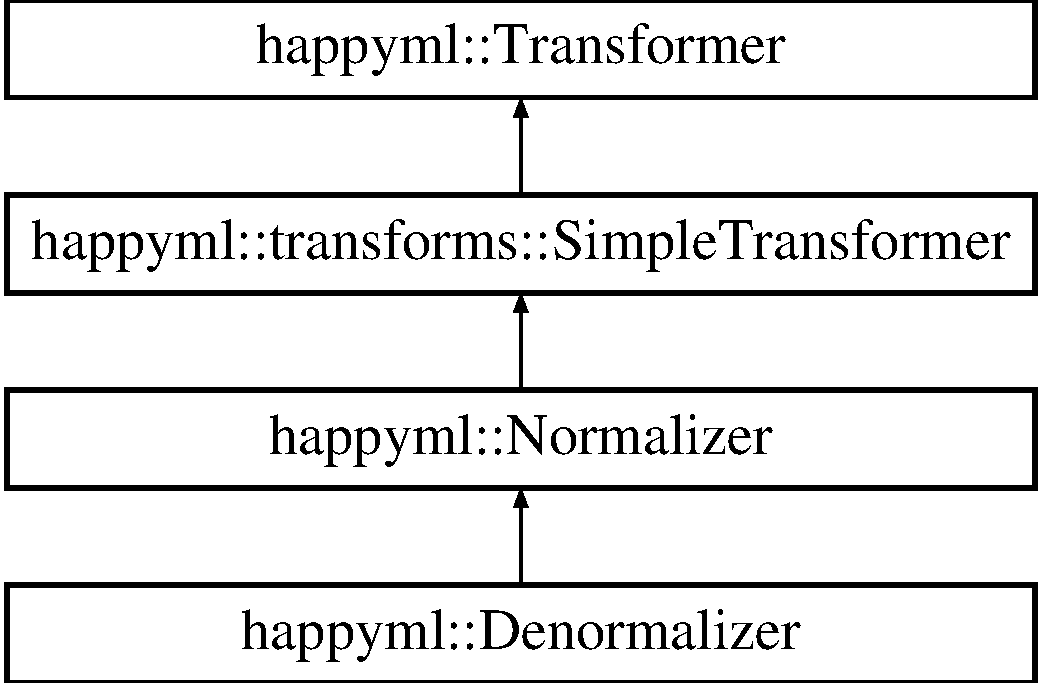
\includegraphics[height=4.000000cm]{classhappyml_1_1Denormalizer}
\end{center}
\end{figure}
\subsection*{Public Member Functions}
\begin{DoxyCompactItemize}
\item 
\hyperlink{classhappyml_1_1Denormalizer_a3afa7cfb90125b5ff82bc8b7265287fc}{Denormalizer} (const \hyperlink{classhappyml_1_1DataSet}{Data\+Set} \&dataset)
\begin{DoxyCompactList}\small\item\em Creates a denormalizer that will use min and max data obtained from the dataset. \end{DoxyCompactList}\item 
\hyperlink{classhappyml_1_1Denormalizer_afdb1825e2e4c813db0555ca70c3d745a}{Denormalizer} (const mat \&x)
\begin{DoxyCompactList}\small\item\em Creates a denormalizer that will use min and max data obtained from the matrix x. \end{DoxyCompactList}\item 
\hyperlink{classhappyml_1_1Denormalizer_ad0cfa938971d2ddeccdf7c2723feb698}{Denormalizer} (const vec \&minvec, const vec \&maxvec)
\begin{DoxyCompactList}\small\item\em Creates a denormalizer that will use min and max data obtained from the dataset. \end{DoxyCompactList}\item 
\hyperlink{classhappyml_1_1Denormalizer_a6b8296bc74b7c90b8237a596da893d2d}{Denormalizer} (const \hyperlink{classhappyml_1_1Normalizer}{Normalizer} \&n)
\begin{DoxyCompactList}\small\item\em Creates a denormalizer using the given normalizer. \end{DoxyCompactList}\item 
\hyperlink{classhappyml_1_1Denormalizer_ad0fa1ca5cf1296d1a383ad617cfe82b5}{$\sim$\+Denormalizer} ()
\item 
virtual void \hyperlink{classhappyml_1_1Denormalizer_a2f1aa35006d0573f07fc33e8f154c170}{apply} (mat \&x) const 
\end{DoxyCompactItemize}
\subsection*{Additional Inherited Members}


\subsection{Constructor \& Destructor Documentation}
\index{happyml\+::\+Denormalizer@{happyml\+::\+Denormalizer}!Denormalizer@{Denormalizer}}
\index{Denormalizer@{Denormalizer}!happyml\+::\+Denormalizer@{happyml\+::\+Denormalizer}}
\subsubsection[{\texorpdfstring{Denormalizer(const Data\+Set \&dataset)}{Denormalizer(const DataSet &dataset)}}]{\setlength{\rightskip}{0pt plus 5cm}happyml\+::\+Denormalizer\+::\+Denormalizer (
\begin{DoxyParamCaption}
\item[{const {\bf Data\+Set} \&}]{dataset}
\end{DoxyParamCaption}
)\hspace{0.3cm}{\ttfamily [inline]}}\hypertarget{classhappyml_1_1Denormalizer_a3afa7cfb90125b5ff82bc8b7265287fc}{}\label{classhappyml_1_1Denormalizer_a3afa7cfb90125b5ff82bc8b7265287fc}


Creates a denormalizer that will use min and max data obtained from the dataset. 


\begin{DoxyParams}{Parameters}
{\em dataset} & Dataset from which it will be extracted the min and max that will be use when apply denormalization. \\
\hline
\end{DoxyParams}
\index{happyml\+::\+Denormalizer@{happyml\+::\+Denormalizer}!Denormalizer@{Denormalizer}}
\index{Denormalizer@{Denormalizer}!happyml\+::\+Denormalizer@{happyml\+::\+Denormalizer}}
\subsubsection[{\texorpdfstring{Denormalizer(const mat \&x)}{Denormalizer(const mat &x)}}]{\setlength{\rightskip}{0pt plus 5cm}happyml\+::\+Denormalizer\+::\+Denormalizer (
\begin{DoxyParamCaption}
\item[{const mat \&}]{x}
\end{DoxyParamCaption}
)\hspace{0.3cm}{\ttfamily [inline]}}\hypertarget{classhappyml_1_1Denormalizer_afdb1825e2e4c813db0555ca70c3d745a}{}\label{classhappyml_1_1Denormalizer_afdb1825e2e4c813db0555ca70c3d745a}


Creates a denormalizer that will use min and max data obtained from the matrix x. 


\begin{DoxyParams}{Parameters}
{\em x} & Matrix from which it will be extracted the min and max that will be use when apply denormalization. \\
\hline
\end{DoxyParams}
\index{happyml\+::\+Denormalizer@{happyml\+::\+Denormalizer}!Denormalizer@{Denormalizer}}
\index{Denormalizer@{Denormalizer}!happyml\+::\+Denormalizer@{happyml\+::\+Denormalizer}}
\subsubsection[{\texorpdfstring{Denormalizer(const vec \&minvec, const vec \&maxvec)}{Denormalizer(const vec &minvec, const vec &maxvec)}}]{\setlength{\rightskip}{0pt plus 5cm}happyml\+::\+Denormalizer\+::\+Denormalizer (
\begin{DoxyParamCaption}
\item[{const vec \&}]{minvec, }
\item[{const vec \&}]{maxvec}
\end{DoxyParamCaption}
)\hspace{0.3cm}{\ttfamily [inline]}}\hypertarget{classhappyml_1_1Denormalizer_ad0cfa938971d2ddeccdf7c2723feb698}{}\label{classhappyml_1_1Denormalizer_ad0cfa938971d2ddeccdf7c2723feb698}


Creates a denormalizer that will use min and max data obtained from the dataset. 


\begin{DoxyParams}{Parameters}
{\em minvec} & Vector with the min numbers. \\
\hline
{\em maxvec} & Vector with the max numbers. \\
\hline
\end{DoxyParams}
\index{happyml\+::\+Denormalizer@{happyml\+::\+Denormalizer}!Denormalizer@{Denormalizer}}
\index{Denormalizer@{Denormalizer}!happyml\+::\+Denormalizer@{happyml\+::\+Denormalizer}}
\subsubsection[{\texorpdfstring{Denormalizer(const Normalizer \&n)}{Denormalizer(const Normalizer &n)}}]{\setlength{\rightskip}{0pt plus 5cm}happyml\+::\+Denormalizer\+::\+Denormalizer (
\begin{DoxyParamCaption}
\item[{const {\bf Normalizer} \&}]{n}
\end{DoxyParamCaption}
)\hspace{0.3cm}{\ttfamily [inline]}}\hypertarget{classhappyml_1_1Denormalizer_a6b8296bc74b7c90b8237a596da893d2d}{}\label{classhappyml_1_1Denormalizer_a6b8296bc74b7c90b8237a596da893d2d}


Creates a denormalizer using the given normalizer. 


\begin{DoxyParams}{Parameters}
{\em n} & \hyperlink{classhappyml_1_1Normalizer}{Normalizer} to reverse. \\
\hline
\end{DoxyParams}
\index{happyml\+::\+Denormalizer@{happyml\+::\+Denormalizer}!````~Denormalizer@{$\sim$\+Denormalizer}}
\index{````~Denormalizer@{$\sim$\+Denormalizer}!happyml\+::\+Denormalizer@{happyml\+::\+Denormalizer}}
\subsubsection[{\texorpdfstring{$\sim$\+Denormalizer()}{~Denormalizer()}}]{\setlength{\rightskip}{0pt plus 5cm}happyml\+::\+Denormalizer\+::$\sim$\+Denormalizer (
\begin{DoxyParamCaption}
{}
\end{DoxyParamCaption}
)\hspace{0.3cm}{\ttfamily [inline]}}\hypertarget{classhappyml_1_1Denormalizer_ad0fa1ca5cf1296d1a383ad617cfe82b5}{}\label{classhappyml_1_1Denormalizer_ad0fa1ca5cf1296d1a383ad617cfe82b5}


\subsection{Member Function Documentation}
\index{happyml\+::\+Denormalizer@{happyml\+::\+Denormalizer}!apply@{apply}}
\index{apply@{apply}!happyml\+::\+Denormalizer@{happyml\+::\+Denormalizer}}
\subsubsection[{\texorpdfstring{apply(mat \&x) const }{apply(mat &x) const }}]{\setlength{\rightskip}{0pt plus 5cm}void happyml\+::\+Denormalizer\+::apply (
\begin{DoxyParamCaption}
\item[{mat \&}]{x}
\end{DoxyParamCaption}
) const\hspace{0.3cm}{\ttfamily [virtual]}}\hypertarget{classhappyml_1_1Denormalizer_a2f1aa35006d0573f07fc33e8f154c170}{}\label{classhappyml_1_1Denormalizer_a2f1aa35006d0573f07fc33e8f154c170}


Reimplemented from \hyperlink{classhappyml_1_1Normalizer_aeff0b4e117d69311cc5845c9915fa691}{happyml\+::\+Normalizer}.



The documentation for this class was generated from the following files\+:\begin{DoxyCompactItemize}
\item 
include/happyml/transformers/\hyperlink{normalizer_8h}{normalizer.\+h}\item 
src/transformers/\hyperlink{normalizer_8cpp}{normalizer.\+cpp}\end{DoxyCompactItemize}

\hypertarget{classhappyml_1_1DenormalizerXY}{}\section{happyml\+:\+:Denormalizer\+XY Class Reference}
\label{classhappyml_1_1DenormalizerXY}\index{happyml\+::\+Denormalizer\+XY@{happyml\+::\+Denormalizer\+XY}}


{\ttfamily \#include $<$normalizer.\+h$>$}

Inheritance diagram for happyml\+:\+:Denormalizer\+XY\+:\begin{figure}[H]
\begin{center}
\leavevmode
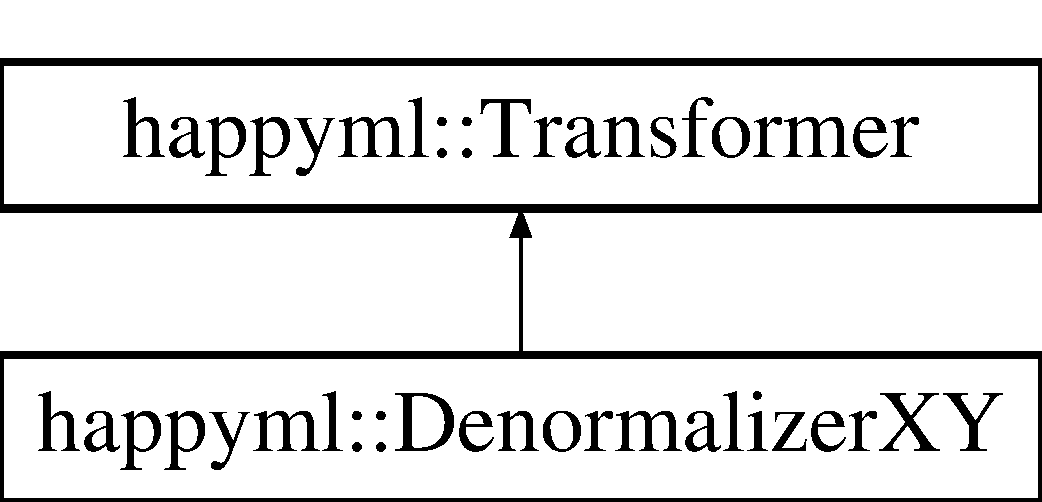
\includegraphics[height=2.000000cm]{classhappyml_1_1DenormalizerXY}
\end{center}
\end{figure}
\subsection*{Public Member Functions}
\begin{DoxyCompactItemize}
\item 
\hyperlink{classhappyml_1_1DenormalizerXY_a1b239c3b51956722ce3905f80e4eef39}{Denormalizer\+XY} (const \hyperlink{classhappyml_1_1NormalizerXY}{Normalizer\+XY} \&n)
\item 
\hyperlink{classhappyml_1_1DenormalizerXY_a4b3fe341234bc43b3d1081551d80b2f1}{Denormalizer\+XY} (const \hyperlink{classhappyml_1_1DataSet}{Data\+Set} \&d)
\item 
\hyperlink{classhappyml_1_1Denormalizer}{Denormalizer} \hyperlink{classhappyml_1_1DenormalizerXY_a0524c3c50116d2d268b8eef1071f6c1b}{get\+DenormalizerX} () const 
\item 
\hyperlink{classhappyml_1_1Denormalizer}{Denormalizer} \hyperlink{classhappyml_1_1DenormalizerXY_ae7bc2c630b4698bf61ea198e7cd98563}{get\+DenormalizerY} () const 
\item 
void \hyperlink{classhappyml_1_1DenormalizerXY_a724e14e520004b2d66611c0e152a9d3b}{apply} (\hyperlink{classhappyml_1_1DataSet}{Data\+Set} \&d) const 
\begin{DoxyCompactList}\small\item\em Applies all the transformations at the given dataset. \end{DoxyCompactList}\item 
\hyperlink{namespacehappyml_a03602d1ec49393790b8a0449f40cd01f}{Input} \hyperlink{classhappyml_1_1DenormalizerXY_a22e45e0e3595ede802dca4c4cf772a73}{apply} (const \hyperlink{namespacehappyml_a03602d1ec49393790b8a0449f40cd01f}{Input} \&input) const 
\begin{DoxyCompactList}\small\item\em Applies all the transformations at the given input. \end{DoxyCompactList}\item 
vec \hyperlink{classhappyml_1_1DenormalizerXY_ab913bbdbdb38eae5f182345d1d9a7014}{apply\+Output} (const vec \&output) const 
\end{DoxyCompactItemize}
\subsection*{Protected Attributes}
\begin{DoxyCompactItemize}
\item 
\hyperlink{classhappyml_1_1Denormalizer}{Denormalizer} \hyperlink{classhappyml_1_1DenormalizerXY_a880bbd3a55a9c6cb4a3a84f145c59774}{dx}
\item 
\hyperlink{classhappyml_1_1Denormalizer}{Denormalizer} \hyperlink{classhappyml_1_1DenormalizerXY_a128d0128d1352665a68a3a2de69fb2a8}{dy}
\end{DoxyCompactItemize}


\subsection{Constructor \& Destructor Documentation}
\index{happyml\+::\+Denormalizer\+XY@{happyml\+::\+Denormalizer\+XY}!Denormalizer\+XY@{Denormalizer\+XY}}
\index{Denormalizer\+XY@{Denormalizer\+XY}!happyml\+::\+Denormalizer\+XY@{happyml\+::\+Denormalizer\+XY}}
\subsubsection[{\texorpdfstring{Denormalizer\+X\+Y(const Normalizer\+X\+Y \&n)}{DenormalizerXY(const NormalizerXY &n)}}]{\setlength{\rightskip}{0pt plus 5cm}happyml\+::\+Denormalizer\+X\+Y\+::\+Denormalizer\+XY (
\begin{DoxyParamCaption}
\item[{const {\bf Normalizer\+XY} \&}]{n}
\end{DoxyParamCaption}
)\hspace{0.3cm}{\ttfamily [inline]}}\hypertarget{classhappyml_1_1DenormalizerXY_a1b239c3b51956722ce3905f80e4eef39}{}\label{classhappyml_1_1DenormalizerXY_a1b239c3b51956722ce3905f80e4eef39}
\index{happyml\+::\+Denormalizer\+XY@{happyml\+::\+Denormalizer\+XY}!Denormalizer\+XY@{Denormalizer\+XY}}
\index{Denormalizer\+XY@{Denormalizer\+XY}!happyml\+::\+Denormalizer\+XY@{happyml\+::\+Denormalizer\+XY}}
\subsubsection[{\texorpdfstring{Denormalizer\+X\+Y(const Data\+Set \&d)}{DenormalizerXY(const DataSet &d)}}]{\setlength{\rightskip}{0pt plus 5cm}happyml\+::\+Denormalizer\+X\+Y\+::\+Denormalizer\+XY (
\begin{DoxyParamCaption}
\item[{const {\bf Data\+Set} \&}]{d}
\end{DoxyParamCaption}
)\hspace{0.3cm}{\ttfamily [inline]}}\hypertarget{classhappyml_1_1DenormalizerXY_a4b3fe341234bc43b3d1081551d80b2f1}{}\label{classhappyml_1_1DenormalizerXY_a4b3fe341234bc43b3d1081551d80b2f1}


\subsection{Member Function Documentation}
\index{happyml\+::\+Denormalizer\+XY@{happyml\+::\+Denormalizer\+XY}!apply@{apply}}
\index{apply@{apply}!happyml\+::\+Denormalizer\+XY@{happyml\+::\+Denormalizer\+XY}}
\subsubsection[{\texorpdfstring{apply(\+Data\+Set \&d) const }{apply(DataSet &d) const }}]{\setlength{\rightskip}{0pt plus 5cm}void happyml\+::\+Denormalizer\+X\+Y\+::apply (
\begin{DoxyParamCaption}
\item[{{\bf Data\+Set} \&}]{dataset}
\end{DoxyParamCaption}
) const\hspace{0.3cm}{\ttfamily [inline]}, {\ttfamily [virtual]}}\hypertarget{classhappyml_1_1DenormalizerXY_a724e14e520004b2d66611c0e152a9d3b}{}\label{classhappyml_1_1DenormalizerXY_a724e14e520004b2d66611c0e152a9d3b}


Applies all the transformations at the given dataset. 


\begin{DoxyParams}{Parameters}
{\em dataset} & Dataset to transform. \\
\hline
\end{DoxyParams}


Reimplemented from \hyperlink{classhappyml_1_1Transformer_a169a2a8434124c1dd8e671bca2cfa71d}{happyml\+::\+Transformer}.

\index{happyml\+::\+Denormalizer\+XY@{happyml\+::\+Denormalizer\+XY}!apply@{apply}}
\index{apply@{apply}!happyml\+::\+Denormalizer\+XY@{happyml\+::\+Denormalizer\+XY}}
\subsubsection[{\texorpdfstring{apply(const Input \&input) const }{apply(const Input &input) const }}]{\setlength{\rightskip}{0pt plus 5cm}{\bf Input} happyml\+::\+Denormalizer\+X\+Y\+::apply (
\begin{DoxyParamCaption}
\item[{const {\bf Input} \&}]{input}
\end{DoxyParamCaption}
) const\hspace{0.3cm}{\ttfamily [inline]}, {\ttfamily [virtual]}}\hypertarget{classhappyml_1_1DenormalizerXY_a22e45e0e3595ede802dca4c4cf772a73}{}\label{classhappyml_1_1DenormalizerXY_a22e45e0e3595ede802dca4c4cf772a73}


Applies all the transformations at the given input. 


\begin{DoxyParams}{Parameters}
{\em input} & Input to transform.\\
\hline
\end{DoxyParams}
\begin{DoxyReturn}{Returns}
A transformated version of the input. 
\end{DoxyReturn}


Reimplemented from \hyperlink{classhappyml_1_1Transformer_a3e0eb67990c90c461466307fdefab45c}{happyml\+::\+Transformer}.

\index{happyml\+::\+Denormalizer\+XY@{happyml\+::\+Denormalizer\+XY}!apply\+Output@{apply\+Output}}
\index{apply\+Output@{apply\+Output}!happyml\+::\+Denormalizer\+XY@{happyml\+::\+Denormalizer\+XY}}
\subsubsection[{\texorpdfstring{apply\+Output(const vec \&output) const }{applyOutput(const vec &output) const }}]{\setlength{\rightskip}{0pt plus 5cm}vec happyml\+::\+Denormalizer\+X\+Y\+::apply\+Output (
\begin{DoxyParamCaption}
\item[{const vec \&}]{output}
\end{DoxyParamCaption}
) const\hspace{0.3cm}{\ttfamily [inline]}}\hypertarget{classhappyml_1_1DenormalizerXY_ab913bbdbdb38eae5f182345d1d9a7014}{}\label{classhappyml_1_1DenormalizerXY_ab913bbdbdb38eae5f182345d1d9a7014}
\index{happyml\+::\+Denormalizer\+XY@{happyml\+::\+Denormalizer\+XY}!get\+DenormalizerX@{get\+DenormalizerX}}
\index{get\+DenormalizerX@{get\+DenormalizerX}!happyml\+::\+Denormalizer\+XY@{happyml\+::\+Denormalizer\+XY}}
\subsubsection[{\texorpdfstring{get\+Denormalizer\+X() const }{getDenormalizerX() const }}]{\setlength{\rightskip}{0pt plus 5cm}{\bf Denormalizer} happyml\+::\+Denormalizer\+X\+Y\+::get\+DenormalizerX (
\begin{DoxyParamCaption}
{}
\end{DoxyParamCaption}
) const\hspace{0.3cm}{\ttfamily [inline]}}\hypertarget{classhappyml_1_1DenormalizerXY_a0524c3c50116d2d268b8eef1071f6c1b}{}\label{classhappyml_1_1DenormalizerXY_a0524c3c50116d2d268b8eef1071f6c1b}
\index{happyml\+::\+Denormalizer\+XY@{happyml\+::\+Denormalizer\+XY}!get\+DenormalizerY@{get\+DenormalizerY}}
\index{get\+DenormalizerY@{get\+DenormalizerY}!happyml\+::\+Denormalizer\+XY@{happyml\+::\+Denormalizer\+XY}}
\subsubsection[{\texorpdfstring{get\+Denormalizer\+Y() const }{getDenormalizerY() const }}]{\setlength{\rightskip}{0pt plus 5cm}{\bf Denormalizer} happyml\+::\+Denormalizer\+X\+Y\+::get\+DenormalizerY (
\begin{DoxyParamCaption}
{}
\end{DoxyParamCaption}
) const\hspace{0.3cm}{\ttfamily [inline]}}\hypertarget{classhappyml_1_1DenormalizerXY_ae7bc2c630b4698bf61ea198e7cd98563}{}\label{classhappyml_1_1DenormalizerXY_ae7bc2c630b4698bf61ea198e7cd98563}


\subsection{Member Data Documentation}
\index{happyml\+::\+Denormalizer\+XY@{happyml\+::\+Denormalizer\+XY}!dx@{dx}}
\index{dx@{dx}!happyml\+::\+Denormalizer\+XY@{happyml\+::\+Denormalizer\+XY}}
\subsubsection[{\texorpdfstring{dx}{dx}}]{\setlength{\rightskip}{0pt plus 5cm}{\bf Denormalizer} happyml\+::\+Denormalizer\+X\+Y\+::dx\hspace{0.3cm}{\ttfamily [protected]}}\hypertarget{classhappyml_1_1DenormalizerXY_a880bbd3a55a9c6cb4a3a84f145c59774}{}\label{classhappyml_1_1DenormalizerXY_a880bbd3a55a9c6cb4a3a84f145c59774}
\index{happyml\+::\+Denormalizer\+XY@{happyml\+::\+Denormalizer\+XY}!dy@{dy}}
\index{dy@{dy}!happyml\+::\+Denormalizer\+XY@{happyml\+::\+Denormalizer\+XY}}
\subsubsection[{\texorpdfstring{dy}{dy}}]{\setlength{\rightskip}{0pt plus 5cm}{\bf Denormalizer} happyml\+::\+Denormalizer\+X\+Y\+::dy\hspace{0.3cm}{\ttfamily [protected]}}\hypertarget{classhappyml_1_1DenormalizerXY_a128d0128d1352665a68a3a2de69fb2a8}{}\label{classhappyml_1_1DenormalizerXY_a128d0128d1352665a68a3a2de69fb2a8}


The documentation for this class was generated from the following file\+:\begin{DoxyCompactItemize}
\item 
include/happyml/transformers/\hyperlink{normalizer_8h}{normalizer.\+h}\end{DoxyCompactItemize}

\hypertarget{classhappyml_1_1Destandarizer}{}\section{happyml\+:\+:Destandarizer Class Reference}
\label{classhappyml_1_1Destandarizer}\index{happyml\+::\+Destandarizer@{happyml\+::\+Destandarizer}}


{\ttfamily \#include $<$standarizer.\+h$>$}

Inheritance diagram for happyml\+:\+:Destandarizer\+:\begin{figure}[H]
\begin{center}
\leavevmode
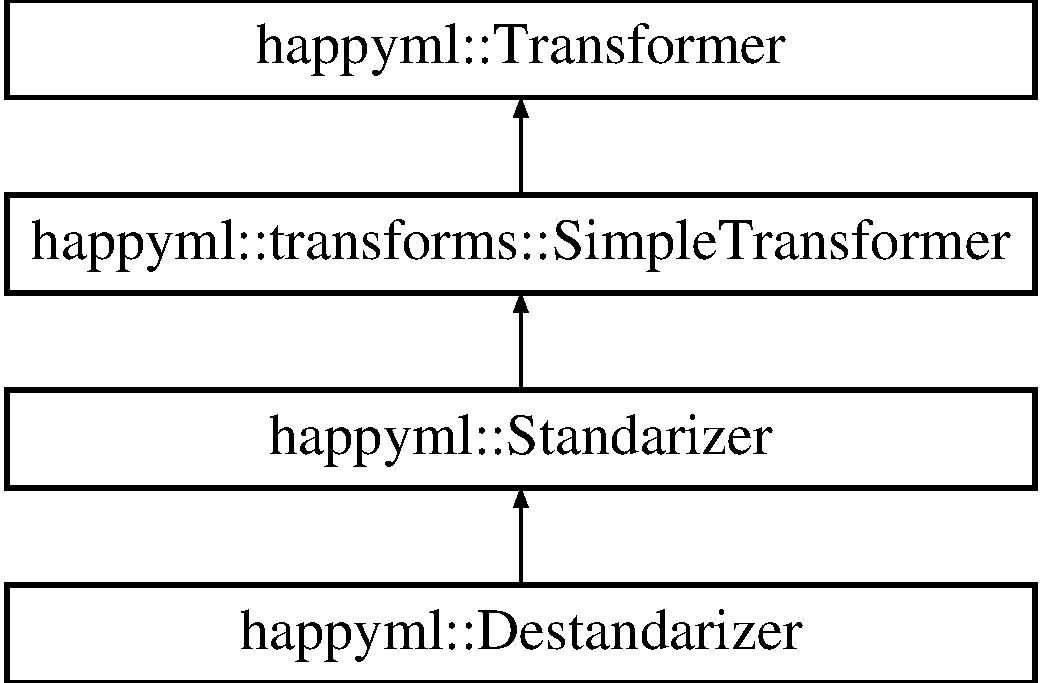
\includegraphics[height=4.000000cm]{classhappyml_1_1Destandarizer}
\end{center}
\end{figure}
\subsection*{Public Member Functions}
\begin{DoxyCompactItemize}
\item 
\hyperlink{classhappyml_1_1Destandarizer_abc64ade944fc341a889ef3b703e294dc}{Destandarizer} (const \hyperlink{classhappyml_1_1DataSet}{Data\+Set} \&dataset)
\begin{DoxyCompactList}\small\item\em Creates a denormalizer that will use min and max data obtained from the dataset. \end{DoxyCompactList}\item 
\hyperlink{classhappyml_1_1Destandarizer_ae8ede809ec02a8a8553fbf0b13d0dc67}{Destandarizer} (const mat \&x)
\begin{DoxyCompactList}\small\item\em Creates a denormalizer that will use min and max data obtained from the matrix x. \end{DoxyCompactList}\item 
\hyperlink{classhappyml_1_1Destandarizer_a248bde27fb7e9befc813a1db7daba7bb}{Destandarizer} (const vec \&minvec, const vec \&maxvec)
\begin{DoxyCompactList}\small\item\em Creates a denormalizer that will use min and max data obtained from the dataset. \end{DoxyCompactList}\item 
\hyperlink{classhappyml_1_1Destandarizer_ad892a74ae3ca529548305cda54969c6e}{Destandarizer} (const \hyperlink{classhappyml_1_1Standarizer}{Standarizer} \&n)
\begin{DoxyCompactList}\small\item\em Creates a denormalizer using the given normalizer. \end{DoxyCompactList}\item 
\hyperlink{classhappyml_1_1Destandarizer_a8e20a4a4d1245217ea0b8eba7b740a6e}{$\sim$\+Destandarizer} ()
\item 
virtual void \hyperlink{classhappyml_1_1Destandarizer_a2d1542f1857bfe0cb23fa69b139d2368}{apply} (mat \&x) const 
\end{DoxyCompactItemize}
\subsection*{Additional Inherited Members}


\subsection{Constructor \& Destructor Documentation}
\index{happyml\+::\+Destandarizer@{happyml\+::\+Destandarizer}!Destandarizer@{Destandarizer}}
\index{Destandarizer@{Destandarizer}!happyml\+::\+Destandarizer@{happyml\+::\+Destandarizer}}
\subsubsection[{\texorpdfstring{Destandarizer(const Data\+Set \&dataset)}{Destandarizer(const DataSet &dataset)}}]{\setlength{\rightskip}{0pt plus 5cm}happyml\+::\+Destandarizer\+::\+Destandarizer (
\begin{DoxyParamCaption}
\item[{const {\bf Data\+Set} \&}]{dataset}
\end{DoxyParamCaption}
)\hspace{0.3cm}{\ttfamily [inline]}}\hypertarget{classhappyml_1_1Destandarizer_abc64ade944fc341a889ef3b703e294dc}{}\label{classhappyml_1_1Destandarizer_abc64ade944fc341a889ef3b703e294dc}


Creates a denormalizer that will use min and max data obtained from the dataset. 


\begin{DoxyParams}{Parameters}
{\em dataset} & Dataset from which it will be extracted the min and max that will be use when apply denormalization. \\
\hline
\end{DoxyParams}
\index{happyml\+::\+Destandarizer@{happyml\+::\+Destandarizer}!Destandarizer@{Destandarizer}}
\index{Destandarizer@{Destandarizer}!happyml\+::\+Destandarizer@{happyml\+::\+Destandarizer}}
\subsubsection[{\texorpdfstring{Destandarizer(const mat \&x)}{Destandarizer(const mat &x)}}]{\setlength{\rightskip}{0pt plus 5cm}happyml\+::\+Destandarizer\+::\+Destandarizer (
\begin{DoxyParamCaption}
\item[{const mat \&}]{x}
\end{DoxyParamCaption}
)\hspace{0.3cm}{\ttfamily [inline]}}\hypertarget{classhappyml_1_1Destandarizer_ae8ede809ec02a8a8553fbf0b13d0dc67}{}\label{classhappyml_1_1Destandarizer_ae8ede809ec02a8a8553fbf0b13d0dc67}


Creates a denormalizer that will use min and max data obtained from the matrix x. 


\begin{DoxyParams}{Parameters}
{\em x} & Matrix from which it will be extracted the min and max that will be use when apply denormalization. \\
\hline
\end{DoxyParams}
\index{happyml\+::\+Destandarizer@{happyml\+::\+Destandarizer}!Destandarizer@{Destandarizer}}
\index{Destandarizer@{Destandarizer}!happyml\+::\+Destandarizer@{happyml\+::\+Destandarizer}}
\subsubsection[{\texorpdfstring{Destandarizer(const vec \&minvec, const vec \&maxvec)}{Destandarizer(const vec &minvec, const vec &maxvec)}}]{\setlength{\rightskip}{0pt plus 5cm}happyml\+::\+Destandarizer\+::\+Destandarizer (
\begin{DoxyParamCaption}
\item[{const vec \&}]{minvec, }
\item[{const vec \&}]{maxvec}
\end{DoxyParamCaption}
)\hspace{0.3cm}{\ttfamily [inline]}}\hypertarget{classhappyml_1_1Destandarizer_a248bde27fb7e9befc813a1db7daba7bb}{}\label{classhappyml_1_1Destandarizer_a248bde27fb7e9befc813a1db7daba7bb}


Creates a denormalizer that will use min and max data obtained from the dataset. 


\begin{DoxyParams}{Parameters}
{\em minvec} & Vector with the min numbers. \\
\hline
{\em maxvec} & Vector with the max numbers. \\
\hline
\end{DoxyParams}
\index{happyml\+::\+Destandarizer@{happyml\+::\+Destandarizer}!Destandarizer@{Destandarizer}}
\index{Destandarizer@{Destandarizer}!happyml\+::\+Destandarizer@{happyml\+::\+Destandarizer}}
\subsubsection[{\texorpdfstring{Destandarizer(const Standarizer \&n)}{Destandarizer(const Standarizer &n)}}]{\setlength{\rightskip}{0pt plus 5cm}happyml\+::\+Destandarizer\+::\+Destandarizer (
\begin{DoxyParamCaption}
\item[{const {\bf Standarizer} \&}]{n}
\end{DoxyParamCaption}
)\hspace{0.3cm}{\ttfamily [inline]}}\hypertarget{classhappyml_1_1Destandarizer_ad892a74ae3ca529548305cda54969c6e}{}\label{classhappyml_1_1Destandarizer_ad892a74ae3ca529548305cda54969c6e}


Creates a denormalizer using the given normalizer. 


\begin{DoxyParams}{Parameters}
{\em n} & \hyperlink{classhappyml_1_1Normalizer}{Normalizer} to reverse. \\
\hline
\end{DoxyParams}
\index{happyml\+::\+Destandarizer@{happyml\+::\+Destandarizer}!````~Destandarizer@{$\sim$\+Destandarizer}}
\index{````~Destandarizer@{$\sim$\+Destandarizer}!happyml\+::\+Destandarizer@{happyml\+::\+Destandarizer}}
\subsubsection[{\texorpdfstring{$\sim$\+Destandarizer()}{~Destandarizer()}}]{\setlength{\rightskip}{0pt plus 5cm}happyml\+::\+Destandarizer\+::$\sim$\+Destandarizer (
\begin{DoxyParamCaption}
{}
\end{DoxyParamCaption}
)\hspace{0.3cm}{\ttfamily [inline]}}\hypertarget{classhappyml_1_1Destandarizer_a8e20a4a4d1245217ea0b8eba7b740a6e}{}\label{classhappyml_1_1Destandarizer_a8e20a4a4d1245217ea0b8eba7b740a6e}


\subsection{Member Function Documentation}
\index{happyml\+::\+Destandarizer@{happyml\+::\+Destandarizer}!apply@{apply}}
\index{apply@{apply}!happyml\+::\+Destandarizer@{happyml\+::\+Destandarizer}}
\subsubsection[{\texorpdfstring{apply(mat \&x) const }{apply(mat &x) const }}]{\setlength{\rightskip}{0pt plus 5cm}void happyml\+::\+Destandarizer\+::apply (
\begin{DoxyParamCaption}
\item[{mat \&}]{x}
\end{DoxyParamCaption}
) const\hspace{0.3cm}{\ttfamily [virtual]}}\hypertarget{classhappyml_1_1Destandarizer_a2d1542f1857bfe0cb23fa69b139d2368}{}\label{classhappyml_1_1Destandarizer_a2d1542f1857bfe0cb23fa69b139d2368}


Reimplemented from \hyperlink{classhappyml_1_1Standarizer_a5c9b416b657cb61972c27b27fd379b2d}{happyml\+::\+Standarizer}.



The documentation for this class was generated from the following files\+:\begin{DoxyCompactItemize}
\item 
include/happyml/transformers/\hyperlink{standarizer_8h}{standarizer.\+h}\item 
src/transformers/\hyperlink{standarizer_8cpp}{standarizer.\+cpp}\end{DoxyCompactItemize}

\hypertarget{classhappyml_1_1DestandarizerXY}{}\section{happyml\+:\+:Destandarizer\+XY Class Reference}
\label{classhappyml_1_1DestandarizerXY}\index{happyml\+::\+Destandarizer\+XY@{happyml\+::\+Destandarizer\+XY}}


{\ttfamily \#include $<$standarizer.\+h$>$}

Inheritance diagram for happyml\+:\+:Destandarizer\+XY\+:\begin{figure}[H]
\begin{center}
\leavevmode
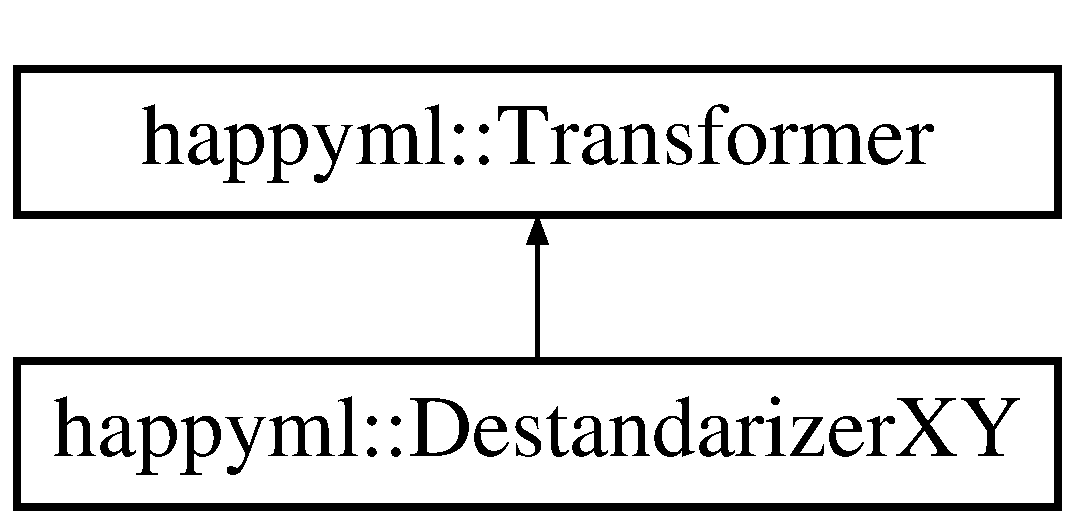
\includegraphics[height=2.000000cm]{classhappyml_1_1DestandarizerXY}
\end{center}
\end{figure}
\subsection*{Public Member Functions}
\begin{DoxyCompactItemize}
\item 
\hyperlink{classhappyml_1_1DestandarizerXY_a3acaf6aea99a5c5fdc3e6f4cd22d82bd}{Destandarizer\+XY} (const \hyperlink{classhappyml_1_1StandarizerXY}{Standarizer\+XY} \&n)
\item 
\hyperlink{classhappyml_1_1DestandarizerXY_aa2ad85844e63d1f359ac867e6eaa321e}{Destandarizer\+XY} (const \hyperlink{classhappyml_1_1DataSet}{Data\+Set} \&d)
\item 
\hyperlink{classhappyml_1_1Destandarizer}{Destandarizer} \hyperlink{classhappyml_1_1DestandarizerXY_a3c6a17ec4130156001573205e0a313f6}{get\+DestandarizerX} () const 
\item 
\hyperlink{classhappyml_1_1Destandarizer}{Destandarizer} \hyperlink{classhappyml_1_1DestandarizerXY_ad4b4914107d212cc5167269beb99c21e}{get\+DestandarizerY} () const 
\item 
void \hyperlink{classhappyml_1_1DestandarizerXY_a84c63216d9a78bc61647550381fed0a6}{apply} (\hyperlink{classhappyml_1_1DataSet}{Data\+Set} \&d) const 
\begin{DoxyCompactList}\small\item\em Applies all the transformations at the given dataset. \end{DoxyCompactList}\item 
\hyperlink{namespacehappyml_a03602d1ec49393790b8a0449f40cd01f}{Input} \hyperlink{classhappyml_1_1DestandarizerXY_a21481d414441642b50b04d43f6c55ac0}{apply} (const \hyperlink{namespacehappyml_a03602d1ec49393790b8a0449f40cd01f}{Input} \&input) const 
\begin{DoxyCompactList}\small\item\em Applies all the transformations at the given input. \end{DoxyCompactList}\item 
vec \hyperlink{classhappyml_1_1DestandarizerXY_a09d965fba7e7dfb174cbd7fbd84ac24b}{apply\+Output} (const vec \&output) const 
\end{DoxyCompactItemize}
\subsection*{Protected Attributes}
\begin{DoxyCompactItemize}
\item 
\hyperlink{classhappyml_1_1Destandarizer}{Destandarizer} \hyperlink{classhappyml_1_1DestandarizerXY_aeaa319686a49d6a844cd4c2a259c97ef}{dx}
\item 
\hyperlink{classhappyml_1_1Destandarizer}{Destandarizer} \hyperlink{classhappyml_1_1DestandarizerXY_ac482475137a51829da3d1a9f99817960}{dy}
\end{DoxyCompactItemize}


\subsection{Constructor \& Destructor Documentation}
\index{happyml\+::\+Destandarizer\+XY@{happyml\+::\+Destandarizer\+XY}!Destandarizer\+XY@{Destandarizer\+XY}}
\index{Destandarizer\+XY@{Destandarizer\+XY}!happyml\+::\+Destandarizer\+XY@{happyml\+::\+Destandarizer\+XY}}
\subsubsection[{\texorpdfstring{Destandarizer\+X\+Y(const Standarizer\+X\+Y \&n)}{DestandarizerXY(const StandarizerXY &n)}}]{\setlength{\rightskip}{0pt plus 5cm}happyml\+::\+Destandarizer\+X\+Y\+::\+Destandarizer\+XY (
\begin{DoxyParamCaption}
\item[{const {\bf Standarizer\+XY} \&}]{n}
\end{DoxyParamCaption}
)\hspace{0.3cm}{\ttfamily [inline]}}\hypertarget{classhappyml_1_1DestandarizerXY_a3acaf6aea99a5c5fdc3e6f4cd22d82bd}{}\label{classhappyml_1_1DestandarizerXY_a3acaf6aea99a5c5fdc3e6f4cd22d82bd}
\index{happyml\+::\+Destandarizer\+XY@{happyml\+::\+Destandarizer\+XY}!Destandarizer\+XY@{Destandarizer\+XY}}
\index{Destandarizer\+XY@{Destandarizer\+XY}!happyml\+::\+Destandarizer\+XY@{happyml\+::\+Destandarizer\+XY}}
\subsubsection[{\texorpdfstring{Destandarizer\+X\+Y(const Data\+Set \&d)}{DestandarizerXY(const DataSet &d)}}]{\setlength{\rightskip}{0pt plus 5cm}happyml\+::\+Destandarizer\+X\+Y\+::\+Destandarizer\+XY (
\begin{DoxyParamCaption}
\item[{const {\bf Data\+Set} \&}]{d}
\end{DoxyParamCaption}
)\hspace{0.3cm}{\ttfamily [inline]}}\hypertarget{classhappyml_1_1DestandarizerXY_aa2ad85844e63d1f359ac867e6eaa321e}{}\label{classhappyml_1_1DestandarizerXY_aa2ad85844e63d1f359ac867e6eaa321e}


\subsection{Member Function Documentation}
\index{happyml\+::\+Destandarizer\+XY@{happyml\+::\+Destandarizer\+XY}!apply@{apply}}
\index{apply@{apply}!happyml\+::\+Destandarizer\+XY@{happyml\+::\+Destandarizer\+XY}}
\subsubsection[{\texorpdfstring{apply(\+Data\+Set \&d) const }{apply(DataSet &d) const }}]{\setlength{\rightskip}{0pt plus 5cm}void happyml\+::\+Destandarizer\+X\+Y\+::apply (
\begin{DoxyParamCaption}
\item[{{\bf Data\+Set} \&}]{dataset}
\end{DoxyParamCaption}
) const\hspace{0.3cm}{\ttfamily [inline]}, {\ttfamily [virtual]}}\hypertarget{classhappyml_1_1DestandarizerXY_a84c63216d9a78bc61647550381fed0a6}{}\label{classhappyml_1_1DestandarizerXY_a84c63216d9a78bc61647550381fed0a6}


Applies all the transformations at the given dataset. 


\begin{DoxyParams}{Parameters}
{\em dataset} & Dataset to transform. \\
\hline
\end{DoxyParams}


Reimplemented from \hyperlink{classhappyml_1_1Transformer_a169a2a8434124c1dd8e671bca2cfa71d}{happyml\+::\+Transformer}.

\index{happyml\+::\+Destandarizer\+XY@{happyml\+::\+Destandarizer\+XY}!apply@{apply}}
\index{apply@{apply}!happyml\+::\+Destandarizer\+XY@{happyml\+::\+Destandarizer\+XY}}
\subsubsection[{\texorpdfstring{apply(const Input \&input) const }{apply(const Input &input) const }}]{\setlength{\rightskip}{0pt plus 5cm}{\bf Input} happyml\+::\+Destandarizer\+X\+Y\+::apply (
\begin{DoxyParamCaption}
\item[{const {\bf Input} \&}]{input}
\end{DoxyParamCaption}
) const\hspace{0.3cm}{\ttfamily [inline]}, {\ttfamily [virtual]}}\hypertarget{classhappyml_1_1DestandarizerXY_a21481d414441642b50b04d43f6c55ac0}{}\label{classhappyml_1_1DestandarizerXY_a21481d414441642b50b04d43f6c55ac0}


Applies all the transformations at the given input. 


\begin{DoxyParams}{Parameters}
{\em input} & Input to transform.\\
\hline
\end{DoxyParams}
\begin{DoxyReturn}{Returns}
A transformated version of the input. 
\end{DoxyReturn}


Reimplemented from \hyperlink{classhappyml_1_1Transformer_a3e0eb67990c90c461466307fdefab45c}{happyml\+::\+Transformer}.

\index{happyml\+::\+Destandarizer\+XY@{happyml\+::\+Destandarizer\+XY}!apply\+Output@{apply\+Output}}
\index{apply\+Output@{apply\+Output}!happyml\+::\+Destandarizer\+XY@{happyml\+::\+Destandarizer\+XY}}
\subsubsection[{\texorpdfstring{apply\+Output(const vec \&output) const }{applyOutput(const vec &output) const }}]{\setlength{\rightskip}{0pt plus 5cm}vec happyml\+::\+Destandarizer\+X\+Y\+::apply\+Output (
\begin{DoxyParamCaption}
\item[{const vec \&}]{output}
\end{DoxyParamCaption}
) const\hspace{0.3cm}{\ttfamily [inline]}}\hypertarget{classhappyml_1_1DestandarizerXY_a09d965fba7e7dfb174cbd7fbd84ac24b}{}\label{classhappyml_1_1DestandarizerXY_a09d965fba7e7dfb174cbd7fbd84ac24b}
\index{happyml\+::\+Destandarizer\+XY@{happyml\+::\+Destandarizer\+XY}!get\+DestandarizerX@{get\+DestandarizerX}}
\index{get\+DestandarizerX@{get\+DestandarizerX}!happyml\+::\+Destandarizer\+XY@{happyml\+::\+Destandarizer\+XY}}
\subsubsection[{\texorpdfstring{get\+Destandarizer\+X() const }{getDestandarizerX() const }}]{\setlength{\rightskip}{0pt plus 5cm}{\bf Destandarizer} happyml\+::\+Destandarizer\+X\+Y\+::get\+DestandarizerX (
\begin{DoxyParamCaption}
{}
\end{DoxyParamCaption}
) const\hspace{0.3cm}{\ttfamily [inline]}}\hypertarget{classhappyml_1_1DestandarizerXY_a3c6a17ec4130156001573205e0a313f6}{}\label{classhappyml_1_1DestandarizerXY_a3c6a17ec4130156001573205e0a313f6}
\index{happyml\+::\+Destandarizer\+XY@{happyml\+::\+Destandarizer\+XY}!get\+DestandarizerY@{get\+DestandarizerY}}
\index{get\+DestandarizerY@{get\+DestandarizerY}!happyml\+::\+Destandarizer\+XY@{happyml\+::\+Destandarizer\+XY}}
\subsubsection[{\texorpdfstring{get\+Destandarizer\+Y() const }{getDestandarizerY() const }}]{\setlength{\rightskip}{0pt plus 5cm}{\bf Destandarizer} happyml\+::\+Destandarizer\+X\+Y\+::get\+DestandarizerY (
\begin{DoxyParamCaption}
{}
\end{DoxyParamCaption}
) const\hspace{0.3cm}{\ttfamily [inline]}}\hypertarget{classhappyml_1_1DestandarizerXY_ad4b4914107d212cc5167269beb99c21e}{}\label{classhappyml_1_1DestandarizerXY_ad4b4914107d212cc5167269beb99c21e}


\subsection{Member Data Documentation}
\index{happyml\+::\+Destandarizer\+XY@{happyml\+::\+Destandarizer\+XY}!dx@{dx}}
\index{dx@{dx}!happyml\+::\+Destandarizer\+XY@{happyml\+::\+Destandarizer\+XY}}
\subsubsection[{\texorpdfstring{dx}{dx}}]{\setlength{\rightskip}{0pt plus 5cm}{\bf Destandarizer} happyml\+::\+Destandarizer\+X\+Y\+::dx\hspace{0.3cm}{\ttfamily [protected]}}\hypertarget{classhappyml_1_1DestandarizerXY_aeaa319686a49d6a844cd4c2a259c97ef}{}\label{classhappyml_1_1DestandarizerXY_aeaa319686a49d6a844cd4c2a259c97ef}
\index{happyml\+::\+Destandarizer\+XY@{happyml\+::\+Destandarizer\+XY}!dy@{dy}}
\index{dy@{dy}!happyml\+::\+Destandarizer\+XY@{happyml\+::\+Destandarizer\+XY}}
\subsubsection[{\texorpdfstring{dy}{dy}}]{\setlength{\rightskip}{0pt plus 5cm}{\bf Destandarizer} happyml\+::\+Destandarizer\+X\+Y\+::dy\hspace{0.3cm}{\ttfamily [protected]}}\hypertarget{classhappyml_1_1DestandarizerXY_ac482475137a51829da3d1a9f99817960}{}\label{classhappyml_1_1DestandarizerXY_ac482475137a51829da3d1a9f99817960}


The documentation for this class was generated from the following file\+:\begin{DoxyCompactItemize}
\item 
include/happyml/transformers/\hyperlink{standarizer_8h}{standarizer.\+h}\end{DoxyCompactItemize}

\hypertarget{classhappyml_1_1KFoldCrossValidation}{}\section{happyml\+:\+:K\+Fold\+Cross\+Validation Class Reference}
\label{classhappyml_1_1KFoldCrossValidation}\index{happyml\+::\+K\+Fold\+Cross\+Validation@{happyml\+::\+K\+Fold\+Cross\+Validation}}


{\ttfamily \#include $<$k\+\_\+fold\+\_\+cross\+\_\+validation.\+h$>$}

\subsection*{Static Public Member Functions}
\begin{DoxyCompactItemize}
\item 
static void \hyperlink{classhappyml_1_1KFoldCrossValidation_a54618117f5acf9b97fd521b98e29227d}{apply} (const \hyperlink{classhappyml_1_1DataSet}{Data\+Set} \&dataset, int n, \hyperlink{classhappyml_1_1TrainingProcess}{Training\+Process} \&process)
\end{DoxyCompactItemize}


\subsection{Member Function Documentation}
\index{happyml\+::\+K\+Fold\+Cross\+Validation@{happyml\+::\+K\+Fold\+Cross\+Validation}!apply@{apply}}
\index{apply@{apply}!happyml\+::\+K\+Fold\+Cross\+Validation@{happyml\+::\+K\+Fold\+Cross\+Validation}}
\subsubsection[{\texorpdfstring{apply(const Data\+Set \&dataset, int n, Training\+Process \&process)}{apply(const DataSet &dataset, int n, TrainingProcess &process)}}]{\setlength{\rightskip}{0pt plus 5cm}void happyml\+::\+K\+Fold\+Cross\+Validation\+::apply (
\begin{DoxyParamCaption}
\item[{const {\bf Data\+Set} \&}]{dataset, }
\item[{int}]{n, }
\item[{{\bf Training\+Process} \&}]{process}
\end{DoxyParamCaption}
)\hspace{0.3cm}{\ttfamily [static]}}\hypertarget{classhappyml_1_1KFoldCrossValidation_a54618117f5acf9b97fd521b98e29227d}{}\label{classhappyml_1_1KFoldCrossValidation_a54618117f5acf9b97fd521b98e29227d}

\begin{DoxyParams}{Parameters}
{\em dataset} & Dataset to devide. \\
\hline
{\em n} & Number of divisions. \\
\hline
{\em process} & Training process to repeat for each fold. \\
\hline
\end{DoxyParams}


The documentation for this class was generated from the following files\+:\begin{DoxyCompactItemize}
\item 
include/happyml/\hyperlink{k__fold__cross__validation_8h}{k\+\_\+fold\+\_\+cross\+\_\+validation.\+h}\item 
src/\hyperlink{k__fold__cross__validation_8cpp}{k\+\_\+fold\+\_\+cross\+\_\+validation.\+cpp}\end{DoxyCompactItemize}

\hypertarget{classhappyml_1_1KNN}{}\section{happyml\+:\+:K\+NN Class Reference}
\label{classhappyml_1_1KNN}\index{happyml\+::\+K\+NN@{happyml\+::\+K\+NN}}


{\ttfamily \#include $<$knn.\+h$>$}

Inheritance diagram for happyml\+:\+:K\+NN\+:\begin{figure}[H]
\begin{center}
\leavevmode
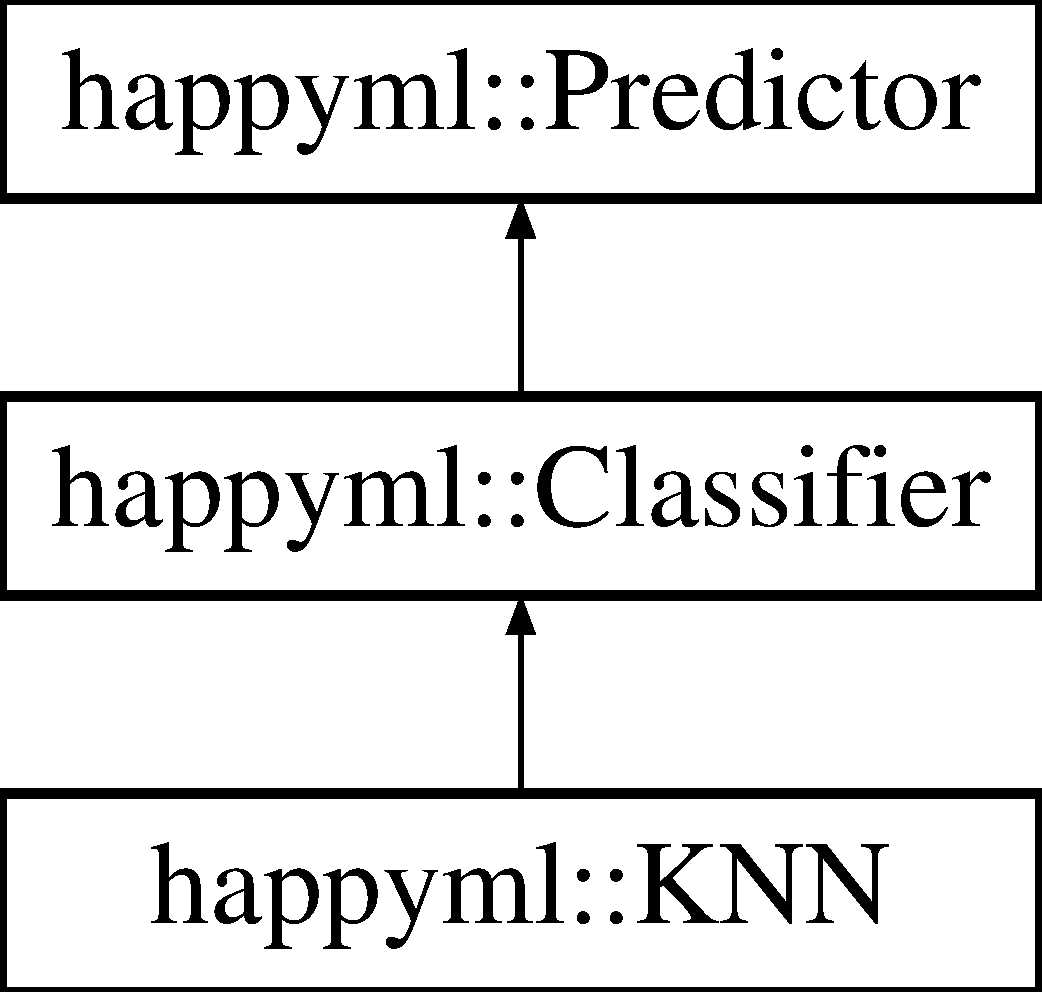
\includegraphics[height=3.000000cm]{classhappyml_1_1KNN}
\end{center}
\end{figure}
\subsection*{Public Member Functions}
\begin{DoxyCompactItemize}
\item 
\hyperlink{classhappyml_1_1KNN_a369c46398ffc867423133aaf1c7a5a02}{K\+NN} (const \hyperlink{classhappyml_1_1DataSet}{Data\+Set} \&d, int k=1)
\begin{DoxyCompactList}\small\item\em Creates a \hyperlink{classhappyml_1_1KNN}{K\+NN} classifier that uses the indicated training set. \end{DoxyCompactList}\item 
\hyperlink{classhappyml_1_1KNN_a0c93adb094f8c380b8f38aace10ea6e6}{K\+NN} (const \hyperlink{classhappyml_1_1KNN}{K\+NN} \&knn)
\item 
double \hyperlink{classhappyml_1_1KNN_aac58df51b7b343dfd1fb359117341867}{predict} (const \hyperlink{namespacehappyml_a03602d1ec49393790b8a0449f40cd01f}{Input} \&x) const 
\begin{DoxyCompactList}\small\item\em Classifies an input vector. \end{DoxyCompactList}\item 
void \hyperlink{classhappyml_1_1KNN_adb49a173a9ed23725c23964cd333b686}{setK} (int k)
\item 
int \hyperlink{classhappyml_1_1KNN_a66ebb208b2c3138c6d7b23d8204103b7}{getK} ()
\end{DoxyCompactItemize}


\subsection{Constructor \& Destructor Documentation}
\index{happyml\+::\+K\+NN@{happyml\+::\+K\+NN}!K\+NN@{K\+NN}}
\index{K\+NN@{K\+NN}!happyml\+::\+K\+NN@{happyml\+::\+K\+NN}}
\subsubsection[{\texorpdfstring{K\+N\+N(const Data\+Set \&d, int k=1)}{KNN(const DataSet &d, int k=1)}}]{\setlength{\rightskip}{0pt plus 5cm}happyml\+::\+K\+N\+N\+::\+K\+NN (
\begin{DoxyParamCaption}
\item[{const {\bf Data\+Set} \&}]{d, }
\item[{int}]{k = {\ttfamily 1}}
\end{DoxyParamCaption}
)\hspace{0.3cm}{\ttfamily [inline]}}\hypertarget{classhappyml_1_1KNN_a369c46398ffc867423133aaf1c7a5a02}{}\label{classhappyml_1_1KNN_a369c46398ffc867423133aaf1c7a5a02}


Creates a \hyperlink{classhappyml_1_1KNN}{K\+NN} classifier that uses the indicated training set. 


\begin{DoxyParams}{Parameters}
{\em d} & Training set used to compute distances. \\
\hline
\end{DoxyParams}
\index{happyml\+::\+K\+NN@{happyml\+::\+K\+NN}!K\+NN@{K\+NN}}
\index{K\+NN@{K\+NN}!happyml\+::\+K\+NN@{happyml\+::\+K\+NN}}
\subsubsection[{\texorpdfstring{K\+N\+N(const K\+N\+N \&knn)}{KNN(const KNN &knn)}}]{\setlength{\rightskip}{0pt plus 5cm}happyml\+::\+K\+N\+N\+::\+K\+NN (
\begin{DoxyParamCaption}
\item[{const {\bf K\+NN} \&}]{knn}
\end{DoxyParamCaption}
)\hspace{0.3cm}{\ttfamily [inline]}}\hypertarget{classhappyml_1_1KNN_a0c93adb094f8c380b8f38aace10ea6e6}{}\label{classhappyml_1_1KNN_a0c93adb094f8c380b8f38aace10ea6e6}


\subsection{Member Function Documentation}
\index{happyml\+::\+K\+NN@{happyml\+::\+K\+NN}!getK@{getK}}
\index{getK@{getK}!happyml\+::\+K\+NN@{happyml\+::\+K\+NN}}
\subsubsection[{\texorpdfstring{get\+K()}{getK()}}]{\setlength{\rightskip}{0pt plus 5cm}int happyml\+::\+K\+N\+N\+::getK (
\begin{DoxyParamCaption}
{}
\end{DoxyParamCaption}
)\hspace{0.3cm}{\ttfamily [inline]}}\hypertarget{classhappyml_1_1KNN_a66ebb208b2c3138c6d7b23d8204103b7}{}\label{classhappyml_1_1KNN_a66ebb208b2c3138c6d7b23d8204103b7}
\index{happyml\+::\+K\+NN@{happyml\+::\+K\+NN}!predict@{predict}}
\index{predict@{predict}!happyml\+::\+K\+NN@{happyml\+::\+K\+NN}}
\subsubsection[{\texorpdfstring{predict(const Input \&x) const }{predict(const Input &x) const }}]{\setlength{\rightskip}{0pt plus 5cm}double happyml\+::\+K\+N\+N\+::predict (
\begin{DoxyParamCaption}
\item[{const {\bf Input} \&}]{x}
\end{DoxyParamCaption}
) const\hspace{0.3cm}{\ttfamily [virtual]}}\hypertarget{classhappyml_1_1KNN_aac58df51b7b343dfd1fb359117341867}{}\label{classhappyml_1_1KNN_aac58df51b7b343dfd1fb359117341867}


Classifies an input vector. 

\begin{DoxyReturn}{Returns}
Number of the output of the nearest point in the training set. 
\end{DoxyReturn}


Implements \hyperlink{classhappyml_1_1Predictor_a07cf89d655e7642fd94c9b2a8fd0a04b}{happyml\+::\+Predictor}.

\index{happyml\+::\+K\+NN@{happyml\+::\+K\+NN}!setK@{setK}}
\index{setK@{setK}!happyml\+::\+K\+NN@{happyml\+::\+K\+NN}}
\subsubsection[{\texorpdfstring{set\+K(int k)}{setK(int k)}}]{\setlength{\rightskip}{0pt plus 5cm}void happyml\+::\+K\+N\+N\+::setK (
\begin{DoxyParamCaption}
\item[{int}]{k}
\end{DoxyParamCaption}
)\hspace{0.3cm}{\ttfamily [inline]}}\hypertarget{classhappyml_1_1KNN_adb49a173a9ed23725c23964cd333b686}{}\label{classhappyml_1_1KNN_adb49a173a9ed23725c23964cd333b686}


The documentation for this class was generated from the following files\+:\begin{DoxyCompactItemize}
\item 
include/happyml/knn/\hyperlink{knn_8h}{knn.\+h}\item 
src/knn/\hyperlink{knn_8cpp}{knn.\+cpp}\end{DoxyCompactItemize}

\hypertarget{classhappyml_1_1LDA}{}\section{happyml\+:\+:L\+DA Class Reference}
\label{classhappyml_1_1LDA}\index{happyml\+::\+L\+DA@{happyml\+::\+L\+DA}}


Dimensionality reduction using \hyperlink{classhappyml_1_1LDA}{L\+DA}.  




{\ttfamily \#include $<$lda.\+h$>$}

Inheritance diagram for happyml\+:\+:L\+DA\+:\begin{figure}[H]
\begin{center}
\leavevmode
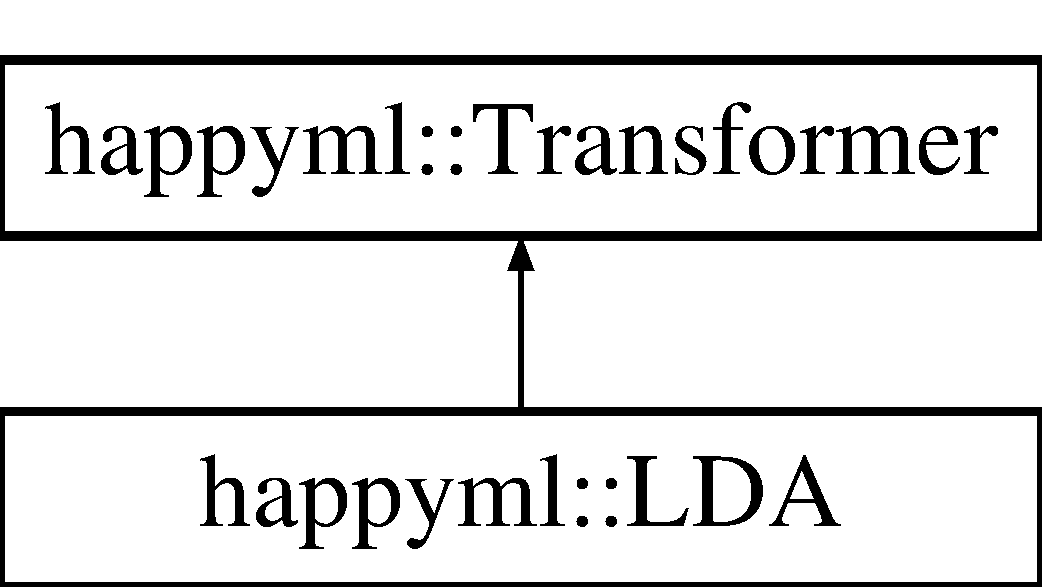
\includegraphics[height=2.000000cm]{classhappyml_1_1LDA}
\end{center}
\end{figure}
\subsection*{Public Member Functions}
\begin{DoxyCompactItemize}
\item 
\hyperlink{classhappyml_1_1LDA_a999cf366ac462e1c22452b0a2b0c9298}{L\+DA} (const \hyperlink{classhappyml_1_1DataSet}{Data\+Set} \&dataset, double n)
\begin{DoxyCompactList}\small\item\em Creates a \hyperlink{classhappyml_1_1LDA}{L\+DA} extractor using the dataset data. \end{DoxyCompactList}\item 
\hyperlink{classhappyml_1_1LDA_a48b3e54c10cece4086005ee65ed405e8}{$\sim$\+L\+DA} ()
\item 
double \hyperlink{classhappyml_1_1LDA_a51210380f50380f77644fabbe1a89614}{get\+Retained\+Variance} () const 
\begin{DoxyCompactList}\small\item\em Returns the retained data variance of the \hyperlink{classhappyml_1_1LDA}{L\+DA} transformation. \end{DoxyCompactList}\item 
void \hyperlink{classhappyml_1_1LDA_a642ebe3b7cfcddaa5b21cd93ed1cf082}{apply} (\hyperlink{classhappyml_1_1DataSet}{Data\+Set} \&dataset) const 
\begin{DoxyCompactList}\small\item\em Applies all the transformations at the given dataset. \end{DoxyCompactList}\item 
void \hyperlink{classhappyml_1_1LDA_aca3f8a0da485bc1d6804fb0dc76dd4fc}{apply} (mat \&x) const 
\item 
\hyperlink{namespacehappyml_a03602d1ec49393790b8a0449f40cd01f}{Input} \hyperlink{classhappyml_1_1LDA_a2b98a4675abdb0985347491224136b5c}{apply} (const \hyperlink{namespacehappyml_a03602d1ec49393790b8a0449f40cd01f}{Input} \&input) const 
\begin{DoxyCompactList}\small\item\em Applies all the transformations at the given input. \end{DoxyCompactList}\end{DoxyCompactItemize}
\subsection*{Protected Attributes}
\begin{DoxyCompactItemize}
\item 
rowvec \hyperlink{classhappyml_1_1LDA_a48e66fff3b5c1609ae8c8de7fae607dd}{mean\+Vec}
\item 
vec \hyperlink{classhappyml_1_1LDA_a72cc9a99337b9262197b0954a78807aa}{eig\+Val}
\item 
mat \hyperlink{classhappyml_1_1LDA_aaf2e27b8502467166802e288e3d1a404}{eig\+Vec}
\item 
mat \hyperlink{classhappyml_1_1LDA_a41be2a7abe7e7c7b4dd389ae163d8028}{cov\+Mat}
\item 
int \hyperlink{classhappyml_1_1LDA_ae9ac22c7ace3bcc924d9d104fafe7e6d}{k}
\item 
double \hyperlink{classhappyml_1_1LDA_a0af7e26335458930d1a5a2006057c9fe}{min\+Var}
\end{DoxyCompactItemize}


\subsection{Detailed Description}
Dimensionality reduction using \hyperlink{classhappyml_1_1LDA}{L\+DA}. 

\subsection{Constructor \& Destructor Documentation}
\index{happyml\+::\+L\+DA@{happyml\+::\+L\+DA}!L\+DA@{L\+DA}}
\index{L\+DA@{L\+DA}!happyml\+::\+L\+DA@{happyml\+::\+L\+DA}}
\subsubsection[{\texorpdfstring{L\+D\+A(const Data\+Set \&dataset, double n)}{LDA(const DataSet &dataset, double n)}}]{\setlength{\rightskip}{0pt plus 5cm}happyml\+::\+L\+D\+A\+::\+L\+DA (
\begin{DoxyParamCaption}
\item[{const {\bf Data\+Set} \&}]{dataset, }
\item[{double}]{n}
\end{DoxyParamCaption}
)}\hypertarget{classhappyml_1_1LDA_a999cf366ac462e1c22452b0a2b0c9298}{}\label{classhappyml_1_1LDA_a999cf366ac462e1c22452b0a2b0c9298}


Creates a \hyperlink{classhappyml_1_1LDA}{L\+DA} extractor using the dataset data. 


\begin{DoxyParams}{Parameters}
{\em dataset} & Dataset from which the eigenvecs for the \hyperlink{classhappyml_1_1LDA}{L\+DA} will be extracted. \\
\hline
{\em n} & Number of dimension to preserve or min mariance if it is a number between 0 and 1. \\
\hline
\end{DoxyParams}
\index{happyml\+::\+L\+DA@{happyml\+::\+L\+DA}!````~L\+DA@{$\sim$\+L\+DA}}
\index{````~L\+DA@{$\sim$\+L\+DA}!happyml\+::\+L\+DA@{happyml\+::\+L\+DA}}
\subsubsection[{\texorpdfstring{$\sim$\+L\+D\+A()}{~LDA()}}]{\setlength{\rightskip}{0pt plus 5cm}happyml\+::\+L\+D\+A\+::$\sim$\+L\+DA (
\begin{DoxyParamCaption}
{}
\end{DoxyParamCaption}
)\hspace{0.3cm}{\ttfamily [inline]}}\hypertarget{classhappyml_1_1LDA_a48b3e54c10cece4086005ee65ed405e8}{}\label{classhappyml_1_1LDA_a48b3e54c10cece4086005ee65ed405e8}


\subsection{Member Function Documentation}
\index{happyml\+::\+L\+DA@{happyml\+::\+L\+DA}!apply@{apply}}
\index{apply@{apply}!happyml\+::\+L\+DA@{happyml\+::\+L\+DA}}
\subsubsection[{\texorpdfstring{apply(\+Data\+Set \&dataset) const }{apply(DataSet &dataset) const }}]{\setlength{\rightskip}{0pt plus 5cm}void happyml\+::\+L\+D\+A\+::apply (
\begin{DoxyParamCaption}
\item[{{\bf Data\+Set} \&}]{dataset}
\end{DoxyParamCaption}
) const\hspace{0.3cm}{\ttfamily [virtual]}}\hypertarget{classhappyml_1_1LDA_a642ebe3b7cfcddaa5b21cd93ed1cf082}{}\label{classhappyml_1_1LDA_a642ebe3b7cfcddaa5b21cd93ed1cf082}


Applies all the transformations at the given dataset. 


\begin{DoxyParams}{Parameters}
{\em dataset} & Dataset to transform. \\
\hline
\end{DoxyParams}


Reimplemented from \hyperlink{classhappyml_1_1Transformer_a169a2a8434124c1dd8e671bca2cfa71d}{happyml\+::\+Transformer}.

\index{happyml\+::\+L\+DA@{happyml\+::\+L\+DA}!apply@{apply}}
\index{apply@{apply}!happyml\+::\+L\+DA@{happyml\+::\+L\+DA}}
\subsubsection[{\texorpdfstring{apply(mat \&x) const }{apply(mat &x) const }}]{\setlength{\rightskip}{0pt plus 5cm}void happyml\+::\+L\+D\+A\+::apply (
\begin{DoxyParamCaption}
\item[{mat \&}]{x}
\end{DoxyParamCaption}
) const}\hypertarget{classhappyml_1_1LDA_aca3f8a0da485bc1d6804fb0dc76dd4fc}{}\label{classhappyml_1_1LDA_aca3f8a0da485bc1d6804fb0dc76dd4fc}
\index{happyml\+::\+L\+DA@{happyml\+::\+L\+DA}!apply@{apply}}
\index{apply@{apply}!happyml\+::\+L\+DA@{happyml\+::\+L\+DA}}
\subsubsection[{\texorpdfstring{apply(const Input \&input) const }{apply(const Input &input) const }}]{\setlength{\rightskip}{0pt plus 5cm}{\bf Input} happyml\+::\+L\+D\+A\+::apply (
\begin{DoxyParamCaption}
\item[{const {\bf Input} \&}]{input}
\end{DoxyParamCaption}
) const\hspace{0.3cm}{\ttfamily [virtual]}}\hypertarget{classhappyml_1_1LDA_a2b98a4675abdb0985347491224136b5c}{}\label{classhappyml_1_1LDA_a2b98a4675abdb0985347491224136b5c}


Applies all the transformations at the given input. 


\begin{DoxyParams}{Parameters}
{\em input} & Input to transform.\\
\hline
\end{DoxyParams}
\begin{DoxyReturn}{Returns}
A transformated version of the input. 
\end{DoxyReturn}


Reimplemented from \hyperlink{classhappyml_1_1Transformer_a3e0eb67990c90c461466307fdefab45c}{happyml\+::\+Transformer}.

\index{happyml\+::\+L\+DA@{happyml\+::\+L\+DA}!get\+Retained\+Variance@{get\+Retained\+Variance}}
\index{get\+Retained\+Variance@{get\+Retained\+Variance}!happyml\+::\+L\+DA@{happyml\+::\+L\+DA}}
\subsubsection[{\texorpdfstring{get\+Retained\+Variance() const }{getRetainedVariance() const }}]{\setlength{\rightskip}{0pt plus 5cm}double happyml\+::\+L\+D\+A\+::get\+Retained\+Variance (
\begin{DoxyParamCaption}
{}
\end{DoxyParamCaption}
) const\hspace{0.3cm}{\ttfamily [inline]}}\hypertarget{classhappyml_1_1LDA_a51210380f50380f77644fabbe1a89614}{}\label{classhappyml_1_1LDA_a51210380f50380f77644fabbe1a89614}


Returns the retained data variance of the \hyperlink{classhappyml_1_1LDA}{L\+DA} transformation. 

It\textquotesingle{}s a number between 0 and 1. If you pass a min variance to the constructor remember that the retained variance is $>$= the min variance choosen.

\begin{DoxyReturn}{Returns}
The retained data variance of the \hyperlink{classhappyml_1_1LDA}{L\+DA} transformation. 
\end{DoxyReturn}


\subsection{Member Data Documentation}
\index{happyml\+::\+L\+DA@{happyml\+::\+L\+DA}!cov\+Mat@{cov\+Mat}}
\index{cov\+Mat@{cov\+Mat}!happyml\+::\+L\+DA@{happyml\+::\+L\+DA}}
\subsubsection[{\texorpdfstring{cov\+Mat}{covMat}}]{\setlength{\rightskip}{0pt plus 5cm}mat happyml\+::\+L\+D\+A\+::cov\+Mat\hspace{0.3cm}{\ttfamily [protected]}}\hypertarget{classhappyml_1_1LDA_a41be2a7abe7e7c7b4dd389ae163d8028}{}\label{classhappyml_1_1LDA_a41be2a7abe7e7c7b4dd389ae163d8028}
\index{happyml\+::\+L\+DA@{happyml\+::\+L\+DA}!eig\+Val@{eig\+Val}}
\index{eig\+Val@{eig\+Val}!happyml\+::\+L\+DA@{happyml\+::\+L\+DA}}
\subsubsection[{\texorpdfstring{eig\+Val}{eigVal}}]{\setlength{\rightskip}{0pt plus 5cm}vec happyml\+::\+L\+D\+A\+::eig\+Val\hspace{0.3cm}{\ttfamily [protected]}}\hypertarget{classhappyml_1_1LDA_a72cc9a99337b9262197b0954a78807aa}{}\label{classhappyml_1_1LDA_a72cc9a99337b9262197b0954a78807aa}
\index{happyml\+::\+L\+DA@{happyml\+::\+L\+DA}!eig\+Vec@{eig\+Vec}}
\index{eig\+Vec@{eig\+Vec}!happyml\+::\+L\+DA@{happyml\+::\+L\+DA}}
\subsubsection[{\texorpdfstring{eig\+Vec}{eigVec}}]{\setlength{\rightskip}{0pt plus 5cm}mat happyml\+::\+L\+D\+A\+::eig\+Vec\hspace{0.3cm}{\ttfamily [protected]}}\hypertarget{classhappyml_1_1LDA_aaf2e27b8502467166802e288e3d1a404}{}\label{classhappyml_1_1LDA_aaf2e27b8502467166802e288e3d1a404}
\index{happyml\+::\+L\+DA@{happyml\+::\+L\+DA}!k@{k}}
\index{k@{k}!happyml\+::\+L\+DA@{happyml\+::\+L\+DA}}
\subsubsection[{\texorpdfstring{k}{k}}]{\setlength{\rightskip}{0pt plus 5cm}int happyml\+::\+L\+D\+A\+::k\hspace{0.3cm}{\ttfamily [protected]}}\hypertarget{classhappyml_1_1LDA_ae9ac22c7ace3bcc924d9d104fafe7e6d}{}\label{classhappyml_1_1LDA_ae9ac22c7ace3bcc924d9d104fafe7e6d}
\index{happyml\+::\+L\+DA@{happyml\+::\+L\+DA}!mean\+Vec@{mean\+Vec}}
\index{mean\+Vec@{mean\+Vec}!happyml\+::\+L\+DA@{happyml\+::\+L\+DA}}
\subsubsection[{\texorpdfstring{mean\+Vec}{meanVec}}]{\setlength{\rightskip}{0pt plus 5cm}rowvec happyml\+::\+L\+D\+A\+::mean\+Vec\hspace{0.3cm}{\ttfamily [protected]}}\hypertarget{classhappyml_1_1LDA_a48e66fff3b5c1609ae8c8de7fae607dd}{}\label{classhappyml_1_1LDA_a48e66fff3b5c1609ae8c8de7fae607dd}
\index{happyml\+::\+L\+DA@{happyml\+::\+L\+DA}!min\+Var@{min\+Var}}
\index{min\+Var@{min\+Var}!happyml\+::\+L\+DA@{happyml\+::\+L\+DA}}
\subsubsection[{\texorpdfstring{min\+Var}{minVar}}]{\setlength{\rightskip}{0pt plus 5cm}double happyml\+::\+L\+D\+A\+::min\+Var\hspace{0.3cm}{\ttfamily [protected]}}\hypertarget{classhappyml_1_1LDA_a0af7e26335458930d1a5a2006057c9fe}{}\label{classhappyml_1_1LDA_a0af7e26335458930d1a5a2006057c9fe}


The documentation for this class was generated from the following files\+:\begin{DoxyCompactItemize}
\item 
include/happyml/transformers/\hyperlink{lda_8h}{lda.\+h}\item 
src/transformers/\hyperlink{lda_8cpp}{lda.\+cpp}\end{DoxyCompactItemize}

\hypertarget{classhappyml_1_1LinearModel}{}\section{happyml\+:\+:Linear\+Model Class Reference}
\label{classhappyml_1_1LinearModel}\index{happyml\+::\+Linear\+Model@{happyml\+::\+Linear\+Model}}


Hypothesis of the form $w_0 \cdot x_0 + w_1 \cdot x_1 + \cdots + w_d \cdot x_d$.  




{\ttfamily \#include $<$linear\+\_\+model.\+h$>$}

Inheritance diagram for happyml\+:\+:Linear\+Model\+:\begin{figure}[H]
\begin{center}
\leavevmode
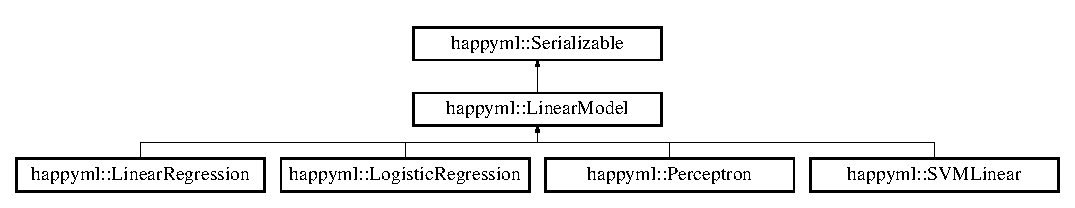
\includegraphics[height=2.346369cm]{classhappyml_1_1LinearModel}
\end{center}
\end{figure}
\subsection*{Public Member Functions}
\begin{DoxyCompactItemize}
\item 
\hyperlink{classhappyml_1_1LinearModel_a6d26af3c2b81bcd0fe08c5e23d90d5a7}{Linear\+Model} (unsigned d=0)
\begin{DoxyCompactList}\small\item\em Creates a linear model with the indicated input size. \end{DoxyCompactList}\item 
\hyperlink{classhappyml_1_1LinearModel_a6954d769ddfab54858045055a808d3dc}{Linear\+Model} (const vec \&weights)
\begin{DoxyCompactList}\small\item\em Creates a linear model with the indicated weights. \end{DoxyCompactList}\item 
\hyperlink{classhappyml_1_1LinearModel_a4670005cb3a41b6f600e4742cfbfb43c}{Linear\+Model} (const \hyperlink{classhappyml_1_1LinearModel}{Linear\+Model} \&lm)
\begin{DoxyCompactList}\small\item\em Creates a linear model from the weights of another linear model. \end{DoxyCompactList}\item 
\hyperlink{classhappyml_1_1LinearModel_a14d0bf3258e08f2f8974db865181741c}{$\sim$\+Linear\+Model} ()
\begin{DoxyCompactList}\small\item\em Destroys the linear model (sets the weights size to $0$). \end{DoxyCompactList}\item 
vec \hyperlink{classhappyml_1_1LinearModel_a22958325c41969e10fb72375eb9174a3}{get\+Weights} () const 
\begin{DoxyCompactList}\small\item\em Get a copy of the model weights. \end{DoxyCompactList}\item 
void \hyperlink{classhappyml_1_1LinearModel_abdc75a19c7234d8bc13b4dd7ad621c9e}{read} (istream \&stream)
\begin{DoxyCompactList}\small\item\em Read the weight vector from the text stream. \end{DoxyCompactList}\item 
void \hyperlink{classhappyml_1_1LinearModel_ad788fb6f13ba64d8164a89a8be96949d}{write} (ostream \&stream) const 
\begin{DoxyCompactList}\small\item\em Write the weight vector to a text stream. \end{DoxyCompactList}\end{DoxyCompactItemize}
\subsection*{Protected Attributes}
\begin{DoxyCompactItemize}
\item 
vec \hyperlink{classhappyml_1_1LinearModel_af47eec5fba48e81065101c630070a0d9}{w}
\begin{DoxyCompactList}\small\item\em Vector of weights. \end{DoxyCompactList}\end{DoxyCompactItemize}


\subsection{Detailed Description}
Hypothesis of the form $w_0 \cdot x_0 + w_1 \cdot x_1 + \cdots + w_d \cdot x_d$. 

In other words, each input feature has a weight asociated.

This class contains a protected weight vector and a public getter. 

\subsection{Constructor \& Destructor Documentation}
\index{happyml\+::\+Linear\+Model@{happyml\+::\+Linear\+Model}!Linear\+Model@{Linear\+Model}}
\index{Linear\+Model@{Linear\+Model}!happyml\+::\+Linear\+Model@{happyml\+::\+Linear\+Model}}
\subsubsection[{\texorpdfstring{Linear\+Model(unsigned d=0)}{LinearModel(unsigned d=0)}}]{\setlength{\rightskip}{0pt plus 5cm}happyml\+::\+Linear\+Model\+::\+Linear\+Model (
\begin{DoxyParamCaption}
\item[{unsigned}]{d = {\ttfamily 0}}
\end{DoxyParamCaption}
)\hspace{0.3cm}{\ttfamily [inline]}}\hypertarget{classhappyml_1_1LinearModel_a6d26af3c2b81bcd0fe08c5e23d90d5a7}{}\label{classhappyml_1_1LinearModel_a6d26af3c2b81bcd0fe08c5e23d90d5a7}


Creates a linear model with the indicated input size. 


\begin{DoxyParams}{Parameters}
{\em d} & Dimension $d$ of the input feature vectors. \\
\hline
\end{DoxyParams}
\index{happyml\+::\+Linear\+Model@{happyml\+::\+Linear\+Model}!Linear\+Model@{Linear\+Model}}
\index{Linear\+Model@{Linear\+Model}!happyml\+::\+Linear\+Model@{happyml\+::\+Linear\+Model}}
\subsubsection[{\texorpdfstring{Linear\+Model(const vec \&weights)}{LinearModel(const vec &weights)}}]{\setlength{\rightskip}{0pt plus 5cm}happyml\+::\+Linear\+Model\+::\+Linear\+Model (
\begin{DoxyParamCaption}
\item[{const vec \&}]{weights}
\end{DoxyParamCaption}
)\hspace{0.3cm}{\ttfamily [inline]}}\hypertarget{classhappyml_1_1LinearModel_a6954d769ddfab54858045055a808d3dc}{}\label{classhappyml_1_1LinearModel_a6954d769ddfab54858045055a808d3dc}


Creates a linear model with the indicated weights. 


\begin{DoxyParams}{Parameters}
{\em weights} & Weight vector with $d + 1$ dimensions. \\
\hline
\end{DoxyParams}
\index{happyml\+::\+Linear\+Model@{happyml\+::\+Linear\+Model}!Linear\+Model@{Linear\+Model}}
\index{Linear\+Model@{Linear\+Model}!happyml\+::\+Linear\+Model@{happyml\+::\+Linear\+Model}}
\subsubsection[{\texorpdfstring{Linear\+Model(const Linear\+Model \&lm)}{LinearModel(const LinearModel &lm)}}]{\setlength{\rightskip}{0pt plus 5cm}happyml\+::\+Linear\+Model\+::\+Linear\+Model (
\begin{DoxyParamCaption}
\item[{const {\bf Linear\+Model} \&}]{lm}
\end{DoxyParamCaption}
)\hspace{0.3cm}{\ttfamily [inline]}}\hypertarget{classhappyml_1_1LinearModel_a4670005cb3a41b6f600e4742cfbfb43c}{}\label{classhappyml_1_1LinearModel_a4670005cb3a41b6f600e4742cfbfb43c}


Creates a linear model from the weights of another linear model. 


\begin{DoxyParams}{Parameters}
{\em lm} & Linear model from which weights are copied. \\
\hline
\end{DoxyParams}
\index{happyml\+::\+Linear\+Model@{happyml\+::\+Linear\+Model}!````~Linear\+Model@{$\sim$\+Linear\+Model}}
\index{````~Linear\+Model@{$\sim$\+Linear\+Model}!happyml\+::\+Linear\+Model@{happyml\+::\+Linear\+Model}}
\subsubsection[{\texorpdfstring{$\sim$\+Linear\+Model()}{~LinearModel()}}]{\setlength{\rightskip}{0pt plus 5cm}happyml\+::\+Linear\+Model\+::$\sim$\+Linear\+Model (
\begin{DoxyParamCaption}
{}
\end{DoxyParamCaption}
)\hspace{0.3cm}{\ttfamily [inline]}}\hypertarget{classhappyml_1_1LinearModel_a14d0bf3258e08f2f8974db865181741c}{}\label{classhappyml_1_1LinearModel_a14d0bf3258e08f2f8974db865181741c}


Destroys the linear model (sets the weights size to $0$). 



\subsection{Member Function Documentation}
\index{happyml\+::\+Linear\+Model@{happyml\+::\+Linear\+Model}!get\+Weights@{get\+Weights}}
\index{get\+Weights@{get\+Weights}!happyml\+::\+Linear\+Model@{happyml\+::\+Linear\+Model}}
\subsubsection[{\texorpdfstring{get\+Weights() const }{getWeights() const }}]{\setlength{\rightskip}{0pt plus 5cm}vec happyml\+::\+Linear\+Model\+::get\+Weights (
\begin{DoxyParamCaption}
{}
\end{DoxyParamCaption}
) const\hspace{0.3cm}{\ttfamily [inline]}}\hypertarget{classhappyml_1_1LinearModel_a22958325c41969e10fb72375eb9174a3}{}\label{classhappyml_1_1LinearModel_a22958325c41969e10fb72375eb9174a3}


Get a copy of the model weights. 

\begin{DoxyReturn}{Returns}
Copy of the model weights. 
\end{DoxyReturn}
\index{happyml\+::\+Linear\+Model@{happyml\+::\+Linear\+Model}!read@{read}}
\index{read@{read}!happyml\+::\+Linear\+Model@{happyml\+::\+Linear\+Model}}
\subsubsection[{\texorpdfstring{read(istream \&stream)}{read(istream &stream)}}]{\setlength{\rightskip}{0pt plus 5cm}void happyml\+::\+Linear\+Model\+::read (
\begin{DoxyParamCaption}
\item[{istream \&}]{stream}
\end{DoxyParamCaption}
)\hspace{0.3cm}{\ttfamily [inline]}, {\ttfamily [virtual]}}\hypertarget{classhappyml_1_1LinearModel_abdc75a19c7234d8bc13b4dd7ad621c9e}{}\label{classhappyml_1_1LinearModel_abdc75a19c7234d8bc13b4dd7ad621c9e}


Read the weight vector from the text stream. 

Format of the stream\+: $\\ w_{0}\\ w_{1}\\ \ \ \vdots\\ w_{d} $


\begin{DoxyParams}{Parameters}
{\em stream} & Input stream. \\
\hline
\end{DoxyParams}


Implements \hyperlink{classhappyml_1_1Serializable_aef5c211d8e9c1c425b33c657824c2f0c}{happyml\+::\+Serializable}.



Reimplemented in \hyperlink{classhappyml_1_1SVMLinear_a4259c29ba1acd320703bf8c1ae8fd780}{happyml\+::\+S\+V\+M\+Linear}.

\index{happyml\+::\+Linear\+Model@{happyml\+::\+Linear\+Model}!write@{write}}
\index{write@{write}!happyml\+::\+Linear\+Model@{happyml\+::\+Linear\+Model}}
\subsubsection[{\texorpdfstring{write(ostream \&stream) const }{write(ostream &stream) const }}]{\setlength{\rightskip}{0pt plus 5cm}void happyml\+::\+Linear\+Model\+::write (
\begin{DoxyParamCaption}
\item[{ostream \&}]{stream}
\end{DoxyParamCaption}
) const\hspace{0.3cm}{\ttfamily [inline]}, {\ttfamily [virtual]}}\hypertarget{classhappyml_1_1LinearModel_ad788fb6f13ba64d8164a89a8be96949d}{}\label{classhappyml_1_1LinearModel_ad788fb6f13ba64d8164a89a8be96949d}


Write the weight vector to a text stream. 

The format of the stream will be\+: $\\ w_{0}\\ w_{1}\\ \ \ \vdots\\ w_{d} $


\begin{DoxyParams}{Parameters}
{\em stream} & Output stream. \\
\hline
\end{DoxyParams}


Implements \hyperlink{classhappyml_1_1Serializable_a2d503e4c2e39c5be8a33bcc8b691949f}{happyml\+::\+Serializable}.



\subsection{Member Data Documentation}
\index{happyml\+::\+Linear\+Model@{happyml\+::\+Linear\+Model}!w@{w}}
\index{w@{w}!happyml\+::\+Linear\+Model@{happyml\+::\+Linear\+Model}}
\subsubsection[{\texorpdfstring{w}{w}}]{\setlength{\rightskip}{0pt plus 5cm}vec happyml\+::\+Linear\+Model\+::w\hspace{0.3cm}{\ttfamily [protected]}}\hypertarget{classhappyml_1_1LinearModel_af47eec5fba48e81065101c630070a0d9}{}\label{classhappyml_1_1LinearModel_af47eec5fba48e81065101c630070a0d9}


Vector of weights. 



The documentation for this class was generated from the following file\+:\begin{DoxyCompactItemize}
\item 
include/happyml/\hyperlink{linear__model_8h}{linear\+\_\+model.\+h}\end{DoxyCompactItemize}

\hypertarget{classhappyml_1_1LinearRegression}{}\section{happyml\+:\+:Linear\+Regression Class Reference}
\label{classhappyml_1_1LinearRegression}\index{happyml\+::\+Linear\+Regression@{happyml\+::\+Linear\+Regression}}


{\ttfamily \#include $<$linear\+\_\+regression.\+h$>$}

Inheritance diagram for happyml\+:\+:Linear\+Regression\+:\begin{figure}[H]
\begin{center}
\leavevmode
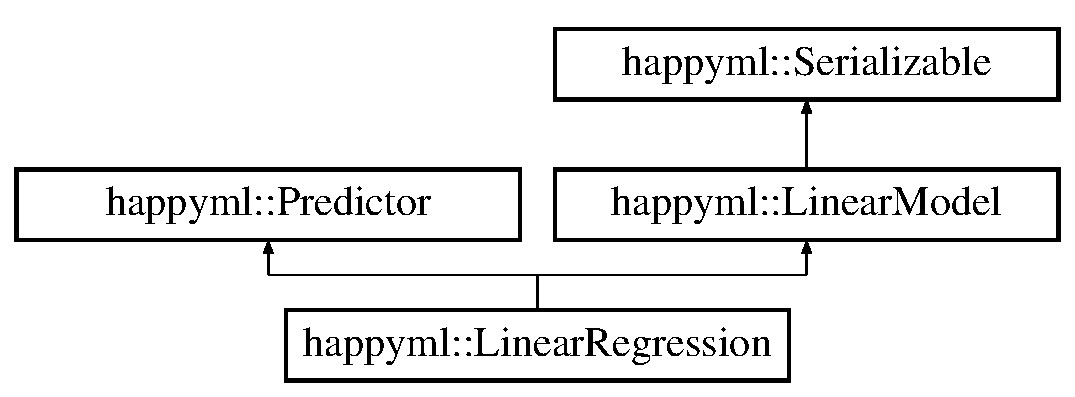
\includegraphics[height=3.000000cm]{classhappyml_1_1LinearRegression}
\end{center}
\end{figure}
\subsection*{Public Member Functions}
\begin{DoxyCompactItemize}
\item 
\hyperlink{classhappyml_1_1LinearRegression_aec943f0f85a5a99f41439b54ea2ac473}{Linear\+Regression} (unsigned d=0)
\begin{DoxyCompactList}\small\item\em Creates a linear regression algorithm with the indicated input size. \end{DoxyCompactList}\item 
\hyperlink{classhappyml_1_1LinearRegression_a1679264b5b2c992256cd3a8c1f98b02c}{Linear\+Regression} (const vec \&weights)
\begin{DoxyCompactList}\small\item\em Creates a linear regression algorithm with the indicated weights. \end{DoxyCompactList}\item 
\hyperlink{classhappyml_1_1LinearRegression_ac23946a5699a2f9ce5853e5e2ad10a4b}{Linear\+Regression} (const \hyperlink{classhappyml_1_1LinearModel}{Linear\+Model} \&lm)
\item 
double \hyperlink{classhappyml_1_1LinearRegression_a49a96b35d3f85a7ebd78fcc61c21f83e}{train} (const \hyperlink{classhappyml_1_1DataSet}{Data\+Set} \&data)
\begin{DoxyCompactList}\small\item\em Train the linear regression. \end{DoxyCompactList}\item 
double \hyperlink{classhappyml_1_1LinearRegression_ae707c7931a3be6d33108a34cdbb05422}{train} (const \hyperlink{classhappyml_1_1DataSet}{Data\+Set} \&data, double lambda)
\begin{DoxyCompactList}\small\item\em Train the linear regression. \end{DoxyCompactList}\item 
double \hyperlink{classhappyml_1_1LinearRegression_af7b493c394ab2664c5e743711a64d26e}{predict} (const \hyperlink{namespacehappyml_a03602d1ec49393790b8a0449f40cd01f}{Input} \&x) const 
\begin{DoxyCompactList}\small\item\em Predict the output of an input vector. \end{DoxyCompactList}\item 
double \hyperlink{classhappyml_1_1LinearRegression_aebb84fbdbfed7487c05baa8d8c1499e9}{error} (const \hyperlink{classhappyml_1_1DataSet}{Data\+Set} \&data) const 
\begin{DoxyCompactList}\small\item\em Compute the mean squared error of the linear regression algorithm on the given dataset. \end{DoxyCompactList}\end{DoxyCompactItemize}
\subsection*{Additional Inherited Members}


\subsection{Constructor \& Destructor Documentation}
\index{happyml\+::\+Linear\+Regression@{happyml\+::\+Linear\+Regression}!Linear\+Regression@{Linear\+Regression}}
\index{Linear\+Regression@{Linear\+Regression}!happyml\+::\+Linear\+Regression@{happyml\+::\+Linear\+Regression}}
\subsubsection[{\texorpdfstring{Linear\+Regression(unsigned d=0)}{LinearRegression(unsigned d=0)}}]{\setlength{\rightskip}{0pt plus 5cm}happyml\+::\+Linear\+Regression\+::\+Linear\+Regression (
\begin{DoxyParamCaption}
\item[{unsigned}]{d = {\ttfamily 0}}
\end{DoxyParamCaption}
)\hspace{0.3cm}{\ttfamily [inline]}}\hypertarget{classhappyml_1_1LinearRegression_aec943f0f85a5a99f41439b54ea2ac473}{}\label{classhappyml_1_1LinearRegression_aec943f0f85a5a99f41439b54ea2ac473}


Creates a linear regression algorithm with the indicated input size. 


\begin{DoxyParams}{Parameters}
{\em d} & Dimension $d$, number of features of the input vectors. \\
\hline
\end{DoxyParams}
\index{happyml\+::\+Linear\+Regression@{happyml\+::\+Linear\+Regression}!Linear\+Regression@{Linear\+Regression}}
\index{Linear\+Regression@{Linear\+Regression}!happyml\+::\+Linear\+Regression@{happyml\+::\+Linear\+Regression}}
\subsubsection[{\texorpdfstring{Linear\+Regression(const vec \&weights)}{LinearRegression(const vec &weights)}}]{\setlength{\rightskip}{0pt plus 5cm}happyml\+::\+Linear\+Regression\+::\+Linear\+Regression (
\begin{DoxyParamCaption}
\item[{const vec \&}]{weights}
\end{DoxyParamCaption}
)\hspace{0.3cm}{\ttfamily [inline]}}\hypertarget{classhappyml_1_1LinearRegression_a1679264b5b2c992256cd3a8c1f98b02c}{}\label{classhappyml_1_1LinearRegression_a1679264b5b2c992256cd3a8c1f98b02c}


Creates a linear regression algorithm with the indicated weights. 


\begin{DoxyParams}{Parameters}
{\em weights} & Weight vector with $d + 1$ size. \\
\hline
\end{DoxyParams}
\index{happyml\+::\+Linear\+Regression@{happyml\+::\+Linear\+Regression}!Linear\+Regression@{Linear\+Regression}}
\index{Linear\+Regression@{Linear\+Regression}!happyml\+::\+Linear\+Regression@{happyml\+::\+Linear\+Regression}}
\subsubsection[{\texorpdfstring{Linear\+Regression(const Linear\+Model \&lm)}{LinearRegression(const LinearModel &lm)}}]{\setlength{\rightskip}{0pt plus 5cm}happyml\+::\+Linear\+Regression\+::\+Linear\+Regression (
\begin{DoxyParamCaption}
\item[{const {\bf Linear\+Model} \&}]{lm}
\end{DoxyParamCaption}
)\hspace{0.3cm}{\ttfamily [inline]}}\hypertarget{classhappyml_1_1LinearRegression_ac23946a5699a2f9ce5853e5e2ad10a4b}{}\label{classhappyml_1_1LinearRegression_ac23946a5699a2f9ce5853e5e2ad10a4b}


\subsection{Member Function Documentation}
\index{happyml\+::\+Linear\+Regression@{happyml\+::\+Linear\+Regression}!error@{error}}
\index{error@{error}!happyml\+::\+Linear\+Regression@{happyml\+::\+Linear\+Regression}}
\subsubsection[{\texorpdfstring{error(const Data\+Set \&data) const }{error(const DataSet &data) const }}]{\setlength{\rightskip}{0pt plus 5cm}double happyml\+::\+Linear\+Regression\+::error (
\begin{DoxyParamCaption}
\item[{const {\bf Data\+Set} \&}]{data}
\end{DoxyParamCaption}
) const\hspace{0.3cm}{\ttfamily [virtual]}}\hypertarget{classhappyml_1_1LinearRegression_aebb84fbdbfed7487c05baa8d8c1499e9}{}\label{classhappyml_1_1LinearRegression_aebb84fbdbfed7487c05baa8d8c1499e9}


Compute the mean squared error of the linear regression algorithm on the given dataset. 


\begin{DoxyParams}{Parameters}
{\em data} & Dataset with the correct output.\\
\hline
\end{DoxyParams}
\begin{DoxyReturn}{Returns}
Error of classify the given dataset. It\textquotesingle{}s value is grater than $0$. 
\end{DoxyReturn}


Reimplemented from \hyperlink{classhappyml_1_1Predictor_a59b022fac2ffa3a0254b75cb02b70dfe}{happyml\+::\+Predictor}.

\index{happyml\+::\+Linear\+Regression@{happyml\+::\+Linear\+Regression}!predict@{predict}}
\index{predict@{predict}!happyml\+::\+Linear\+Regression@{happyml\+::\+Linear\+Regression}}
\subsubsection[{\texorpdfstring{predict(const Input \&x) const }{predict(const Input &x) const }}]{\setlength{\rightskip}{0pt plus 5cm}double happyml\+::\+Linear\+Regression\+::predict (
\begin{DoxyParamCaption}
\item[{const {\bf Input} \&}]{x}
\end{DoxyParamCaption}
) const\hspace{0.3cm}{\ttfamily [virtual]}}\hypertarget{classhappyml_1_1LinearRegression_af7b493c394ab2664c5e743711a64d26e}{}\label{classhappyml_1_1LinearRegression_af7b493c394ab2664c5e743711a64d26e}


Predict the output of an input vector. 

\begin{DoxyReturn}{Returns}
Estimated real output. 
\end{DoxyReturn}


Implements \hyperlink{classhappyml_1_1Predictor_a07cf89d655e7642fd94c9b2a8fd0a04b}{happyml\+::\+Predictor}.

\index{happyml\+::\+Linear\+Regression@{happyml\+::\+Linear\+Regression}!train@{train}}
\index{train@{train}!happyml\+::\+Linear\+Regression@{happyml\+::\+Linear\+Regression}}
\subsubsection[{\texorpdfstring{train(const Data\+Set \&data)}{train(const DataSet &data)}}]{\setlength{\rightskip}{0pt plus 5cm}double happyml\+::\+Linear\+Regression\+::train (
\begin{DoxyParamCaption}
\item[{const {\bf Data\+Set} \&}]{data}
\end{DoxyParamCaption}
)}\hypertarget{classhappyml_1_1LinearRegression_a49a96b35d3f85a7ebd78fcc61c21f83e}{}\label{classhappyml_1_1LinearRegression_a49a96b35d3f85a7ebd78fcc61c21f83e}


Train the linear regression. 


\begin{DoxyParams}{Parameters}
{\em data} & Training set.\\
\hline
\end{DoxyParams}
\begin{DoxyReturn}{Returns}
Returns the final error. 
\end{DoxyReturn}
\index{happyml\+::\+Linear\+Regression@{happyml\+::\+Linear\+Regression}!train@{train}}
\index{train@{train}!happyml\+::\+Linear\+Regression@{happyml\+::\+Linear\+Regression}}
\subsubsection[{\texorpdfstring{train(const Data\+Set \&data, double lambda)}{train(const DataSet &data, double lambda)}}]{\setlength{\rightskip}{0pt plus 5cm}double happyml\+::\+Linear\+Regression\+::train (
\begin{DoxyParamCaption}
\item[{const {\bf Data\+Set} \&}]{data, }
\item[{double}]{lambda}
\end{DoxyParamCaption}
)}\hypertarget{classhappyml_1_1LinearRegression_ae707c7931a3be6d33108a34cdbb05422}{}\label{classhappyml_1_1LinearRegression_ae707c7931a3be6d33108a34cdbb05422}


Train the linear regression. 


\begin{DoxyParams}{Parameters}
{\em data} & Training set. \\
\hline
{\em lambda} & Regularization paramiter $\lambda$.\\
\hline
\end{DoxyParams}
\begin{DoxyReturn}{Returns}
Returns the final error. 
\end{DoxyReturn}


The documentation for this class was generated from the following files\+:\begin{DoxyCompactItemize}
\item 
include/happyml/linear\+\_\+regression/\hyperlink{linear__regression_8h}{linear\+\_\+regression.\+h}\item 
src/linear\+\_\+regression/\hyperlink{linear__regression_8cpp}{linear\+\_\+regression.\+cpp}\end{DoxyCompactItemize}

\hypertarget{classhappyml_1_1LogisticRegression}{}\section{happyml\+:\+:Logistic\+Regression Class Reference}
\label{classhappyml_1_1LogisticRegression}\index{happyml\+::\+Logistic\+Regression@{happyml\+::\+Logistic\+Regression}}


{\ttfamily \#include $<$logistic\+\_\+regression.\+h$>$}

Inheritance diagram for happyml\+:\+:Logistic\+Regression\+:\begin{figure}[H]
\begin{center}
\leavevmode
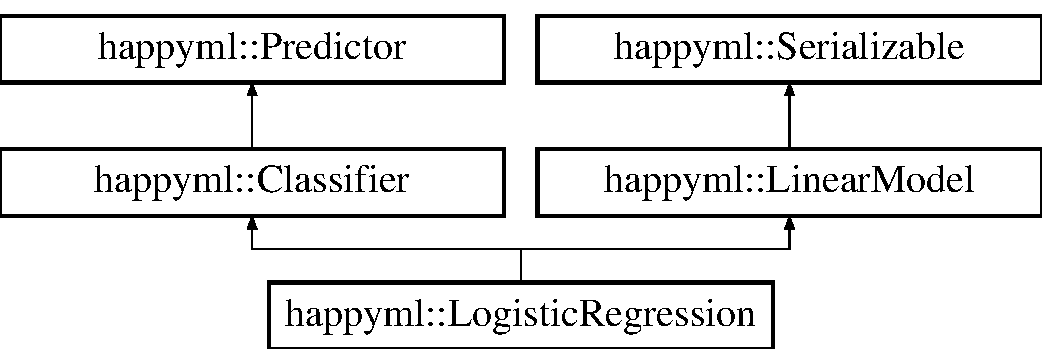
\includegraphics[height=3.000000cm]{classhappyml_1_1LogisticRegression}
\end{center}
\end{figure}
\subsection*{Public Member Functions}
\begin{DoxyCompactItemize}
\item 
\hyperlink{classhappyml_1_1LogisticRegression_ab3f409e0e3d6c0e95bba0bd86db953ae}{Logistic\+Regression} (unsigned d=0)
\begin{DoxyCompactList}\small\item\em Creates a logistic regression algorithm with the indicated input size. \end{DoxyCompactList}\item 
\hyperlink{classhappyml_1_1LogisticRegression_a42c6f431670db4fea1aff55b3b0cb034}{Logistic\+Regression} (const vec \&weights)
\begin{DoxyCompactList}\small\item\em Creates a logistic regression algorithm with the indicated weights. \end{DoxyCompactList}\item 
\hyperlink{classhappyml_1_1LogisticRegression_afe828c9c1370632d47df5eb0fbc2fe1a}{Logistic\+Regression} (const \hyperlink{classhappyml_1_1LinearModel}{Linear\+Model} \&lm)
\item 
double \hyperlink{classhappyml_1_1LogisticRegression_ae997703343acb56b827ea257775cc971}{train} (const \hyperlink{classhappyml_1_1DataSet}{Data\+Set} \&data, unsigned iter=1000, double learning\+\_\+rate=0.\+1)
\begin{DoxyCompactList}\small\item\em Train the logistic regression until the training loops over the data n\+Times, or classifies all correctly. \end{DoxyCompactList}\item 
double \hyperlink{classhappyml_1_1LogisticRegression_abd9bb137ef99e360fcffcca3187b6703}{predict} (const \hyperlink{namespacehappyml_a03602d1ec49393790b8a0449f40cd01f}{Input} \&x) const 
\begin{DoxyCompactList}\small\item\em Classifies an input vector. \end{DoxyCompactList}\item 
double \hyperlink{classhappyml_1_1LogisticRegression_a40140d6f83cae49ad1472bcf8678da15}{error} (const \hyperlink{classhappyml_1_1DataSet}{Data\+Set} \&data) const 
\begin{DoxyCompactList}\small\item\em Compute the error of the logistic regression on the given dataset. \end{DoxyCompactList}\end{DoxyCompactItemize}
\subsection*{Additional Inherited Members}


\subsection{Constructor \& Destructor Documentation}
\index{happyml\+::\+Logistic\+Regression@{happyml\+::\+Logistic\+Regression}!Logistic\+Regression@{Logistic\+Regression}}
\index{Logistic\+Regression@{Logistic\+Regression}!happyml\+::\+Logistic\+Regression@{happyml\+::\+Logistic\+Regression}}
\subsubsection[{\texorpdfstring{Logistic\+Regression(unsigned d=0)}{LogisticRegression(unsigned d=0)}}]{\setlength{\rightskip}{0pt plus 5cm}happyml\+::\+Logistic\+Regression\+::\+Logistic\+Regression (
\begin{DoxyParamCaption}
\item[{unsigned}]{d = {\ttfamily 0}}
\end{DoxyParamCaption}
)\hspace{0.3cm}{\ttfamily [inline]}}\hypertarget{classhappyml_1_1LogisticRegression_ab3f409e0e3d6c0e95bba0bd86db953ae}{}\label{classhappyml_1_1LogisticRegression_ab3f409e0e3d6c0e95bba0bd86db953ae}


Creates a logistic regression algorithm with the indicated input size. 


\begin{DoxyParams}{Parameters}
{\em d} & Dimension $d$ of the input feature vectors. \\
\hline
\end{DoxyParams}
\index{happyml\+::\+Logistic\+Regression@{happyml\+::\+Logistic\+Regression}!Logistic\+Regression@{Logistic\+Regression}}
\index{Logistic\+Regression@{Logistic\+Regression}!happyml\+::\+Logistic\+Regression@{happyml\+::\+Logistic\+Regression}}
\subsubsection[{\texorpdfstring{Logistic\+Regression(const vec \&weights)}{LogisticRegression(const vec &weights)}}]{\setlength{\rightskip}{0pt plus 5cm}happyml\+::\+Logistic\+Regression\+::\+Logistic\+Regression (
\begin{DoxyParamCaption}
\item[{const vec \&}]{weights}
\end{DoxyParamCaption}
)\hspace{0.3cm}{\ttfamily [inline]}}\hypertarget{classhappyml_1_1LogisticRegression_a42c6f431670db4fea1aff55b3b0cb034}{}\label{classhappyml_1_1LogisticRegression_a42c6f431670db4fea1aff55b3b0cb034}


Creates a logistic regression algorithm with the indicated weights. 


\begin{DoxyParams}{Parameters}
{\em weights} & Weight vector with $d + 1$ size. \\
\hline
\end{DoxyParams}
\index{happyml\+::\+Logistic\+Regression@{happyml\+::\+Logistic\+Regression}!Logistic\+Regression@{Logistic\+Regression}}
\index{Logistic\+Regression@{Logistic\+Regression}!happyml\+::\+Logistic\+Regression@{happyml\+::\+Logistic\+Regression}}
\subsubsection[{\texorpdfstring{Logistic\+Regression(const Linear\+Model \&lm)}{LogisticRegression(const LinearModel &lm)}}]{\setlength{\rightskip}{0pt plus 5cm}happyml\+::\+Logistic\+Regression\+::\+Logistic\+Regression (
\begin{DoxyParamCaption}
\item[{const {\bf Linear\+Model} \&}]{lm}
\end{DoxyParamCaption}
)\hspace{0.3cm}{\ttfamily [inline]}}\hypertarget{classhappyml_1_1LogisticRegression_afe828c9c1370632d47df5eb0fbc2fe1a}{}\label{classhappyml_1_1LogisticRegression_afe828c9c1370632d47df5eb0fbc2fe1a}


\subsection{Member Function Documentation}
\index{happyml\+::\+Logistic\+Regression@{happyml\+::\+Logistic\+Regression}!error@{error}}
\index{error@{error}!happyml\+::\+Logistic\+Regression@{happyml\+::\+Logistic\+Regression}}
\subsubsection[{\texorpdfstring{error(const Data\+Set \&data) const }{error(const DataSet &data) const }}]{\setlength{\rightskip}{0pt plus 5cm}double happyml\+::\+Logistic\+Regression\+::error (
\begin{DoxyParamCaption}
\item[{const {\bf Data\+Set} \&}]{data}
\end{DoxyParamCaption}
) const\hspace{0.3cm}{\ttfamily [virtual]}}\hypertarget{classhappyml_1_1LogisticRegression_a40140d6f83cae49ad1472bcf8678da15}{}\label{classhappyml_1_1LogisticRegression_a40140d6f83cae49ad1472bcf8678da15}


Compute the error of the logistic regression on the given dataset. 


\begin{DoxyParams}{Parameters}
{\em data} & Dataset with the correct output.\\
\hline
\end{DoxyParams}
\begin{DoxyReturn}{Returns}
Error of classify the given dataset. It\textquotesingle{}s value is grater than $0$. 
\end{DoxyReturn}


Reimplemented from \hyperlink{classhappyml_1_1Predictor_a59b022fac2ffa3a0254b75cb02b70dfe}{happyml\+::\+Predictor}.

\index{happyml\+::\+Logistic\+Regression@{happyml\+::\+Logistic\+Regression}!predict@{predict}}
\index{predict@{predict}!happyml\+::\+Logistic\+Regression@{happyml\+::\+Logistic\+Regression}}
\subsubsection[{\texorpdfstring{predict(const Input \&x) const }{predict(const Input &x) const }}]{\setlength{\rightskip}{0pt plus 5cm}double happyml\+::\+Logistic\+Regression\+::predict (
\begin{DoxyParamCaption}
\item[{const {\bf Input} \&}]{x}
\end{DoxyParamCaption}
) const\hspace{0.3cm}{\ttfamily [virtual]}}\hypertarget{classhappyml_1_1LogisticRegression_abd9bb137ef99e360fcffcca3187b6703}{}\label{classhappyml_1_1LogisticRegression_abd9bb137ef99e360fcffcca3187b6703}


Classifies an input vector. 

\begin{DoxyReturn}{Returns}
Probability of the input to belong to +1 class. Output in the interval $[0, 1]$. 
\end{DoxyReturn}


Implements \hyperlink{classhappyml_1_1Predictor_a07cf89d655e7642fd94c9b2a8fd0a04b}{happyml\+::\+Predictor}.

\index{happyml\+::\+Logistic\+Regression@{happyml\+::\+Logistic\+Regression}!train@{train}}
\index{train@{train}!happyml\+::\+Logistic\+Regression@{happyml\+::\+Logistic\+Regression}}
\subsubsection[{\texorpdfstring{train(const Data\+Set \&data, unsigned iter=1000, double learning\+\_\+rate=0.\+1)}{train(const DataSet &data, unsigned iter=1000, double learning_rate=0.1)}}]{\setlength{\rightskip}{0pt plus 5cm}double happyml\+::\+Logistic\+Regression\+::train (
\begin{DoxyParamCaption}
\item[{const {\bf Data\+Set} \&}]{data, }
\item[{unsigned}]{iter = {\ttfamily 1000}, }
\item[{double}]{learning\+\_\+rate = {\ttfamily 0.1}}
\end{DoxyParamCaption}
)}\hypertarget{classhappyml_1_1LogisticRegression_ae997703343acb56b827ea257775cc971}{}\label{classhappyml_1_1LogisticRegression_ae997703343acb56b827ea257775cc971}


Train the logistic regression until the training loops over the data n\+Times, or classifies all correctly. 

Data must contain the $x_0 = 1$ property.


\begin{DoxyParams}{Parameters}
{\em data} & Training set. \\
\hline
{\em iter} & Maximun number of iterations ( $1000$ by default). \\
\hline
{\em learning\+\_\+rate} & Learning rate ( $0.1$ by default.).\\
\hline
\end{DoxyParams}
\begin{DoxyReturn}{Returns}
Returns the error of the best weights found. 
\end{DoxyReturn}


The documentation for this class was generated from the following files\+:\begin{DoxyCompactItemize}
\item 
include/happyml/logistic\+\_\+regression/\hyperlink{logistic__regression_8h}{logistic\+\_\+regression.\+h}\item 
src/logistic\+\_\+regression/\hyperlink{logistic__regression_8cpp}{logistic\+\_\+regression.\+cpp}\end{DoxyCompactItemize}

\hypertarget{classhappyml_1_1transforms_1_1Mul}{}\section{happyml\+:\+:transforms\+:\+:Mul Class Reference}
\label{classhappyml_1_1transforms_1_1Mul}\index{happyml\+::transforms\+::\+Mul@{happyml\+::transforms\+::\+Mul}}


{\ttfamily \#include $<$transformer.\+h$>$}

Inheritance diagram for happyml\+:\+:transforms\+:\+:Mul\+:\begin{figure}[H]
\begin{center}
\leavevmode
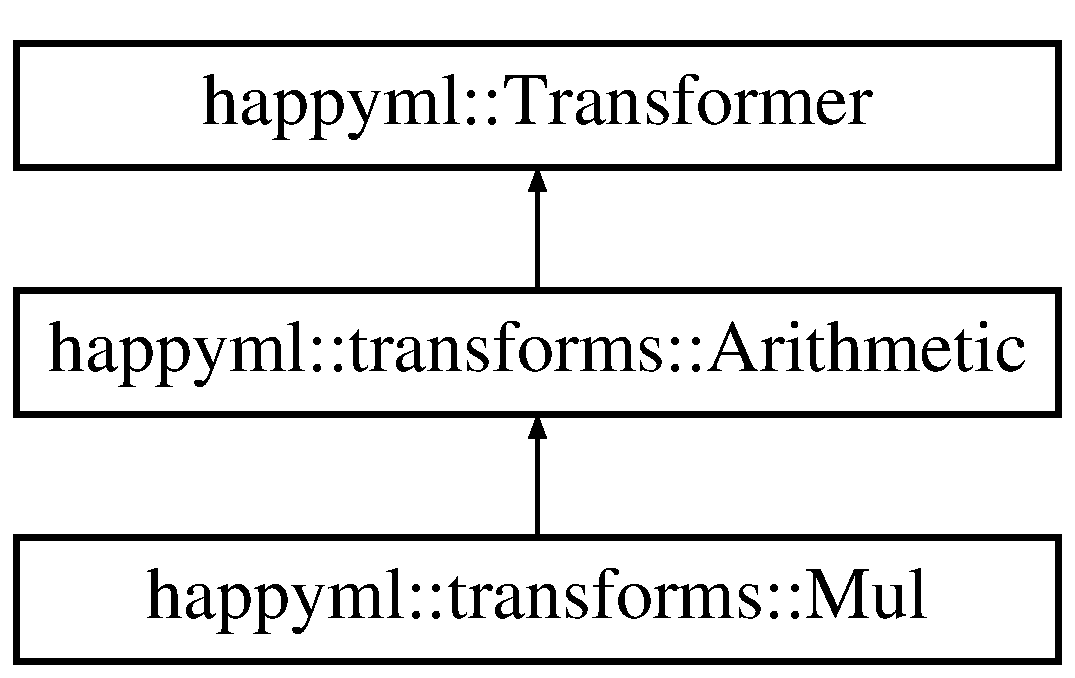
\includegraphics[height=3.000000cm]{classhappyml_1_1transforms_1_1Mul}
\end{center}
\end{figure}
\subsection*{Public Member Functions}
\begin{DoxyCompactItemize}
\item 
\hyperlink{classhappyml_1_1transforms_1_1Mul_a787cee14f1004aac475e52058c9ed6be}{Mul} (int f, double p, bool nf=false)
\item 
void \hyperlink{classhappyml_1_1transforms_1_1Mul_afc91c3f53e31af40b314cc0d9d5552fa}{apply} (mat \&x, int col) const 
\end{DoxyCompactItemize}
\subsection*{Additional Inherited Members}


\subsection{Constructor \& Destructor Documentation}
\index{happyml\+::transforms\+::\+Mul@{happyml\+::transforms\+::\+Mul}!Mul@{Mul}}
\index{Mul@{Mul}!happyml\+::transforms\+::\+Mul@{happyml\+::transforms\+::\+Mul}}
\subsubsection[{\texorpdfstring{Mul(int f, double p, bool nf=false)}{Mul(int f, double p, bool nf=false)}}]{\setlength{\rightskip}{0pt plus 5cm}happyml\+::transforms\+::\+Mul\+::\+Mul (
\begin{DoxyParamCaption}
\item[{int}]{f, }
\item[{double}]{p, }
\item[{bool}]{nf = {\ttfamily false}}
\end{DoxyParamCaption}
)\hspace{0.3cm}{\ttfamily [inline]}}\hypertarget{classhappyml_1_1transforms_1_1Mul_a787cee14f1004aac475e52058c9ed6be}{}\label{classhappyml_1_1transforms_1_1Mul_a787cee14f1004aac475e52058c9ed6be}


\subsection{Member Function Documentation}
\index{happyml\+::transforms\+::\+Mul@{happyml\+::transforms\+::\+Mul}!apply@{apply}}
\index{apply@{apply}!happyml\+::transforms\+::\+Mul@{happyml\+::transforms\+::\+Mul}}
\subsubsection[{\texorpdfstring{apply(mat \&x, int col) const }{apply(mat &x, int col) const }}]{\setlength{\rightskip}{0pt plus 5cm}void happyml\+::transforms\+::\+Mul\+::apply (
\begin{DoxyParamCaption}
\item[{mat \&}]{x, }
\item[{int}]{col}
\end{DoxyParamCaption}
) const\hspace{0.3cm}{\ttfamily [virtual]}}\hypertarget{classhappyml_1_1transforms_1_1Mul_afc91c3f53e31af40b314cc0d9d5552fa}{}\label{classhappyml_1_1transforms_1_1Mul_afc91c3f53e31af40b314cc0d9d5552fa}


Implements \hyperlink{classhappyml_1_1transforms_1_1Arithmetic_a85191dcd8734e18424b92b870d7b9d73}{happyml\+::transforms\+::\+Arithmetic}.



The documentation for this class was generated from the following files\+:\begin{DoxyCompactItemize}
\item 
include/happyml/transformers/\hyperlink{transformer_8h}{transformer.\+h}\item 
src/transformers/\hyperlink{transformer_8cpp}{transformer.\+cpp}\end{DoxyCompactItemize}

\hypertarget{classhappyml_1_1NeuralNetwork}{}\section{happyml\+:\+:Neural\+Network Class Reference}
\label{classhappyml_1_1NeuralNetwork}\index{happyml\+::\+Neural\+Network@{happyml\+::\+Neural\+Network}}


{\ttfamily \#include $<$neural\+\_\+network.\+h$>$}

Inheritance diagram for happyml\+:\+:Neural\+Network\+:\begin{figure}[H]
\begin{center}
\leavevmode
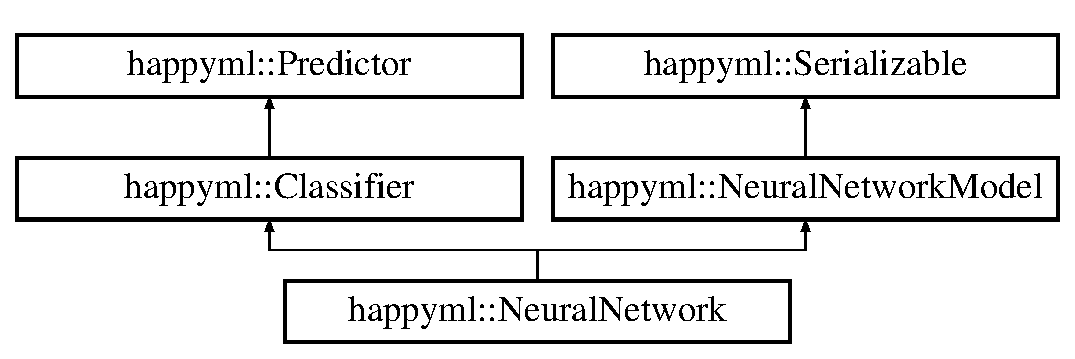
\includegraphics[height=3.000000cm]{classhappyml_1_1NeuralNetwork}
\end{center}
\end{figure}
\subsection*{Public Member Functions}
\begin{DoxyCompactItemize}
\item 
\hyperlink{classhappyml_1_1NeuralNetwork_ab99bc065c560df1c116cc1eb26480f56}{Neural\+Network} (unsigned layers=0...)
\item 
\hyperlink{classhappyml_1_1NeuralNetwork_addf2c3d3d29a69a83876fd200a75d7ed}{Neural\+Network} (const vector$<$ unsigned $>$ \&layers)
\item 
\hyperlink{classhappyml_1_1NeuralNetwork_ae82d4d36bf87fbeaede4b7fcd8c3afd1}{Neural\+Network} (const vector$<$ mat $>$ w)
\item 
\hyperlink{classhappyml_1_1NeuralNetwork_a69f0a4cfa957f6a0b7cf669831939456}{Neural\+Network} (const \hyperlink{classhappyml_1_1NeuralNetwork}{Neural\+Network} \&nn)
\item 
\hyperlink{classhappyml_1_1NeuralNetwork_a4db646511b7f539b1f6e26220b7c9192}{$\sim$\+Neural\+Network} ()
\item 
double \hyperlink{classhappyml_1_1NeuralNetwork_a90aca4a568024edfd8c325b8f5aa5b74}{train} (const \hyperlink{classhappyml_1_1DataSet}{Data\+Set} \&dataset, unsigned iter=500, float learning\+\_\+rate=0.\+1, float lambda=0, float delta\+\_\+stop=-\/1)
\begin{DoxyCompactList}\small\item\em Train the neural network until the training loops over the data iter times. \end{DoxyCompactList}\item 
double \hyperlink{classhappyml_1_1NeuralNetwork_afd27297d91418b40ca7a943f313a4902}{sgd\+Train} (const \hyperlink{classhappyml_1_1DataSet}{Data\+Set} \&dataset, unsigned iter=500, float learning\+\_\+rate=0.\+1, float lambda=0, int batch\+\_\+size=32)
\item 
double \hyperlink{classhappyml_1_1NeuralNetwork_ae2e05acd3a864d20ca1a1645c1e369e4}{predict} (const \hyperlink{namespacehappyml_a03602d1ec49393790b8a0449f40cd01f}{Input} \&x) const 
\begin{DoxyCompactList}\small\item\em Uses the forward propagation algorithm to predict an output. \end{DoxyCompactList}\item 
vec \hyperlink{classhappyml_1_1NeuralNetwork_af4e1fbe2ef96f8a08b11dc9b9f0f7230}{predict\+Vec} (const \hyperlink{namespacehappyml_a03602d1ec49393790b8a0449f40cd01f}{Input} \&x) const 
\item 
double \hyperlink{classhappyml_1_1NeuralNetwork_a5653b6fb601bcb410aa9ff84611e428d}{get\+Last\+Iterations} () const 
\begin{DoxyCompactList}\small\item\em Returns the number of iterations performed in last training. \end{DoxyCompactList}\end{DoxyCompactItemize}
\subsection*{Protected Attributes}
\begin{DoxyCompactItemize}
\item 
unsigned \hyperlink{classhappyml_1_1NeuralNetwork_a87469b54a244913da3c4f39e4d99abdd}{last\+Iterations}
\end{DoxyCompactItemize}
\subsection*{Additional Inherited Members}


\subsection{Constructor \& Destructor Documentation}
\index{happyml\+::\+Neural\+Network@{happyml\+::\+Neural\+Network}!Neural\+Network@{Neural\+Network}}
\index{Neural\+Network@{Neural\+Network}!happyml\+::\+Neural\+Network@{happyml\+::\+Neural\+Network}}
\subsubsection[{\texorpdfstring{Neural\+Network(unsigned layers=0...)}{NeuralNetwork(unsigned layers=0...)}}]{\setlength{\rightskip}{0pt plus 5cm}happyml\+::\+Neural\+Network\+::\+Neural\+Network (
\begin{DoxyParamCaption}
\item[{unsigned}]{layers = {\ttfamily 0...}}
\end{DoxyParamCaption}
)}\hypertarget{classhappyml_1_1NeuralNetwork_ab99bc065c560df1c116cc1eb26480f56}{}\label{classhappyml_1_1NeuralNetwork_ab99bc065c560df1c116cc1eb26480f56}
\index{happyml\+::\+Neural\+Network@{happyml\+::\+Neural\+Network}!Neural\+Network@{Neural\+Network}}
\index{Neural\+Network@{Neural\+Network}!happyml\+::\+Neural\+Network@{happyml\+::\+Neural\+Network}}
\subsubsection[{\texorpdfstring{Neural\+Network(const vector$<$ unsigned $>$ \&layers)}{NeuralNetwork(const vector< unsigned > &layers)}}]{\setlength{\rightskip}{0pt plus 5cm}happyml\+::\+Neural\+Network\+::\+Neural\+Network (
\begin{DoxyParamCaption}
\item[{const vector$<$ unsigned $>$ \&}]{layers}
\end{DoxyParamCaption}
)\hspace{0.3cm}{\ttfamily [inline]}}\hypertarget{classhappyml_1_1NeuralNetwork_addf2c3d3d29a69a83876fd200a75d7ed}{}\label{classhappyml_1_1NeuralNetwork_addf2c3d3d29a69a83876fd200a75d7ed}
\index{happyml\+::\+Neural\+Network@{happyml\+::\+Neural\+Network}!Neural\+Network@{Neural\+Network}}
\index{Neural\+Network@{Neural\+Network}!happyml\+::\+Neural\+Network@{happyml\+::\+Neural\+Network}}
\subsubsection[{\texorpdfstring{Neural\+Network(const vector$<$ mat $>$ w)}{NeuralNetwork(const vector< mat > w)}}]{\setlength{\rightskip}{0pt plus 5cm}happyml\+::\+Neural\+Network\+::\+Neural\+Network (
\begin{DoxyParamCaption}
\item[{const vector$<$ mat $>$}]{w}
\end{DoxyParamCaption}
)\hspace{0.3cm}{\ttfamily [inline]}}\hypertarget{classhappyml_1_1NeuralNetwork_ae82d4d36bf87fbeaede4b7fcd8c3afd1}{}\label{classhappyml_1_1NeuralNetwork_ae82d4d36bf87fbeaede4b7fcd8c3afd1}
\index{happyml\+::\+Neural\+Network@{happyml\+::\+Neural\+Network}!Neural\+Network@{Neural\+Network}}
\index{Neural\+Network@{Neural\+Network}!happyml\+::\+Neural\+Network@{happyml\+::\+Neural\+Network}}
\subsubsection[{\texorpdfstring{Neural\+Network(const Neural\+Network \&nn)}{NeuralNetwork(const NeuralNetwork &nn)}}]{\setlength{\rightskip}{0pt plus 5cm}happyml\+::\+Neural\+Network\+::\+Neural\+Network (
\begin{DoxyParamCaption}
\item[{const {\bf Neural\+Network} \&}]{nn}
\end{DoxyParamCaption}
)\hspace{0.3cm}{\ttfamily [inline]}}\hypertarget{classhappyml_1_1NeuralNetwork_a69f0a4cfa957f6a0b7cf669831939456}{}\label{classhappyml_1_1NeuralNetwork_a69f0a4cfa957f6a0b7cf669831939456}
\index{happyml\+::\+Neural\+Network@{happyml\+::\+Neural\+Network}!````~Neural\+Network@{$\sim$\+Neural\+Network}}
\index{````~Neural\+Network@{$\sim$\+Neural\+Network}!happyml\+::\+Neural\+Network@{happyml\+::\+Neural\+Network}}
\subsubsection[{\texorpdfstring{$\sim$\+Neural\+Network()}{~NeuralNetwork()}}]{\setlength{\rightskip}{0pt plus 5cm}happyml\+::\+Neural\+Network\+::$\sim$\+Neural\+Network (
\begin{DoxyParamCaption}
{}
\end{DoxyParamCaption}
)\hspace{0.3cm}{\ttfamily [inline]}}\hypertarget{classhappyml_1_1NeuralNetwork_a4db646511b7f539b1f6e26220b7c9192}{}\label{classhappyml_1_1NeuralNetwork_a4db646511b7f539b1f6e26220b7c9192}


\subsection{Member Function Documentation}
\index{happyml\+::\+Neural\+Network@{happyml\+::\+Neural\+Network}!get\+Last\+Iterations@{get\+Last\+Iterations}}
\index{get\+Last\+Iterations@{get\+Last\+Iterations}!happyml\+::\+Neural\+Network@{happyml\+::\+Neural\+Network}}
\subsubsection[{\texorpdfstring{get\+Last\+Iterations() const }{getLastIterations() const }}]{\setlength{\rightskip}{0pt plus 5cm}double happyml\+::\+Neural\+Network\+::get\+Last\+Iterations (
\begin{DoxyParamCaption}
{}
\end{DoxyParamCaption}
) const\hspace{0.3cm}{\ttfamily [inline]}}\hypertarget{classhappyml_1_1NeuralNetwork_a5653b6fb601bcb410aa9ff84611e428d}{}\label{classhappyml_1_1NeuralNetwork_a5653b6fb601bcb410aa9ff84611e428d}


Returns the number of iterations performed in last training. 

\begin{DoxyReturn}{Returns}
Number of iterations performed in last training. 
\end{DoxyReturn}
\index{happyml\+::\+Neural\+Network@{happyml\+::\+Neural\+Network}!predict@{predict}}
\index{predict@{predict}!happyml\+::\+Neural\+Network@{happyml\+::\+Neural\+Network}}
\subsubsection[{\texorpdfstring{predict(const Input \&x) const }{predict(const Input &x) const }}]{\setlength{\rightskip}{0pt plus 5cm}double happyml\+::\+Neural\+Network\+::predict (
\begin{DoxyParamCaption}
\item[{const {\bf Input} \&}]{x}
\end{DoxyParamCaption}
) const\hspace{0.3cm}{\ttfamily [virtual]}}\hypertarget{classhappyml_1_1NeuralNetwork_ae2e05acd3a864d20ca1a1645c1e369e4}{}\label{classhappyml_1_1NeuralNetwork_ae2e05acd3a864d20ca1a1645c1e369e4}


Uses the forward propagation algorithm to predict an output. 


\begin{DoxyParams}{Parameters}
{\em x} & Input vector.\\
\hline
\end{DoxyParams}
\begin{DoxyReturn}{Returns}
Predicted value 
\end{DoxyReturn}


Implements \hyperlink{classhappyml_1_1Predictor_a07cf89d655e7642fd94c9b2a8fd0a04b}{happyml\+::\+Predictor}.

\index{happyml\+::\+Neural\+Network@{happyml\+::\+Neural\+Network}!predict\+Vec@{predict\+Vec}}
\index{predict\+Vec@{predict\+Vec}!happyml\+::\+Neural\+Network@{happyml\+::\+Neural\+Network}}
\subsubsection[{\texorpdfstring{predict\+Vec(const Input \&x) const }{predictVec(const Input &x) const }}]{\setlength{\rightskip}{0pt plus 5cm}vec happyml\+::\+Neural\+Network\+::predict\+Vec (
\begin{DoxyParamCaption}
\item[{const {\bf Input} \&}]{x}
\end{DoxyParamCaption}
) const}\hypertarget{classhappyml_1_1NeuralNetwork_af4e1fbe2ef96f8a08b11dc9b9f0f7230}{}\label{classhappyml_1_1NeuralNetwork_af4e1fbe2ef96f8a08b11dc9b9f0f7230}
\index{happyml\+::\+Neural\+Network@{happyml\+::\+Neural\+Network}!sgd\+Train@{sgd\+Train}}
\index{sgd\+Train@{sgd\+Train}!happyml\+::\+Neural\+Network@{happyml\+::\+Neural\+Network}}
\subsubsection[{\texorpdfstring{sgd\+Train(const Data\+Set \&dataset, unsigned iter=500, float learning\+\_\+rate=0.\+1, float lambda=0, int batch\+\_\+size=32)}{sgdTrain(const DataSet &dataset, unsigned iter=500, float learning_rate=0.1, float lambda=0, int batch_size=32)}}]{\setlength{\rightskip}{0pt plus 5cm}double happyml\+::\+Neural\+Network\+::sgd\+Train (
\begin{DoxyParamCaption}
\item[{const {\bf Data\+Set} \&}]{dataset, }
\item[{unsigned}]{iter = {\ttfamily 500}, }
\item[{float}]{learning\+\_\+rate = {\ttfamily 0.1}, }
\item[{float}]{lambda = {\ttfamily 0}, }
\item[{int}]{batch\+\_\+size = {\ttfamily 32}}
\end{DoxyParamCaption}
)}\hypertarget{classhappyml_1_1NeuralNetwork_afd27297d91418b40ca7a943f313a4902}{}\label{classhappyml_1_1NeuralNetwork_afd27297d91418b40ca7a943f313a4902}
\index{happyml\+::\+Neural\+Network@{happyml\+::\+Neural\+Network}!train@{train}}
\index{train@{train}!happyml\+::\+Neural\+Network@{happyml\+::\+Neural\+Network}}
\subsubsection[{\texorpdfstring{train(const Data\+Set \&dataset, unsigned iter=500, float learning\+\_\+rate=0.\+1, float lambda=0, float delta\+\_\+stop=-\/1)}{train(const DataSet &dataset, unsigned iter=500, float learning_rate=0.1, float lambda=0, float delta_stop=-1)}}]{\setlength{\rightskip}{0pt plus 5cm}double happyml\+::\+Neural\+Network\+::train (
\begin{DoxyParamCaption}
\item[{const {\bf Data\+Set} \&}]{dataset, }
\item[{unsigned}]{iter = {\ttfamily 500}, }
\item[{float}]{learning\+\_\+rate = {\ttfamily 0.1}, }
\item[{float}]{lambda = {\ttfamily 0}, }
\item[{float}]{delta\+\_\+stop = {\ttfamily -\/1}}
\end{DoxyParamCaption}
)}\hypertarget{classhappyml_1_1NeuralNetwork_a90aca4a568024edfd8c325b8f5aa5b74}{}\label{classhappyml_1_1NeuralNetwork_a90aca4a568024edfd8c325b8f5aa5b74}


Train the neural network until the training loops over the data iter times. 


\begin{DoxyParams}{Parameters}
{\em dataset} & Training set $\mathcal{D}$. \\
\hline
{\em learning\+Rate} & Learning rate $\eta$. \\
\hline
{\em iter} & Number of iterations. \\
\hline
{\em lambda} & Regularization paramiter $\lambda$. \\
\hline
{\em delta\+\_\+stop} & Max error diff between batch. If the difference is less than this value the training will stop.\\
\hline
\end{DoxyParams}
\begin{DoxyReturn}{Returns}
Returns the error after the training. 
\end{DoxyReturn}


\subsection{Member Data Documentation}
\index{happyml\+::\+Neural\+Network@{happyml\+::\+Neural\+Network}!last\+Iterations@{last\+Iterations}}
\index{last\+Iterations@{last\+Iterations}!happyml\+::\+Neural\+Network@{happyml\+::\+Neural\+Network}}
\subsubsection[{\texorpdfstring{last\+Iterations}{lastIterations}}]{\setlength{\rightskip}{0pt plus 5cm}unsigned happyml\+::\+Neural\+Network\+::last\+Iterations\hspace{0.3cm}{\ttfamily [protected]}}\hypertarget{classhappyml_1_1NeuralNetwork_a87469b54a244913da3c4f39e4d99abdd}{}\label{classhappyml_1_1NeuralNetwork_a87469b54a244913da3c4f39e4d99abdd}


The documentation for this class was generated from the following files\+:\begin{DoxyCompactItemize}
\item 
include/happyml/neural\+\_\+network/\hyperlink{neural__network_8h}{neural\+\_\+network.\+h}\item 
src/neural\+\_\+network/\hyperlink{neural__network_8cpp}{neural\+\_\+network.\+cpp}\end{DoxyCompactItemize}

\hypertarget{classhappyml_1_1NeuralNetworkModel}{}\section{happyml\+:\+:Neural\+Network\+Model Class Reference}
\label{classhappyml_1_1NeuralNetworkModel}\index{happyml\+::\+Neural\+Network\+Model@{happyml\+::\+Neural\+Network\+Model}}


Hypothesis that uses a network of neurons.  




{\ttfamily \#include $<$neural\+\_\+network\+\_\+model.\+h$>$}

Inheritance diagram for happyml\+:\+:Neural\+Network\+Model\+:\begin{figure}[H]
\begin{center}
\leavevmode
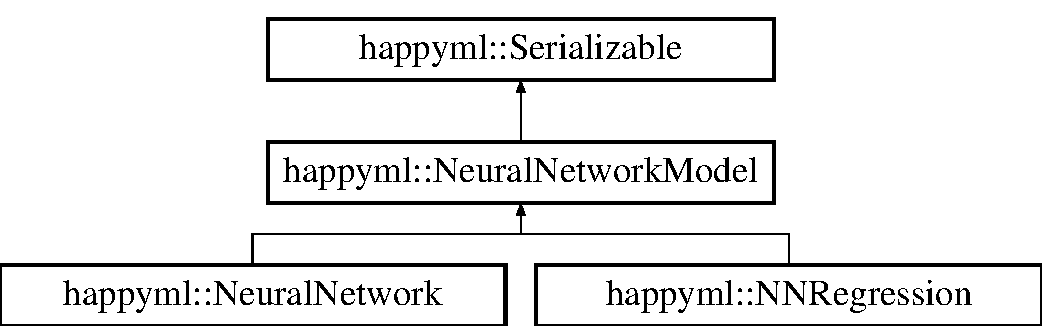
\includegraphics[height=3.000000cm]{classhappyml_1_1NeuralNetworkModel}
\end{center}
\end{figure}
\subsection*{Public Member Functions}
\begin{DoxyCompactItemize}
\item 
\hyperlink{classhappyml_1_1NeuralNetworkModel_a2ba8add6f01ebf3824967c43754ba96b}{Neural\+Network\+Model} (unsigned layers=0...)
\begin{DoxyCompactList}\small\item\em Creates a neural network with the layers and number of neurons indicated in the arguments. \end{DoxyCompactList}\item 
\hyperlink{classhappyml_1_1NeuralNetworkModel_a9db88c5a5fd88ab871f8237aab03b5ad}{Neural\+Network\+Model} (const vector$<$ unsigned $>$ \&layers)
\begin{DoxyCompactList}\small\item\em Creates a neural network with the layers and number of neurons indicated in the vector. \end{DoxyCompactList}\item 
\hyperlink{classhappyml_1_1NeuralNetworkModel_ad5359ce00a00346dab8433767f77988d}{Neural\+Network\+Model} (const vector$<$ mat $>$ \&w)
\begin{DoxyCompactList}\small\item\em Creates a neural network using the indicated weights matrices. \end{DoxyCompactList}\item 
\hyperlink{classhappyml_1_1NeuralNetworkModel_adadfa82c7b452789822dcb94ae5055d3}{Neural\+Network\+Model} (const \hyperlink{classhappyml_1_1NeuralNetworkModel}{Neural\+Network\+Model} \&nn)
\begin{DoxyCompactList}\small\item\em Creates a copy of a neural network. \end{DoxyCompactList}\item 
\hyperlink{classhappyml_1_1NeuralNetworkModel_a8ee4b9eae5590dc86f72e28c29fd1238}{$\sim$\+Neural\+Network\+Model} ()
\item 
vector$<$ mat $>$ \hyperlink{classhappyml_1_1NeuralNetworkModel_a9711fe856879e6e9db916ffd5479e136}{get\+Weights} () const 
\begin{DoxyCompactList}\small\item\em Returns a copy of all the weights of the neural network. \end{DoxyCompactList}\item 
unsigned \hyperlink{classhappyml_1_1NeuralNetworkModel_a3fd616a220f3e617359b96a31c27b921}{get\+Number\+Layers} () const 
\begin{DoxyCompactList}\small\item\em Returns the number of layers of the neural network counting the input and ouput layer. \end{DoxyCompactList}\item 
unsigned \hyperlink{classhappyml_1_1NeuralNetworkModel_a7bf0503214bcc6de9d3ad646ff7b1b92}{get\+Number\+Neurons} (unsigned layer) const 
\begin{DoxyCompactList}\small\item\em Returns the number of neurons on layer \textquotesingle{}layer\textquotesingle{}. \end{DoxyCompactList}\item 
void \hyperlink{classhappyml_1_1NeuralNetworkModel_a5591e0392dc1ec3d6d730ae355cc7f09}{read} (istream \&stream)
\begin{DoxyCompactList}\small\item\em Read the object from an input stream. \end{DoxyCompactList}\item 
void \hyperlink{classhappyml_1_1NeuralNetworkModel_acaae169ac128c0c707342960e7c048eb}{write} (ostream \&stream) const 
\begin{DoxyCompactList}\small\item\em Write the object to an output stream. \end{DoxyCompactList}\end{DoxyCompactItemize}
\subsection*{Protected Member Functions}
\begin{DoxyCompactItemize}
\item 
\hyperlink{classhappyml_1_1NeuralNetworkModel_a1fbb361d360e321f0b022a9016c0d067}{Neural\+Network\+Model} (unsigned layers, bool unused)
\begin{DoxyCompactList}\small\item\em Protected constructor that allow to create networks with the given number of layer but without neurons on each layer. \end{DoxyCompactList}\end{DoxyCompactItemize}
\subsection*{Protected Attributes}
\begin{DoxyCompactItemize}
\item 
unsigned \hyperlink{classhappyml_1_1NeuralNetworkModel_ac7e46ff5974de133f5863ee02b620096}{L}
\begin{DoxyCompactList}\small\item\em Number of layers -\/ 1. \end{DoxyCompactList}\item 
vector$<$ mat $>$ \hyperlink{classhappyml_1_1NeuralNetworkModel_a84c347de105f8a0fcf6907cee7e8200d}{weights}
\begin{DoxyCompactList}\small\item\em Weights of the neuronal network. \end{DoxyCompactList}\item 
vector$<$ unsigned $>$ \hyperlink{classhappyml_1_1NeuralNetworkModel_a36ee0888f3c3e0f3197bce8fbc57831d}{d}
\begin{DoxyCompactList}\small\item\em Number of neurons of each layer. \end{DoxyCompactList}\end{DoxyCompactItemize}


\subsection{Detailed Description}
Hypothesis that uses a network of neurons. 

The weights of each layer are represented using matrices.

This class contains a protected vector of matrices weights, a public getter and load/save methods. 

\subsection{Constructor \& Destructor Documentation}
\index{happyml\+::\+Neural\+Network\+Model@{happyml\+::\+Neural\+Network\+Model}!Neural\+Network\+Model@{Neural\+Network\+Model}}
\index{Neural\+Network\+Model@{Neural\+Network\+Model}!happyml\+::\+Neural\+Network\+Model@{happyml\+::\+Neural\+Network\+Model}}
\subsubsection[{\texorpdfstring{Neural\+Network\+Model(unsigned layers, bool unused)}{NeuralNetworkModel(unsigned layers, bool unused)}}]{\setlength{\rightskip}{0pt plus 5cm}happyml\+::\+Neural\+Network\+Model\+::\+Neural\+Network\+Model (
\begin{DoxyParamCaption}
\item[{unsigned}]{layers, }
\item[{bool}]{unused}
\end{DoxyParamCaption}
)\hspace{0.3cm}{\ttfamily [protected]}}\hypertarget{classhappyml_1_1NeuralNetworkModel_a1fbb361d360e321f0b022a9016c0d067}{}\label{classhappyml_1_1NeuralNetworkModel_a1fbb361d360e321f0b022a9016c0d067}


Protected constructor that allow to create networks with the given number of layer but without neurons on each layer. 

Used on subclases to enable variable args in constructors. The second parameter is unused and allows differentiate this constructor from the others. \index{happyml\+::\+Neural\+Network\+Model@{happyml\+::\+Neural\+Network\+Model}!Neural\+Network\+Model@{Neural\+Network\+Model}}
\index{Neural\+Network\+Model@{Neural\+Network\+Model}!happyml\+::\+Neural\+Network\+Model@{happyml\+::\+Neural\+Network\+Model}}
\subsubsection[{\texorpdfstring{Neural\+Network\+Model(unsigned layers=0...)}{NeuralNetworkModel(unsigned layers=0...)}}]{\setlength{\rightskip}{0pt plus 5cm}happyml\+::\+Neural\+Network\+Model\+::\+Neural\+Network\+Model (
\begin{DoxyParamCaption}
\item[{unsigned}]{layers = {\ttfamily 0...}}
\end{DoxyParamCaption}
)}\hypertarget{classhappyml_1_1NeuralNetworkModel_a2ba8add6f01ebf3824967c43754ba96b}{}\label{classhappyml_1_1NeuralNetworkModel_a2ba8add6f01ebf3824967c43754ba96b}


Creates a neural network with the layers and number of neurons indicated in the arguments. 

Initialize the weights to a random values.

By default (without parameters), creates an empty neural network without layers. Use load method to give values to the network.

With \hyperlink{classhappyml_1_1NeuralNetworkModel}{Neural\+Network\+Model} nn(2, 2, 1) a 2 layer network is created. In the input layer there are 2 neurons and 1 in the output. Using \hyperlink{classhappyml_1_1NeuralNetworkModel}{Neural\+Network\+Model} nn(3, 2, 4, 1) you add a hidden layer with 4 neurons.


\begin{DoxyParams}{Parameters}
{\em layers} & Number of layers, number of neurons on the input layer, number of neurons on the second layer... \\
\hline
\end{DoxyParams}
\index{happyml\+::\+Neural\+Network\+Model@{happyml\+::\+Neural\+Network\+Model}!Neural\+Network\+Model@{Neural\+Network\+Model}}
\index{Neural\+Network\+Model@{Neural\+Network\+Model}!happyml\+::\+Neural\+Network\+Model@{happyml\+::\+Neural\+Network\+Model}}
\subsubsection[{\texorpdfstring{Neural\+Network\+Model(const vector$<$ unsigned $>$ \&layers)}{NeuralNetworkModel(const vector< unsigned > &layers)}}]{\setlength{\rightskip}{0pt plus 5cm}happyml\+::\+Neural\+Network\+Model\+::\+Neural\+Network\+Model (
\begin{DoxyParamCaption}
\item[{const vector$<$ unsigned $>$ \&}]{layers}
\end{DoxyParamCaption}
)}\hypertarget{classhappyml_1_1NeuralNetworkModel_a9db88c5a5fd88ab871f8237aab03b5ad}{}\label{classhappyml_1_1NeuralNetworkModel_a9db88c5a5fd88ab871f8237aab03b5ad}


Creates a neural network with the layers and number of neurons indicated in the vector. 

Initialize the weights to a random values.


\begin{DoxyParams}{Parameters}
{\em layers} & Number of neurons on the input layer, number of neurons on the second layer... \\
\hline
\end{DoxyParams}
\index{happyml\+::\+Neural\+Network\+Model@{happyml\+::\+Neural\+Network\+Model}!Neural\+Network\+Model@{Neural\+Network\+Model}}
\index{Neural\+Network\+Model@{Neural\+Network\+Model}!happyml\+::\+Neural\+Network\+Model@{happyml\+::\+Neural\+Network\+Model}}
\subsubsection[{\texorpdfstring{Neural\+Network\+Model(const vector$<$ mat $>$ \&w)}{NeuralNetworkModel(const vector< mat > &w)}}]{\setlength{\rightskip}{0pt plus 5cm}happyml\+::\+Neural\+Network\+Model\+::\+Neural\+Network\+Model (
\begin{DoxyParamCaption}
\item[{const vector$<$ mat $>$ \&}]{w}
\end{DoxyParamCaption}
)}\hypertarget{classhappyml_1_1NeuralNetworkModel_ad5359ce00a00346dab8433767f77988d}{}\label{classhappyml_1_1NeuralNetworkModel_ad5359ce00a00346dab8433767f77988d}


Creates a neural network using the indicated weights matrices. 


\begin{DoxyParams}{Parameters}
{\em w} & Weights matrices to use. \\
\hline
\end{DoxyParams}
\index{happyml\+::\+Neural\+Network\+Model@{happyml\+::\+Neural\+Network\+Model}!Neural\+Network\+Model@{Neural\+Network\+Model}}
\index{Neural\+Network\+Model@{Neural\+Network\+Model}!happyml\+::\+Neural\+Network\+Model@{happyml\+::\+Neural\+Network\+Model}}
\subsubsection[{\texorpdfstring{Neural\+Network\+Model(const Neural\+Network\+Model \&nn)}{NeuralNetworkModel(const NeuralNetworkModel &nn)}}]{\setlength{\rightskip}{0pt plus 5cm}happyml\+::\+Neural\+Network\+Model\+::\+Neural\+Network\+Model (
\begin{DoxyParamCaption}
\item[{const {\bf Neural\+Network\+Model} \&}]{nn}
\end{DoxyParamCaption}
)}\hypertarget{classhappyml_1_1NeuralNetworkModel_adadfa82c7b452789822dcb94ae5055d3}{}\label{classhappyml_1_1NeuralNetworkModel_adadfa82c7b452789822dcb94ae5055d3}


Creates a copy of a neural network. 

\index{happyml\+::\+Neural\+Network\+Model@{happyml\+::\+Neural\+Network\+Model}!````~Neural\+Network\+Model@{$\sim$\+Neural\+Network\+Model}}
\index{````~Neural\+Network\+Model@{$\sim$\+Neural\+Network\+Model}!happyml\+::\+Neural\+Network\+Model@{happyml\+::\+Neural\+Network\+Model}}
\subsubsection[{\texorpdfstring{$\sim$\+Neural\+Network\+Model()}{~NeuralNetworkModel()}}]{\setlength{\rightskip}{0pt plus 5cm}happyml\+::\+Neural\+Network\+Model\+::$\sim$\+Neural\+Network\+Model (
\begin{DoxyParamCaption}
{}
\end{DoxyParamCaption}
)}\hypertarget{classhappyml_1_1NeuralNetworkModel_a8ee4b9eae5590dc86f72e28c29fd1238}{}\label{classhappyml_1_1NeuralNetworkModel_a8ee4b9eae5590dc86f72e28c29fd1238}


\subsection{Member Function Documentation}
\index{happyml\+::\+Neural\+Network\+Model@{happyml\+::\+Neural\+Network\+Model}!get\+Number\+Layers@{get\+Number\+Layers}}
\index{get\+Number\+Layers@{get\+Number\+Layers}!happyml\+::\+Neural\+Network\+Model@{happyml\+::\+Neural\+Network\+Model}}
\subsubsection[{\texorpdfstring{get\+Number\+Layers() const }{getNumberLayers() const }}]{\setlength{\rightskip}{0pt plus 5cm}unsigned happyml\+::\+Neural\+Network\+Model\+::get\+Number\+Layers (
\begin{DoxyParamCaption}
{}
\end{DoxyParamCaption}
) const\hspace{0.3cm}{\ttfamily [inline]}}\hypertarget{classhappyml_1_1NeuralNetworkModel_a3fd616a220f3e617359b96a31c27b921}{}\label{classhappyml_1_1NeuralNetworkModel_a3fd616a220f3e617359b96a31c27b921}


Returns the number of layers of the neural network counting the input and ouput layer. 

\begin{DoxyReturn}{Returns}
Number of layers of the network. 
\end{DoxyReturn}
\index{happyml\+::\+Neural\+Network\+Model@{happyml\+::\+Neural\+Network\+Model}!get\+Number\+Neurons@{get\+Number\+Neurons}}
\index{get\+Number\+Neurons@{get\+Number\+Neurons}!happyml\+::\+Neural\+Network\+Model@{happyml\+::\+Neural\+Network\+Model}}
\subsubsection[{\texorpdfstring{get\+Number\+Neurons(unsigned layer) const }{getNumberNeurons(unsigned layer) const }}]{\setlength{\rightskip}{0pt plus 5cm}unsigned happyml\+::\+Neural\+Network\+Model\+::get\+Number\+Neurons (
\begin{DoxyParamCaption}
\item[{unsigned}]{layer}
\end{DoxyParamCaption}
) const\hspace{0.3cm}{\ttfamily [inline]}}\hypertarget{classhappyml_1_1NeuralNetworkModel_a7bf0503214bcc6de9d3ad646ff7b1b92}{}\label{classhappyml_1_1NeuralNetworkModel_a7bf0503214bcc6de9d3ad646ff7b1b92}


Returns the number of neurons on layer \textquotesingle{}layer\textquotesingle{}. 

Layer number is not checked. Be sure that layer $<$ \hyperlink{classhappyml_1_1NeuralNetworkModel_a3fd616a220f3e617359b96a31c27b921}{get\+Number\+Layers()}.

\begin{DoxyReturn}{Returns}
Number of layers of the layer \textquotesingle{}layer\textquotesingle{}. 
\end{DoxyReturn}
\index{happyml\+::\+Neural\+Network\+Model@{happyml\+::\+Neural\+Network\+Model}!get\+Weights@{get\+Weights}}
\index{get\+Weights@{get\+Weights}!happyml\+::\+Neural\+Network\+Model@{happyml\+::\+Neural\+Network\+Model}}
\subsubsection[{\texorpdfstring{get\+Weights() const }{getWeights() const }}]{\setlength{\rightskip}{0pt plus 5cm}vector$<$mat$>$ happyml\+::\+Neural\+Network\+Model\+::get\+Weights (
\begin{DoxyParamCaption}
{}
\end{DoxyParamCaption}
) const\hspace{0.3cm}{\ttfamily [inline]}}\hypertarget{classhappyml_1_1NeuralNetworkModel_a9711fe856879e6e9db916ffd5479e136}{}\label{classhappyml_1_1NeuralNetworkModel_a9711fe856879e6e9db916ffd5479e136}


Returns a copy of all the weights of the neural network. 

\begin{DoxyReturn}{Returns}
Copy of all the weights of the neural network. 
\end{DoxyReturn}
\index{happyml\+::\+Neural\+Network\+Model@{happyml\+::\+Neural\+Network\+Model}!read@{read}}
\index{read@{read}!happyml\+::\+Neural\+Network\+Model@{happyml\+::\+Neural\+Network\+Model}}
\subsubsection[{\texorpdfstring{read(istream \&stream)}{read(istream &stream)}}]{\setlength{\rightskip}{0pt plus 5cm}void happyml\+::\+Neural\+Network\+Model\+::read (
\begin{DoxyParamCaption}
\item[{istream \&}]{stream}
\end{DoxyParamCaption}
)\hspace{0.3cm}{\ttfamily [virtual]}}\hypertarget{classhappyml_1_1NeuralNetworkModel_a5591e0392dc1ec3d6d730ae355cc7f09}{}\label{classhappyml_1_1NeuralNetworkModel_a5591e0392dc1ec3d6d730ae355cc7f09}


Read the object from an input stream. 


\begin{DoxyParams}{Parameters}
{\em stream} & Input stream. \\
\hline
\end{DoxyParams}


Implements \hyperlink{classhappyml_1_1Serializable_aef5c211d8e9c1c425b33c657824c2f0c}{happyml\+::\+Serializable}.

\index{happyml\+::\+Neural\+Network\+Model@{happyml\+::\+Neural\+Network\+Model}!write@{write}}
\index{write@{write}!happyml\+::\+Neural\+Network\+Model@{happyml\+::\+Neural\+Network\+Model}}
\subsubsection[{\texorpdfstring{write(ostream \&stream) const }{write(ostream &stream) const }}]{\setlength{\rightskip}{0pt plus 5cm}void happyml\+::\+Neural\+Network\+Model\+::write (
\begin{DoxyParamCaption}
\item[{ostream \&}]{stream}
\end{DoxyParamCaption}
) const\hspace{0.3cm}{\ttfamily [virtual]}}\hypertarget{classhappyml_1_1NeuralNetworkModel_acaae169ac128c0c707342960e7c048eb}{}\label{classhappyml_1_1NeuralNetworkModel_acaae169ac128c0c707342960e7c048eb}


Write the object to an output stream. 


\begin{DoxyParams}{Parameters}
{\em stream} & Output stream. \\
\hline
\end{DoxyParams}


Implements \hyperlink{classhappyml_1_1Serializable_a2d503e4c2e39c5be8a33bcc8b691949f}{happyml\+::\+Serializable}.



\subsection{Member Data Documentation}
\index{happyml\+::\+Neural\+Network\+Model@{happyml\+::\+Neural\+Network\+Model}!d@{d}}
\index{d@{d}!happyml\+::\+Neural\+Network\+Model@{happyml\+::\+Neural\+Network\+Model}}
\subsubsection[{\texorpdfstring{d}{d}}]{\setlength{\rightskip}{0pt plus 5cm}vector$<$unsigned$>$ happyml\+::\+Neural\+Network\+Model\+::d\hspace{0.3cm}{\ttfamily [protected]}}\hypertarget{classhappyml_1_1NeuralNetworkModel_a36ee0888f3c3e0f3197bce8fbc57831d}{}\label{classhappyml_1_1NeuralNetworkModel_a36ee0888f3c3e0f3197bce8fbc57831d}


Number of neurons of each layer. 

The size of this vector is $L + 1$.

d\mbox{[}0\mbox{]} -\/$>$ number of units of the input layer. d\mbox{[}L\mbox{]} -\/$>$ number of units of the output layer. \index{happyml\+::\+Neural\+Network\+Model@{happyml\+::\+Neural\+Network\+Model}!L@{L}}
\index{L@{L}!happyml\+::\+Neural\+Network\+Model@{happyml\+::\+Neural\+Network\+Model}}
\subsubsection[{\texorpdfstring{L}{L}}]{\setlength{\rightskip}{0pt plus 5cm}unsigned happyml\+::\+Neural\+Network\+Model\+::L\hspace{0.3cm}{\ttfamily [protected]}}\hypertarget{classhappyml_1_1NeuralNetworkModel_ac7e46ff5974de133f5863ee02b620096}{}\label{classhappyml_1_1NeuralNetworkModel_ac7e46ff5974de133f5863ee02b620096}


Number of layers -\/ 1. 

The input layer is the first layer (indexed as 0) and the output layer is the last one (indexed as L). \index{happyml\+::\+Neural\+Network\+Model@{happyml\+::\+Neural\+Network\+Model}!weights@{weights}}
\index{weights@{weights}!happyml\+::\+Neural\+Network\+Model@{happyml\+::\+Neural\+Network\+Model}}
\subsubsection[{\texorpdfstring{weights}{weights}}]{\setlength{\rightskip}{0pt plus 5cm}vector$<$mat$>$ happyml\+::\+Neural\+Network\+Model\+::weights\hspace{0.3cm}{\ttfamily [protected]}}\hypertarget{classhappyml_1_1NeuralNetworkModel_a84c347de105f8a0fcf6907cee7e8200d}{}\label{classhappyml_1_1NeuralNetworkModel_a84c347de105f8a0fcf6907cee7e8200d}


Weights of the neuronal network. 

The size of this vector is always $L$, but the first element is always a 0x0 matrix. 

The documentation for this class was generated from the following files\+:\begin{DoxyCompactItemize}
\item 
include/happyml/neural\+\_\+network/\hyperlink{neural__network__model_8h}{neural\+\_\+network\+\_\+model.\+h}\item 
src/neural\+\_\+network/\hyperlink{neural__network__model_8cpp}{neural\+\_\+network\+\_\+model.\+cpp}\end{DoxyCompactItemize}

\hypertarget{classhappyml_1_1NNRegression}{}\section{happyml\+:\+:N\+N\+Regression Class Reference}
\label{classhappyml_1_1NNRegression}\index{happyml\+::\+N\+N\+Regression@{happyml\+::\+N\+N\+Regression}}


{\ttfamily \#include $<$nn\+\_\+regression.\+h$>$}

Inheritance diagram for happyml\+:\+:N\+N\+Regression\+:\begin{figure}[H]
\begin{center}
\leavevmode
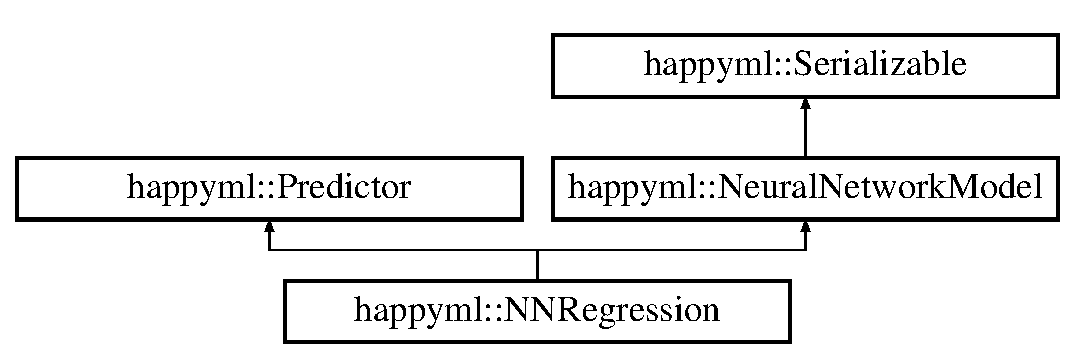
\includegraphics[height=3.000000cm]{classhappyml_1_1NNRegression}
\end{center}
\end{figure}
\subsection*{Public Member Functions}
\begin{DoxyCompactItemize}
\item 
\hyperlink{classhappyml_1_1NNRegression_a841009d2dd46074131720b68835bea93}{N\+N\+Regression} (unsigned layers...)
\item 
\hyperlink{classhappyml_1_1NNRegression_afc2740e5ec788112526934afe3ced3d0}{N\+N\+Regression} (const vector$<$ unsigned $>$ \&layers)
\item 
\hyperlink{classhappyml_1_1NNRegression_a02c9e45196687f410be7827bd637a577}{N\+N\+Regression} (const vector$<$ mat $>$ w)
\item 
\hyperlink{classhappyml_1_1NNRegression_a052de91d7e4224676d6240a389a52533}{N\+N\+Regression} (const \hyperlink{classhappyml_1_1NNRegression}{N\+N\+Regression} \&nn)
\item 
\hyperlink{classhappyml_1_1NNRegression_a05149a76d3e11653190b92bbef7a1f64}{$\sim$\+N\+N\+Regression} ()
\item 
double \hyperlink{classhappyml_1_1NNRegression_ac9c9dcd8d2cd4e9e6f1b742c5dd277b6}{train} (const \hyperlink{classhappyml_1_1DataSet}{Data\+Set} \&dataset, unsigned iter=500, float learning\+\_\+rate=0.\+1, float lambda=0)
\begin{DoxyCompactList}\small\item\em Train the neural network until the training loops over the data iter times. \end{DoxyCompactList}\item 
double \hyperlink{classhappyml_1_1NNRegression_aea4c134130125d22c3587b8a9d9c8e1b}{predict} (const \hyperlink{namespacehappyml_a03602d1ec49393790b8a0449f40cd01f}{Input} \&x) const 
\begin{DoxyCompactList}\small\item\em Uses the forward propagation algorithm to predict an output. \end{DoxyCompactList}\item 
vec \hyperlink{classhappyml_1_1NNRegression_af2aadc9111b4bd9cd89afb6847f1bb3f}{predict\+Vec} (const \hyperlink{namespacehappyml_a03602d1ec49393790b8a0449f40cd01f}{Input} \&x) const 
\item 
double \hyperlink{classhappyml_1_1NNRegression_a6f649a08fc94523a49e893ffad766896}{error} (const \hyperlink{classhappyml_1_1DataSet}{Data\+Set} \&) const 
\begin{DoxyCompactList}\small\item\em Compute the error of the predictor on the given dataset. \end{DoxyCompactList}\end{DoxyCompactItemize}
\subsection*{Additional Inherited Members}


\subsection{Constructor \& Destructor Documentation}
\index{happyml\+::\+N\+N\+Regression@{happyml\+::\+N\+N\+Regression}!N\+N\+Regression@{N\+N\+Regression}}
\index{N\+N\+Regression@{N\+N\+Regression}!happyml\+::\+N\+N\+Regression@{happyml\+::\+N\+N\+Regression}}
\subsubsection[{\texorpdfstring{N\+N\+Regression(unsigned layers...)}{NNRegression(unsigned layers...)}}]{\setlength{\rightskip}{0pt plus 5cm}happyml\+::\+N\+N\+Regression\+::\+N\+N\+Regression (
\begin{DoxyParamCaption}
\item[{unsigned}]{layers...}
\end{DoxyParamCaption}
)}\hypertarget{classhappyml_1_1NNRegression_a841009d2dd46074131720b68835bea93}{}\label{classhappyml_1_1NNRegression_a841009d2dd46074131720b68835bea93}
\index{happyml\+::\+N\+N\+Regression@{happyml\+::\+N\+N\+Regression}!N\+N\+Regression@{N\+N\+Regression}}
\index{N\+N\+Regression@{N\+N\+Regression}!happyml\+::\+N\+N\+Regression@{happyml\+::\+N\+N\+Regression}}
\subsubsection[{\texorpdfstring{N\+N\+Regression(const vector$<$ unsigned $>$ \&layers)}{NNRegression(const vector< unsigned > &layers)}}]{\setlength{\rightskip}{0pt plus 5cm}happyml\+::\+N\+N\+Regression\+::\+N\+N\+Regression (
\begin{DoxyParamCaption}
\item[{const vector$<$ unsigned $>$ \&}]{layers}
\end{DoxyParamCaption}
)\hspace{0.3cm}{\ttfamily [inline]}}\hypertarget{classhappyml_1_1NNRegression_afc2740e5ec788112526934afe3ced3d0}{}\label{classhappyml_1_1NNRegression_afc2740e5ec788112526934afe3ced3d0}
\index{happyml\+::\+N\+N\+Regression@{happyml\+::\+N\+N\+Regression}!N\+N\+Regression@{N\+N\+Regression}}
\index{N\+N\+Regression@{N\+N\+Regression}!happyml\+::\+N\+N\+Regression@{happyml\+::\+N\+N\+Regression}}
\subsubsection[{\texorpdfstring{N\+N\+Regression(const vector$<$ mat $>$ w)}{NNRegression(const vector< mat > w)}}]{\setlength{\rightskip}{0pt plus 5cm}happyml\+::\+N\+N\+Regression\+::\+N\+N\+Regression (
\begin{DoxyParamCaption}
\item[{const vector$<$ mat $>$}]{w}
\end{DoxyParamCaption}
)\hspace{0.3cm}{\ttfamily [inline]}}\hypertarget{classhappyml_1_1NNRegression_a02c9e45196687f410be7827bd637a577}{}\label{classhappyml_1_1NNRegression_a02c9e45196687f410be7827bd637a577}
\index{happyml\+::\+N\+N\+Regression@{happyml\+::\+N\+N\+Regression}!N\+N\+Regression@{N\+N\+Regression}}
\index{N\+N\+Regression@{N\+N\+Regression}!happyml\+::\+N\+N\+Regression@{happyml\+::\+N\+N\+Regression}}
\subsubsection[{\texorpdfstring{N\+N\+Regression(const N\+N\+Regression \&nn)}{NNRegression(const NNRegression &nn)}}]{\setlength{\rightskip}{0pt plus 5cm}happyml\+::\+N\+N\+Regression\+::\+N\+N\+Regression (
\begin{DoxyParamCaption}
\item[{const {\bf N\+N\+Regression} \&}]{nn}
\end{DoxyParamCaption}
)\hspace{0.3cm}{\ttfamily [inline]}}\hypertarget{classhappyml_1_1NNRegression_a052de91d7e4224676d6240a389a52533}{}\label{classhappyml_1_1NNRegression_a052de91d7e4224676d6240a389a52533}
\index{happyml\+::\+N\+N\+Regression@{happyml\+::\+N\+N\+Regression}!````~N\+N\+Regression@{$\sim$\+N\+N\+Regression}}
\index{````~N\+N\+Regression@{$\sim$\+N\+N\+Regression}!happyml\+::\+N\+N\+Regression@{happyml\+::\+N\+N\+Regression}}
\subsubsection[{\texorpdfstring{$\sim$\+N\+N\+Regression()}{~NNRegression()}}]{\setlength{\rightskip}{0pt plus 5cm}happyml\+::\+N\+N\+Regression\+::$\sim$\+N\+N\+Regression (
\begin{DoxyParamCaption}
{}
\end{DoxyParamCaption}
)\hspace{0.3cm}{\ttfamily [inline]}}\hypertarget{classhappyml_1_1NNRegression_a05149a76d3e11653190b92bbef7a1f64}{}\label{classhappyml_1_1NNRegression_a05149a76d3e11653190b92bbef7a1f64}


\subsection{Member Function Documentation}
\index{happyml\+::\+N\+N\+Regression@{happyml\+::\+N\+N\+Regression}!error@{error}}
\index{error@{error}!happyml\+::\+N\+N\+Regression@{happyml\+::\+N\+N\+Regression}}
\subsubsection[{\texorpdfstring{error(const Data\+Set \&) const }{error(const DataSet &) const }}]{\setlength{\rightskip}{0pt plus 5cm}double happyml\+::\+N\+N\+Regression\+::error (
\begin{DoxyParamCaption}
\item[{const {\bf Data\+Set} \&}]{dataset}
\end{DoxyParamCaption}
) const\hspace{0.3cm}{\ttfamily [virtual]}}\hypertarget{classhappyml_1_1NNRegression_a6f649a08fc94523a49e893ffad766896}{}\label{classhappyml_1_1NNRegression_a6f649a08fc94523a49e893ffad766896}


Compute the error of the predictor on the given dataset. 


\begin{DoxyParams}{Parameters}
{\em data} & Dataset with the correct output.\\
\hline
\end{DoxyParams}
\begin{DoxyReturn}{Returns}
Error of predicting the output of the given dataset. 
\end{DoxyReturn}


Reimplemented from \hyperlink{classhappyml_1_1Predictor_a59b022fac2ffa3a0254b75cb02b70dfe}{happyml\+::\+Predictor}.

\index{happyml\+::\+N\+N\+Regression@{happyml\+::\+N\+N\+Regression}!predict@{predict}}
\index{predict@{predict}!happyml\+::\+N\+N\+Regression@{happyml\+::\+N\+N\+Regression}}
\subsubsection[{\texorpdfstring{predict(const Input \&x) const }{predict(const Input &x) const }}]{\setlength{\rightskip}{0pt plus 5cm}double happyml\+::\+N\+N\+Regression\+::predict (
\begin{DoxyParamCaption}
\item[{const {\bf Input} \&}]{x}
\end{DoxyParamCaption}
) const\hspace{0.3cm}{\ttfamily [virtual]}}\hypertarget{classhappyml_1_1NNRegression_aea4c134130125d22c3587b8a9d9c8e1b}{}\label{classhappyml_1_1NNRegression_aea4c134130125d22c3587b8a9d9c8e1b}


Uses the forward propagation algorithm to predict an output. 


\begin{DoxyParams}{Parameters}
{\em x} & Input vector.\\
\hline
\end{DoxyParams}
\begin{DoxyReturn}{Returns}
Predicted value 
\end{DoxyReturn}


Implements \hyperlink{classhappyml_1_1Predictor_a07cf89d655e7642fd94c9b2a8fd0a04b}{happyml\+::\+Predictor}.

\index{happyml\+::\+N\+N\+Regression@{happyml\+::\+N\+N\+Regression}!predict\+Vec@{predict\+Vec}}
\index{predict\+Vec@{predict\+Vec}!happyml\+::\+N\+N\+Regression@{happyml\+::\+N\+N\+Regression}}
\subsubsection[{\texorpdfstring{predict\+Vec(const Input \&x) const }{predictVec(const Input &x) const }}]{\setlength{\rightskip}{0pt plus 5cm}vec happyml\+::\+N\+N\+Regression\+::predict\+Vec (
\begin{DoxyParamCaption}
\item[{const {\bf Input} \&}]{x}
\end{DoxyParamCaption}
) const}\hypertarget{classhappyml_1_1NNRegression_af2aadc9111b4bd9cd89afb6847f1bb3f}{}\label{classhappyml_1_1NNRegression_af2aadc9111b4bd9cd89afb6847f1bb3f}
\index{happyml\+::\+N\+N\+Regression@{happyml\+::\+N\+N\+Regression}!train@{train}}
\index{train@{train}!happyml\+::\+N\+N\+Regression@{happyml\+::\+N\+N\+Regression}}
\subsubsection[{\texorpdfstring{train(const Data\+Set \&dataset, unsigned iter=500, float learning\+\_\+rate=0.\+1, float lambda=0)}{train(const DataSet &dataset, unsigned iter=500, float learning_rate=0.1, float lambda=0)}}]{\setlength{\rightskip}{0pt plus 5cm}double happyml\+::\+N\+N\+Regression\+::train (
\begin{DoxyParamCaption}
\item[{const {\bf Data\+Set} \&}]{dataset, }
\item[{unsigned}]{iter = {\ttfamily 500}, }
\item[{float}]{learning\+\_\+rate = {\ttfamily 0.1}, }
\item[{float}]{lambda = {\ttfamily 0}}
\end{DoxyParamCaption}
)}\hypertarget{classhappyml_1_1NNRegression_ac9c9dcd8d2cd4e9e6f1b742c5dd277b6}{}\label{classhappyml_1_1NNRegression_ac9c9dcd8d2cd4e9e6f1b742c5dd277b6}


Train the neural network until the training loops over the data iter times. 


\begin{DoxyParams}{Parameters}
{\em dataset} & Training set $\mathcal{D}$. \\
\hline
{\em learning\+Rate} & Learning rate $\eta$. \\
\hline
{\em iter} & Number of iterations. \\
\hline
{\em lambda} & Regularization paramiter $\lambda$.\\
\hline
\end{DoxyParams}
\begin{DoxyReturn}{Returns}
Returns the error after the training. 
\end{DoxyReturn}


The documentation for this class was generated from the following files\+:\begin{DoxyCompactItemize}
\item 
include/happyml/neural\+\_\+network/\hyperlink{nn__regression_8h}{nn\+\_\+regression.\+h}\item 
src/neural\+\_\+network/\hyperlink{nn__regression_8cpp}{nn\+\_\+regression.\+cpp}\end{DoxyCompactItemize}

\hypertarget{classhappyml_1_1Normalizer}{}\section{happyml\+:\+:Normalizer Class Reference}
\label{classhappyml_1_1Normalizer}\index{happyml\+::\+Normalizer@{happyml\+::\+Normalizer}}


Normalizes a dataset using feature scaling\+: x\textquotesingle{} = x -\/ min(x) / (max(x) -\/ min(x))  




{\ttfamily \#include $<$normalizer.\+h$>$}

Inheritance diagram for happyml\+:\+:Normalizer\+:\begin{figure}[H]
\begin{center}
\leavevmode
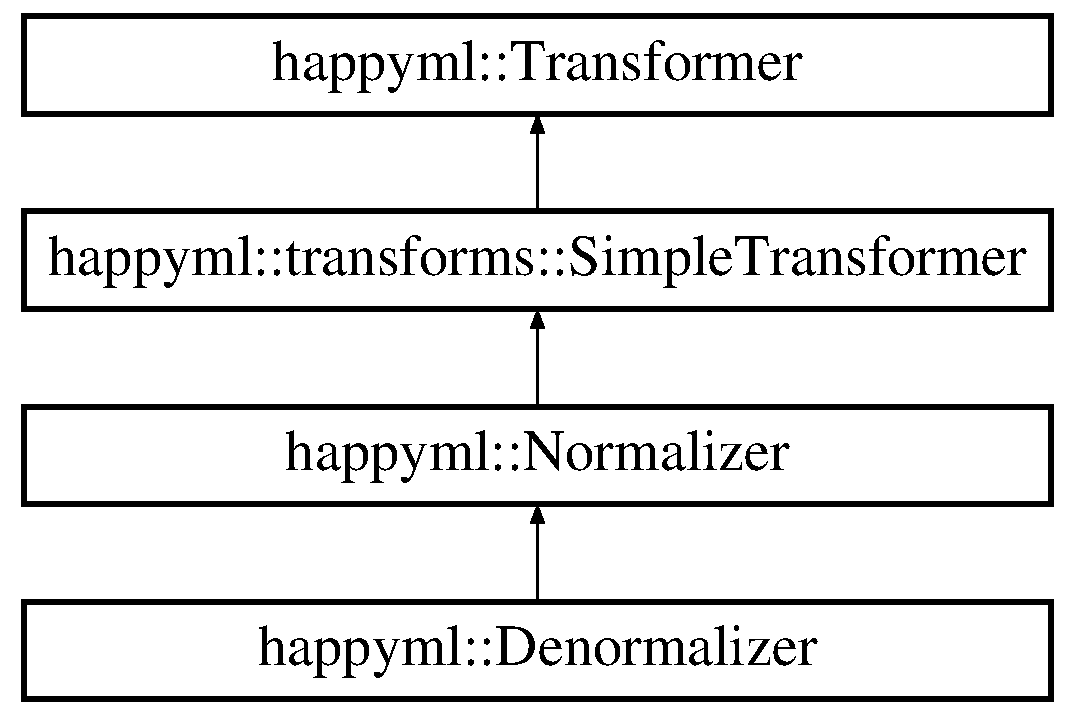
\includegraphics[height=4.000000cm]{classhappyml_1_1Normalizer}
\end{center}
\end{figure}
\subsection*{Public Member Functions}
\begin{DoxyCompactItemize}
\item 
\hyperlink{classhappyml_1_1Normalizer_af077d001899fed09a9abf17bf25e8024}{Normalizer} (const \hyperlink{classhappyml_1_1DataSet}{Data\+Set} \&dataset)
\begin{DoxyCompactList}\small\item\em Creates a normalizer that will use min and max data obtained from the dataset. \end{DoxyCompactList}\item 
\hyperlink{classhappyml_1_1Normalizer_a89b2ff31096640780e5232b73600b267}{Normalizer} (const mat \&x)
\begin{DoxyCompactList}\small\item\em Creates a normalizer that will use min and max data obtained from the matrix x. \end{DoxyCompactList}\item 
\hyperlink{classhappyml_1_1Normalizer_aa8a09a8e4f7ebe0cedc09fb5c2114841}{Normalizer} (const vec \&minvec, const vec \&maxvec)
\begin{DoxyCompactList}\small\item\em Creates a normalizer that will use the given min and max vectors. \end{DoxyCompactList}\item 
\hyperlink{classhappyml_1_1Normalizer_ac478c1302d6e3b66237af985e44265d2}{$\sim$\+Normalizer} ()
\item 
virtual void \hyperlink{classhappyml_1_1Normalizer_aeff0b4e117d69311cc5845c9915fa691}{apply} (mat \&x) const 
\end{DoxyCompactItemize}
\subsection*{Protected Member Functions}
\begin{DoxyCompactItemize}
\item 
void \hyperlink{classhappyml_1_1Normalizer_a7a11184002ab74861f61a6bad74482b5}{init} (const mat \&)
\end{DoxyCompactItemize}
\subsection*{Protected Attributes}
\begin{DoxyCompactItemize}
\item 
rowvec \hyperlink{classhappyml_1_1Normalizer_a0e7aece7fcdc71c49f6f4ecde5421a35}{minx}
\item 
rowvec \hyperlink{classhappyml_1_1Normalizer_abaafd2ccd9502013c4acc1254f1af75a}{maxx}
\item 
rowvec \hyperlink{classhappyml_1_1Normalizer_a3d6e869c3bbab4e960a219ff69c8a597}{rangex}
\item 
rowvec \hyperlink{classhappyml_1_1Normalizer_a793ede833b7279317f1ddca6ad8cbf66}{miny}
\item 
rowvec \hyperlink{classhappyml_1_1Normalizer_a3fdcdd3102e162de11b4ff833da8dc02}{maxy}
\end{DoxyCompactItemize}


\subsection{Detailed Description}
Normalizes a dataset using feature scaling\+: x\textquotesingle{} = x -\/ min(x) / (max(x) -\/ min(x)) 

\subsection{Constructor \& Destructor Documentation}
\index{happyml\+::\+Normalizer@{happyml\+::\+Normalizer}!Normalizer@{Normalizer}}
\index{Normalizer@{Normalizer}!happyml\+::\+Normalizer@{happyml\+::\+Normalizer}}
\subsubsection[{\texorpdfstring{Normalizer(const Data\+Set \&dataset)}{Normalizer(const DataSet &dataset)}}]{\setlength{\rightskip}{0pt plus 5cm}happyml\+::\+Normalizer\+::\+Normalizer (
\begin{DoxyParamCaption}
\item[{const {\bf Data\+Set} \&}]{dataset}
\end{DoxyParamCaption}
)\hspace{0.3cm}{\ttfamily [inline]}}\hypertarget{classhappyml_1_1Normalizer_af077d001899fed09a9abf17bf25e8024}{}\label{classhappyml_1_1Normalizer_af077d001899fed09a9abf17bf25e8024}


Creates a normalizer that will use min and max data obtained from the dataset. 


\begin{DoxyParams}{Parameters}
{\em dataset} & Dataset from which it will be extracted the min and max that will be use when apply normalization. \\
\hline
\end{DoxyParams}
\index{happyml\+::\+Normalizer@{happyml\+::\+Normalizer}!Normalizer@{Normalizer}}
\index{Normalizer@{Normalizer}!happyml\+::\+Normalizer@{happyml\+::\+Normalizer}}
\subsubsection[{\texorpdfstring{Normalizer(const mat \&x)}{Normalizer(const mat &x)}}]{\setlength{\rightskip}{0pt plus 5cm}happyml\+::\+Normalizer\+::\+Normalizer (
\begin{DoxyParamCaption}
\item[{const mat \&}]{x}
\end{DoxyParamCaption}
)\hspace{0.3cm}{\ttfamily [inline]}}\hypertarget{classhappyml_1_1Normalizer_a89b2ff31096640780e5232b73600b267}{}\label{classhappyml_1_1Normalizer_a89b2ff31096640780e5232b73600b267}


Creates a normalizer that will use min and max data obtained from the matrix x. 


\begin{DoxyParams}{Parameters}
{\em x} & Matrix from which it will be extracted the min and max that will be use when apply normalization. \\
\hline
\end{DoxyParams}
\index{happyml\+::\+Normalizer@{happyml\+::\+Normalizer}!Normalizer@{Normalizer}}
\index{Normalizer@{Normalizer}!happyml\+::\+Normalizer@{happyml\+::\+Normalizer}}
\subsubsection[{\texorpdfstring{Normalizer(const vec \&minvec, const vec \&maxvec)}{Normalizer(const vec &minvec, const vec &maxvec)}}]{\setlength{\rightskip}{0pt plus 5cm}happyml\+::\+Normalizer\+::\+Normalizer (
\begin{DoxyParamCaption}
\item[{const vec \&}]{minvec, }
\item[{const vec \&}]{maxvec}
\end{DoxyParamCaption}
)\hspace{0.3cm}{\ttfamily [inline]}}\hypertarget{classhappyml_1_1Normalizer_aa8a09a8e4f7ebe0cedc09fb5c2114841}{}\label{classhappyml_1_1Normalizer_aa8a09a8e4f7ebe0cedc09fb5c2114841}


Creates a normalizer that will use the given min and max vectors. 


\begin{DoxyParams}{Parameters}
{\em minvec} & Vector with the min numbers. \\
\hline
{\em maxvec} & Vector with the max numbers. \\
\hline
\end{DoxyParams}
\index{happyml\+::\+Normalizer@{happyml\+::\+Normalizer}!````~Normalizer@{$\sim$\+Normalizer}}
\index{````~Normalizer@{$\sim$\+Normalizer}!happyml\+::\+Normalizer@{happyml\+::\+Normalizer}}
\subsubsection[{\texorpdfstring{$\sim$\+Normalizer()}{~Normalizer()}}]{\setlength{\rightskip}{0pt plus 5cm}happyml\+::\+Normalizer\+::$\sim$\+Normalizer (
\begin{DoxyParamCaption}
{}
\end{DoxyParamCaption}
)\hspace{0.3cm}{\ttfamily [inline]}}\hypertarget{classhappyml_1_1Normalizer_ac478c1302d6e3b66237af985e44265d2}{}\label{classhappyml_1_1Normalizer_ac478c1302d6e3b66237af985e44265d2}


\subsection{Member Function Documentation}
\index{happyml\+::\+Normalizer@{happyml\+::\+Normalizer}!apply@{apply}}
\index{apply@{apply}!happyml\+::\+Normalizer@{happyml\+::\+Normalizer}}
\subsubsection[{\texorpdfstring{apply(mat \&x) const }{apply(mat &x) const }}]{\setlength{\rightskip}{0pt plus 5cm}void happyml\+::\+Normalizer\+::apply (
\begin{DoxyParamCaption}
\item[{mat \&}]{x}
\end{DoxyParamCaption}
) const\hspace{0.3cm}{\ttfamily [virtual]}}\hypertarget{classhappyml_1_1Normalizer_aeff0b4e117d69311cc5845c9915fa691}{}\label{classhappyml_1_1Normalizer_aeff0b4e117d69311cc5845c9915fa691}


Reimplemented from \hyperlink{classhappyml_1_1transforms_1_1SimpleTransformer_a2f38b1b4eb85dca83cb9f6ed9796da32}{happyml\+::transforms\+::\+Simple\+Transformer}.



Reimplemented in \hyperlink{classhappyml_1_1Denormalizer_a2f1aa35006d0573f07fc33e8f154c170}{happyml\+::\+Denormalizer}.

\index{happyml\+::\+Normalizer@{happyml\+::\+Normalizer}!init@{init}}
\index{init@{init}!happyml\+::\+Normalizer@{happyml\+::\+Normalizer}}
\subsubsection[{\texorpdfstring{init(const mat \&)}{init(const mat &)}}]{\setlength{\rightskip}{0pt plus 5cm}void happyml\+::\+Normalizer\+::init (
\begin{DoxyParamCaption}
\item[{const mat \&}]{x}
\end{DoxyParamCaption}
)\hspace{0.3cm}{\ttfamily [protected]}}\hypertarget{classhappyml_1_1Normalizer_a7a11184002ab74861f61a6bad74482b5}{}\label{classhappyml_1_1Normalizer_a7a11184002ab74861f61a6bad74482b5}


\subsection{Member Data Documentation}
\index{happyml\+::\+Normalizer@{happyml\+::\+Normalizer}!maxx@{maxx}}
\index{maxx@{maxx}!happyml\+::\+Normalizer@{happyml\+::\+Normalizer}}
\subsubsection[{\texorpdfstring{maxx}{maxx}}]{\setlength{\rightskip}{0pt plus 5cm}rowvec happyml\+::\+Normalizer\+::maxx\hspace{0.3cm}{\ttfamily [protected]}}\hypertarget{classhappyml_1_1Normalizer_abaafd2ccd9502013c4acc1254f1af75a}{}\label{classhappyml_1_1Normalizer_abaafd2ccd9502013c4acc1254f1af75a}
\index{happyml\+::\+Normalizer@{happyml\+::\+Normalizer}!maxy@{maxy}}
\index{maxy@{maxy}!happyml\+::\+Normalizer@{happyml\+::\+Normalizer}}
\subsubsection[{\texorpdfstring{maxy}{maxy}}]{\setlength{\rightskip}{0pt plus 5cm}rowvec happyml\+::\+Normalizer\+::maxy\hspace{0.3cm}{\ttfamily [protected]}}\hypertarget{classhappyml_1_1Normalizer_a3fdcdd3102e162de11b4ff833da8dc02}{}\label{classhappyml_1_1Normalizer_a3fdcdd3102e162de11b4ff833da8dc02}
\index{happyml\+::\+Normalizer@{happyml\+::\+Normalizer}!minx@{minx}}
\index{minx@{minx}!happyml\+::\+Normalizer@{happyml\+::\+Normalizer}}
\subsubsection[{\texorpdfstring{minx}{minx}}]{\setlength{\rightskip}{0pt plus 5cm}rowvec happyml\+::\+Normalizer\+::minx\hspace{0.3cm}{\ttfamily [protected]}}\hypertarget{classhappyml_1_1Normalizer_a0e7aece7fcdc71c49f6f4ecde5421a35}{}\label{classhappyml_1_1Normalizer_a0e7aece7fcdc71c49f6f4ecde5421a35}
\index{happyml\+::\+Normalizer@{happyml\+::\+Normalizer}!miny@{miny}}
\index{miny@{miny}!happyml\+::\+Normalizer@{happyml\+::\+Normalizer}}
\subsubsection[{\texorpdfstring{miny}{miny}}]{\setlength{\rightskip}{0pt plus 5cm}rowvec happyml\+::\+Normalizer\+::miny\hspace{0.3cm}{\ttfamily [protected]}}\hypertarget{classhappyml_1_1Normalizer_a793ede833b7279317f1ddca6ad8cbf66}{}\label{classhappyml_1_1Normalizer_a793ede833b7279317f1ddca6ad8cbf66}
\index{happyml\+::\+Normalizer@{happyml\+::\+Normalizer}!rangex@{rangex}}
\index{rangex@{rangex}!happyml\+::\+Normalizer@{happyml\+::\+Normalizer}}
\subsubsection[{\texorpdfstring{rangex}{rangex}}]{\setlength{\rightskip}{0pt plus 5cm}rowvec happyml\+::\+Normalizer\+::rangex\hspace{0.3cm}{\ttfamily [protected]}}\hypertarget{classhappyml_1_1Normalizer_a3d6e869c3bbab4e960a219ff69c8a597}{}\label{classhappyml_1_1Normalizer_a3d6e869c3bbab4e960a219ff69c8a597}


The documentation for this class was generated from the following files\+:\begin{DoxyCompactItemize}
\item 
include/happyml/transformers/\hyperlink{normalizer_8h}{normalizer.\+h}\item 
src/transformers/\hyperlink{normalizer_8cpp}{normalizer.\+cpp}\end{DoxyCompactItemize}

\hypertarget{classhappyml_1_1NormalizerXY}{}\section{happyml\+:\+:Normalizer\+XY Class Reference}
\label{classhappyml_1_1NormalizerXY}\index{happyml\+::\+Normalizer\+XY@{happyml\+::\+Normalizer\+XY}}


{\ttfamily \#include $<$normalizer.\+h$>$}

Inheritance diagram for happyml\+:\+:Normalizer\+XY\+:\begin{figure}[H]
\begin{center}
\leavevmode
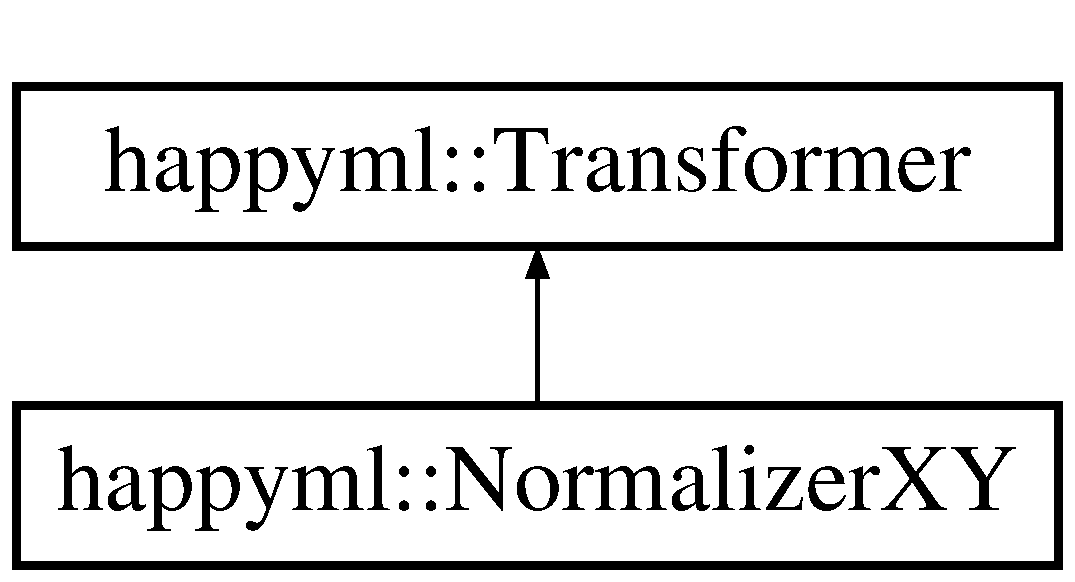
\includegraphics[height=2.000000cm]{classhappyml_1_1NormalizerXY}
\end{center}
\end{figure}
\subsection*{Public Member Functions}
\begin{DoxyCompactItemize}
\item 
\hyperlink{classhappyml_1_1NormalizerXY_a6d6a78fc840a6a0c6eed005c4491de86}{Normalizer\+XY} (const \hyperlink{classhappyml_1_1DataSet}{Data\+Set} \&d)
\item 
\hyperlink{classhappyml_1_1NormalizerXY_aa565dd9fcfa196e0f6dfdc6084cb4c14}{Normalizer\+XY} (const \hyperlink{classhappyml_1_1Normalizer}{Normalizer} \&x, const \hyperlink{classhappyml_1_1Normalizer}{Normalizer} \&y)
\item 
\hyperlink{classhappyml_1_1Normalizer}{Normalizer} \hyperlink{classhappyml_1_1NormalizerXY_afd0208937e983073f1e1c919bca368d3}{get\+NormalizerX} () const 
\item 
\hyperlink{classhappyml_1_1Normalizer}{Normalizer} \hyperlink{classhappyml_1_1NormalizerXY_a29f7f1cf3c2fda6fc21cbf5e976ec7e7}{get\+NormalizerY} () const 
\item 
void \hyperlink{classhappyml_1_1NormalizerXY_ac843088ef9e2189ed719f4556ba111e2}{apply} (\hyperlink{classhappyml_1_1DataSet}{Data\+Set} \&d) const 
\begin{DoxyCompactList}\small\item\em Applies all the transformations at the given dataset. \end{DoxyCompactList}\item 
\hyperlink{namespacehappyml_a03602d1ec49393790b8a0449f40cd01f}{Input} \hyperlink{classhappyml_1_1NormalizerXY_a0f10be1b98dfc3125990310ee649ee8e}{apply} (const \hyperlink{namespacehappyml_a03602d1ec49393790b8a0449f40cd01f}{Input} \&input) const 
\begin{DoxyCompactList}\small\item\em Applies all the transformations at the given input. \end{DoxyCompactList}\item 
vec \hyperlink{classhappyml_1_1NormalizerXY_ad09b59cf6e131a52412b98670854c62a}{apply\+Output} (const vec \&output) const 
\end{DoxyCompactItemize}
\subsection*{Protected Attributes}
\begin{DoxyCompactItemize}
\item 
\hyperlink{classhappyml_1_1Normalizer}{Normalizer} \hyperlink{classhappyml_1_1NormalizerXY_aedf3f87518e5e04fc2ec66aaa99e358a}{nx}
\item 
\hyperlink{classhappyml_1_1Normalizer}{Normalizer} \hyperlink{classhappyml_1_1NormalizerXY_a0f544e4bc2461e124cae233125c2a52e}{ny}
\end{DoxyCompactItemize}
\subsection*{Friends}
\begin{DoxyCompactItemize}
\item 
class \hyperlink{classhappyml_1_1NormalizerXY_a1360ec07e064939d46865e7132cbec87}{Denormalizer\+XY}
\end{DoxyCompactItemize}


\subsection{Constructor \& Destructor Documentation}
\index{happyml\+::\+Normalizer\+XY@{happyml\+::\+Normalizer\+XY}!Normalizer\+XY@{Normalizer\+XY}}
\index{Normalizer\+XY@{Normalizer\+XY}!happyml\+::\+Normalizer\+XY@{happyml\+::\+Normalizer\+XY}}
\subsubsection[{\texorpdfstring{Normalizer\+X\+Y(const Data\+Set \&d)}{NormalizerXY(const DataSet &d)}}]{\setlength{\rightskip}{0pt plus 5cm}happyml\+::\+Normalizer\+X\+Y\+::\+Normalizer\+XY (
\begin{DoxyParamCaption}
\item[{const {\bf Data\+Set} \&}]{d}
\end{DoxyParamCaption}
)\hspace{0.3cm}{\ttfamily [inline]}}\hypertarget{classhappyml_1_1NormalizerXY_a6d6a78fc840a6a0c6eed005c4491de86}{}\label{classhappyml_1_1NormalizerXY_a6d6a78fc840a6a0c6eed005c4491de86}
\index{happyml\+::\+Normalizer\+XY@{happyml\+::\+Normalizer\+XY}!Normalizer\+XY@{Normalizer\+XY}}
\index{Normalizer\+XY@{Normalizer\+XY}!happyml\+::\+Normalizer\+XY@{happyml\+::\+Normalizer\+XY}}
\subsubsection[{\texorpdfstring{Normalizer\+X\+Y(const Normalizer \&x, const Normalizer \&y)}{NormalizerXY(const Normalizer &x, const Normalizer &y)}}]{\setlength{\rightskip}{0pt plus 5cm}happyml\+::\+Normalizer\+X\+Y\+::\+Normalizer\+XY (
\begin{DoxyParamCaption}
\item[{const {\bf Normalizer} \&}]{x, }
\item[{const {\bf Normalizer} \&}]{y}
\end{DoxyParamCaption}
)\hspace{0.3cm}{\ttfamily [inline]}}\hypertarget{classhappyml_1_1NormalizerXY_aa565dd9fcfa196e0f6dfdc6084cb4c14}{}\label{classhappyml_1_1NormalizerXY_aa565dd9fcfa196e0f6dfdc6084cb4c14}


\subsection{Member Function Documentation}
\index{happyml\+::\+Normalizer\+XY@{happyml\+::\+Normalizer\+XY}!apply@{apply}}
\index{apply@{apply}!happyml\+::\+Normalizer\+XY@{happyml\+::\+Normalizer\+XY}}
\subsubsection[{\texorpdfstring{apply(\+Data\+Set \&d) const }{apply(DataSet &d) const }}]{\setlength{\rightskip}{0pt plus 5cm}void happyml\+::\+Normalizer\+X\+Y\+::apply (
\begin{DoxyParamCaption}
\item[{{\bf Data\+Set} \&}]{dataset}
\end{DoxyParamCaption}
) const\hspace{0.3cm}{\ttfamily [inline]}, {\ttfamily [virtual]}}\hypertarget{classhappyml_1_1NormalizerXY_ac843088ef9e2189ed719f4556ba111e2}{}\label{classhappyml_1_1NormalizerXY_ac843088ef9e2189ed719f4556ba111e2}


Applies all the transformations at the given dataset. 


\begin{DoxyParams}{Parameters}
{\em dataset} & Dataset to transform. \\
\hline
\end{DoxyParams}


Reimplemented from \hyperlink{classhappyml_1_1Transformer_a169a2a8434124c1dd8e671bca2cfa71d}{happyml\+::\+Transformer}.

\index{happyml\+::\+Normalizer\+XY@{happyml\+::\+Normalizer\+XY}!apply@{apply}}
\index{apply@{apply}!happyml\+::\+Normalizer\+XY@{happyml\+::\+Normalizer\+XY}}
\subsubsection[{\texorpdfstring{apply(const Input \&input) const }{apply(const Input &input) const }}]{\setlength{\rightskip}{0pt plus 5cm}{\bf Input} happyml\+::\+Normalizer\+X\+Y\+::apply (
\begin{DoxyParamCaption}
\item[{const {\bf Input} \&}]{input}
\end{DoxyParamCaption}
) const\hspace{0.3cm}{\ttfamily [inline]}, {\ttfamily [virtual]}}\hypertarget{classhappyml_1_1NormalizerXY_a0f10be1b98dfc3125990310ee649ee8e}{}\label{classhappyml_1_1NormalizerXY_a0f10be1b98dfc3125990310ee649ee8e}


Applies all the transformations at the given input. 


\begin{DoxyParams}{Parameters}
{\em input} & Input to transform.\\
\hline
\end{DoxyParams}
\begin{DoxyReturn}{Returns}
A transformated version of the input. 
\end{DoxyReturn}


Reimplemented from \hyperlink{classhappyml_1_1Transformer_a3e0eb67990c90c461466307fdefab45c}{happyml\+::\+Transformer}.

\index{happyml\+::\+Normalizer\+XY@{happyml\+::\+Normalizer\+XY}!apply\+Output@{apply\+Output}}
\index{apply\+Output@{apply\+Output}!happyml\+::\+Normalizer\+XY@{happyml\+::\+Normalizer\+XY}}
\subsubsection[{\texorpdfstring{apply\+Output(const vec \&output) const }{applyOutput(const vec &output) const }}]{\setlength{\rightskip}{0pt plus 5cm}vec happyml\+::\+Normalizer\+X\+Y\+::apply\+Output (
\begin{DoxyParamCaption}
\item[{const vec \&}]{output}
\end{DoxyParamCaption}
) const\hspace{0.3cm}{\ttfamily [inline]}}\hypertarget{classhappyml_1_1NormalizerXY_ad09b59cf6e131a52412b98670854c62a}{}\label{classhappyml_1_1NormalizerXY_ad09b59cf6e131a52412b98670854c62a}
\index{happyml\+::\+Normalizer\+XY@{happyml\+::\+Normalizer\+XY}!get\+NormalizerX@{get\+NormalizerX}}
\index{get\+NormalizerX@{get\+NormalizerX}!happyml\+::\+Normalizer\+XY@{happyml\+::\+Normalizer\+XY}}
\subsubsection[{\texorpdfstring{get\+Normalizer\+X() const }{getNormalizerX() const }}]{\setlength{\rightskip}{0pt plus 5cm}{\bf Normalizer} happyml\+::\+Normalizer\+X\+Y\+::get\+NormalizerX (
\begin{DoxyParamCaption}
{}
\end{DoxyParamCaption}
) const\hspace{0.3cm}{\ttfamily [inline]}}\hypertarget{classhappyml_1_1NormalizerXY_afd0208937e983073f1e1c919bca368d3}{}\label{classhappyml_1_1NormalizerXY_afd0208937e983073f1e1c919bca368d3}
\index{happyml\+::\+Normalizer\+XY@{happyml\+::\+Normalizer\+XY}!get\+NormalizerY@{get\+NormalizerY}}
\index{get\+NormalizerY@{get\+NormalizerY}!happyml\+::\+Normalizer\+XY@{happyml\+::\+Normalizer\+XY}}
\subsubsection[{\texorpdfstring{get\+Normalizer\+Y() const }{getNormalizerY() const }}]{\setlength{\rightskip}{0pt plus 5cm}{\bf Normalizer} happyml\+::\+Normalizer\+X\+Y\+::get\+NormalizerY (
\begin{DoxyParamCaption}
{}
\end{DoxyParamCaption}
) const\hspace{0.3cm}{\ttfamily [inline]}}\hypertarget{classhappyml_1_1NormalizerXY_a29f7f1cf3c2fda6fc21cbf5e976ec7e7}{}\label{classhappyml_1_1NormalizerXY_a29f7f1cf3c2fda6fc21cbf5e976ec7e7}


\subsection{Friends And Related Function Documentation}
\index{happyml\+::\+Normalizer\+XY@{happyml\+::\+Normalizer\+XY}!Denormalizer\+XY@{Denormalizer\+XY}}
\index{Denormalizer\+XY@{Denormalizer\+XY}!happyml\+::\+Normalizer\+XY@{happyml\+::\+Normalizer\+XY}}
\subsubsection[{\texorpdfstring{Denormalizer\+XY}{DenormalizerXY}}]{\setlength{\rightskip}{0pt plus 5cm}friend class {\bf Denormalizer\+XY}\hspace{0.3cm}{\ttfamily [friend]}}\hypertarget{classhappyml_1_1NormalizerXY_a1360ec07e064939d46865e7132cbec87}{}\label{classhappyml_1_1NormalizerXY_a1360ec07e064939d46865e7132cbec87}


\subsection{Member Data Documentation}
\index{happyml\+::\+Normalizer\+XY@{happyml\+::\+Normalizer\+XY}!nx@{nx}}
\index{nx@{nx}!happyml\+::\+Normalizer\+XY@{happyml\+::\+Normalizer\+XY}}
\subsubsection[{\texorpdfstring{nx}{nx}}]{\setlength{\rightskip}{0pt plus 5cm}{\bf Normalizer} happyml\+::\+Normalizer\+X\+Y\+::nx\hspace{0.3cm}{\ttfamily [protected]}}\hypertarget{classhappyml_1_1NormalizerXY_aedf3f87518e5e04fc2ec66aaa99e358a}{}\label{classhappyml_1_1NormalizerXY_aedf3f87518e5e04fc2ec66aaa99e358a}
\index{happyml\+::\+Normalizer\+XY@{happyml\+::\+Normalizer\+XY}!ny@{ny}}
\index{ny@{ny}!happyml\+::\+Normalizer\+XY@{happyml\+::\+Normalizer\+XY}}
\subsubsection[{\texorpdfstring{ny}{ny}}]{\setlength{\rightskip}{0pt plus 5cm}{\bf Normalizer} happyml\+::\+Normalizer\+X\+Y\+::ny\hspace{0.3cm}{\ttfamily [protected]}}\hypertarget{classhappyml_1_1NormalizerXY_a0f544e4bc2461e124cae233125c2a52e}{}\label{classhappyml_1_1NormalizerXY_a0f544e4bc2461e124cae233125c2a52e}


The documentation for this class was generated from the following file\+:\begin{DoxyCompactItemize}
\item 
include/happyml/transformers/\hyperlink{normalizer_8h}{normalizer.\+h}\end{DoxyCompactItemize}

\hypertarget{classhappyml_1_1PCA}{}\section{happyml\+:\+:P\+CA Class Reference}
\label{classhappyml_1_1PCA}\index{happyml\+::\+P\+CA@{happyml\+::\+P\+CA}}


Dimensionality reduction using \hyperlink{classhappyml_1_1PCA}{P\+CA}.  




{\ttfamily \#include $<$pca.\+h$>$}

Inheritance diagram for happyml\+:\+:P\+CA\+:\begin{figure}[H]
\begin{center}
\leavevmode
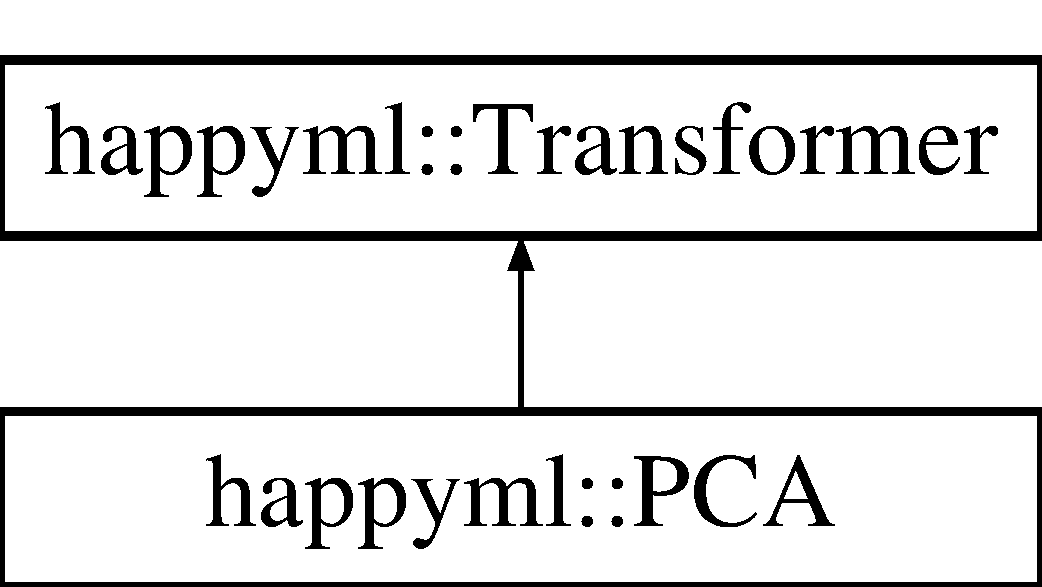
\includegraphics[height=2.000000cm]{classhappyml_1_1PCA}
\end{center}
\end{figure}
\subsection*{Public Member Functions}
\begin{DoxyCompactItemize}
\item 
\hyperlink{classhappyml_1_1PCA_a20ccc8033fb2addfe1607f12137e8c7a}{P\+CA} (const \hyperlink{classhappyml_1_1DataSet}{Data\+Set} \&dataset, double n)
\begin{DoxyCompactList}\small\item\em Creates a \hyperlink{classhappyml_1_1PCA}{P\+CA} extractor using the dataset data. \end{DoxyCompactList}\item 
\hyperlink{classhappyml_1_1PCA_aa03c90a06460ad6d76b7516454d709ec}{P\+CA} (const mat \&x, double n)
\begin{DoxyCompactList}\small\item\em Creates a \hyperlink{classhappyml_1_1PCA}{P\+CA} extractor using the matrix data. \end{DoxyCompactList}\item 
\hyperlink{classhappyml_1_1PCA_a10d3820f23ccde93ef029846ae1dd418}{$\sim$\+P\+CA} ()
\item 
double \hyperlink{classhappyml_1_1PCA_afec8e7b4f8bb8cbe6bd460fb278017a6}{get\+Retained\+Variance} () const 
\begin{DoxyCompactList}\small\item\em Returns the retained data variance of the \hyperlink{classhappyml_1_1PCA}{P\+CA} transformation. \end{DoxyCompactList}\item 
void \hyperlink{classhappyml_1_1PCA_a298495b3f3cf0ed3b623392a6f89b719}{apply} (\hyperlink{classhappyml_1_1DataSet}{Data\+Set} \&dataset) const 
\begin{DoxyCompactList}\small\item\em Applies all the transformations at the given dataset. \end{DoxyCompactList}\item 
void \hyperlink{classhappyml_1_1PCA_a3ac3cbbf12595272526b126ba2107d8e}{apply} (mat \&x) const 
\item 
\hyperlink{namespacehappyml_a03602d1ec49393790b8a0449f40cd01f}{Input} \hyperlink{classhappyml_1_1PCA_a2a630892c653832287bb3df4ab002d51}{apply} (const \hyperlink{namespacehappyml_a03602d1ec49393790b8a0449f40cd01f}{Input} \&input) const 
\begin{DoxyCompactList}\small\item\em Applies all the transformations at the given input. \end{DoxyCompactList}\end{DoxyCompactItemize}
\subsection*{Protected Attributes}
\begin{DoxyCompactItemize}
\item 
rowvec \hyperlink{classhappyml_1_1PCA_af7086a802a48818da96b850c6627114f}{mean\+Vec}
\item 
vec \hyperlink{classhappyml_1_1PCA_a0cb529e7070933c17b407a28a182a1fa}{eig\+Val}
\item 
mat \hyperlink{classhappyml_1_1PCA_aaaf28f625e92e1985beee5bba9fa2a56}{eig\+Vec}
\item 
mat \hyperlink{classhappyml_1_1PCA_a59819d057d5adab4a5ff3619ed73e80b}{cov\+Mat}
\item 
int \hyperlink{classhappyml_1_1PCA_a5f2ee80482a6e93d6591e9d674c2b197}{k}
\item 
double \hyperlink{classhappyml_1_1PCA_a1e7148cef7385f41f04010a827ec0899}{min\+Var}
\end{DoxyCompactItemize}


\subsection{Detailed Description}
Dimensionality reduction using \hyperlink{classhappyml_1_1PCA}{P\+CA}. 

\subsection{Constructor \& Destructor Documentation}
\index{happyml\+::\+P\+CA@{happyml\+::\+P\+CA}!P\+CA@{P\+CA}}
\index{P\+CA@{P\+CA}!happyml\+::\+P\+CA@{happyml\+::\+P\+CA}}
\subsubsection[{\texorpdfstring{P\+C\+A(const Data\+Set \&dataset, double n)}{PCA(const DataSet &dataset, double n)}}]{\setlength{\rightskip}{0pt plus 5cm}happyml\+::\+P\+C\+A\+::\+P\+CA (
\begin{DoxyParamCaption}
\item[{const {\bf Data\+Set} \&}]{dataset, }
\item[{double}]{n}
\end{DoxyParamCaption}
)}\hypertarget{classhappyml_1_1PCA_a20ccc8033fb2addfe1607f12137e8c7a}{}\label{classhappyml_1_1PCA_a20ccc8033fb2addfe1607f12137e8c7a}


Creates a \hyperlink{classhappyml_1_1PCA}{P\+CA} extractor using the dataset data. 


\begin{DoxyParams}{Parameters}
{\em dataset} & Dataset from which the eigenvecs for the \hyperlink{classhappyml_1_1PCA}{P\+CA} will be extracted. \\
\hline
{\em n} & Number of dimension to preserve or min mariance if it is a number between 0 and 1. \\
\hline
\end{DoxyParams}
\index{happyml\+::\+P\+CA@{happyml\+::\+P\+CA}!P\+CA@{P\+CA}}
\index{P\+CA@{P\+CA}!happyml\+::\+P\+CA@{happyml\+::\+P\+CA}}
\subsubsection[{\texorpdfstring{P\+C\+A(const mat \&x, double n)}{PCA(const mat &x, double n)}}]{\setlength{\rightskip}{0pt plus 5cm}happyml\+::\+P\+C\+A\+::\+P\+CA (
\begin{DoxyParamCaption}
\item[{const mat \&}]{x, }
\item[{double}]{n}
\end{DoxyParamCaption}
)}\hypertarget{classhappyml_1_1PCA_aa03c90a06460ad6d76b7516454d709ec}{}\label{classhappyml_1_1PCA_aa03c90a06460ad6d76b7516454d709ec}


Creates a \hyperlink{classhappyml_1_1PCA}{P\+CA} extractor using the matrix data. 


\begin{DoxyParams}{Parameters}
{\em x} & Matrix from which the eigenvecs for the \hyperlink{classhappyml_1_1PCA}{P\+CA} will be extracted. \\
\hline
{\em n} & Number of dimension to preserve or min mariance if it is a number between 0 and 1. \\
\hline
\end{DoxyParams}
\index{happyml\+::\+P\+CA@{happyml\+::\+P\+CA}!````~P\+CA@{$\sim$\+P\+CA}}
\index{````~P\+CA@{$\sim$\+P\+CA}!happyml\+::\+P\+CA@{happyml\+::\+P\+CA}}
\subsubsection[{\texorpdfstring{$\sim$\+P\+C\+A()}{~PCA()}}]{\setlength{\rightskip}{0pt plus 5cm}happyml\+::\+P\+C\+A\+::$\sim$\+P\+CA (
\begin{DoxyParamCaption}
{}
\end{DoxyParamCaption}
)\hspace{0.3cm}{\ttfamily [inline]}}\hypertarget{classhappyml_1_1PCA_a10d3820f23ccde93ef029846ae1dd418}{}\label{classhappyml_1_1PCA_a10d3820f23ccde93ef029846ae1dd418}


\subsection{Member Function Documentation}
\index{happyml\+::\+P\+CA@{happyml\+::\+P\+CA}!apply@{apply}}
\index{apply@{apply}!happyml\+::\+P\+CA@{happyml\+::\+P\+CA}}
\subsubsection[{\texorpdfstring{apply(\+Data\+Set \&dataset) const }{apply(DataSet &dataset) const }}]{\setlength{\rightskip}{0pt plus 5cm}void happyml\+::\+P\+C\+A\+::apply (
\begin{DoxyParamCaption}
\item[{{\bf Data\+Set} \&}]{dataset}
\end{DoxyParamCaption}
) const\hspace{0.3cm}{\ttfamily [virtual]}}\hypertarget{classhappyml_1_1PCA_a298495b3f3cf0ed3b623392a6f89b719}{}\label{classhappyml_1_1PCA_a298495b3f3cf0ed3b623392a6f89b719}


Applies all the transformations at the given dataset. 


\begin{DoxyParams}{Parameters}
{\em dataset} & Dataset to transform. \\
\hline
\end{DoxyParams}


Reimplemented from \hyperlink{classhappyml_1_1Transformer_a169a2a8434124c1dd8e671bca2cfa71d}{happyml\+::\+Transformer}.

\index{happyml\+::\+P\+CA@{happyml\+::\+P\+CA}!apply@{apply}}
\index{apply@{apply}!happyml\+::\+P\+CA@{happyml\+::\+P\+CA}}
\subsubsection[{\texorpdfstring{apply(mat \&x) const }{apply(mat &x) const }}]{\setlength{\rightskip}{0pt plus 5cm}void happyml\+::\+P\+C\+A\+::apply (
\begin{DoxyParamCaption}
\item[{mat \&}]{x}
\end{DoxyParamCaption}
) const}\hypertarget{classhappyml_1_1PCA_a3ac3cbbf12595272526b126ba2107d8e}{}\label{classhappyml_1_1PCA_a3ac3cbbf12595272526b126ba2107d8e}
\index{happyml\+::\+P\+CA@{happyml\+::\+P\+CA}!apply@{apply}}
\index{apply@{apply}!happyml\+::\+P\+CA@{happyml\+::\+P\+CA}}
\subsubsection[{\texorpdfstring{apply(const Input \&input) const }{apply(const Input &input) const }}]{\setlength{\rightskip}{0pt plus 5cm}{\bf Input} happyml\+::\+P\+C\+A\+::apply (
\begin{DoxyParamCaption}
\item[{const {\bf Input} \&}]{input}
\end{DoxyParamCaption}
) const\hspace{0.3cm}{\ttfamily [virtual]}}\hypertarget{classhappyml_1_1PCA_a2a630892c653832287bb3df4ab002d51}{}\label{classhappyml_1_1PCA_a2a630892c653832287bb3df4ab002d51}


Applies all the transformations at the given input. 


\begin{DoxyParams}{Parameters}
{\em input} & Input to transform.\\
\hline
\end{DoxyParams}
\begin{DoxyReturn}{Returns}
A transformated version of the input. 
\end{DoxyReturn}


Reimplemented from \hyperlink{classhappyml_1_1Transformer_a3e0eb67990c90c461466307fdefab45c}{happyml\+::\+Transformer}.

\index{happyml\+::\+P\+CA@{happyml\+::\+P\+CA}!get\+Retained\+Variance@{get\+Retained\+Variance}}
\index{get\+Retained\+Variance@{get\+Retained\+Variance}!happyml\+::\+P\+CA@{happyml\+::\+P\+CA}}
\subsubsection[{\texorpdfstring{get\+Retained\+Variance() const }{getRetainedVariance() const }}]{\setlength{\rightskip}{0pt plus 5cm}double happyml\+::\+P\+C\+A\+::get\+Retained\+Variance (
\begin{DoxyParamCaption}
{}
\end{DoxyParamCaption}
) const\hspace{0.3cm}{\ttfamily [inline]}}\hypertarget{classhappyml_1_1PCA_afec8e7b4f8bb8cbe6bd460fb278017a6}{}\label{classhappyml_1_1PCA_afec8e7b4f8bb8cbe6bd460fb278017a6}


Returns the retained data variance of the \hyperlink{classhappyml_1_1PCA}{P\+CA} transformation. 

It\textquotesingle{}s a number between 0 and 1. If you pass a min variance to the constructor remember that the retained variance is $>$= the min variance choosen.

\begin{DoxyReturn}{Returns}
The retained data variance of the \hyperlink{classhappyml_1_1PCA}{P\+CA} transformation. 
\end{DoxyReturn}


\subsection{Member Data Documentation}
\index{happyml\+::\+P\+CA@{happyml\+::\+P\+CA}!cov\+Mat@{cov\+Mat}}
\index{cov\+Mat@{cov\+Mat}!happyml\+::\+P\+CA@{happyml\+::\+P\+CA}}
\subsubsection[{\texorpdfstring{cov\+Mat}{covMat}}]{\setlength{\rightskip}{0pt plus 5cm}mat happyml\+::\+P\+C\+A\+::cov\+Mat\hspace{0.3cm}{\ttfamily [protected]}}\hypertarget{classhappyml_1_1PCA_a59819d057d5adab4a5ff3619ed73e80b}{}\label{classhappyml_1_1PCA_a59819d057d5adab4a5ff3619ed73e80b}
\index{happyml\+::\+P\+CA@{happyml\+::\+P\+CA}!eig\+Val@{eig\+Val}}
\index{eig\+Val@{eig\+Val}!happyml\+::\+P\+CA@{happyml\+::\+P\+CA}}
\subsubsection[{\texorpdfstring{eig\+Val}{eigVal}}]{\setlength{\rightskip}{0pt plus 5cm}vec happyml\+::\+P\+C\+A\+::eig\+Val\hspace{0.3cm}{\ttfamily [protected]}}\hypertarget{classhappyml_1_1PCA_a0cb529e7070933c17b407a28a182a1fa}{}\label{classhappyml_1_1PCA_a0cb529e7070933c17b407a28a182a1fa}
\index{happyml\+::\+P\+CA@{happyml\+::\+P\+CA}!eig\+Vec@{eig\+Vec}}
\index{eig\+Vec@{eig\+Vec}!happyml\+::\+P\+CA@{happyml\+::\+P\+CA}}
\subsubsection[{\texorpdfstring{eig\+Vec}{eigVec}}]{\setlength{\rightskip}{0pt plus 5cm}mat happyml\+::\+P\+C\+A\+::eig\+Vec\hspace{0.3cm}{\ttfamily [protected]}}\hypertarget{classhappyml_1_1PCA_aaaf28f625e92e1985beee5bba9fa2a56}{}\label{classhappyml_1_1PCA_aaaf28f625e92e1985beee5bba9fa2a56}
\index{happyml\+::\+P\+CA@{happyml\+::\+P\+CA}!k@{k}}
\index{k@{k}!happyml\+::\+P\+CA@{happyml\+::\+P\+CA}}
\subsubsection[{\texorpdfstring{k}{k}}]{\setlength{\rightskip}{0pt plus 5cm}int happyml\+::\+P\+C\+A\+::k\hspace{0.3cm}{\ttfamily [protected]}}\hypertarget{classhappyml_1_1PCA_a5f2ee80482a6e93d6591e9d674c2b197}{}\label{classhappyml_1_1PCA_a5f2ee80482a6e93d6591e9d674c2b197}
\index{happyml\+::\+P\+CA@{happyml\+::\+P\+CA}!mean\+Vec@{mean\+Vec}}
\index{mean\+Vec@{mean\+Vec}!happyml\+::\+P\+CA@{happyml\+::\+P\+CA}}
\subsubsection[{\texorpdfstring{mean\+Vec}{meanVec}}]{\setlength{\rightskip}{0pt plus 5cm}rowvec happyml\+::\+P\+C\+A\+::mean\+Vec\hspace{0.3cm}{\ttfamily [protected]}}\hypertarget{classhappyml_1_1PCA_af7086a802a48818da96b850c6627114f}{}\label{classhappyml_1_1PCA_af7086a802a48818da96b850c6627114f}
\index{happyml\+::\+P\+CA@{happyml\+::\+P\+CA}!min\+Var@{min\+Var}}
\index{min\+Var@{min\+Var}!happyml\+::\+P\+CA@{happyml\+::\+P\+CA}}
\subsubsection[{\texorpdfstring{min\+Var}{minVar}}]{\setlength{\rightskip}{0pt plus 5cm}double happyml\+::\+P\+C\+A\+::min\+Var\hspace{0.3cm}{\ttfamily [protected]}}\hypertarget{classhappyml_1_1PCA_a1e7148cef7385f41f04010a827ec0899}{}\label{classhappyml_1_1PCA_a1e7148cef7385f41f04010a827ec0899}


The documentation for this class was generated from the following files\+:\begin{DoxyCompactItemize}
\item 
include/happyml/transformers/\hyperlink{pca_8h}{pca.\+h}\item 
src/transformers/\hyperlink{pca_8cpp}{pca.\+cpp}\end{DoxyCompactItemize}

\hypertarget{classhappyml_1_1Perceptron}{}\section{happyml\+:\+:Perceptron Class Reference}
\label{classhappyml_1_1Perceptron}\index{happyml\+::\+Perceptron@{happyml\+::\+Perceptron}}


{\ttfamily \#include $<$perceptron.\+h$>$}

Inheritance diagram for happyml\+:\+:Perceptron\+:\begin{figure}[H]
\begin{center}
\leavevmode
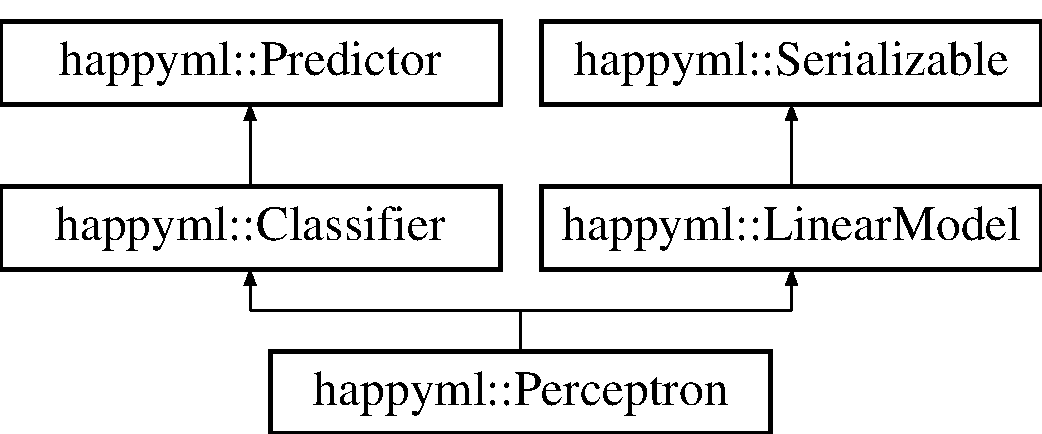
\includegraphics[height=3.000000cm]{classhappyml_1_1Perceptron}
\end{center}
\end{figure}
\subsection*{Public Member Functions}
\begin{DoxyCompactItemize}
\item 
\hyperlink{classhappyml_1_1Perceptron_afda225f54fc7810f431310380ad67934}{Perceptron} (unsigned d=0)
\begin{DoxyCompactList}\small\item\em Creates a perceptron with the indicated input size. \end{DoxyCompactList}\item 
\hyperlink{classhappyml_1_1Perceptron_a087a141d78442d353165ba8de91061a0}{Perceptron} (const vec \&weights)
\begin{DoxyCompactList}\small\item\em Creates a perceptron with the indicated weights. \end{DoxyCompactList}\item 
\hyperlink{classhappyml_1_1Perceptron_a15bca77ab91b58708d6d7506fbf5af96}{Perceptron} (const \hyperlink{classhappyml_1_1LinearModel}{Linear\+Model} \&lm)
\item 
double \hyperlink{classhappyml_1_1Perceptron_aa5b2a16fa72ef8575c8d4778b993fedd}{train} (const \hyperlink{classhappyml_1_1DataSet}{Data\+Set} \&data, unsigned iter)
\begin{DoxyCompactList}\small\item\em Train the perceptron until the training loops over the data n\+Times, or classifies all correctly. \end{DoxyCompactList}\item 
double \hyperlink{classhappyml_1_1Perceptron_aaa3c4d2a5235d6b5498de77f926c15f3}{predict} (const \hyperlink{namespacehappyml_a03602d1ec49393790b8a0449f40cd01f}{Input} \&x) const 
\begin{DoxyCompactList}\small\item\em Classifies an input vector. \end{DoxyCompactList}\item 
double \hyperlink{classhappyml_1_1Perceptron_aff79f084e1f9261e4e10feda0a5e74dd}{error} (const \hyperlink{classhappyml_1_1DataSet}{Data\+Set} \&data) const 
\begin{DoxyCompactList}\small\item\em Compute the error of the perceptron on the given dataset. \end{DoxyCompactList}\end{DoxyCompactItemize}
\subsection*{Additional Inherited Members}


\subsection{Constructor \& Destructor Documentation}
\index{happyml\+::\+Perceptron@{happyml\+::\+Perceptron}!Perceptron@{Perceptron}}
\index{Perceptron@{Perceptron}!happyml\+::\+Perceptron@{happyml\+::\+Perceptron}}
\subsubsection[{\texorpdfstring{Perceptron(unsigned d=0)}{Perceptron(unsigned d=0)}}]{\setlength{\rightskip}{0pt plus 5cm}happyml\+::\+Perceptron\+::\+Perceptron (
\begin{DoxyParamCaption}
\item[{unsigned}]{d = {\ttfamily 0}}
\end{DoxyParamCaption}
)\hspace{0.3cm}{\ttfamily [inline]}}\hypertarget{classhappyml_1_1Perceptron_afda225f54fc7810f431310380ad67934}{}\label{classhappyml_1_1Perceptron_afda225f54fc7810f431310380ad67934}


Creates a perceptron with the indicated input size. 


\begin{DoxyParams}{Parameters}
{\em d} & Dimension $d$ of the input feature vectors. \\
\hline
\end{DoxyParams}
\index{happyml\+::\+Perceptron@{happyml\+::\+Perceptron}!Perceptron@{Perceptron}}
\index{Perceptron@{Perceptron}!happyml\+::\+Perceptron@{happyml\+::\+Perceptron}}
\subsubsection[{\texorpdfstring{Perceptron(const vec \&weights)}{Perceptron(const vec &weights)}}]{\setlength{\rightskip}{0pt plus 5cm}happyml\+::\+Perceptron\+::\+Perceptron (
\begin{DoxyParamCaption}
\item[{const vec \&}]{weights}
\end{DoxyParamCaption}
)\hspace{0.3cm}{\ttfamily [inline]}}\hypertarget{classhappyml_1_1Perceptron_a087a141d78442d353165ba8de91061a0}{}\label{classhappyml_1_1Perceptron_a087a141d78442d353165ba8de91061a0}


Creates a perceptron with the indicated weights. 


\begin{DoxyParams}{Parameters}
{\em weights} & Weight vector with $d + 1$ dimensions. \\
\hline
\end{DoxyParams}
\index{happyml\+::\+Perceptron@{happyml\+::\+Perceptron}!Perceptron@{Perceptron}}
\index{Perceptron@{Perceptron}!happyml\+::\+Perceptron@{happyml\+::\+Perceptron}}
\subsubsection[{\texorpdfstring{Perceptron(const Linear\+Model \&lm)}{Perceptron(const LinearModel &lm)}}]{\setlength{\rightskip}{0pt plus 5cm}happyml\+::\+Perceptron\+::\+Perceptron (
\begin{DoxyParamCaption}
\item[{const {\bf Linear\+Model} \&}]{lm}
\end{DoxyParamCaption}
)\hspace{0.3cm}{\ttfamily [inline]}}\hypertarget{classhappyml_1_1Perceptron_a15bca77ab91b58708d6d7506fbf5af96}{}\label{classhappyml_1_1Perceptron_a15bca77ab91b58708d6d7506fbf5af96}


\subsection{Member Function Documentation}
\index{happyml\+::\+Perceptron@{happyml\+::\+Perceptron}!error@{error}}
\index{error@{error}!happyml\+::\+Perceptron@{happyml\+::\+Perceptron}}
\subsubsection[{\texorpdfstring{error(const Data\+Set \&data) const }{error(const DataSet &data) const }}]{\setlength{\rightskip}{0pt plus 5cm}double happyml\+::\+Perceptron\+::error (
\begin{DoxyParamCaption}
\item[{const {\bf Data\+Set} \&}]{data}
\end{DoxyParamCaption}
) const\hspace{0.3cm}{\ttfamily [virtual]}}\hypertarget{classhappyml_1_1Perceptron_aff79f084e1f9261e4e10feda0a5e74dd}{}\label{classhappyml_1_1Perceptron_aff79f084e1f9261e4e10feda0a5e74dd}


Compute the error of the perceptron on the given dataset. 


\begin{DoxyParams}{Parameters}
{\em data} & Dataset with the correct output.\\
\hline
\end{DoxyParams}
\begin{DoxyReturn}{Returns}
Error of classify the given dataset. It\textquotesingle{}s in the interval $[0, 1]$. 
\end{DoxyReturn}


Reimplemented from \hyperlink{classhappyml_1_1Predictor_a59b022fac2ffa3a0254b75cb02b70dfe}{happyml\+::\+Predictor}.

\index{happyml\+::\+Perceptron@{happyml\+::\+Perceptron}!predict@{predict}}
\index{predict@{predict}!happyml\+::\+Perceptron@{happyml\+::\+Perceptron}}
\subsubsection[{\texorpdfstring{predict(const Input \&x) const }{predict(const Input &x) const }}]{\setlength{\rightskip}{0pt plus 5cm}double happyml\+::\+Perceptron\+::predict (
\begin{DoxyParamCaption}
\item[{const {\bf Input} \&}]{x}
\end{DoxyParamCaption}
) const\hspace{0.3cm}{\ttfamily [virtual]}}\hypertarget{classhappyml_1_1Perceptron_aaa3c4d2a5235d6b5498de77f926c15f3}{}\label{classhappyml_1_1Perceptron_aaa3c4d2a5235d6b5498de77f926c15f3}


Classifies an input vector. 

\begin{DoxyReturn}{Returns}
$-1$ or $+1$. 
\end{DoxyReturn}


Implements \hyperlink{classhappyml_1_1Predictor_a07cf89d655e7642fd94c9b2a8fd0a04b}{happyml\+::\+Predictor}.

\index{happyml\+::\+Perceptron@{happyml\+::\+Perceptron}!train@{train}}
\index{train@{train}!happyml\+::\+Perceptron@{happyml\+::\+Perceptron}}
\subsubsection[{\texorpdfstring{train(const Data\+Set \&data, unsigned iter)}{train(const DataSet &data, unsigned iter)}}]{\setlength{\rightskip}{0pt plus 5cm}double happyml\+::\+Perceptron\+::train (
\begin{DoxyParamCaption}
\item[{const {\bf Data\+Set} \&}]{data, }
\item[{unsigned}]{iter}
\end{DoxyParamCaption}
)}\hypertarget{classhappyml_1_1Perceptron_aa5b2a16fa72ef8575c8d4778b993fedd}{}\label{classhappyml_1_1Perceptron_aa5b2a16fa72ef8575c8d4778b993fedd}


Train the perceptron until the training loops over the data n\+Times, or classifies all correctly. 

Data must contain the $x_0 = 1$ property.


\begin{DoxyParams}{Parameters}
{\em data} & Training set. \\
\hline
{\em iter} & Maximun number of iterations.\\
\hline
\end{DoxyParams}
\begin{DoxyReturn}{Returns}
Returns the error of the best perceptron found. 
\end{DoxyReturn}


The documentation for this class was generated from the following files\+:\begin{DoxyCompactItemize}
\item 
include/happyml/perceptron/\hyperlink{perceptron_8h}{perceptron.\+h}\item 
src/perceptron/\hyperlink{perceptron_8cpp}{perceptron.\+cpp}\end{DoxyCompactItemize}

\hypertarget{classhappyml_1_1transforms_1_1Pow}{}\section{happyml\+:\+:transforms\+:\+:Pow Class Reference}
\label{classhappyml_1_1transforms_1_1Pow}\index{happyml\+::transforms\+::\+Pow@{happyml\+::transforms\+::\+Pow}}


{\ttfamily \#include $<$transformer.\+h$>$}

Inheritance diagram for happyml\+:\+:transforms\+:\+:Pow\+:\begin{figure}[H]
\begin{center}
\leavevmode
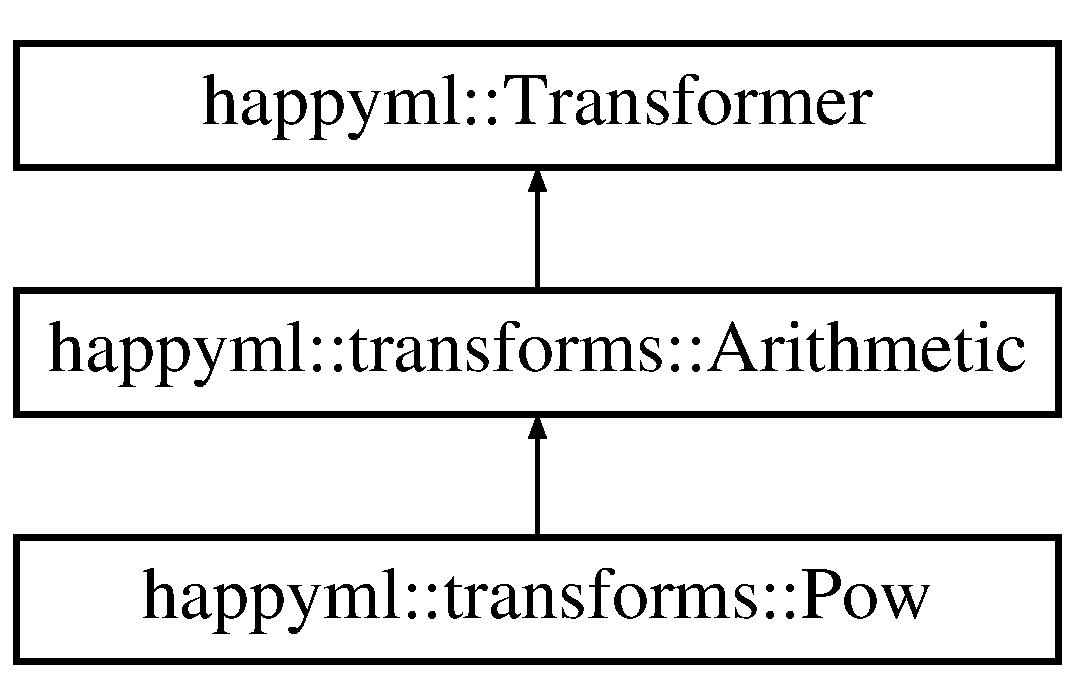
\includegraphics[height=3.000000cm]{classhappyml_1_1transforms_1_1Pow}
\end{center}
\end{figure}
\subsection*{Public Member Functions}
\begin{DoxyCompactItemize}
\item 
\hyperlink{classhappyml_1_1transforms_1_1Pow_a8a62bc6a54d71315313753dc71dfc9e5}{Pow} (int f, double p, bool nf=false)
\item 
void \hyperlink{classhappyml_1_1transforms_1_1Pow_af6d691fc3afbff2ee8f85db1725c2ea8}{apply} (mat \&x, int col) const 
\end{DoxyCompactItemize}
\subsection*{Additional Inherited Members}


\subsection{Constructor \& Destructor Documentation}
\index{happyml\+::transforms\+::\+Pow@{happyml\+::transforms\+::\+Pow}!Pow@{Pow}}
\index{Pow@{Pow}!happyml\+::transforms\+::\+Pow@{happyml\+::transforms\+::\+Pow}}
\subsubsection[{\texorpdfstring{Pow(int f, double p, bool nf=false)}{Pow(int f, double p, bool nf=false)}}]{\setlength{\rightskip}{0pt plus 5cm}happyml\+::transforms\+::\+Pow\+::\+Pow (
\begin{DoxyParamCaption}
\item[{int}]{f, }
\item[{double}]{p, }
\item[{bool}]{nf = {\ttfamily false}}
\end{DoxyParamCaption}
)\hspace{0.3cm}{\ttfamily [inline]}}\hypertarget{classhappyml_1_1transforms_1_1Pow_a8a62bc6a54d71315313753dc71dfc9e5}{}\label{classhappyml_1_1transforms_1_1Pow_a8a62bc6a54d71315313753dc71dfc9e5}


\subsection{Member Function Documentation}
\index{happyml\+::transforms\+::\+Pow@{happyml\+::transforms\+::\+Pow}!apply@{apply}}
\index{apply@{apply}!happyml\+::transforms\+::\+Pow@{happyml\+::transforms\+::\+Pow}}
\subsubsection[{\texorpdfstring{apply(mat \&x, int col) const }{apply(mat &x, int col) const }}]{\setlength{\rightskip}{0pt plus 5cm}void happyml\+::transforms\+::\+Pow\+::apply (
\begin{DoxyParamCaption}
\item[{mat \&}]{x, }
\item[{int}]{col}
\end{DoxyParamCaption}
) const\hspace{0.3cm}{\ttfamily [virtual]}}\hypertarget{classhappyml_1_1transforms_1_1Pow_af6d691fc3afbff2ee8f85db1725c2ea8}{}\label{classhappyml_1_1transforms_1_1Pow_af6d691fc3afbff2ee8f85db1725c2ea8}


Implements \hyperlink{classhappyml_1_1transforms_1_1Arithmetic_a85191dcd8734e18424b92b870d7b9d73}{happyml\+::transforms\+::\+Arithmetic}.



The documentation for this class was generated from the following files\+:\begin{DoxyCompactItemize}
\item 
include/happyml/transformers/\hyperlink{transformer_8h}{transformer.\+h}\item 
src/transformers/\hyperlink{transformer_8cpp}{transformer.\+cpp}\end{DoxyCompactItemize}

\hypertarget{classhappyml_1_1Predictor}{}\section{happyml\+:\+:Predictor Class Reference}
\label{classhappyml_1_1Predictor}\index{happyml\+::\+Predictor@{happyml\+::\+Predictor}}


Abstract class that represent an algorithm that predict an output or classifies an input vector.  




{\ttfamily \#include $<$predictor.\+h$>$}

Inheritance diagram for happyml\+:\+:Predictor\+:\begin{figure}[H]
\begin{center}
\leavevmode
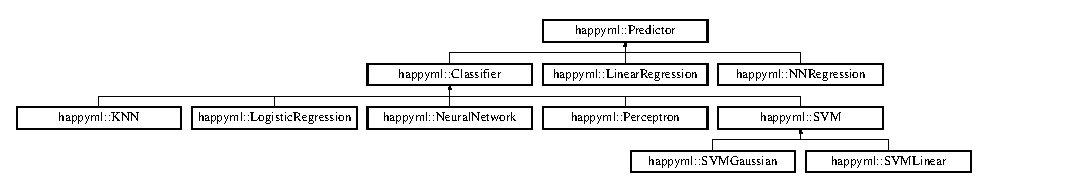
\includegraphics[height=2.085661cm]{classhappyml_1_1Predictor}
\end{center}
\end{figure}
\subsection*{Public Member Functions}
\begin{DoxyCompactItemize}
\item 
virtual double \hyperlink{classhappyml_1_1Predictor_a07cf89d655e7642fd94c9b2a8fd0a04b}{predict} (const \hyperlink{namespacehappyml_a03602d1ec49393790b8a0449f40cd01f}{Input} \&x) const  =0
\begin{DoxyCompactList}\small\item\em Predict an output from an input vector. \end{DoxyCompactList}\item 
virtual double \hyperlink{classhappyml_1_1Predictor_aeb20c07843cf4a2b7df76b2f0d0e0b13}{error} (const \hyperlink{namespacehappyml_a03602d1ec49393790b8a0449f40cd01f}{Input} \&x, double y) const 
\begin{DoxyCompactList}\small\item\em Compute the error of the predictor in a given input. \end{DoxyCompactList}\item 
virtual double \hyperlink{classhappyml_1_1Predictor_a59b022fac2ffa3a0254b75cb02b70dfe}{error} (const \hyperlink{classhappyml_1_1DataSet}{Data\+Set} \&dataset) const 
\begin{DoxyCompactList}\small\item\em Compute the error of the predictor on the given dataset. \end{DoxyCompactList}\item 
virtual void \hyperlink{classhappyml_1_1Predictor_a57e1704162af45ff6501a49c2cd3dada}{save\+Sampling} (const string \&filename, double minx\+\_\+1, double maxx\+\_\+1, unsigned samples\+\_\+1, double minx\+\_\+2, double maxx\+\_\+2, unsigned samples\+\_\+2, const \hyperlink{classhappyml_1_1Transformer}{Transformer} \&t=\hyperlink{classhappyml_1_1Transformer}{Transformer}()) const 
\begin{DoxyCompactList}\small\item\em Saves the value of predicting the output of the predicter on the rectangular area defined between $(minx_1, minx_2)$ and $(maxx_1, maxx_2)$ points. \end{DoxyCompactList}\item 
virtual void \hyperlink{classhappyml_1_1Predictor_a7be2a09809a15f9eef51ca37c4632cb7}{save\+Sampling} (const string \&filename, double minx, double maxx, unsigned samples, const \hyperlink{classhappyml_1_1Transformer}{Transformer} \&t=\hyperlink{classhappyml_1_1Transformer}{Transformer}()) const 
\begin{DoxyCompactList}\small\item\em Saves the value of predicting the output of the predicter in the segment $[minx, maxx]$. \end{DoxyCompactList}\end{DoxyCompactItemize}


\subsection{Detailed Description}
Abstract class that represent an algorithm that predict an output or classifies an input vector. 

\subsection{Member Function Documentation}
\index{happyml\+::\+Predictor@{happyml\+::\+Predictor}!error@{error}}
\index{error@{error}!happyml\+::\+Predictor@{happyml\+::\+Predictor}}
\subsubsection[{\texorpdfstring{error(const Input \&x, double y) const }{error(const Input &x, double y) const }}]{\setlength{\rightskip}{0pt plus 5cm}double happyml\+::\+Predictor\+::error (
\begin{DoxyParamCaption}
\item[{const {\bf Input} \&}]{x, }
\item[{double}]{y}
\end{DoxyParamCaption}
) const\hspace{0.3cm}{\ttfamily [virtual]}}\hypertarget{classhappyml_1_1Predictor_aeb20c07843cf4a2b7df76b2f0d0e0b13}{}\label{classhappyml_1_1Predictor_aeb20c07843cf4a2b7df76b2f0d0e0b13}


Compute the error of the predictor in a given input. 

By default it computes the square diff.


\begin{DoxyParams}{Parameters}
{\em x} & The input vector. \\
\hline
{\em y} & Correct output.\\
\hline
\end{DoxyParams}
\begin{DoxyReturn}{Returns}
Error of the predicted value comparate to y. 
\end{DoxyReturn}


Reimplemented in \hyperlink{classhappyml_1_1Classifier_ac72f1b0b689aaff5078978ae198318df}{happyml\+::\+Classifier}.

\index{happyml\+::\+Predictor@{happyml\+::\+Predictor}!error@{error}}
\index{error@{error}!happyml\+::\+Predictor@{happyml\+::\+Predictor}}
\subsubsection[{\texorpdfstring{error(const Data\+Set \&dataset) const }{error(const DataSet &dataset) const }}]{\setlength{\rightskip}{0pt plus 5cm}double happyml\+::\+Predictor\+::error (
\begin{DoxyParamCaption}
\item[{const {\bf Data\+Set} \&}]{dataset}
\end{DoxyParamCaption}
) const\hspace{0.3cm}{\ttfamily [virtual]}}\hypertarget{classhappyml_1_1Predictor_a59b022fac2ffa3a0254b75cb02b70dfe}{}\label{classhappyml_1_1Predictor_a59b022fac2ffa3a0254b75cb02b70dfe}


Compute the error of the predictor on the given dataset. 


\begin{DoxyParams}{Parameters}
{\em data} & Dataset with the correct output.\\
\hline
\end{DoxyParams}
\begin{DoxyReturn}{Returns}
Error of predicting the output of the given dataset. 
\end{DoxyReturn}


Reimplemented in \hyperlink{classhappyml_1_1LinearRegression_aebb84fbdbfed7487c05baa8d8c1499e9}{happyml\+::\+Linear\+Regression}, \hyperlink{classhappyml_1_1LogisticRegression_a40140d6f83cae49ad1472bcf8678da15}{happyml\+::\+Logistic\+Regression}, \hyperlink{classhappyml_1_1Perceptron_aff79f084e1f9261e4e10feda0a5e74dd}{happyml\+::\+Perceptron}, and \hyperlink{classhappyml_1_1NNRegression_a6f649a08fc94523a49e893ffad766896}{happyml\+::\+N\+N\+Regression}.

\index{happyml\+::\+Predictor@{happyml\+::\+Predictor}!predict@{predict}}
\index{predict@{predict}!happyml\+::\+Predictor@{happyml\+::\+Predictor}}
\subsubsection[{\texorpdfstring{predict(const Input \&x) const  =0}{predict(const Input &x) const  =0}}]{\setlength{\rightskip}{0pt plus 5cm}virtual double happyml\+::\+Predictor\+::predict (
\begin{DoxyParamCaption}
\item[{const {\bf Input} \&}]{x}
\end{DoxyParamCaption}
) const\hspace{0.3cm}{\ttfamily [pure virtual]}}\hypertarget{classhappyml_1_1Predictor_a07cf89d655e7642fd94c9b2a8fd0a04b}{}\label{classhappyml_1_1Predictor_a07cf89d655e7642fd94c9b2a8fd0a04b}


Predict an output from an input vector. 


\begin{DoxyParams}{Parameters}
{\em x} & An input vector.\\
\hline
\end{DoxyParams}
\begin{DoxyReturn}{Returns}
Returns a real value corresponding with the prediction done by the current predictor. 
\end{DoxyReturn}


Implemented in \hyperlink{classhappyml_1_1SVM_af29c307be8f6457806851f7274fc7c50}{happyml\+::\+S\+VM}, \hyperlink{classhappyml_1_1LinearRegression_af7b493c394ab2664c5e743711a64d26e}{happyml\+::\+Linear\+Regression}, \hyperlink{classhappyml_1_1NeuralNetwork_ae2e05acd3a864d20ca1a1645c1e369e4}{happyml\+::\+Neural\+Network}, \hyperlink{classhappyml_1_1LogisticRegression_abd9bb137ef99e360fcffcca3187b6703}{happyml\+::\+Logistic\+Regression}, \hyperlink{classhappyml_1_1Perceptron_aaa3c4d2a5235d6b5498de77f926c15f3}{happyml\+::\+Perceptron}, \hyperlink{classhappyml_1_1NNRegression_aea4c134130125d22c3587b8a9d9c8e1b}{happyml\+::\+N\+N\+Regression}, \hyperlink{classhappyml_1_1KNN_aac58df51b7b343dfd1fb359117341867}{happyml\+::\+K\+NN}, and \hyperlink{classhappyml_1_1SVMLinear_a7bf1f8e60104e34e0589b0b6cab1f447}{happyml\+::\+S\+V\+M\+Linear}.

\index{happyml\+::\+Predictor@{happyml\+::\+Predictor}!save\+Sampling@{save\+Sampling}}
\index{save\+Sampling@{save\+Sampling}!happyml\+::\+Predictor@{happyml\+::\+Predictor}}
\subsubsection[{\texorpdfstring{save\+Sampling(const string \&filename, double minx\+\_\+1, double maxx\+\_\+1, unsigned samples\+\_\+1, double minx\+\_\+2, double maxx\+\_\+2, unsigned samples\+\_\+2, const Transformer \&t=\+Transformer()) const }{saveSampling(const string &filename, double minx_1, double maxx_1, unsigned samples_1, double minx_2, double maxx_2, unsigned samples_2, const Transformer &t=Transformer()) const }}]{\setlength{\rightskip}{0pt plus 5cm}void happyml\+::\+Predictor\+::save\+Sampling (
\begin{DoxyParamCaption}
\item[{const string \&}]{filename, }
\item[{double}]{minx\+\_\+1, }
\item[{double}]{maxx\+\_\+1, }
\item[{unsigned}]{samples\+\_\+1, }
\item[{double}]{minx\+\_\+2, }
\item[{double}]{maxx\+\_\+2, }
\item[{unsigned}]{samples\+\_\+2, }
\item[{const {\bf Transformer} \&}]{t = {\ttfamily {\bf Transformer}()}}
\end{DoxyParamCaption}
) const\hspace{0.3cm}{\ttfamily [virtual]}}\hypertarget{classhappyml_1_1Predictor_a57e1704162af45ff6501a49c2cd3dada}{}\label{classhappyml_1_1Predictor_a57e1704162af45ff6501a49c2cd3dada}


Saves the value of predicting the output of the predicter on the rectangular area defined between $(minx_1, minx_2)$ and $(maxx_1, maxx_2)$ points. 

The C\+SV output file has the following structure\+:

$\\ minx_1,maxx_1,samples_1\\ minx_2,maxx_2,samples_2\\ h_{1\ 1},h_{1\ 2},\cdots,h_{1\ samples_1}\\ \ \vdots\ ,\ \vdots\ ,\cdots,\ \vdots\ \\ h_{samples\ 1},h_{samples\ 2},\cdots,h_{samples_2\ samples_1} $

Use \textquotesingle{}happyplot\textquotesingle{} command line tool to visualize the output.


\begin{DoxyParams}{Parameters}
{\em filename} & Output filename. \\
\hline
{\em minx\+\_\+1} & Start value of the first feature. \\
\hline
{\em maxx\+\_\+1} & End value of the first feature. \\
\hline
{\em samples\+\_\+1} & Number of samples of the first feature. \\
\hline
{\em minx\+\_\+2} & Start value of the second feature. \\
\hline
{\em maxx\+\_\+2} & End value of the second feature. \\
\hline
{\em samples\+\_\+2} & Number of samples of the second feature. \\
\hline
{\em t} & \hyperlink{classhappyml_1_1Transformer}{Transformer} that transform the inputs to predict. By default a void transformed is used. \\
\hline
\end{DoxyParams}
\index{happyml\+::\+Predictor@{happyml\+::\+Predictor}!save\+Sampling@{save\+Sampling}}
\index{save\+Sampling@{save\+Sampling}!happyml\+::\+Predictor@{happyml\+::\+Predictor}}
\subsubsection[{\texorpdfstring{save\+Sampling(const string \&filename, double minx, double maxx, unsigned samples, const Transformer \&t=\+Transformer()) const }{saveSampling(const string &filename, double minx, double maxx, unsigned samples, const Transformer &t=Transformer()) const }}]{\setlength{\rightskip}{0pt plus 5cm}void happyml\+::\+Predictor\+::save\+Sampling (
\begin{DoxyParamCaption}
\item[{const string \&}]{filename, }
\item[{double}]{minx, }
\item[{double}]{maxx, }
\item[{unsigned}]{samples, }
\item[{const {\bf Transformer} \&}]{t = {\ttfamily {\bf Transformer}()}}
\end{DoxyParamCaption}
) const\hspace{0.3cm}{\ttfamily [virtual]}}\hypertarget{classhappyml_1_1Predictor_a7be2a09809a15f9eef51ca37c4632cb7}{}\label{classhappyml_1_1Predictor_a7be2a09809a15f9eef51ca37c4632cb7}


Saves the value of predicting the output of the predicter in the segment $[minx, maxx]$. 

The C\+SV output file has the following structure\+:

$\\ minx,maxx,samples\\ h_{1},h_{2},\cdots,h_{samples}\\ $

Use \textquotesingle{}happyplot\textquotesingle{} command line tool to visualize the output.


\begin{DoxyParams}{Parameters}
{\em filename} & Output filename. \\
\hline
{\em minx} & Start value of the first feature. \\
\hline
{\em maxx} & End value of the first feature. \\
\hline
{\em samples} & Number of samples of the first feature. \\
\hline
{\em t} & \hyperlink{classhappyml_1_1Transformer}{Transformer} that transform the inputs to predict. By default a void transformed is used. \\
\hline
\end{DoxyParams}


The documentation for this class was generated from the following files\+:\begin{DoxyCompactItemize}
\item 
include/happyml/\hyperlink{predictor_8h}{predictor.\+h}\item 
src/\hyperlink{predictor_8cpp}{predictor.\+cpp}\end{DoxyCompactItemize}

\hypertarget{classhappyml_1_1transforms_1_1Remove}{}\section{happyml\+:\+:transforms\+:\+:Remove Class Reference}
\label{classhappyml_1_1transforms_1_1Remove}\index{happyml\+::transforms\+::\+Remove@{happyml\+::transforms\+::\+Remove}}


{\ttfamily \#include $<$transformer.\+h$>$}

Inheritance diagram for happyml\+:\+:transforms\+:\+:Remove\+:\begin{figure}[H]
\begin{center}
\leavevmode
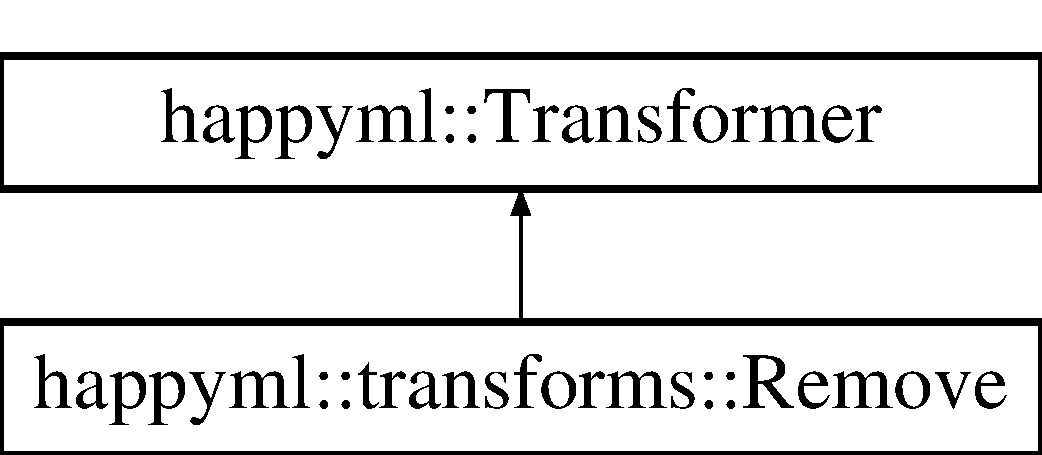
\includegraphics[height=2.000000cm]{classhappyml_1_1transforms_1_1Remove}
\end{center}
\end{figure}
\subsection*{Public Member Functions}
\begin{DoxyCompactItemize}
\item 
\hyperlink{classhappyml_1_1transforms_1_1Remove_a4b57c4b43e1d41229faec756ec3d66d5}{Remove} (int f)
\item 
void \hyperlink{classhappyml_1_1transforms_1_1Remove_a901c9a5c55f4b360233b8ba7e46fc198}{apply} (\hyperlink{classhappyml_1_1DataSet}{Data\+Set} \&dataset) const 
\begin{DoxyCompactList}\small\item\em Applies all the transformations at the given dataset. \end{DoxyCompactList}\item 
\hyperlink{namespacehappyml_a03602d1ec49393790b8a0449f40cd01f}{Input} \hyperlink{classhappyml_1_1transforms_1_1Remove_a249eec291d4c15b4e8e044c38a994770}{apply} (const \hyperlink{namespacehappyml_a03602d1ec49393790b8a0449f40cd01f}{Input} \&input) const 
\begin{DoxyCompactList}\small\item\em Applies all the transformations at the given input. \end{DoxyCompactList}\item 
void \hyperlink{classhappyml_1_1transforms_1_1Remove_a4f939046d630fa525dcc6d406b66e5b6}{apply} (mat \&x) const 
\end{DoxyCompactItemize}
\subsection*{Protected Attributes}
\begin{DoxyCompactItemize}
\item 
int \hyperlink{classhappyml_1_1transforms_1_1Remove_a4fbe1173bd54762002025be350dd13d5}{feature}
\end{DoxyCompactItemize}


\subsection{Constructor \& Destructor Documentation}
\index{happyml\+::transforms\+::\+Remove@{happyml\+::transforms\+::\+Remove}!Remove@{Remove}}
\index{Remove@{Remove}!happyml\+::transforms\+::\+Remove@{happyml\+::transforms\+::\+Remove}}
\subsubsection[{\texorpdfstring{Remove(int f)}{Remove(int f)}}]{\setlength{\rightskip}{0pt plus 5cm}happyml\+::transforms\+::\+Remove\+::\+Remove (
\begin{DoxyParamCaption}
\item[{int}]{f}
\end{DoxyParamCaption}
)\hspace{0.3cm}{\ttfamily [inline]}}\hypertarget{classhappyml_1_1transforms_1_1Remove_a4b57c4b43e1d41229faec756ec3d66d5}{}\label{classhappyml_1_1transforms_1_1Remove_a4b57c4b43e1d41229faec756ec3d66d5}


\subsection{Member Function Documentation}
\index{happyml\+::transforms\+::\+Remove@{happyml\+::transforms\+::\+Remove}!apply@{apply}}
\index{apply@{apply}!happyml\+::transforms\+::\+Remove@{happyml\+::transforms\+::\+Remove}}
\subsubsection[{\texorpdfstring{apply(\+Data\+Set \&dataset) const }{apply(DataSet &dataset) const }}]{\setlength{\rightskip}{0pt plus 5cm}void happyml\+::transforms\+::\+Remove\+::apply (
\begin{DoxyParamCaption}
\item[{{\bf Data\+Set} \&}]{dataset}
\end{DoxyParamCaption}
) const\hspace{0.3cm}{\ttfamily [virtual]}}\hypertarget{classhappyml_1_1transforms_1_1Remove_a901c9a5c55f4b360233b8ba7e46fc198}{}\label{classhappyml_1_1transforms_1_1Remove_a901c9a5c55f4b360233b8ba7e46fc198}


Applies all the transformations at the given dataset. 


\begin{DoxyParams}{Parameters}
{\em dataset} & Dataset to transform. \\
\hline
\end{DoxyParams}


Reimplemented from \hyperlink{classhappyml_1_1Transformer_a169a2a8434124c1dd8e671bca2cfa71d}{happyml\+::\+Transformer}.

\index{happyml\+::transforms\+::\+Remove@{happyml\+::transforms\+::\+Remove}!apply@{apply}}
\index{apply@{apply}!happyml\+::transforms\+::\+Remove@{happyml\+::transforms\+::\+Remove}}
\subsubsection[{\texorpdfstring{apply(const Input \&input) const }{apply(const Input &input) const }}]{\setlength{\rightskip}{0pt plus 5cm}{\bf Input} happyml\+::transforms\+::\+Remove\+::apply (
\begin{DoxyParamCaption}
\item[{const {\bf Input} \&}]{input}
\end{DoxyParamCaption}
) const\hspace{0.3cm}{\ttfamily [virtual]}}\hypertarget{classhappyml_1_1transforms_1_1Remove_a249eec291d4c15b4e8e044c38a994770}{}\label{classhappyml_1_1transforms_1_1Remove_a249eec291d4c15b4e8e044c38a994770}


Applies all the transformations at the given input. 


\begin{DoxyParams}{Parameters}
{\em input} & Input to transform.\\
\hline
\end{DoxyParams}
\begin{DoxyReturn}{Returns}
A transformated version of the input. 
\end{DoxyReturn}


Reimplemented from \hyperlink{classhappyml_1_1Transformer_a3e0eb67990c90c461466307fdefab45c}{happyml\+::\+Transformer}.

\index{happyml\+::transforms\+::\+Remove@{happyml\+::transforms\+::\+Remove}!apply@{apply}}
\index{apply@{apply}!happyml\+::transforms\+::\+Remove@{happyml\+::transforms\+::\+Remove}}
\subsubsection[{\texorpdfstring{apply(mat \&x) const }{apply(mat &x) const }}]{\setlength{\rightskip}{0pt plus 5cm}void happyml\+::transforms\+::\+Remove\+::apply (
\begin{DoxyParamCaption}
\item[{mat \&}]{x}
\end{DoxyParamCaption}
) const}\hypertarget{classhappyml_1_1transforms_1_1Remove_a4f939046d630fa525dcc6d406b66e5b6}{}\label{classhappyml_1_1transforms_1_1Remove_a4f939046d630fa525dcc6d406b66e5b6}


\subsection{Member Data Documentation}
\index{happyml\+::transforms\+::\+Remove@{happyml\+::transforms\+::\+Remove}!feature@{feature}}
\index{feature@{feature}!happyml\+::transforms\+::\+Remove@{happyml\+::transforms\+::\+Remove}}
\subsubsection[{\texorpdfstring{feature}{feature}}]{\setlength{\rightskip}{0pt plus 5cm}int happyml\+::transforms\+::\+Remove\+::feature\hspace{0.3cm}{\ttfamily [protected]}}\hypertarget{classhappyml_1_1transforms_1_1Remove_a4fbe1173bd54762002025be350dd13d5}{}\label{classhappyml_1_1transforms_1_1Remove_a4fbe1173bd54762002025be350dd13d5}


The documentation for this class was generated from the following files\+:\begin{DoxyCompactItemize}
\item 
include/happyml/transformers/\hyperlink{transformer_8h}{transformer.\+h}\item 
src/transformers/\hyperlink{transformer_8cpp}{transformer.\+cpp}\end{DoxyCompactItemize}

\hypertarget{classhappyml_1_1Serializable}{}\section{happyml\+:\+:Serializable Class Reference}
\label{classhappyml_1_1Serializable}\index{happyml\+::\+Serializable@{happyml\+::\+Serializable}}


Abstract class that represent an object that can be loaded from a file and saved to a file.  




{\ttfamily \#include $<$serializable.\+h$>$}

Inheritance diagram for happyml\+:\+:Serializable\+:\begin{figure}[H]
\begin{center}
\leavevmode
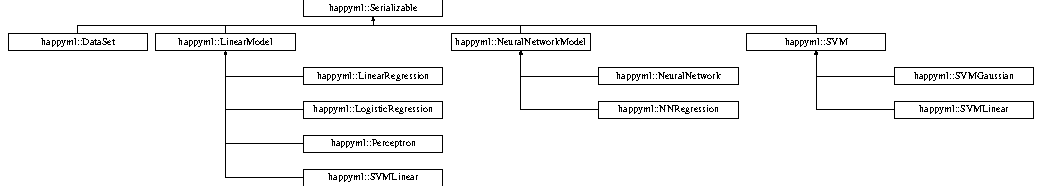
\includegraphics[height=2.500000cm]{classhappyml_1_1Serializable}
\end{center}
\end{figure}
\subsection*{Public Member Functions}
\begin{DoxyCompactItemize}
\item 
virtual void \hyperlink{classhappyml_1_1Serializable_a839f14e831098c5c9ffd1ce149df71b3}{load} (const string \&filename)
\begin{DoxyCompactList}\small\item\em Fills an object using the data in the given file. \end{DoxyCompactList}\item 
virtual void \hyperlink{classhappyml_1_1Serializable_a06a0a44a24b1c800115875b44d07cff9}{save} (const string \&filename) const 
\begin{DoxyCompactList}\small\item\em Saves the object to a specific file. \end{DoxyCompactList}\item 
virtual void \hyperlink{classhappyml_1_1Serializable_aef5c211d8e9c1c425b33c657824c2f0c}{read} (istream \&stream)=0
\begin{DoxyCompactList}\small\item\em Read the object from an input stream. \end{DoxyCompactList}\item 
virtual void \hyperlink{classhappyml_1_1Serializable_a2d503e4c2e39c5be8a33bcc8b691949f}{write} (ostream \&stream) const  =0
\begin{DoxyCompactList}\small\item\em Write the object to an output stream. \end{DoxyCompactList}\end{DoxyCompactItemize}


\subsection{Detailed Description}
Abstract class that represent an object that can be loaded from a file and saved to a file. 

\subsection{Member Function Documentation}
\index{happyml\+::\+Serializable@{happyml\+::\+Serializable}!load@{load}}
\index{load@{load}!happyml\+::\+Serializable@{happyml\+::\+Serializable}}
\subsubsection[{\texorpdfstring{load(const string \&filename)}{load(const string &filename)}}]{\setlength{\rightskip}{0pt plus 5cm}void happyml\+::\+Serializable\+::load (
\begin{DoxyParamCaption}
\item[{const string \&}]{filename}
\end{DoxyParamCaption}
)\hspace{0.3cm}{\ttfamily [virtual]}}\hypertarget{classhappyml_1_1Serializable_a839f14e831098c5c9ffd1ce149df71b3}{}\label{classhappyml_1_1Serializable_a839f14e831098c5c9ffd1ce149df71b3}


Fills an object using the data in the given file. 


\begin{DoxyParams}{Parameters}
{\em filename} & Name of the file to load.\\
\hline
\end{DoxyParams}
\begin{DoxySeeAlso}{See also}
save(const string\&) 
\end{DoxySeeAlso}
\index{happyml\+::\+Serializable@{happyml\+::\+Serializable}!read@{read}}
\index{read@{read}!happyml\+::\+Serializable@{happyml\+::\+Serializable}}
\subsubsection[{\texorpdfstring{read(istream \&stream)=0}{read(istream &stream)=0}}]{\setlength{\rightskip}{0pt plus 5cm}virtual void happyml\+::\+Serializable\+::read (
\begin{DoxyParamCaption}
\item[{istream \&}]{stream}
\end{DoxyParamCaption}
)\hspace{0.3cm}{\ttfamily [pure virtual]}}\hypertarget{classhappyml_1_1Serializable_aef5c211d8e9c1c425b33c657824c2f0c}{}\label{classhappyml_1_1Serializable_aef5c211d8e9c1c425b33c657824c2f0c}


Read the object from an input stream. 


\begin{DoxyParams}{Parameters}
{\em stream} & Input stream. \\
\hline
\end{DoxyParams}


Implemented in \hyperlink{classhappyml_1_1NeuralNetworkModel_a5591e0392dc1ec3d6d730ae355cc7f09}{happyml\+::\+Neural\+Network\+Model}, \hyperlink{classhappyml_1_1DataSet_aa2e2f9c87aefbf9c7a2b8793f197b828}{happyml\+::\+Data\+Set}, \hyperlink{classhappyml_1_1SVM_a180e169777af513b76cada99044ad3c3}{happyml\+::\+S\+VM}, \hyperlink{classhappyml_1_1LinearModel_abdc75a19c7234d8bc13b4dd7ad621c9e}{happyml\+::\+Linear\+Model}, and \hyperlink{classhappyml_1_1SVMLinear_a4259c29ba1acd320703bf8c1ae8fd780}{happyml\+::\+S\+V\+M\+Linear}.

\index{happyml\+::\+Serializable@{happyml\+::\+Serializable}!save@{save}}
\index{save@{save}!happyml\+::\+Serializable@{happyml\+::\+Serializable}}
\subsubsection[{\texorpdfstring{save(const string \&filename) const }{save(const string &filename) const }}]{\setlength{\rightskip}{0pt plus 5cm}void happyml\+::\+Serializable\+::save (
\begin{DoxyParamCaption}
\item[{const string \&}]{filename}
\end{DoxyParamCaption}
) const\hspace{0.3cm}{\ttfamily [virtual]}}\hypertarget{classhappyml_1_1Serializable_a06a0a44a24b1c800115875b44d07cff9}{}\label{classhappyml_1_1Serializable_a06a0a44a24b1c800115875b44d07cff9}


Saves the object to a specific file. 

After this call you can load new objects using the load method and that filename.


\begin{DoxyParams}{Parameters}
{\em filename} & Output filename.\\
\hline
\end{DoxyParams}
\begin{DoxySeeAlso}{See also}
\hyperlink{classhappyml_1_1Serializable_a839f14e831098c5c9ffd1ce149df71b3}{load(const string\&)} 
\end{DoxySeeAlso}
\index{happyml\+::\+Serializable@{happyml\+::\+Serializable}!write@{write}}
\index{write@{write}!happyml\+::\+Serializable@{happyml\+::\+Serializable}}
\subsubsection[{\texorpdfstring{write(ostream \&stream) const  =0}{write(ostream &stream) const  =0}}]{\setlength{\rightskip}{0pt plus 5cm}virtual void happyml\+::\+Serializable\+::write (
\begin{DoxyParamCaption}
\item[{ostream \&}]{stream}
\end{DoxyParamCaption}
) const\hspace{0.3cm}{\ttfamily [pure virtual]}}\hypertarget{classhappyml_1_1Serializable_a2d503e4c2e39c5be8a33bcc8b691949f}{}\label{classhappyml_1_1Serializable_a2d503e4c2e39c5be8a33bcc8b691949f}


Write the object to an output stream. 


\begin{DoxyParams}{Parameters}
{\em stream} & Output stream. \\
\hline
\end{DoxyParams}


Implemented in \hyperlink{classhappyml_1_1NeuralNetworkModel_acaae169ac128c0c707342960e7c048eb}{happyml\+::\+Neural\+Network\+Model}, \hyperlink{classhappyml_1_1DataSet_a1bed7d89826c5b9fb23c3e2d0f690b22}{happyml\+::\+Data\+Set}, \hyperlink{classhappyml_1_1LinearModel_ad788fb6f13ba64d8164a89a8be96949d}{happyml\+::\+Linear\+Model}, and \hyperlink{classhappyml_1_1SVM_a71cdc4e06322b9555dbcc118b45c4f73}{happyml\+::\+S\+VM}.



The documentation for this class was generated from the following files\+:\begin{DoxyCompactItemize}
\item 
include/happyml/\hyperlink{serializable_8h}{serializable.\+h}\item 
src/\hyperlink{serializable_8cpp}{serializable.\+cpp}\end{DoxyCompactItemize}

\hypertarget{classhappyml_1_1transforms_1_1SimpleTransformer}{}\section{happyml\+:\+:transforms\+:\+:Simple\+Transformer Class Reference}
\label{classhappyml_1_1transforms_1_1SimpleTransformer}\index{happyml\+::transforms\+::\+Simple\+Transformer@{happyml\+::transforms\+::\+Simple\+Transformer}}


{\ttfamily \#include $<$transformer.\+h$>$}

Inheritance diagram for happyml\+:\+:transforms\+:\+:Simple\+Transformer\+:\begin{figure}[H]
\begin{center}
\leavevmode
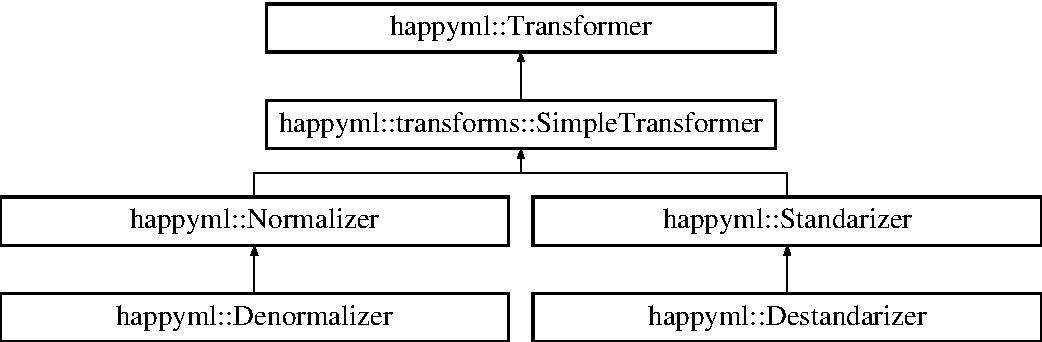
\includegraphics[height=4.000000cm]{classhappyml_1_1transforms_1_1SimpleTransformer}
\end{center}
\end{figure}
\subsection*{Public Member Functions}
\begin{DoxyCompactItemize}
\item 
\hyperlink{classhappyml_1_1transforms_1_1SimpleTransformer_aab5bd97120b0370e6fb6df1ed86f5483}{Simple\+Transformer} ()
\item 
void \hyperlink{classhappyml_1_1transforms_1_1SimpleTransformer_a7bb7863c5f6b2e0a36eac155b1f25cdf}{apply} (\hyperlink{classhappyml_1_1DataSet}{Data\+Set} \&dataset) const 
\begin{DoxyCompactList}\small\item\em Applies all the transformations at the given dataset. \end{DoxyCompactList}\item 
\hyperlink{namespacehappyml_a03602d1ec49393790b8a0449f40cd01f}{Input} \hyperlink{classhappyml_1_1transforms_1_1SimpleTransformer_a27df37bea3d873ec44ad819db60c523e}{apply} (const \hyperlink{namespacehappyml_a03602d1ec49393790b8a0449f40cd01f}{Input} \&input, bool has\+X0=true) const 
\item 
virtual void \hyperlink{classhappyml_1_1transforms_1_1SimpleTransformer_a2f38b1b4eb85dca83cb9f6ed9796da32}{apply} (mat \&x) const 
\end{DoxyCompactItemize}


\subsection{Constructor \& Destructor Documentation}
\index{happyml\+::transforms\+::\+Simple\+Transformer@{happyml\+::transforms\+::\+Simple\+Transformer}!Simple\+Transformer@{Simple\+Transformer}}
\index{Simple\+Transformer@{Simple\+Transformer}!happyml\+::transforms\+::\+Simple\+Transformer@{happyml\+::transforms\+::\+Simple\+Transformer}}
\subsubsection[{\texorpdfstring{Simple\+Transformer()}{SimpleTransformer()}}]{\setlength{\rightskip}{0pt plus 5cm}happyml\+::transforms\+::\+Simple\+Transformer\+::\+Simple\+Transformer (
\begin{DoxyParamCaption}
{}
\end{DoxyParamCaption}
)\hspace{0.3cm}{\ttfamily [inline]}}\hypertarget{classhappyml_1_1transforms_1_1SimpleTransformer_aab5bd97120b0370e6fb6df1ed86f5483}{}\label{classhappyml_1_1transforms_1_1SimpleTransformer_aab5bd97120b0370e6fb6df1ed86f5483}


\subsection{Member Function Documentation}
\index{happyml\+::transforms\+::\+Simple\+Transformer@{happyml\+::transforms\+::\+Simple\+Transformer}!apply@{apply}}
\index{apply@{apply}!happyml\+::transforms\+::\+Simple\+Transformer@{happyml\+::transforms\+::\+Simple\+Transformer}}
\subsubsection[{\texorpdfstring{apply(\+Data\+Set \&dataset) const }{apply(DataSet &dataset) const }}]{\setlength{\rightskip}{0pt plus 5cm}void happyml\+::transforms\+::\+Simple\+Transformer\+::apply (
\begin{DoxyParamCaption}
\item[{{\bf Data\+Set} \&}]{dataset}
\end{DoxyParamCaption}
) const\hspace{0.3cm}{\ttfamily [virtual]}}\hypertarget{classhappyml_1_1transforms_1_1SimpleTransformer_a7bb7863c5f6b2e0a36eac155b1f25cdf}{}\label{classhappyml_1_1transforms_1_1SimpleTransformer_a7bb7863c5f6b2e0a36eac155b1f25cdf}


Applies all the transformations at the given dataset. 


\begin{DoxyParams}{Parameters}
{\em dataset} & Dataset to transform. \\
\hline
\end{DoxyParams}


Reimplemented from \hyperlink{classhappyml_1_1Transformer_a169a2a8434124c1dd8e671bca2cfa71d}{happyml\+::\+Transformer}.

\index{happyml\+::transforms\+::\+Simple\+Transformer@{happyml\+::transforms\+::\+Simple\+Transformer}!apply@{apply}}
\index{apply@{apply}!happyml\+::transforms\+::\+Simple\+Transformer@{happyml\+::transforms\+::\+Simple\+Transformer}}
\subsubsection[{\texorpdfstring{apply(const Input \&input, bool has\+X0=true) const }{apply(const Input &input, bool hasX0=true) const }}]{\setlength{\rightskip}{0pt plus 5cm}{\bf Input} happyml\+::transforms\+::\+Simple\+Transformer\+::apply (
\begin{DoxyParamCaption}
\item[{const {\bf Input} \&}]{input, }
\item[{bool}]{has\+X0 = {\ttfamily true}}
\end{DoxyParamCaption}
) const}\hypertarget{classhappyml_1_1transforms_1_1SimpleTransformer_a27df37bea3d873ec44ad819db60c523e}{}\label{classhappyml_1_1transforms_1_1SimpleTransformer_a27df37bea3d873ec44ad819db60c523e}
\index{happyml\+::transforms\+::\+Simple\+Transformer@{happyml\+::transforms\+::\+Simple\+Transformer}!apply@{apply}}
\index{apply@{apply}!happyml\+::transforms\+::\+Simple\+Transformer@{happyml\+::transforms\+::\+Simple\+Transformer}}
\subsubsection[{\texorpdfstring{apply(mat \&x) const }{apply(mat &x) const }}]{\setlength{\rightskip}{0pt plus 5cm}virtual void happyml\+::transforms\+::\+Simple\+Transformer\+::apply (
\begin{DoxyParamCaption}
\item[{mat \&}]{x}
\end{DoxyParamCaption}
) const\hspace{0.3cm}{\ttfamily [inline]}, {\ttfamily [virtual]}}\hypertarget{classhappyml_1_1transforms_1_1SimpleTransformer_a2f38b1b4eb85dca83cb9f6ed9796da32}{}\label{classhappyml_1_1transforms_1_1SimpleTransformer_a2f38b1b4eb85dca83cb9f6ed9796da32}


Reimplemented in \hyperlink{classhappyml_1_1Denormalizer_a2f1aa35006d0573f07fc33e8f154c170}{happyml\+::\+Denormalizer}, \hyperlink{classhappyml_1_1Destandarizer_a2d1542f1857bfe0cb23fa69b139d2368}{happyml\+::\+Destandarizer}, \hyperlink{classhappyml_1_1Normalizer_aeff0b4e117d69311cc5845c9915fa691}{happyml\+::\+Normalizer}, and \hyperlink{classhappyml_1_1Standarizer_a5c9b416b657cb61972c27b27fd379b2d}{happyml\+::\+Standarizer}.



The documentation for this class was generated from the following files\+:\begin{DoxyCompactItemize}
\item 
include/happyml/transformers/\hyperlink{transformer_8h}{transformer.\+h}\item 
src/transformers/\hyperlink{transformer_8cpp}{transformer.\+cpp}\end{DoxyCompactItemize}

\hypertarget{classhappyml_1_1Standarizer}{}\section{happyml\+:\+:Standarizer Class Reference}
\label{classhappyml_1_1Standarizer}\index{happyml\+::\+Standarizer@{happyml\+::\+Standarizer}}


Applies Z-\/\+Score transformation\+: x\textquotesingle{} = x -\/ mean(x) / stddev(x)  




{\ttfamily \#include $<$standarizer.\+h$>$}

Inheritance diagram for happyml\+:\+:Standarizer\+:\begin{figure}[H]
\begin{center}
\leavevmode
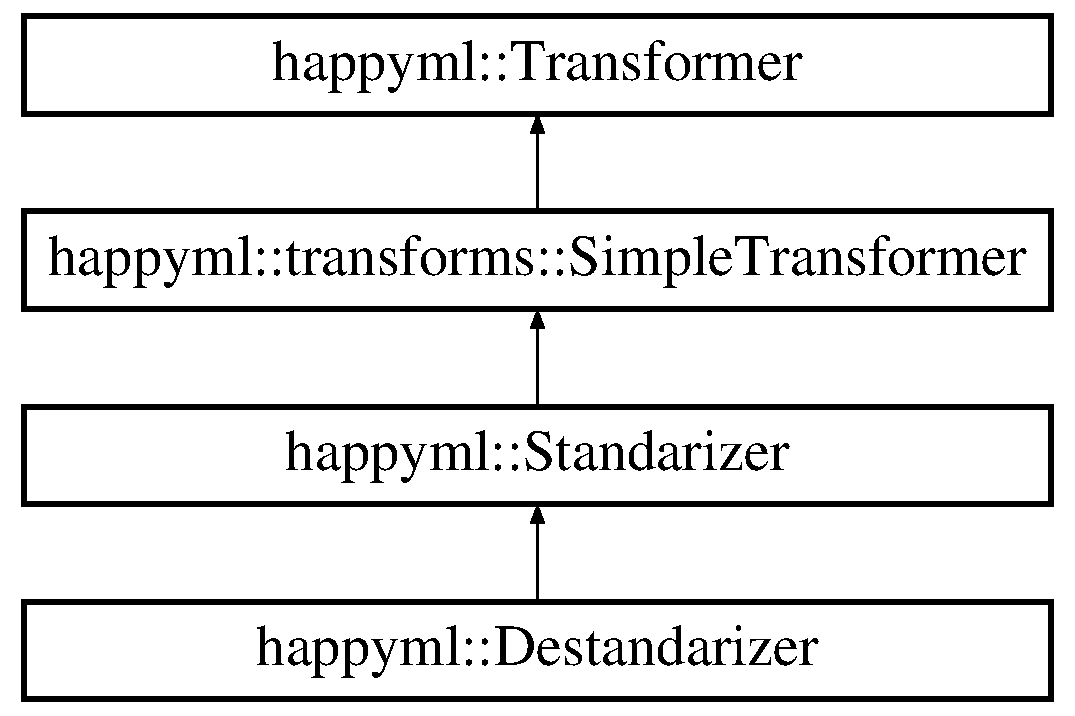
\includegraphics[height=4.000000cm]{classhappyml_1_1Standarizer}
\end{center}
\end{figure}
\subsection*{Public Member Functions}
\begin{DoxyCompactItemize}
\item 
\hyperlink{classhappyml_1_1Standarizer_a017f97c038070ab78c0c7d0e4fd3dc96}{Standarizer} (const \hyperlink{classhappyml_1_1DataSet}{Data\+Set} \&dataset)
\begin{DoxyCompactList}\small\item\em Creates a standarizer that will use mean and stddev data obtained from the dataset. \end{DoxyCompactList}\item 
\hyperlink{classhappyml_1_1Standarizer_ac0c6d451821afef5832cae79e28edf35}{Standarizer} (const mat \&x)
\begin{DoxyCompactList}\small\item\em Creates a standarizer that will use mean and stddev data obtained from the given matrix. \end{DoxyCompactList}\item 
\hyperlink{classhappyml_1_1Standarizer_a5b69e125c31e779feaf00d30109dd576}{Standarizer} (vec mean, vec stddev)
\begin{DoxyCompactList}\small\item\em Creates a standarizer that will use mean and stddev vectors. \end{DoxyCompactList}\item 
\hyperlink{classhappyml_1_1Standarizer_aa603e5cce8b82997914cf9d1fe67cd88}{$\sim$\+Standarizer} ()
\item 
void \hyperlink{classhappyml_1_1Standarizer_a5c9b416b657cb61972c27b27fd379b2d}{apply} (mat \&x) const 
\end{DoxyCompactItemize}
\subsection*{Protected Member Functions}
\begin{DoxyCompactItemize}
\item 
void \hyperlink{classhappyml_1_1Standarizer_abe4eda61396072e6fb43f92708b6b9ea}{init} (const mat \&)
\end{DoxyCompactItemize}
\subsection*{Protected Attributes}
\begin{DoxyCompactItemize}
\item 
rowvec \hyperlink{classhappyml_1_1Standarizer_a944bac3d123e8e849b29a684b8231711}{mean\+Vec}
\item 
rowvec \hyperlink{classhappyml_1_1Standarizer_a06db5ac6fc3d3c75a26be5c266f7af94}{std\+Vec}
\end{DoxyCompactItemize}


\subsection{Detailed Description}
Applies Z-\/\+Score transformation\+: x\textquotesingle{} = x -\/ mean(x) / stddev(x) 

\subsection{Constructor \& Destructor Documentation}
\index{happyml\+::\+Standarizer@{happyml\+::\+Standarizer}!Standarizer@{Standarizer}}
\index{Standarizer@{Standarizer}!happyml\+::\+Standarizer@{happyml\+::\+Standarizer}}
\subsubsection[{\texorpdfstring{Standarizer(const Data\+Set \&dataset)}{Standarizer(const DataSet &dataset)}}]{\setlength{\rightskip}{0pt plus 5cm}happyml\+::\+Standarizer\+::\+Standarizer (
\begin{DoxyParamCaption}
\item[{const {\bf Data\+Set} \&}]{dataset}
\end{DoxyParamCaption}
)\hspace{0.3cm}{\ttfamily [inline]}}\hypertarget{classhappyml_1_1Standarizer_a017f97c038070ab78c0c7d0e4fd3dc96}{}\label{classhappyml_1_1Standarizer_a017f97c038070ab78c0c7d0e4fd3dc96}


Creates a standarizer that will use mean and stddev data obtained from the dataset. 


\begin{DoxyParams}{Parameters}
{\em dataset} & Dataset from which it will be extracted the mean and stddev that will be used when apply Z-\/\+Score. //\\
\hline
{\em normY} & If true, it standarizes also the outputs. \\
\hline
\end{DoxyParams}
\index{happyml\+::\+Standarizer@{happyml\+::\+Standarizer}!Standarizer@{Standarizer}}
\index{Standarizer@{Standarizer}!happyml\+::\+Standarizer@{happyml\+::\+Standarizer}}
\subsubsection[{\texorpdfstring{Standarizer(const mat \&x)}{Standarizer(const mat &x)}}]{\setlength{\rightskip}{0pt plus 5cm}happyml\+::\+Standarizer\+::\+Standarizer (
\begin{DoxyParamCaption}
\item[{const mat \&}]{x}
\end{DoxyParamCaption}
)\hspace{0.3cm}{\ttfamily [inline]}}\hypertarget{classhappyml_1_1Standarizer_ac0c6d451821afef5832cae79e28edf35}{}\label{classhappyml_1_1Standarizer_ac0c6d451821afef5832cae79e28edf35}


Creates a standarizer that will use mean and stddev data obtained from the given matrix. 


\begin{DoxyParams}{Parameters}
{\em x} & Matrix from which it will be extracted the mean and stddev vectors that will be used when apply Z-\/\+Score. \\
\hline
\end{DoxyParams}
\index{happyml\+::\+Standarizer@{happyml\+::\+Standarizer}!Standarizer@{Standarizer}}
\index{Standarizer@{Standarizer}!happyml\+::\+Standarizer@{happyml\+::\+Standarizer}}
\subsubsection[{\texorpdfstring{Standarizer(vec mean, vec stddev)}{Standarizer(vec mean, vec stddev)}}]{\setlength{\rightskip}{0pt plus 5cm}happyml\+::\+Standarizer\+::\+Standarizer (
\begin{DoxyParamCaption}
\item[{vec}]{mean, }
\item[{vec}]{stddev}
\end{DoxyParamCaption}
)\hspace{0.3cm}{\ttfamily [inline]}}\hypertarget{classhappyml_1_1Standarizer_a5b69e125c31e779feaf00d30109dd576}{}\label{classhappyml_1_1Standarizer_a5b69e125c31e779feaf00d30109dd576}


Creates a standarizer that will use mean and stddev vectors. 


\begin{DoxyParams}{Parameters}
{\em mean} & Vector with the mean of each column. \\
\hline
{\em stddev} & Vector with the stddev of each column. \\
\hline
\end{DoxyParams}
\index{happyml\+::\+Standarizer@{happyml\+::\+Standarizer}!````~Standarizer@{$\sim$\+Standarizer}}
\index{````~Standarizer@{$\sim$\+Standarizer}!happyml\+::\+Standarizer@{happyml\+::\+Standarizer}}
\subsubsection[{\texorpdfstring{$\sim$\+Standarizer()}{~Standarizer()}}]{\setlength{\rightskip}{0pt plus 5cm}happyml\+::\+Standarizer\+::$\sim$\+Standarizer (
\begin{DoxyParamCaption}
{}
\end{DoxyParamCaption}
)\hspace{0.3cm}{\ttfamily [inline]}}\hypertarget{classhappyml_1_1Standarizer_aa603e5cce8b82997914cf9d1fe67cd88}{}\label{classhappyml_1_1Standarizer_aa603e5cce8b82997914cf9d1fe67cd88}


\subsection{Member Function Documentation}
\index{happyml\+::\+Standarizer@{happyml\+::\+Standarizer}!apply@{apply}}
\index{apply@{apply}!happyml\+::\+Standarizer@{happyml\+::\+Standarizer}}
\subsubsection[{\texorpdfstring{apply(mat \&x) const }{apply(mat &x) const }}]{\setlength{\rightskip}{0pt plus 5cm}void happyml\+::\+Standarizer\+::apply (
\begin{DoxyParamCaption}
\item[{mat \&}]{x}
\end{DoxyParamCaption}
) const\hspace{0.3cm}{\ttfamily [virtual]}}\hypertarget{classhappyml_1_1Standarizer_a5c9b416b657cb61972c27b27fd379b2d}{}\label{classhappyml_1_1Standarizer_a5c9b416b657cb61972c27b27fd379b2d}


Reimplemented from \hyperlink{classhappyml_1_1transforms_1_1SimpleTransformer_a2f38b1b4eb85dca83cb9f6ed9796da32}{happyml\+::transforms\+::\+Simple\+Transformer}.



Reimplemented in \hyperlink{classhappyml_1_1Destandarizer_a2d1542f1857bfe0cb23fa69b139d2368}{happyml\+::\+Destandarizer}.

\index{happyml\+::\+Standarizer@{happyml\+::\+Standarizer}!init@{init}}
\index{init@{init}!happyml\+::\+Standarizer@{happyml\+::\+Standarizer}}
\subsubsection[{\texorpdfstring{init(const mat \&)}{init(const mat &)}}]{\setlength{\rightskip}{0pt plus 5cm}void happyml\+::\+Standarizer\+::init (
\begin{DoxyParamCaption}
\item[{const mat \&}]{x}
\end{DoxyParamCaption}
)\hspace{0.3cm}{\ttfamily [protected]}}\hypertarget{classhappyml_1_1Standarizer_abe4eda61396072e6fb43f92708b6b9ea}{}\label{classhappyml_1_1Standarizer_abe4eda61396072e6fb43f92708b6b9ea}


\subsection{Member Data Documentation}
\index{happyml\+::\+Standarizer@{happyml\+::\+Standarizer}!mean\+Vec@{mean\+Vec}}
\index{mean\+Vec@{mean\+Vec}!happyml\+::\+Standarizer@{happyml\+::\+Standarizer}}
\subsubsection[{\texorpdfstring{mean\+Vec}{meanVec}}]{\setlength{\rightskip}{0pt plus 5cm}rowvec happyml\+::\+Standarizer\+::mean\+Vec\hspace{0.3cm}{\ttfamily [protected]}}\hypertarget{classhappyml_1_1Standarizer_a944bac3d123e8e849b29a684b8231711}{}\label{classhappyml_1_1Standarizer_a944bac3d123e8e849b29a684b8231711}
\index{happyml\+::\+Standarizer@{happyml\+::\+Standarizer}!std\+Vec@{std\+Vec}}
\index{std\+Vec@{std\+Vec}!happyml\+::\+Standarizer@{happyml\+::\+Standarizer}}
\subsubsection[{\texorpdfstring{std\+Vec}{stdVec}}]{\setlength{\rightskip}{0pt plus 5cm}rowvec happyml\+::\+Standarizer\+::std\+Vec\hspace{0.3cm}{\ttfamily [protected]}}\hypertarget{classhappyml_1_1Standarizer_a06db5ac6fc3d3c75a26be5c266f7af94}{}\label{classhappyml_1_1Standarizer_a06db5ac6fc3d3c75a26be5c266f7af94}


The documentation for this class was generated from the following files\+:\begin{DoxyCompactItemize}
\item 
include/happyml/transformers/\hyperlink{standarizer_8h}{standarizer.\+h}\item 
src/transformers/\hyperlink{standarizer_8cpp}{standarizer.\+cpp}\end{DoxyCompactItemize}

\hypertarget{classhappyml_1_1StandarizerXY}{}\section{happyml\+:\+:Standarizer\+XY Class Reference}
\label{classhappyml_1_1StandarizerXY}\index{happyml\+::\+Standarizer\+XY@{happyml\+::\+Standarizer\+XY}}


{\ttfamily \#include $<$standarizer.\+h$>$}

Inheritance diagram for happyml\+:\+:Standarizer\+XY\+:\begin{figure}[H]
\begin{center}
\leavevmode
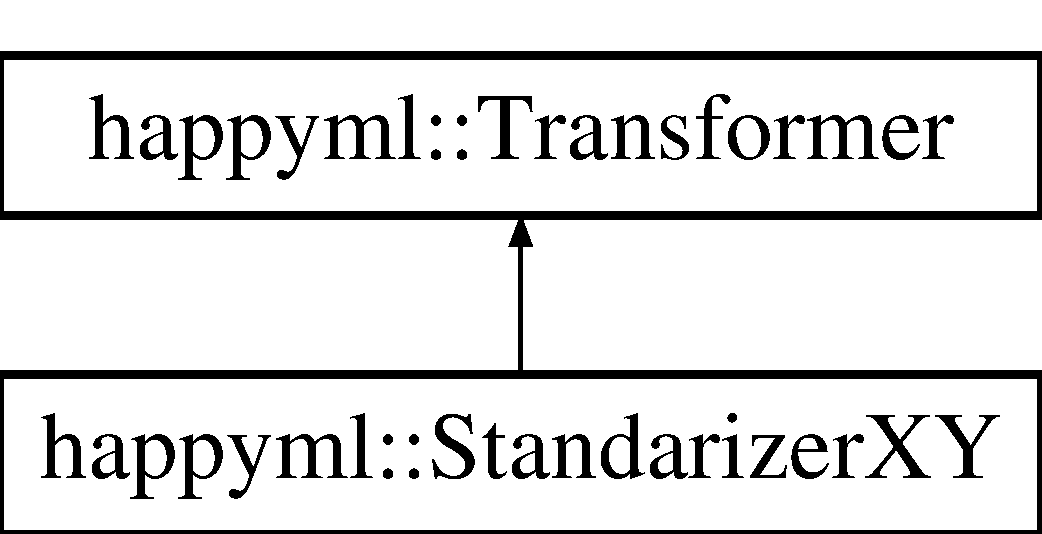
\includegraphics[height=2.000000cm]{classhappyml_1_1StandarizerXY}
\end{center}
\end{figure}
\subsection*{Public Member Functions}
\begin{DoxyCompactItemize}
\item 
\hyperlink{classhappyml_1_1StandarizerXY_a49f04a43ba7eff7fbb5694ee7b291f1b}{Standarizer\+XY} (const \hyperlink{classhappyml_1_1DataSet}{Data\+Set} \&d)
\item 
\hyperlink{classhappyml_1_1Standarizer}{Standarizer} \hyperlink{classhappyml_1_1StandarizerXY_ada7856e988a0e49d97ad49c7e5f2858f}{get\+StandarizerX} () const 
\item 
\hyperlink{classhappyml_1_1Standarizer}{Standarizer} \hyperlink{classhappyml_1_1StandarizerXY_a72864006fa4aa7cdf279921b7fbe397f}{get\+StandarizerY} () const 
\item 
void \hyperlink{classhappyml_1_1StandarizerXY_af2979980c88b3c5c4d670d2148c148e8}{apply} (\hyperlink{classhappyml_1_1DataSet}{Data\+Set} \&d) const 
\begin{DoxyCompactList}\small\item\em Applies all the transformations at the given dataset. \end{DoxyCompactList}\item 
\hyperlink{namespacehappyml_a03602d1ec49393790b8a0449f40cd01f}{Input} \hyperlink{classhappyml_1_1StandarizerXY_a800a8953dbf96c26edca660680ce791f}{apply} (const \hyperlink{namespacehappyml_a03602d1ec49393790b8a0449f40cd01f}{Input} \&input) const 
\begin{DoxyCompactList}\small\item\em Applies all the transformations at the given input. \end{DoxyCompactList}\item 
vec \hyperlink{classhappyml_1_1StandarizerXY_af42c8a94bd29b9e75b6deb770a391460}{apply\+Output} (const vec \&output) const 
\end{DoxyCompactItemize}
\subsection*{Protected Attributes}
\begin{DoxyCompactItemize}
\item 
\hyperlink{classhappyml_1_1Standarizer}{Standarizer} \hyperlink{classhappyml_1_1StandarizerXY_a5fa58f435e964fb2399250ff20bb9333}{nx}
\item 
\hyperlink{classhappyml_1_1Standarizer}{Standarizer} \hyperlink{classhappyml_1_1StandarizerXY_a0395628b7404fa30aafb7ecf9b2bf7cb}{ny}
\end{DoxyCompactItemize}
\subsection*{Friends}
\begin{DoxyCompactItemize}
\item 
class \hyperlink{classhappyml_1_1StandarizerXY_a685efff399e4806ec9c79de4c978b0df}{Destandarizer\+XY}
\end{DoxyCompactItemize}


\subsection{Constructor \& Destructor Documentation}
\index{happyml\+::\+Standarizer\+XY@{happyml\+::\+Standarizer\+XY}!Standarizer\+XY@{Standarizer\+XY}}
\index{Standarizer\+XY@{Standarizer\+XY}!happyml\+::\+Standarizer\+XY@{happyml\+::\+Standarizer\+XY}}
\subsubsection[{\texorpdfstring{Standarizer\+X\+Y(const Data\+Set \&d)}{StandarizerXY(const DataSet &d)}}]{\setlength{\rightskip}{0pt plus 5cm}happyml\+::\+Standarizer\+X\+Y\+::\+Standarizer\+XY (
\begin{DoxyParamCaption}
\item[{const {\bf Data\+Set} \&}]{d}
\end{DoxyParamCaption}
)\hspace{0.3cm}{\ttfamily [inline]}}\hypertarget{classhappyml_1_1StandarizerXY_a49f04a43ba7eff7fbb5694ee7b291f1b}{}\label{classhappyml_1_1StandarizerXY_a49f04a43ba7eff7fbb5694ee7b291f1b}


\subsection{Member Function Documentation}
\index{happyml\+::\+Standarizer\+XY@{happyml\+::\+Standarizer\+XY}!apply@{apply}}
\index{apply@{apply}!happyml\+::\+Standarizer\+XY@{happyml\+::\+Standarizer\+XY}}
\subsubsection[{\texorpdfstring{apply(\+Data\+Set \&d) const }{apply(DataSet &d) const }}]{\setlength{\rightskip}{0pt plus 5cm}void happyml\+::\+Standarizer\+X\+Y\+::apply (
\begin{DoxyParamCaption}
\item[{{\bf Data\+Set} \&}]{dataset}
\end{DoxyParamCaption}
) const\hspace{0.3cm}{\ttfamily [inline]}, {\ttfamily [virtual]}}\hypertarget{classhappyml_1_1StandarizerXY_af2979980c88b3c5c4d670d2148c148e8}{}\label{classhappyml_1_1StandarizerXY_af2979980c88b3c5c4d670d2148c148e8}


Applies all the transformations at the given dataset. 


\begin{DoxyParams}{Parameters}
{\em dataset} & Dataset to transform. \\
\hline
\end{DoxyParams}


Reimplemented from \hyperlink{classhappyml_1_1Transformer_a169a2a8434124c1dd8e671bca2cfa71d}{happyml\+::\+Transformer}.

\index{happyml\+::\+Standarizer\+XY@{happyml\+::\+Standarizer\+XY}!apply@{apply}}
\index{apply@{apply}!happyml\+::\+Standarizer\+XY@{happyml\+::\+Standarizer\+XY}}
\subsubsection[{\texorpdfstring{apply(const Input \&input) const }{apply(const Input &input) const }}]{\setlength{\rightskip}{0pt plus 5cm}{\bf Input} happyml\+::\+Standarizer\+X\+Y\+::apply (
\begin{DoxyParamCaption}
\item[{const {\bf Input} \&}]{input}
\end{DoxyParamCaption}
) const\hspace{0.3cm}{\ttfamily [inline]}, {\ttfamily [virtual]}}\hypertarget{classhappyml_1_1StandarizerXY_a800a8953dbf96c26edca660680ce791f}{}\label{classhappyml_1_1StandarizerXY_a800a8953dbf96c26edca660680ce791f}


Applies all the transformations at the given input. 


\begin{DoxyParams}{Parameters}
{\em input} & Input to transform.\\
\hline
\end{DoxyParams}
\begin{DoxyReturn}{Returns}
A transformated version of the input. 
\end{DoxyReturn}


Reimplemented from \hyperlink{classhappyml_1_1Transformer_a3e0eb67990c90c461466307fdefab45c}{happyml\+::\+Transformer}.

\index{happyml\+::\+Standarizer\+XY@{happyml\+::\+Standarizer\+XY}!apply\+Output@{apply\+Output}}
\index{apply\+Output@{apply\+Output}!happyml\+::\+Standarizer\+XY@{happyml\+::\+Standarizer\+XY}}
\subsubsection[{\texorpdfstring{apply\+Output(const vec \&output) const }{applyOutput(const vec &output) const }}]{\setlength{\rightskip}{0pt plus 5cm}vec happyml\+::\+Standarizer\+X\+Y\+::apply\+Output (
\begin{DoxyParamCaption}
\item[{const vec \&}]{output}
\end{DoxyParamCaption}
) const\hspace{0.3cm}{\ttfamily [inline]}}\hypertarget{classhappyml_1_1StandarizerXY_af42c8a94bd29b9e75b6deb770a391460}{}\label{classhappyml_1_1StandarizerXY_af42c8a94bd29b9e75b6deb770a391460}
\index{happyml\+::\+Standarizer\+XY@{happyml\+::\+Standarizer\+XY}!get\+StandarizerX@{get\+StandarizerX}}
\index{get\+StandarizerX@{get\+StandarizerX}!happyml\+::\+Standarizer\+XY@{happyml\+::\+Standarizer\+XY}}
\subsubsection[{\texorpdfstring{get\+Standarizer\+X() const }{getStandarizerX() const }}]{\setlength{\rightskip}{0pt plus 5cm}{\bf Standarizer} happyml\+::\+Standarizer\+X\+Y\+::get\+StandarizerX (
\begin{DoxyParamCaption}
{}
\end{DoxyParamCaption}
) const\hspace{0.3cm}{\ttfamily [inline]}}\hypertarget{classhappyml_1_1StandarizerXY_ada7856e988a0e49d97ad49c7e5f2858f}{}\label{classhappyml_1_1StandarizerXY_ada7856e988a0e49d97ad49c7e5f2858f}
\index{happyml\+::\+Standarizer\+XY@{happyml\+::\+Standarizer\+XY}!get\+StandarizerY@{get\+StandarizerY}}
\index{get\+StandarizerY@{get\+StandarizerY}!happyml\+::\+Standarizer\+XY@{happyml\+::\+Standarizer\+XY}}
\subsubsection[{\texorpdfstring{get\+Standarizer\+Y() const }{getStandarizerY() const }}]{\setlength{\rightskip}{0pt plus 5cm}{\bf Standarizer} happyml\+::\+Standarizer\+X\+Y\+::get\+StandarizerY (
\begin{DoxyParamCaption}
{}
\end{DoxyParamCaption}
) const\hspace{0.3cm}{\ttfamily [inline]}}\hypertarget{classhappyml_1_1StandarizerXY_a72864006fa4aa7cdf279921b7fbe397f}{}\label{classhappyml_1_1StandarizerXY_a72864006fa4aa7cdf279921b7fbe397f}


\subsection{Friends And Related Function Documentation}
\index{happyml\+::\+Standarizer\+XY@{happyml\+::\+Standarizer\+XY}!Destandarizer\+XY@{Destandarizer\+XY}}
\index{Destandarizer\+XY@{Destandarizer\+XY}!happyml\+::\+Standarizer\+XY@{happyml\+::\+Standarizer\+XY}}
\subsubsection[{\texorpdfstring{Destandarizer\+XY}{DestandarizerXY}}]{\setlength{\rightskip}{0pt plus 5cm}friend class {\bf Destandarizer\+XY}\hspace{0.3cm}{\ttfamily [friend]}}\hypertarget{classhappyml_1_1StandarizerXY_a685efff399e4806ec9c79de4c978b0df}{}\label{classhappyml_1_1StandarizerXY_a685efff399e4806ec9c79de4c978b0df}


\subsection{Member Data Documentation}
\index{happyml\+::\+Standarizer\+XY@{happyml\+::\+Standarizer\+XY}!nx@{nx}}
\index{nx@{nx}!happyml\+::\+Standarizer\+XY@{happyml\+::\+Standarizer\+XY}}
\subsubsection[{\texorpdfstring{nx}{nx}}]{\setlength{\rightskip}{0pt plus 5cm}{\bf Standarizer} happyml\+::\+Standarizer\+X\+Y\+::nx\hspace{0.3cm}{\ttfamily [protected]}}\hypertarget{classhappyml_1_1StandarizerXY_a5fa58f435e964fb2399250ff20bb9333}{}\label{classhappyml_1_1StandarizerXY_a5fa58f435e964fb2399250ff20bb9333}
\index{happyml\+::\+Standarizer\+XY@{happyml\+::\+Standarizer\+XY}!ny@{ny}}
\index{ny@{ny}!happyml\+::\+Standarizer\+XY@{happyml\+::\+Standarizer\+XY}}
\subsubsection[{\texorpdfstring{ny}{ny}}]{\setlength{\rightskip}{0pt plus 5cm}{\bf Standarizer} happyml\+::\+Standarizer\+X\+Y\+::ny\hspace{0.3cm}{\ttfamily [protected]}}\hypertarget{classhappyml_1_1StandarizerXY_a0395628b7404fa30aafb7ecf9b2bf7cb}{}\label{classhappyml_1_1StandarizerXY_a0395628b7404fa30aafb7ecf9b2bf7cb}


The documentation for this class was generated from the following file\+:\begin{DoxyCompactItemize}
\item 
include/happyml/transformers/\hyperlink{standarizer_8h}{standarizer.\+h}\end{DoxyCompactItemize}

\hypertarget{classhappyml_1_1SVM}{}\section{happyml\+:\+:S\+VM Class Reference}
\label{classhappyml_1_1SVM}\index{happyml\+::\+S\+VM@{happyml\+::\+S\+VM}}


Support vector machine with linear kernel.  




{\ttfamily \#include $<$svm.\+h$>$}

Inheritance diagram for happyml\+:\+:S\+VM\+:\begin{figure}[H]
\begin{center}
\leavevmode
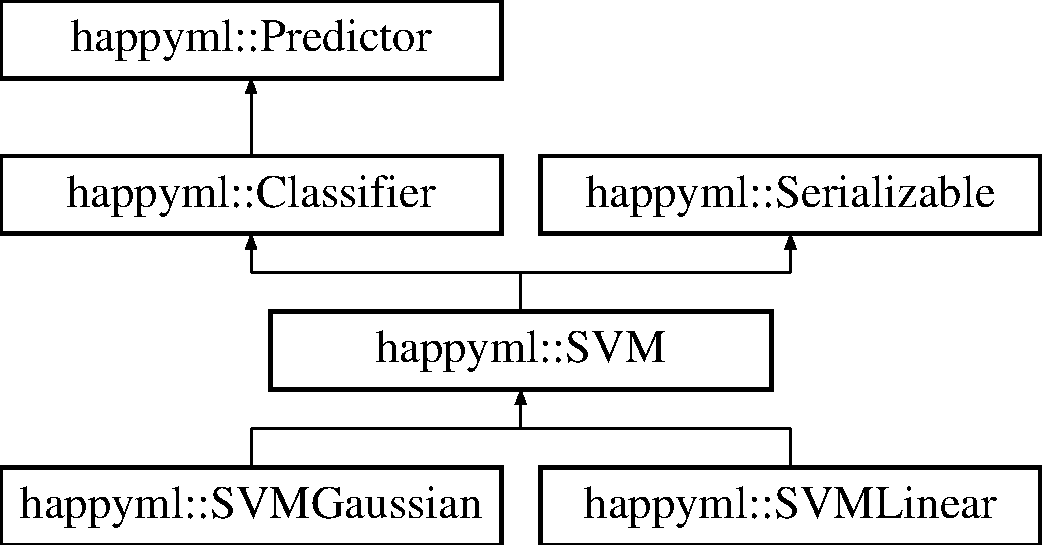
\includegraphics[height=4.000000cm]{classhappyml_1_1SVM}
\end{center}
\end{figure}
\subsection*{Public Member Functions}
\begin{DoxyCompactItemize}
\item 
\hyperlink{classhappyml_1_1SVM_a5507aedca56418aeb63abb0d18b1f133}{S\+VM} ()
\begin{DoxyCompactList}\small\item\em Creates a \hyperlink{classhappyml_1_1SVM}{S\+VM} without any support vector. \end{DoxyCompactList}\item 
double \hyperlink{classhappyml_1_1SVM_a9fce220acd57223df101009175dee53a}{get\+Bias} () const 
\begin{DoxyCompactList}\small\item\em Returns the bias term. \end{DoxyCompactList}\item 
int \hyperlink{classhappyml_1_1SVM_a4cc4569eb44c66c9a3a613042140319c}{get\+Number\+Support\+Vectors} () const 
\begin{DoxyCompactList}\small\item\em Returns the number of support vectors found. \end{DoxyCompactList}\item 
\hyperlink{classhappyml_1_1DataSet}{Data\+Set} \hyperlink{classhappyml_1_1SVM_a99e11b69c3b6583eb144ec1cd1f88000}{get\+Support\+Vectors} () const 
\begin{DoxyCompactList}\small\item\em Returns a dataset with the support vectors found. \end{DoxyCompactList}\item 
virtual double \hyperlink{classhappyml_1_1SVM_ac5d83933da1fdf70f1d20995136cfddd}{train} (const \hyperlink{classhappyml_1_1DataSet}{Data\+Set} \&data, double C=1, unsigned iter=5, double tolerance=0.\+001)
\begin{DoxyCompactList}\small\item\em Train the \hyperlink{classhappyml_1_1SVM}{S\+VM} using the given dataset and the given parameters. \end{DoxyCompactList}\item 
virtual double \hyperlink{classhappyml_1_1SVM_af29c307be8f6457806851f7274fc7c50}{predict} (const \hyperlink{namespacehappyml_a03602d1ec49393790b8a0449f40cd01f}{Input} \&x) const 
\begin{DoxyCompactList}\small\item\em Classifies an input vector. \end{DoxyCompactList}\item 
virtual double \hyperlink{classhappyml_1_1SVM_a940caf4789e40d6a2b237184765a16ea}{kernel} (vec x1, vec x2) const  =0
\begin{DoxyCompactList}\small\item\em Computes the similarity of the 2 vectors. \end{DoxyCompactList}\item 
void \hyperlink{classhappyml_1_1SVM_a180e169777af513b76cada99044ad3c3}{read} (istream \&stream)
\begin{DoxyCompactList}\small\item\em Read the object from an input stream. \end{DoxyCompactList}\item 
void \hyperlink{classhappyml_1_1SVM_a71cdc4e06322b9555dbcc118b45c4f73}{write} (ostream \&stream) const 
\begin{DoxyCompactList}\small\item\em Write the object to an output stream. \end{DoxyCompactList}\end{DoxyCompactItemize}
\subsection*{Protected Attributes}
\begin{DoxyCompactItemize}
\item 
\hyperlink{classhappyml_1_1DataSet}{Data\+Set} \hyperlink{classhappyml_1_1SVM_aa6fca9de47d16e821964229f660a8cdd}{sv}
\begin{DoxyCompactList}\small\item\em Support vectors. \end{DoxyCompactList}\item 
vec \hyperlink{classhappyml_1_1SVM_ab25126e39d5dc413f6acb22cf1d25cc8}{alphas}
\item 
double \hyperlink{classhappyml_1_1SVM_a84a61489971f2b76c78587aff4782fdc}{b}
\begin{DoxyCompactList}\small\item\em Bias term. \end{DoxyCompactList}\end{DoxyCompactItemize}


\subsection{Detailed Description}
Support vector machine with linear kernel. 

\subsection{Constructor \& Destructor Documentation}
\index{happyml\+::\+S\+VM@{happyml\+::\+S\+VM}!S\+VM@{S\+VM}}
\index{S\+VM@{S\+VM}!happyml\+::\+S\+VM@{happyml\+::\+S\+VM}}
\subsubsection[{\texorpdfstring{S\+V\+M()}{SVM()}}]{\setlength{\rightskip}{0pt plus 5cm}happyml\+::\+S\+V\+M\+::\+S\+VM (
\begin{DoxyParamCaption}
{}
\end{DoxyParamCaption}
)\hspace{0.3cm}{\ttfamily [inline]}}\hypertarget{classhappyml_1_1SVM_a5507aedca56418aeb63abb0d18b1f133}{}\label{classhappyml_1_1SVM_a5507aedca56418aeb63abb0d18b1f133}


Creates a \hyperlink{classhappyml_1_1SVM}{S\+VM} without any support vector. 

Needs to be trained. 

\subsection{Member Function Documentation}
\index{happyml\+::\+S\+VM@{happyml\+::\+S\+VM}!get\+Bias@{get\+Bias}}
\index{get\+Bias@{get\+Bias}!happyml\+::\+S\+VM@{happyml\+::\+S\+VM}}
\subsubsection[{\texorpdfstring{get\+Bias() const }{getBias() const }}]{\setlength{\rightskip}{0pt plus 5cm}double happyml\+::\+S\+V\+M\+::get\+Bias (
\begin{DoxyParamCaption}
{}
\end{DoxyParamCaption}
) const\hspace{0.3cm}{\ttfamily [inline]}}\hypertarget{classhappyml_1_1SVM_a9fce220acd57223df101009175dee53a}{}\label{classhappyml_1_1SVM_a9fce220acd57223df101009175dee53a}


Returns the bias term. 

It\textquotesingle{}s the first weight of the vector of weights.

\begin{DoxyReturn}{Returns}
Bias term. 
\end{DoxyReturn}
\index{happyml\+::\+S\+VM@{happyml\+::\+S\+VM}!get\+Number\+Support\+Vectors@{get\+Number\+Support\+Vectors}}
\index{get\+Number\+Support\+Vectors@{get\+Number\+Support\+Vectors}!happyml\+::\+S\+VM@{happyml\+::\+S\+VM}}
\subsubsection[{\texorpdfstring{get\+Number\+Support\+Vectors() const }{getNumberSupportVectors() const }}]{\setlength{\rightskip}{0pt plus 5cm}int happyml\+::\+S\+V\+M\+::get\+Number\+Support\+Vectors (
\begin{DoxyParamCaption}
{}
\end{DoxyParamCaption}
) const\hspace{0.3cm}{\ttfamily [inline]}}\hypertarget{classhappyml_1_1SVM_a4cc4569eb44c66c9a3a613042140319c}{}\label{classhappyml_1_1SVM_a4cc4569eb44c66c9a3a613042140319c}


Returns the number of support vectors found. 

\begin{DoxyReturn}{Returns}
Number of support vectors. 
\end{DoxyReturn}
\index{happyml\+::\+S\+VM@{happyml\+::\+S\+VM}!get\+Support\+Vectors@{get\+Support\+Vectors}}
\index{get\+Support\+Vectors@{get\+Support\+Vectors}!happyml\+::\+S\+VM@{happyml\+::\+S\+VM}}
\subsubsection[{\texorpdfstring{get\+Support\+Vectors() const }{getSupportVectors() const }}]{\setlength{\rightskip}{0pt plus 5cm}{\bf Data\+Set} happyml\+::\+S\+V\+M\+::get\+Support\+Vectors (
\begin{DoxyParamCaption}
{}
\end{DoxyParamCaption}
) const\hspace{0.3cm}{\ttfamily [inline]}}\hypertarget{classhappyml_1_1SVM_a99e11b69c3b6583eb144ec1cd1f88000}{}\label{classhappyml_1_1SVM_a99e11b69c3b6583eb144ec1cd1f88000}


Returns a dataset with the support vectors found. 

\begin{DoxyReturn}{Returns}
Dataset with the support vectors. 
\end{DoxyReturn}
\index{happyml\+::\+S\+VM@{happyml\+::\+S\+VM}!kernel@{kernel}}
\index{kernel@{kernel}!happyml\+::\+S\+VM@{happyml\+::\+S\+VM}}
\subsubsection[{\texorpdfstring{kernel(vec x1, vec x2) const  =0}{kernel(vec x1, vec x2) const  =0}}]{\setlength{\rightskip}{0pt plus 5cm}virtual double happyml\+::\+S\+V\+M\+::kernel (
\begin{DoxyParamCaption}
\item[{vec}]{x1, }
\item[{vec}]{x2}
\end{DoxyParamCaption}
) const\hspace{0.3cm}{\ttfamily [pure virtual]}}\hypertarget{classhappyml_1_1SVM_a940caf4789e40d6a2b237184765a16ea}{}\label{classhappyml_1_1SVM_a940caf4789e40d6a2b237184765a16ea}


Computes the similarity of the 2 vectors. 


\begin{DoxyParams}{Parameters}
{\em x1} & Vector 1. \\
\hline
{\em x2} & Vector 2. \\
\hline
\end{DoxyParams}


Implemented in \hyperlink{classhappyml_1_1SVMGaussian_a639e1a4002720ee7041db68be4254052}{happyml\+::\+S\+V\+M\+Gaussian}, and \hyperlink{classhappyml_1_1SVMLinear_ac7cb3d8280247f252b28d05d2fd10961}{happyml\+::\+S\+V\+M\+Linear}.

\index{happyml\+::\+S\+VM@{happyml\+::\+S\+VM}!predict@{predict}}
\index{predict@{predict}!happyml\+::\+S\+VM@{happyml\+::\+S\+VM}}
\subsubsection[{\texorpdfstring{predict(const Input \&x) const }{predict(const Input &x) const }}]{\setlength{\rightskip}{0pt plus 5cm}double happyml\+::\+S\+V\+M\+::predict (
\begin{DoxyParamCaption}
\item[{const {\bf Input} \&}]{x}
\end{DoxyParamCaption}
) const\hspace{0.3cm}{\ttfamily [virtual]}}\hypertarget{classhappyml_1_1SVM_af29c307be8f6457806851f7274fc7c50}{}\label{classhappyml_1_1SVM_af29c307be8f6457806851f7274fc7c50}


Classifies an input vector. 

\begin{DoxyReturn}{Returns}
$-1$ or $+1$. 
\end{DoxyReturn}


Implements \hyperlink{classhappyml_1_1Predictor_a07cf89d655e7642fd94c9b2a8fd0a04b}{happyml\+::\+Predictor}.



Reimplemented in \hyperlink{classhappyml_1_1SVMLinear_a7bf1f8e60104e34e0589b0b6cab1f447}{happyml\+::\+S\+V\+M\+Linear}.

\index{happyml\+::\+S\+VM@{happyml\+::\+S\+VM}!read@{read}}
\index{read@{read}!happyml\+::\+S\+VM@{happyml\+::\+S\+VM}}
\subsubsection[{\texorpdfstring{read(istream \&stream)}{read(istream &stream)}}]{\setlength{\rightskip}{0pt plus 5cm}void happyml\+::\+S\+V\+M\+::read (
\begin{DoxyParamCaption}
\item[{istream \&}]{stream}
\end{DoxyParamCaption}
)\hspace{0.3cm}{\ttfamily [virtual]}}\hypertarget{classhappyml_1_1SVM_a180e169777af513b76cada99044ad3c3}{}\label{classhappyml_1_1SVM_a180e169777af513b76cada99044ad3c3}


Read the object from an input stream. 


\begin{DoxyParams}{Parameters}
{\em stream} & Input stream. \\
\hline
\end{DoxyParams}


Implements \hyperlink{classhappyml_1_1Serializable_aef5c211d8e9c1c425b33c657824c2f0c}{happyml\+::\+Serializable}.



Reimplemented in \hyperlink{classhappyml_1_1SVMLinear_a4259c29ba1acd320703bf8c1ae8fd780}{happyml\+::\+S\+V\+M\+Linear}.

\index{happyml\+::\+S\+VM@{happyml\+::\+S\+VM}!train@{train}}
\index{train@{train}!happyml\+::\+S\+VM@{happyml\+::\+S\+VM}}
\subsubsection[{\texorpdfstring{train(const Data\+Set \&data, double C=1, unsigned iter=5, double tolerance=0.\+001)}{train(const DataSet &data, double C=1, unsigned iter=5, double tolerance=0.001)}}]{\setlength{\rightskip}{0pt plus 5cm}double happyml\+::\+S\+V\+M\+::train (
\begin{DoxyParamCaption}
\item[{const {\bf Data\+Set} \&}]{data, }
\item[{double}]{C = {\ttfamily 1}, }
\item[{unsigned}]{iter = {\ttfamily 5}, }
\item[{double}]{tolerance = {\ttfamily 0.001}}
\end{DoxyParamCaption}
)\hspace{0.3cm}{\ttfamily [virtual]}}\hypertarget{classhappyml_1_1SVM_ac5d83933da1fdf70f1d20995136cfddd}{}\label{classhappyml_1_1SVM_ac5d83933da1fdf70f1d20995136cfddd}


Train the \hyperlink{classhappyml_1_1SVM}{S\+VM} using the given dataset and the given parameters. 


\begin{DoxyParams}{Parameters}
{\em data} & Training set. \\
\hline
{\em C} & \hyperlink{classhappyml_1_1SVM}{S\+VM} regularization parameter. \\
\hline
{\em iter} & Maximun number of iterations that the S\+MO algorithm does all over the dataset. \\
\hline
{\em tolerance} & Tolerance that checks if a change in any alpha is significant to continue with other iteration.\\
\hline
\end{DoxyParams}
\begin{DoxyReturn}{Returns}
Returns the error of the \hyperlink{classhappyml_1_1SVM}{S\+VM}. 
\end{DoxyReturn}


Reimplemented in \hyperlink{classhappyml_1_1SVMLinear_a318e94752a99c25c000e9e176b8fa47e}{happyml\+::\+S\+V\+M\+Linear}.

\index{happyml\+::\+S\+VM@{happyml\+::\+S\+VM}!write@{write}}
\index{write@{write}!happyml\+::\+S\+VM@{happyml\+::\+S\+VM}}
\subsubsection[{\texorpdfstring{write(ostream \&stream) const }{write(ostream &stream) const }}]{\setlength{\rightskip}{0pt plus 5cm}void happyml\+::\+S\+V\+M\+::write (
\begin{DoxyParamCaption}
\item[{ostream \&}]{stream}
\end{DoxyParamCaption}
) const\hspace{0.3cm}{\ttfamily [virtual]}}\hypertarget{classhappyml_1_1SVM_a71cdc4e06322b9555dbcc118b45c4f73}{}\label{classhappyml_1_1SVM_a71cdc4e06322b9555dbcc118b45c4f73}


Write the object to an output stream. 


\begin{DoxyParams}{Parameters}
{\em stream} & Output stream. \\
\hline
\end{DoxyParams}


Implements \hyperlink{classhappyml_1_1Serializable_a2d503e4c2e39c5be8a33bcc8b691949f}{happyml\+::\+Serializable}.



\subsection{Member Data Documentation}
\index{happyml\+::\+S\+VM@{happyml\+::\+S\+VM}!alphas@{alphas}}
\index{alphas@{alphas}!happyml\+::\+S\+VM@{happyml\+::\+S\+VM}}
\subsubsection[{\texorpdfstring{alphas}{alphas}}]{\setlength{\rightskip}{0pt plus 5cm}vec happyml\+::\+S\+V\+M\+::alphas\hspace{0.3cm}{\ttfamily [protected]}}\hypertarget{classhappyml_1_1SVM_ab25126e39d5dc413f6acb22cf1d25cc8}{}\label{classhappyml_1_1SVM_ab25126e39d5dc413f6acb22cf1d25cc8}
\index{happyml\+::\+S\+VM@{happyml\+::\+S\+VM}!b@{b}}
\index{b@{b}!happyml\+::\+S\+VM@{happyml\+::\+S\+VM}}
\subsubsection[{\texorpdfstring{b}{b}}]{\setlength{\rightskip}{0pt plus 5cm}double happyml\+::\+S\+V\+M\+::b\hspace{0.3cm}{\ttfamily [protected]}}\hypertarget{classhappyml_1_1SVM_a84a61489971f2b76c78587aff4782fdc}{}\label{classhappyml_1_1SVM_a84a61489971f2b76c78587aff4782fdc}


Bias term. 

\index{happyml\+::\+S\+VM@{happyml\+::\+S\+VM}!sv@{sv}}
\index{sv@{sv}!happyml\+::\+S\+VM@{happyml\+::\+S\+VM}}
\subsubsection[{\texorpdfstring{sv}{sv}}]{\setlength{\rightskip}{0pt plus 5cm}{\bf Data\+Set} happyml\+::\+S\+V\+M\+::sv\hspace{0.3cm}{\ttfamily [protected]}}\hypertarget{classhappyml_1_1SVM_aa6fca9de47d16e821964229f660a8cdd}{}\label{classhappyml_1_1SVM_aa6fca9de47d16e821964229f660a8cdd}


Support vectors. 



The documentation for this class was generated from the following files\+:\begin{DoxyCompactItemize}
\item 
include/happyml/svm/\hyperlink{svm_8h}{svm.\+h}\item 
src/svm/\hyperlink{svm_8cpp}{svm.\+cpp}\end{DoxyCompactItemize}

\hypertarget{classhappyml_1_1SVMGaussian}{}\section{happyml\+:\+:S\+V\+M\+Gaussian Class Reference}
\label{classhappyml_1_1SVMGaussian}\index{happyml\+::\+S\+V\+M\+Gaussian@{happyml\+::\+S\+V\+M\+Gaussian}}


Support vector machine with linear kernel.  




{\ttfamily \#include $<$svm\+\_\+gaussian.\+h$>$}

Inheritance diagram for happyml\+:\+:S\+V\+M\+Gaussian\+:\begin{figure}[H]
\begin{center}
\leavevmode
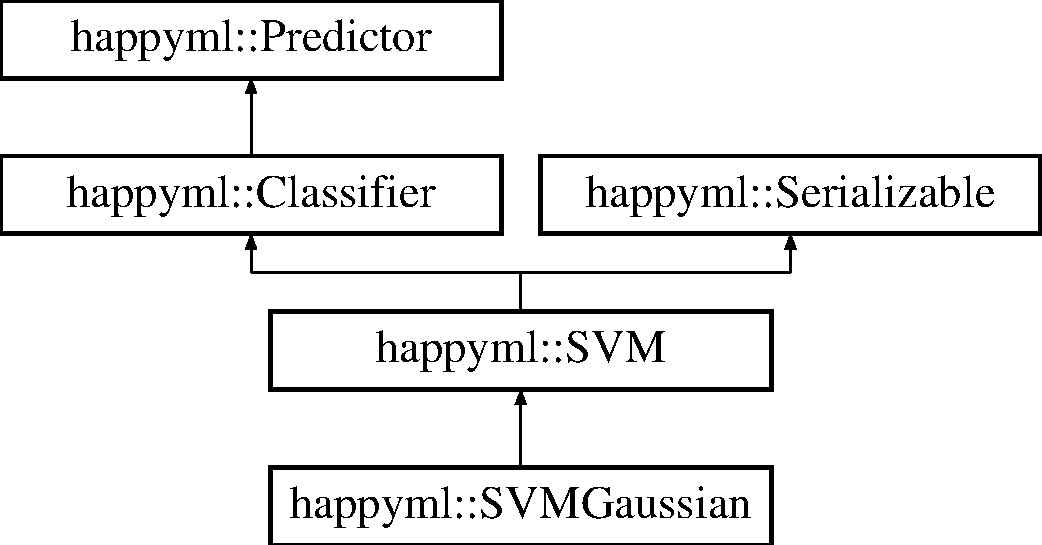
\includegraphics[height=4.000000cm]{classhappyml_1_1SVMGaussian}
\end{center}
\end{figure}
\subsection*{Public Member Functions}
\begin{DoxyCompactItemize}
\item 
\hyperlink{classhappyml_1_1SVMGaussian_ab1151f64a43cdb5e746d248f9945c894}{S\+V\+M\+Gaussian} (double s=1)
\begin{DoxyCompactList}\small\item\em Creates a guassian kernel \hyperlink{classhappyml_1_1SVM}{S\+VM} without any support vector. \end{DoxyCompactList}\item 
\hyperlink{classhappyml_1_1SVMGaussian_aa4a4e2329b1275c4b955fe9efd71deba}{$\sim$\+S\+V\+M\+Gaussian} ()
\item 
double \hyperlink{classhappyml_1_1SVMGaussian_a93a95615e16a223dbfe35897eff525ee}{get\+Sigma} () const 
\item 
void \hyperlink{classhappyml_1_1SVMGaussian_a08ceba8562b77aaf2eaca36d4cbaab05}{set\+Sigma} (double s)
\item 
double \hyperlink{classhappyml_1_1SVMGaussian_a639e1a4002720ee7041db68be4254052}{kernel} (vec x, vec z) const 
\begin{DoxyCompactList}\small\item\em Computes the similarity of the 2 vectors. \end{DoxyCompactList}\end{DoxyCompactItemize}
\subsection*{Protected Attributes}
\begin{DoxyCompactItemize}
\item 
double \hyperlink{classhappyml_1_1SVMGaussian_a18174d1f08ab7107c15e93812e194f09}{sigma}
\end{DoxyCompactItemize}


\subsection{Detailed Description}
Support vector machine with linear kernel. 

\subsection{Constructor \& Destructor Documentation}
\index{happyml\+::\+S\+V\+M\+Gaussian@{happyml\+::\+S\+V\+M\+Gaussian}!S\+V\+M\+Gaussian@{S\+V\+M\+Gaussian}}
\index{S\+V\+M\+Gaussian@{S\+V\+M\+Gaussian}!happyml\+::\+S\+V\+M\+Gaussian@{happyml\+::\+S\+V\+M\+Gaussian}}
\subsubsection[{\texorpdfstring{S\+V\+M\+Gaussian(double s=1)}{SVMGaussian(double s=1)}}]{\setlength{\rightskip}{0pt plus 5cm}happyml\+::\+S\+V\+M\+Gaussian\+::\+S\+V\+M\+Gaussian (
\begin{DoxyParamCaption}
\item[{double}]{s = {\ttfamily 1}}
\end{DoxyParamCaption}
)\hspace{0.3cm}{\ttfamily [inline]}}\hypertarget{classhappyml_1_1SVMGaussian_ab1151f64a43cdb5e746d248f9945c894}{}\label{classhappyml_1_1SVMGaussian_ab1151f64a43cdb5e746d248f9945c894}


Creates a guassian kernel \hyperlink{classhappyml_1_1SVM}{S\+VM} without any support vector. 

Needs to be trained.


\begin{DoxyParams}{Parameters}
{\em s} & Sigma gaussian kernel parameter. \\
\hline
\end{DoxyParams}
\index{happyml\+::\+S\+V\+M\+Gaussian@{happyml\+::\+S\+V\+M\+Gaussian}!````~S\+V\+M\+Gaussian@{$\sim$\+S\+V\+M\+Gaussian}}
\index{````~S\+V\+M\+Gaussian@{$\sim$\+S\+V\+M\+Gaussian}!happyml\+::\+S\+V\+M\+Gaussian@{happyml\+::\+S\+V\+M\+Gaussian}}
\subsubsection[{\texorpdfstring{$\sim$\+S\+V\+M\+Gaussian()}{~SVMGaussian()}}]{\setlength{\rightskip}{0pt plus 5cm}happyml\+::\+S\+V\+M\+Gaussian\+::$\sim$\+S\+V\+M\+Gaussian (
\begin{DoxyParamCaption}
{}
\end{DoxyParamCaption}
)\hspace{0.3cm}{\ttfamily [inline]}}\hypertarget{classhappyml_1_1SVMGaussian_aa4a4e2329b1275c4b955fe9efd71deba}{}\label{classhappyml_1_1SVMGaussian_aa4a4e2329b1275c4b955fe9efd71deba}


\subsection{Member Function Documentation}
\index{happyml\+::\+S\+V\+M\+Gaussian@{happyml\+::\+S\+V\+M\+Gaussian}!get\+Sigma@{get\+Sigma}}
\index{get\+Sigma@{get\+Sigma}!happyml\+::\+S\+V\+M\+Gaussian@{happyml\+::\+S\+V\+M\+Gaussian}}
\subsubsection[{\texorpdfstring{get\+Sigma() const }{getSigma() const }}]{\setlength{\rightskip}{0pt plus 5cm}double happyml\+::\+S\+V\+M\+Gaussian\+::get\+Sigma (
\begin{DoxyParamCaption}
{}
\end{DoxyParamCaption}
) const\hspace{0.3cm}{\ttfamily [inline]}}\hypertarget{classhappyml_1_1SVMGaussian_a93a95615e16a223dbfe35897eff525ee}{}\label{classhappyml_1_1SVMGaussian_a93a95615e16a223dbfe35897eff525ee}
\index{happyml\+::\+S\+V\+M\+Gaussian@{happyml\+::\+S\+V\+M\+Gaussian}!kernel@{kernel}}
\index{kernel@{kernel}!happyml\+::\+S\+V\+M\+Gaussian@{happyml\+::\+S\+V\+M\+Gaussian}}
\subsubsection[{\texorpdfstring{kernel(vec x, vec z) const }{kernel(vec x, vec z) const }}]{\setlength{\rightskip}{0pt plus 5cm}double happyml\+::\+S\+V\+M\+Gaussian\+::kernel (
\begin{DoxyParamCaption}
\item[{vec}]{x1, }
\item[{vec}]{x2}
\end{DoxyParamCaption}
) const\hspace{0.3cm}{\ttfamily [virtual]}}\hypertarget{classhappyml_1_1SVMGaussian_a639e1a4002720ee7041db68be4254052}{}\label{classhappyml_1_1SVMGaussian_a639e1a4002720ee7041db68be4254052}


Computes the similarity of the 2 vectors. 


\begin{DoxyParams}{Parameters}
{\em x1} & Vector 1. \\
\hline
{\em x2} & Vector 2. \\
\hline
\end{DoxyParams}


Implements \hyperlink{classhappyml_1_1SVM_a940caf4789e40d6a2b237184765a16ea}{happyml\+::\+S\+VM}.

\index{happyml\+::\+S\+V\+M\+Gaussian@{happyml\+::\+S\+V\+M\+Gaussian}!set\+Sigma@{set\+Sigma}}
\index{set\+Sigma@{set\+Sigma}!happyml\+::\+S\+V\+M\+Gaussian@{happyml\+::\+S\+V\+M\+Gaussian}}
\subsubsection[{\texorpdfstring{set\+Sigma(double s)}{setSigma(double s)}}]{\setlength{\rightskip}{0pt plus 5cm}void happyml\+::\+S\+V\+M\+Gaussian\+::set\+Sigma (
\begin{DoxyParamCaption}
\item[{double}]{s}
\end{DoxyParamCaption}
)\hspace{0.3cm}{\ttfamily [inline]}}\hypertarget{classhappyml_1_1SVMGaussian_a08ceba8562b77aaf2eaca36d4cbaab05}{}\label{classhappyml_1_1SVMGaussian_a08ceba8562b77aaf2eaca36d4cbaab05}


\subsection{Member Data Documentation}
\index{happyml\+::\+S\+V\+M\+Gaussian@{happyml\+::\+S\+V\+M\+Gaussian}!sigma@{sigma}}
\index{sigma@{sigma}!happyml\+::\+S\+V\+M\+Gaussian@{happyml\+::\+S\+V\+M\+Gaussian}}
\subsubsection[{\texorpdfstring{sigma}{sigma}}]{\setlength{\rightskip}{0pt plus 5cm}double happyml\+::\+S\+V\+M\+Gaussian\+::sigma\hspace{0.3cm}{\ttfamily [protected]}}\hypertarget{classhappyml_1_1SVMGaussian_a18174d1f08ab7107c15e93812e194f09}{}\label{classhappyml_1_1SVMGaussian_a18174d1f08ab7107c15e93812e194f09}


The documentation for this class was generated from the following files\+:\begin{DoxyCompactItemize}
\item 
include/happyml/svm/\hyperlink{svm__gaussian_8h}{svm\+\_\+gaussian.\+h}\item 
src/svm/\hyperlink{svm__gaussian_8cpp}{svm\+\_\+gaussian.\+cpp}\end{DoxyCompactItemize}

\hypertarget{classhappyml_1_1SVMLinear}{}\section{happyml\+:\+:S\+V\+M\+Linear Class Reference}
\label{classhappyml_1_1SVMLinear}\index{happyml\+::\+S\+V\+M\+Linear@{happyml\+::\+S\+V\+M\+Linear}}


Support vector machine with linear kernel.  




{\ttfamily \#include $<$svm\+\_\+linear.\+h$>$}

Inheritance diagram for happyml\+:\+:S\+V\+M\+Linear\+:\begin{figure}[H]
\begin{center}
\leavevmode
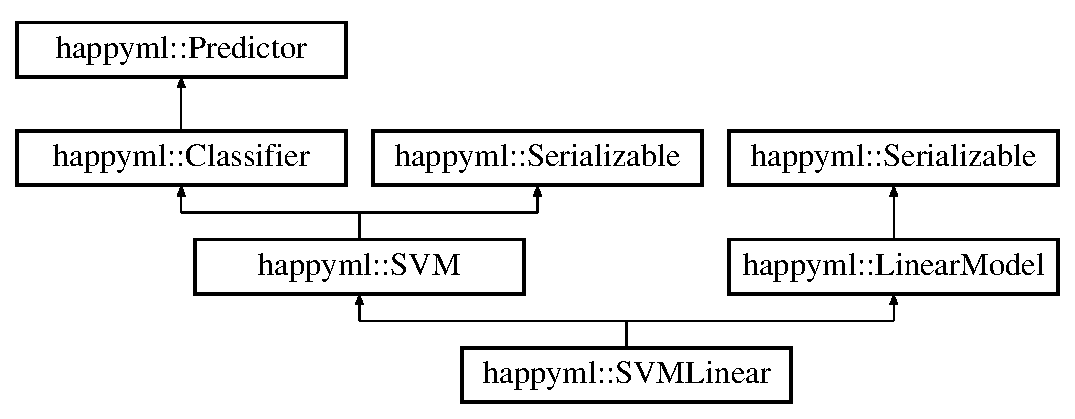
\includegraphics[height=4.000000cm]{classhappyml_1_1SVMLinear}
\end{center}
\end{figure}
\subsection*{Public Member Functions}
\begin{DoxyCompactItemize}
\item 
\hyperlink{classhappyml_1_1SVMLinear_a02451aa99f38b386702d68014a6b924f}{S\+V\+M\+Linear} ()
\begin{DoxyCompactList}\small\item\em Creates a linear kernel \hyperlink{classhappyml_1_1SVM}{S\+VM} without any support vector. \end{DoxyCompactList}\item 
\hyperlink{classhappyml_1_1SVMLinear_a8f204fd440955dca167c113df0dbaf73}{$\sim$\+S\+V\+M\+Linear} ()
\item 
double \hyperlink{classhappyml_1_1SVMLinear_a318e94752a99c25c000e9e176b8fa47e}{train} (const \hyperlink{classhappyml_1_1DataSet}{Data\+Set} \&data, double C=1, unsigned iter=5, double tolerance=0.\+001)
\begin{DoxyCompactList}\small\item\em Train the \hyperlink{classhappyml_1_1SVM}{S\+VM} using the given dataset and the given parameters. \end{DoxyCompactList}\item 
double \hyperlink{classhappyml_1_1SVMLinear_ac7cb3d8280247f252b28d05d2fd10961}{kernel} (vec x, vec z) const 
\begin{DoxyCompactList}\small\item\em Computes the similarity of the 2 vectors. \end{DoxyCompactList}\item 
double \hyperlink{classhappyml_1_1SVMLinear_a7bf1f8e60104e34e0589b0b6cab1f447}{predict} (const \hyperlink{namespacehappyml_a03602d1ec49393790b8a0449f40cd01f}{Input} \&input) const 
\begin{DoxyCompactList}\small\item\em Classifies an input vector. \end{DoxyCompactList}\item 
void \hyperlink{classhappyml_1_1SVMLinear_a4259c29ba1acd320703bf8c1ae8fd780}{read} (istream \&stream)
\begin{DoxyCompactList}\small\item\em Read the weight vector from the text stream. \end{DoxyCompactList}\end{DoxyCompactItemize}
\subsection*{Additional Inherited Members}


\subsection{Detailed Description}
Support vector machine with linear kernel. 

\subsection{Constructor \& Destructor Documentation}
\index{happyml\+::\+S\+V\+M\+Linear@{happyml\+::\+S\+V\+M\+Linear}!S\+V\+M\+Linear@{S\+V\+M\+Linear}}
\index{S\+V\+M\+Linear@{S\+V\+M\+Linear}!happyml\+::\+S\+V\+M\+Linear@{happyml\+::\+S\+V\+M\+Linear}}
\subsubsection[{\texorpdfstring{S\+V\+M\+Linear()}{SVMLinear()}}]{\setlength{\rightskip}{0pt plus 5cm}happyml\+::\+S\+V\+M\+Linear\+::\+S\+V\+M\+Linear (
\begin{DoxyParamCaption}
{}
\end{DoxyParamCaption}
)\hspace{0.3cm}{\ttfamily [inline]}}\hypertarget{classhappyml_1_1SVMLinear_a02451aa99f38b386702d68014a6b924f}{}\label{classhappyml_1_1SVMLinear_a02451aa99f38b386702d68014a6b924f}


Creates a linear kernel \hyperlink{classhappyml_1_1SVM}{S\+VM} without any support vector. 

Needs to be trained. \index{happyml\+::\+S\+V\+M\+Linear@{happyml\+::\+S\+V\+M\+Linear}!````~S\+V\+M\+Linear@{$\sim$\+S\+V\+M\+Linear}}
\index{````~S\+V\+M\+Linear@{$\sim$\+S\+V\+M\+Linear}!happyml\+::\+S\+V\+M\+Linear@{happyml\+::\+S\+V\+M\+Linear}}
\subsubsection[{\texorpdfstring{$\sim$\+S\+V\+M\+Linear()}{~SVMLinear()}}]{\setlength{\rightskip}{0pt plus 5cm}happyml\+::\+S\+V\+M\+Linear\+::$\sim$\+S\+V\+M\+Linear (
\begin{DoxyParamCaption}
{}
\end{DoxyParamCaption}
)\hspace{0.3cm}{\ttfamily [inline]}}\hypertarget{classhappyml_1_1SVMLinear_a8f204fd440955dca167c113df0dbaf73}{}\label{classhappyml_1_1SVMLinear_a8f204fd440955dca167c113df0dbaf73}


\subsection{Member Function Documentation}
\index{happyml\+::\+S\+V\+M\+Linear@{happyml\+::\+S\+V\+M\+Linear}!kernel@{kernel}}
\index{kernel@{kernel}!happyml\+::\+S\+V\+M\+Linear@{happyml\+::\+S\+V\+M\+Linear}}
\subsubsection[{\texorpdfstring{kernel(vec x, vec z) const }{kernel(vec x, vec z) const }}]{\setlength{\rightskip}{0pt plus 5cm}double happyml\+::\+S\+V\+M\+Linear\+::kernel (
\begin{DoxyParamCaption}
\item[{vec}]{x1, }
\item[{vec}]{x2}
\end{DoxyParamCaption}
) const\hspace{0.3cm}{\ttfamily [virtual]}}\hypertarget{classhappyml_1_1SVMLinear_ac7cb3d8280247f252b28d05d2fd10961}{}\label{classhappyml_1_1SVMLinear_ac7cb3d8280247f252b28d05d2fd10961}


Computes the similarity of the 2 vectors. 


\begin{DoxyParams}{Parameters}
{\em x1} & Vector 1. \\
\hline
{\em x2} & Vector 2. \\
\hline
\end{DoxyParams}


Implements \hyperlink{classhappyml_1_1SVM_a940caf4789e40d6a2b237184765a16ea}{happyml\+::\+S\+VM}.

\index{happyml\+::\+S\+V\+M\+Linear@{happyml\+::\+S\+V\+M\+Linear}!predict@{predict}}
\index{predict@{predict}!happyml\+::\+S\+V\+M\+Linear@{happyml\+::\+S\+V\+M\+Linear}}
\subsubsection[{\texorpdfstring{predict(const Input \&input) const }{predict(const Input &input) const }}]{\setlength{\rightskip}{0pt plus 5cm}double happyml\+::\+S\+V\+M\+Linear\+::predict (
\begin{DoxyParamCaption}
\item[{const {\bf Input} \&}]{x}
\end{DoxyParamCaption}
) const\hspace{0.3cm}{\ttfamily [virtual]}}\hypertarget{classhappyml_1_1SVMLinear_a7bf1f8e60104e34e0589b0b6cab1f447}{}\label{classhappyml_1_1SVMLinear_a7bf1f8e60104e34e0589b0b6cab1f447}


Classifies an input vector. 

\begin{DoxyReturn}{Returns}
$-1$ or $+1$. 
\end{DoxyReturn}


Reimplemented from \hyperlink{classhappyml_1_1SVM_af29c307be8f6457806851f7274fc7c50}{happyml\+::\+S\+VM}.

\index{happyml\+::\+S\+V\+M\+Linear@{happyml\+::\+S\+V\+M\+Linear}!read@{read}}
\index{read@{read}!happyml\+::\+S\+V\+M\+Linear@{happyml\+::\+S\+V\+M\+Linear}}
\subsubsection[{\texorpdfstring{read(istream \&stream)}{read(istream &stream)}}]{\setlength{\rightskip}{0pt plus 5cm}void happyml\+::\+S\+V\+M\+Linear\+::read (
\begin{DoxyParamCaption}
\item[{istream \&}]{stream}
\end{DoxyParamCaption}
)\hspace{0.3cm}{\ttfamily [virtual]}}\hypertarget{classhappyml_1_1SVMLinear_a4259c29ba1acd320703bf8c1ae8fd780}{}\label{classhappyml_1_1SVMLinear_a4259c29ba1acd320703bf8c1ae8fd780}


Read the weight vector from the text stream. 

Format of the stream\+: $\\ w_{0}\\ w_{1}\\ \ \ \vdots\\ w_{d} $


\begin{DoxyParams}{Parameters}
{\em stream} & Input stream. \\
\hline
\end{DoxyParams}


Reimplemented from \hyperlink{classhappyml_1_1LinearModel_abdc75a19c7234d8bc13b4dd7ad621c9e}{happyml\+::\+Linear\+Model}.

\index{happyml\+::\+S\+V\+M\+Linear@{happyml\+::\+S\+V\+M\+Linear}!train@{train}}
\index{train@{train}!happyml\+::\+S\+V\+M\+Linear@{happyml\+::\+S\+V\+M\+Linear}}
\subsubsection[{\texorpdfstring{train(const Data\+Set \&data, double C=1, unsigned iter=5, double tolerance=0.\+001)}{train(const DataSet &data, double C=1, unsigned iter=5, double tolerance=0.001)}}]{\setlength{\rightskip}{0pt plus 5cm}double happyml\+::\+S\+V\+M\+Linear\+::train (
\begin{DoxyParamCaption}
\item[{const {\bf Data\+Set} \&}]{data, }
\item[{double}]{C = {\ttfamily 1}, }
\item[{unsigned}]{iter = {\ttfamily 5}, }
\item[{double}]{tolerance = {\ttfamily 0.001}}
\end{DoxyParamCaption}
)\hspace{0.3cm}{\ttfamily [virtual]}}\hypertarget{classhappyml_1_1SVMLinear_a318e94752a99c25c000e9e176b8fa47e}{}\label{classhappyml_1_1SVMLinear_a318e94752a99c25c000e9e176b8fa47e}


Train the \hyperlink{classhappyml_1_1SVM}{S\+VM} using the given dataset and the given parameters. 


\begin{DoxyParams}{Parameters}
{\em data} & Training set. \\
\hline
{\em C} & \hyperlink{classhappyml_1_1SVM}{S\+VM} regularization parameter. \\
\hline
{\em iter} & Maximun number of iterations that the S\+MO algorithm does all over the dataset. \\
\hline
{\em tolerance} & Tolerance that checks if a change in any alpha is significant to continue with other iteration.\\
\hline
\end{DoxyParams}
\begin{DoxyReturn}{Returns}
Returns the error of the \hyperlink{classhappyml_1_1SVM}{S\+VM}. 
\end{DoxyReturn}


Reimplemented from \hyperlink{classhappyml_1_1SVM_ac5d83933da1fdf70f1d20995136cfddd}{happyml\+::\+S\+VM}.



The documentation for this class was generated from the following files\+:\begin{DoxyCompactItemize}
\item 
include/happyml/svm/\hyperlink{svm__linear_8h}{svm\+\_\+linear.\+h}\item 
src/svm/\hyperlink{svm__linear_8cpp}{svm\+\_\+linear.\+cpp}\end{DoxyCompactItemize}

\hypertarget{classhappyml_1_1TrainingProcess}{}\section{happyml\+:\+:Training\+Process Class Reference}
\label{classhappyml_1_1TrainingProcess}\index{happyml\+::\+Training\+Process@{happyml\+::\+Training\+Process}}


{\ttfamily \#include $<$k\+\_\+fold\+\_\+cross\+\_\+validation.\+h$>$}

\subsection*{Public Member Functions}
\begin{DoxyCompactItemize}
\item 
virtual void \hyperlink{classhappyml_1_1TrainingProcess_af203071393b6159f12d115fa14747d37}{run} (const \hyperlink{classhappyml_1_1DataSet}{Data\+Set} \&training, const \hyperlink{classhappyml_1_1DataSet}{Data\+Set} \&cv)=0
\end{DoxyCompactItemize}


\subsection{Member Function Documentation}
\index{happyml\+::\+Training\+Process@{happyml\+::\+Training\+Process}!run@{run}}
\index{run@{run}!happyml\+::\+Training\+Process@{happyml\+::\+Training\+Process}}
\subsubsection[{\texorpdfstring{run(const Data\+Set \&training, const Data\+Set \&cv)=0}{run(const DataSet &training, const DataSet &cv)=0}}]{\setlength{\rightskip}{0pt plus 5cm}virtual void happyml\+::\+Training\+Process\+::run (
\begin{DoxyParamCaption}
\item[{const {\bf Data\+Set} \&}]{training, }
\item[{const {\bf Data\+Set} \&}]{cv}
\end{DoxyParamCaption}
)\hspace{0.3cm}{\ttfamily [pure virtual]}}\hypertarget{classhappyml_1_1TrainingProcess_af203071393b6159f12d115fa14747d37}{}\label{classhappyml_1_1TrainingProcess_af203071393b6159f12d115fa14747d37}


The documentation for this class was generated from the following file\+:\begin{DoxyCompactItemize}
\item 
include/happyml/\hyperlink{k__fold__cross__validation_8h}{k\+\_\+fold\+\_\+cross\+\_\+validation.\+h}\end{DoxyCompactItemize}

\hypertarget{classhappyml_1_1Transformer}{}\section{happyml\+:\+:Transformer Class Reference}
\label{classhappyml_1_1Transformer}\index{happyml\+::\+Transformer@{happyml\+::\+Transformer}}


Class that applies linear and non-\/linear transformations to an input or to a whole dataset.  




{\ttfamily \#include $<$transformer.\+h$>$}

Inheritance diagram for happyml\+:\+:Transformer\+:\begin{figure}[H]
\begin{center}
\leavevmode
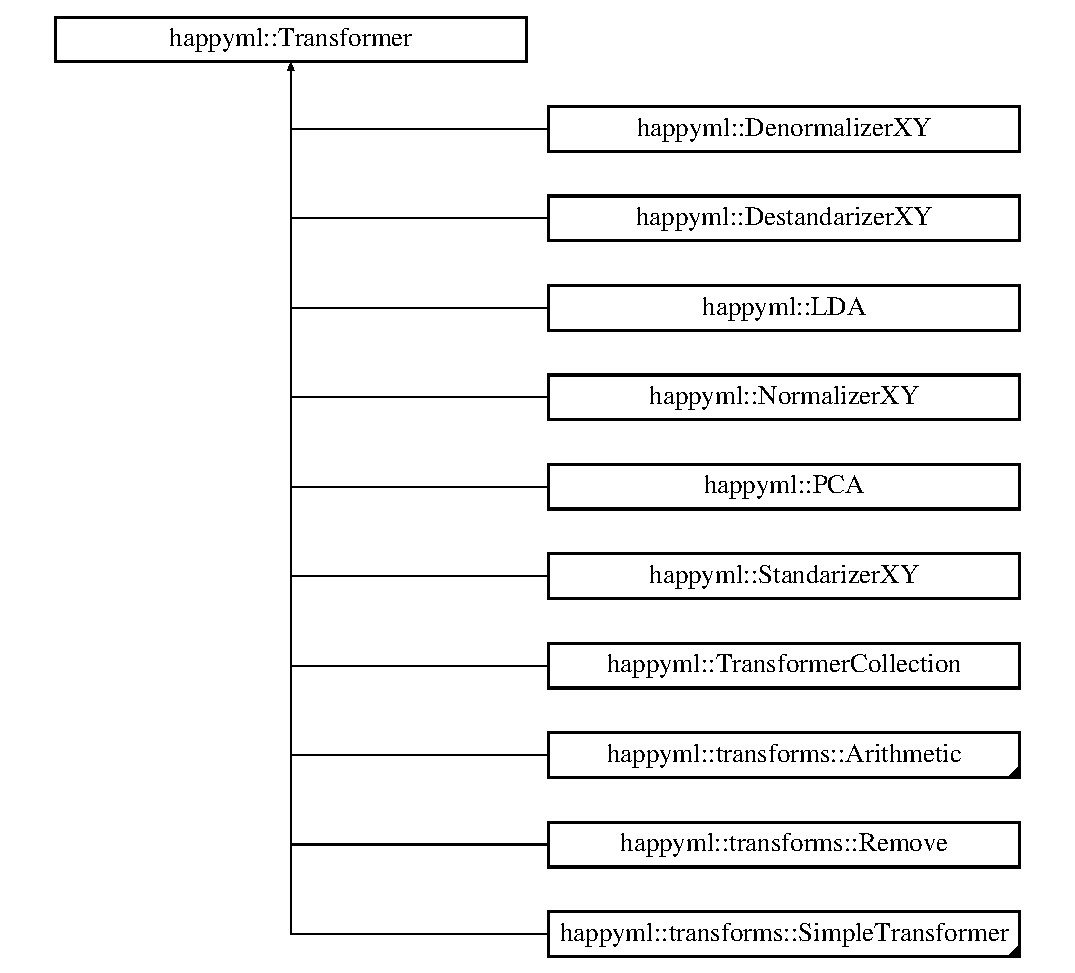
\includegraphics[height=11.000000cm]{classhappyml_1_1Transformer}
\end{center}
\end{figure}
\subsection*{Public Member Functions}
\begin{DoxyCompactItemize}
\item 
\hyperlink{classhappyml_1_1Transformer_a10074d87318ab9db84cc477b5ec66967}{Transformer} ()
\item 
\hyperlink{classhappyml_1_1Transformer_a3c6fb3c19e318ee24c8d233c94e5eb13}{$\sim$\+Transformer} ()
\item 
virtual void \hyperlink{classhappyml_1_1Transformer_a169a2a8434124c1dd8e671bca2cfa71d}{apply} (\hyperlink{classhappyml_1_1DataSet}{Data\+Set} \&dataset) const 
\begin{DoxyCompactList}\small\item\em Applies all the transformations at the given dataset. \end{DoxyCompactList}\item 
virtual \hyperlink{namespacehappyml_a03602d1ec49393790b8a0449f40cd01f}{Input} \hyperlink{classhappyml_1_1Transformer_a3e0eb67990c90c461466307fdefab45c}{apply} (const \hyperlink{namespacehappyml_a03602d1ec49393790b8a0449f40cd01f}{Input} \&input) const 
\begin{DoxyCompactList}\small\item\em Applies all the transformations at the given input. \end{DoxyCompactList}\end{DoxyCompactItemize}


\subsection{Detailed Description}
Class that applies linear and non-\/linear transformations to an input or to a whole dataset. 

\subsection{Constructor \& Destructor Documentation}
\index{happyml\+::\+Transformer@{happyml\+::\+Transformer}!Transformer@{Transformer}}
\index{Transformer@{Transformer}!happyml\+::\+Transformer@{happyml\+::\+Transformer}}
\subsubsection[{\texorpdfstring{Transformer()}{Transformer()}}]{\setlength{\rightskip}{0pt plus 5cm}happyml\+::\+Transformer\+::\+Transformer (
\begin{DoxyParamCaption}
{}
\end{DoxyParamCaption}
)\hspace{0.3cm}{\ttfamily [inline]}}\hypertarget{classhappyml_1_1Transformer_a10074d87318ab9db84cc477b5ec66967}{}\label{classhappyml_1_1Transformer_a10074d87318ab9db84cc477b5ec66967}
\index{happyml\+::\+Transformer@{happyml\+::\+Transformer}!````~Transformer@{$\sim$\+Transformer}}
\index{````~Transformer@{$\sim$\+Transformer}!happyml\+::\+Transformer@{happyml\+::\+Transformer}}
\subsubsection[{\texorpdfstring{$\sim$\+Transformer()}{~Transformer()}}]{\setlength{\rightskip}{0pt plus 5cm}happyml\+::\+Transformer\+::$\sim$\+Transformer (
\begin{DoxyParamCaption}
{}
\end{DoxyParamCaption}
)\hspace{0.3cm}{\ttfamily [inline]}}\hypertarget{classhappyml_1_1Transformer_a3c6fb3c19e318ee24c8d233c94e5eb13}{}\label{classhappyml_1_1Transformer_a3c6fb3c19e318ee24c8d233c94e5eb13}


\subsection{Member Function Documentation}
\index{happyml\+::\+Transformer@{happyml\+::\+Transformer}!apply@{apply}}
\index{apply@{apply}!happyml\+::\+Transformer@{happyml\+::\+Transformer}}
\subsubsection[{\texorpdfstring{apply(\+Data\+Set \&dataset) const }{apply(DataSet &dataset) const }}]{\setlength{\rightskip}{0pt plus 5cm}virtual void happyml\+::\+Transformer\+::apply (
\begin{DoxyParamCaption}
\item[{{\bf Data\+Set} \&}]{dataset}
\end{DoxyParamCaption}
) const\hspace{0.3cm}{\ttfamily [inline]}, {\ttfamily [virtual]}}\hypertarget{classhappyml_1_1Transformer_a169a2a8434124c1dd8e671bca2cfa71d}{}\label{classhappyml_1_1Transformer_a169a2a8434124c1dd8e671bca2cfa71d}


Applies all the transformations at the given dataset. 


\begin{DoxyParams}{Parameters}
{\em dataset} & Dataset to transform. \\
\hline
\end{DoxyParams}


Reimplemented in \hyperlink{classhappyml_1_1transforms_1_1SimpleTransformer_a7bb7863c5f6b2e0a36eac155b1f25cdf}{happyml\+::transforms\+::\+Simple\+Transformer}, \hyperlink{classhappyml_1_1DenormalizerXY_a724e14e520004b2d66611c0e152a9d3b}{happyml\+::\+Denormalizer\+XY}, \hyperlink{classhappyml_1_1DestandarizerXY_a84c63216d9a78bc61647550381fed0a6}{happyml\+::\+Destandarizer\+XY}, \hyperlink{classhappyml_1_1transforms_1_1Remove_a901c9a5c55f4b360233b8ba7e46fc198}{happyml\+::transforms\+::\+Remove}, \hyperlink{classhappyml_1_1transforms_1_1Arithmetic_aafe6e2ef231e5515f2068b8340aac93a}{happyml\+::transforms\+::\+Arithmetic}, \hyperlink{classhappyml_1_1NormalizerXY_ac843088ef9e2189ed719f4556ba111e2}{happyml\+::\+Normalizer\+XY}, \hyperlink{classhappyml_1_1StandarizerXY_af2979980c88b3c5c4d670d2148c148e8}{happyml\+::\+Standarizer\+XY}, \hyperlink{classhappyml_1_1PCA_a298495b3f3cf0ed3b623392a6f89b719}{happyml\+::\+P\+CA}, \hyperlink{classhappyml_1_1TransformerCollection_a20fd27b57eb8fa4546e3664ea33283f1}{happyml\+::\+Transformer\+Collection}, and \hyperlink{classhappyml_1_1LDA_a642ebe3b7cfcddaa5b21cd93ed1cf082}{happyml\+::\+L\+DA}.

\index{happyml\+::\+Transformer@{happyml\+::\+Transformer}!apply@{apply}}
\index{apply@{apply}!happyml\+::\+Transformer@{happyml\+::\+Transformer}}
\subsubsection[{\texorpdfstring{apply(const Input \&input) const }{apply(const Input &input) const }}]{\setlength{\rightskip}{0pt plus 5cm}virtual {\bf Input} happyml\+::\+Transformer\+::apply (
\begin{DoxyParamCaption}
\item[{const {\bf Input} \&}]{input}
\end{DoxyParamCaption}
) const\hspace{0.3cm}{\ttfamily [inline]}, {\ttfamily [virtual]}}\hypertarget{classhappyml_1_1Transformer_a3e0eb67990c90c461466307fdefab45c}{}\label{classhappyml_1_1Transformer_a3e0eb67990c90c461466307fdefab45c}


Applies all the transformations at the given input. 


\begin{DoxyParams}{Parameters}
{\em input} & Input to transform.\\
\hline
\end{DoxyParams}
\begin{DoxyReturn}{Returns}
A transformated version of the input. 
\end{DoxyReturn}


Reimplemented in \hyperlink{classhappyml_1_1DenormalizerXY_a22e45e0e3595ede802dca4c4cf772a73}{happyml\+::\+Denormalizer\+XY}, \hyperlink{classhappyml_1_1DestandarizerXY_a21481d414441642b50b04d43f6c55ac0}{happyml\+::\+Destandarizer\+XY}, \hyperlink{classhappyml_1_1transforms_1_1Remove_a249eec291d4c15b4e8e044c38a994770}{happyml\+::transforms\+::\+Remove}, \hyperlink{classhappyml_1_1transforms_1_1Arithmetic_ac32e38e089435dc407bc9b7a338bc845}{happyml\+::transforms\+::\+Arithmetic}, \hyperlink{classhappyml_1_1NormalizerXY_a0f10be1b98dfc3125990310ee649ee8e}{happyml\+::\+Normalizer\+XY}, \hyperlink{classhappyml_1_1StandarizerXY_a800a8953dbf96c26edca660680ce791f}{happyml\+::\+Standarizer\+XY}, \hyperlink{classhappyml_1_1TransformerCollection_a36511b731522cda1cadbe3fa4299f6bf}{happyml\+::\+Transformer\+Collection}, \hyperlink{classhappyml_1_1PCA_a2a630892c653832287bb3df4ab002d51}{happyml\+::\+P\+CA}, and \hyperlink{classhappyml_1_1LDA_a2b98a4675abdb0985347491224136b5c}{happyml\+::\+L\+DA}.



The documentation for this class was generated from the following file\+:\begin{DoxyCompactItemize}
\item 
include/happyml/transformers/\hyperlink{transformer_8h}{transformer.\+h}\end{DoxyCompactItemize}

\hypertarget{classhappyml_1_1TransformerCollection}{}\section{happyml\+:\+:Transformer\+Collection Class Reference}
\label{classhappyml_1_1TransformerCollection}\index{happyml\+::\+Transformer\+Collection@{happyml\+::\+Transformer\+Collection}}


\hyperlink{classhappyml_1_1Transformer}{Transformer} that applies a collection of transformers to a given input or dataset.  




{\ttfamily \#include $<$transformer.\+h$>$}

Inheritance diagram for happyml\+:\+:Transformer\+Collection\+:\begin{figure}[H]
\begin{center}
\leavevmode
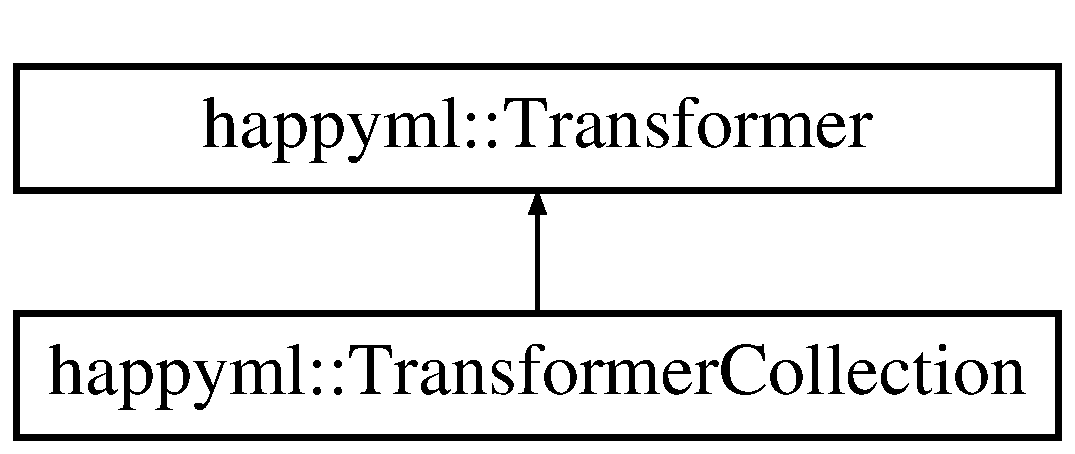
\includegraphics[height=2.000000cm]{classhappyml_1_1TransformerCollection}
\end{center}
\end{figure}
\subsection*{Public Member Functions}
\begin{DoxyCompactItemize}
\item 
\hyperlink{classhappyml_1_1TransformerCollection_ab994ad8673d0d966d5eb40057312d5d4}{Transformer\+Collection} ()
\item 
\hyperlink{classhappyml_1_1TransformerCollection_abde2c02d4e68015d0dd86c15fc3f8dd3}{$\sim$\+Transformer\+Collection} ()
\item 
void \hyperlink{classhappyml_1_1TransformerCollection_a20fd27b57eb8fa4546e3664ea33283f1}{apply} (\hyperlink{classhappyml_1_1DataSet}{Data\+Set} \&dataset) const 
\begin{DoxyCompactList}\small\item\em Applies all the transformers in the order that were added to the collection. \end{DoxyCompactList}\item 
\hyperlink{namespacehappyml_a03602d1ec49393790b8a0449f40cd01f}{Input} \hyperlink{classhappyml_1_1TransformerCollection_a36511b731522cda1cadbe3fa4299f6bf}{apply} (const \hyperlink{namespacehappyml_a03602d1ec49393790b8a0449f40cd01f}{Input} \&input) const 
\begin{DoxyCompactList}\small\item\em Applies all the transformers in the order that were added to the collection. \end{DoxyCompactList}\item 
void \hyperlink{classhappyml_1_1TransformerCollection_a443ff8b53921d921765b0396d17037e4}{add} (const \hyperlink{classhappyml_1_1Transformer}{Transformer} $\ast$t)
\begin{DoxyCompactList}\small\item\em Adds a new \hyperlink{classhappyml_1_1Transformer}{Transformer} to the collection that will be executed when the apply\textquotesingle{}s methods it will be called. \end{DoxyCompactList}\end{DoxyCompactItemize}
\subsection*{Protected Attributes}
\begin{DoxyCompactItemize}
\item 
vector$<$ const \hyperlink{classhappyml_1_1Transformer}{Transformer} $\ast$ $>$ \hyperlink{classhappyml_1_1TransformerCollection_a90c2b12199efa361dedf28f01a72d9ff}{transformers}
\end{DoxyCompactItemize}


\subsection{Detailed Description}
\hyperlink{classhappyml_1_1Transformer}{Transformer} that applies a collection of transformers to a given input or dataset. 

\subsection{Constructor \& Destructor Documentation}
\index{happyml\+::\+Transformer\+Collection@{happyml\+::\+Transformer\+Collection}!Transformer\+Collection@{Transformer\+Collection}}
\index{Transformer\+Collection@{Transformer\+Collection}!happyml\+::\+Transformer\+Collection@{happyml\+::\+Transformer\+Collection}}
\subsubsection[{\texorpdfstring{Transformer\+Collection()}{TransformerCollection()}}]{\setlength{\rightskip}{0pt plus 5cm}happyml\+::\+Transformer\+Collection\+::\+Transformer\+Collection (
\begin{DoxyParamCaption}
{}
\end{DoxyParamCaption}
)\hspace{0.3cm}{\ttfamily [inline]}}\hypertarget{classhappyml_1_1TransformerCollection_ab994ad8673d0d966d5eb40057312d5d4}{}\label{classhappyml_1_1TransformerCollection_ab994ad8673d0d966d5eb40057312d5d4}
\index{happyml\+::\+Transformer\+Collection@{happyml\+::\+Transformer\+Collection}!````~Transformer\+Collection@{$\sim$\+Transformer\+Collection}}
\index{````~Transformer\+Collection@{$\sim$\+Transformer\+Collection}!happyml\+::\+Transformer\+Collection@{happyml\+::\+Transformer\+Collection}}
\subsubsection[{\texorpdfstring{$\sim$\+Transformer\+Collection()}{~TransformerCollection()}}]{\setlength{\rightskip}{0pt plus 5cm}happyml\+::\+Transformer\+Collection\+::$\sim$\+Transformer\+Collection (
\begin{DoxyParamCaption}
{}
\end{DoxyParamCaption}
)}\hypertarget{classhappyml_1_1TransformerCollection_abde2c02d4e68015d0dd86c15fc3f8dd3}{}\label{classhappyml_1_1TransformerCollection_abde2c02d4e68015d0dd86c15fc3f8dd3}


\subsection{Member Function Documentation}
\index{happyml\+::\+Transformer\+Collection@{happyml\+::\+Transformer\+Collection}!add@{add}}
\index{add@{add}!happyml\+::\+Transformer\+Collection@{happyml\+::\+Transformer\+Collection}}
\subsubsection[{\texorpdfstring{add(const Transformer $\ast$t)}{add(const Transformer *t)}}]{\setlength{\rightskip}{0pt plus 5cm}void happyml\+::\+Transformer\+Collection\+::add (
\begin{DoxyParamCaption}
\item[{const {\bf Transformer} $\ast$}]{t}
\end{DoxyParamCaption}
)}\hypertarget{classhappyml_1_1TransformerCollection_a443ff8b53921d921765b0396d17037e4}{}\label{classhappyml_1_1TransformerCollection_a443ff8b53921d921765b0396d17037e4}


Adds a new \hyperlink{classhappyml_1_1Transformer}{Transformer} to the collection that will be executed when the apply\textquotesingle{}s methods it will be called. 


\begin{DoxyParams}{Parameters}
{\em t} & \hyperlink{classhappyml_1_1Transformer}{Transformer} to add to the collection. \\
\hline
\end{DoxyParams}
\index{happyml\+::\+Transformer\+Collection@{happyml\+::\+Transformer\+Collection}!apply@{apply}}
\index{apply@{apply}!happyml\+::\+Transformer\+Collection@{happyml\+::\+Transformer\+Collection}}
\subsubsection[{\texorpdfstring{apply(\+Data\+Set \&dataset) const }{apply(DataSet &dataset) const }}]{\setlength{\rightskip}{0pt plus 5cm}void happyml\+::\+Transformer\+Collection\+::apply (
\begin{DoxyParamCaption}
\item[{{\bf Data\+Set} \&}]{dataset}
\end{DoxyParamCaption}
) const\hspace{0.3cm}{\ttfamily [virtual]}}\hypertarget{classhappyml_1_1TransformerCollection_a20fd27b57eb8fa4546e3664ea33283f1}{}\label{classhappyml_1_1TransformerCollection_a20fd27b57eb8fa4546e3664ea33283f1}


Applies all the transformers in the order that were added to the collection. 


\begin{DoxyParams}{Parameters}
{\em dataset} & Dataset to transform. \\
\hline
\end{DoxyParams}


Reimplemented from \hyperlink{classhappyml_1_1Transformer_a169a2a8434124c1dd8e671bca2cfa71d}{happyml\+::\+Transformer}.

\index{happyml\+::\+Transformer\+Collection@{happyml\+::\+Transformer\+Collection}!apply@{apply}}
\index{apply@{apply}!happyml\+::\+Transformer\+Collection@{happyml\+::\+Transformer\+Collection}}
\subsubsection[{\texorpdfstring{apply(const Input \&input) const }{apply(const Input &input) const }}]{\setlength{\rightskip}{0pt plus 5cm}{\bf Input} happyml\+::\+Transformer\+Collection\+::apply (
\begin{DoxyParamCaption}
\item[{const {\bf Input} \&}]{input}
\end{DoxyParamCaption}
) const\hspace{0.3cm}{\ttfamily [virtual]}}\hypertarget{classhappyml_1_1TransformerCollection_a36511b731522cda1cadbe3fa4299f6bf}{}\label{classhappyml_1_1TransformerCollection_a36511b731522cda1cadbe3fa4299f6bf}


Applies all the transformers in the order that were added to the collection. 


\begin{DoxyParams}{Parameters}
{\em input} & Input to transform.\\
\hline
\end{DoxyParams}
\begin{DoxyReturn}{Returns}
A transformated version of the input. 
\end{DoxyReturn}


Reimplemented from \hyperlink{classhappyml_1_1Transformer_a3e0eb67990c90c461466307fdefab45c}{happyml\+::\+Transformer}.



\subsection{Member Data Documentation}
\index{happyml\+::\+Transformer\+Collection@{happyml\+::\+Transformer\+Collection}!transformers@{transformers}}
\index{transformers@{transformers}!happyml\+::\+Transformer\+Collection@{happyml\+::\+Transformer\+Collection}}
\subsubsection[{\texorpdfstring{transformers}{transformers}}]{\setlength{\rightskip}{0pt plus 5cm}vector$<$const {\bf Transformer}$\ast$$>$ happyml\+::\+Transformer\+Collection\+::transformers\hspace{0.3cm}{\ttfamily [protected]}}\hypertarget{classhappyml_1_1TransformerCollection_a90c2b12199efa361dedf28f01a72d9ff}{}\label{classhappyml_1_1TransformerCollection_a90c2b12199efa361dedf28f01a72d9ff}


The documentation for this class was generated from the following files\+:\begin{DoxyCompactItemize}
\item 
include/happyml/transformers/\hyperlink{transformer_8h}{transformer.\+h}\item 
src/transformers/\hyperlink{transformer_8cpp}{transformer.\+cpp}\end{DoxyCompactItemize}

\chapter{File Documentation}
\hypertarget{happyml_8h}{}\section{include/happyml.h File Reference}
\label{happyml_8h}\index{include/happyml.\+h@{include/happyml.\+h}}
{\ttfamily \#include $<$string$>$}\\*
{\ttfamily \#include $<$armadillo$>$}\\*
{\ttfamily \#include \char`\"{}happyml/types.\+h\char`\"{}}\\*
{\ttfamily \#include \char`\"{}happyml/utils.\+h\char`\"{}}\\*
{\ttfamily \#include \char`\"{}happyml/transformers/transformer.\+h\char`\"{}}\\*
{\ttfamily \#include \char`\"{}happyml/transformers/normalizer.\+h\char`\"{}}\\*
{\ttfamily \#include \char`\"{}happyml/transformers/standarizer.\+h\char`\"{}}\\*
{\ttfamily \#include \char`\"{}happyml/transformers/pca.\+h\char`\"{}}\\*
{\ttfamily \#include \char`\"{}happyml/transformers/lda.\+h\char`\"{}}\\*
{\ttfamily \#include \char`\"{}happyml/predictor.\+h\char`\"{}}\\*
{\ttfamily \#include \char`\"{}happyml/perceptron/perceptron.\+h\char`\"{}}\\*
{\ttfamily \#include \char`\"{}happyml/logistic\+\_\+regression/logistic\+\_\+regression.\+h\char`\"{}}\\*
{\ttfamily \#include \char`\"{}happyml/linear\+\_\+regression/linear\+\_\+regression.\+h\char`\"{}}\\*
{\ttfamily \#include \char`\"{}happyml/neural\+\_\+network/neural\+\_\+network.\+h\char`\"{}}\\*
{\ttfamily \#include \char`\"{}happyml/neural\+\_\+network/nn\+\_\+regression.\+h\char`\"{}}\\*
{\ttfamily \#include \char`\"{}happyml/svm/svm.\+h\char`\"{}}\\*
{\ttfamily \#include \char`\"{}happyml/svm/svm\+\_\+linear.\+h\char`\"{}}\\*
{\ttfamily \#include \char`\"{}happyml/svm/svm\+\_\+gaussian.\+h\char`\"{}}\\*
{\ttfamily \#include \char`\"{}happyml/knn/knn.\+h\char`\"{}}\\*
{\ttfamily \#include \char`\"{}happyml/happytools.\+h\char`\"{}}\\*
{\ttfamily \#include \char`\"{}happyml/k\+\_\+fold\+\_\+cross\+\_\+validation.\+h\char`\"{}}\\*
\subsection*{Namespaces}
\begin{DoxyCompactItemize}
\item 
 \hyperlink{namespacehappyml}{happyml}
\begin{DoxyCompactList}\small\item\em Happy\+ML library namespace. \end{DoxyCompactList}\end{DoxyCompactItemize}
\subsection*{Macros}
\begin{DoxyCompactItemize}
\item 
\#define \hyperlink{happyml_8h_a698bf5b8376fff577101c5f66a8ce1c3}{H\+A\+P\+P\+Y\+\_\+\+M\+L\+\_\+\+V\+E\+R\+S\+I\+ON}~\char`\"{}1.\+0\char`\"{}
\end{DoxyCompactItemize}
\subsection*{Functions}
\begin{DoxyCompactItemize}
\item 
void \hyperlink{namespacehappyml_a09117cf6d4536b9931eeb99b0e207816}{happyml\+::greet} ()
\begin{DoxyCompactList}\small\item\em {\bfseries Prints a greeting} to the standard output. \end{DoxyCompactList}\end{DoxyCompactItemize}
\subsection*{Variables}
\begin{DoxyCompactItemize}
\item 
const string \hyperlink{namespacehappyml_a029cc82b46dcfc6fa48ab5c5e23e5393}{happyml\+::version} = \hyperlink{happyml_8h_a698bf5b8376fff577101c5f66a8ce1c3}{H\+A\+P\+P\+Y\+\_\+\+M\+L\+\_\+\+V\+E\+R\+S\+I\+ON}
\begin{DoxyCompactList}\small\item\em String with the library version. \end{DoxyCompactList}\end{DoxyCompactItemize}


\subsection{Macro Definition Documentation}
\index{happyml.\+h@{happyml.\+h}!H\+A\+P\+P\+Y\+\_\+\+M\+L\+\_\+\+V\+E\+R\+S\+I\+ON@{H\+A\+P\+P\+Y\+\_\+\+M\+L\+\_\+\+V\+E\+R\+S\+I\+ON}}
\index{H\+A\+P\+P\+Y\+\_\+\+M\+L\+\_\+\+V\+E\+R\+S\+I\+ON@{H\+A\+P\+P\+Y\+\_\+\+M\+L\+\_\+\+V\+E\+R\+S\+I\+ON}!happyml.\+h@{happyml.\+h}}
\subsubsection[{\texorpdfstring{H\+A\+P\+P\+Y\+\_\+\+M\+L\+\_\+\+V\+E\+R\+S\+I\+ON}{HAPPY_ML_VERSION}}]{\setlength{\rightskip}{0pt plus 5cm}\#define H\+A\+P\+P\+Y\+\_\+\+M\+L\+\_\+\+V\+E\+R\+S\+I\+ON~\char`\"{}1.\+0\char`\"{}}\hypertarget{happyml_8h_a698bf5b8376fff577101c5f66a8ce1c3}{}\label{happyml_8h_a698bf5b8376fff577101c5f66a8ce1c3}

\hypertarget{dataset_8h}{}\section{include/happyml/dataset.h File Reference}
\label{dataset_8h}\index{include/happyml/dataset.\+h@{include/happyml/dataset.\+h}}
{\ttfamily \#include $<$armadillo$>$}\\*
{\ttfamily \#include \char`\"{}happyml/serializable.\+h\char`\"{}}\\*
\subsection*{Classes}
\begin{DoxyCompactItemize}
\item 
class \hyperlink{classhappyml_1_1DataSet}{happyml\+::\+Data\+Set}
\begin{DoxyCompactList}\small\item\em Generic collection of inputs and outputs. \end{DoxyCompactList}\end{DoxyCompactItemize}
\subsection*{Namespaces}
\begin{DoxyCompactItemize}
\item 
 \hyperlink{namespacehappyml}{happyml}
\begin{DoxyCompactList}\small\item\em Happy\+ML library namespace. \end{DoxyCompactList}\end{DoxyCompactItemize}

\hypertarget{happytools_8h}{}\section{include/happyml/happytools.h File Reference}
\label{happytools_8h}\index{include/happyml/happytools.\+h@{include/happyml/happytools.\+h}}
{\ttfamily \#include $<$map$>$}\\*
{\ttfamily \#include \char`\"{}happyml/types.\+h\char`\"{}}\\*
{\ttfamily \#include \char`\"{}happyml/predictor.\+h\char`\"{}}\\*
{\ttfamily \#include \char`\"{}happyml/linear\+\_\+model.\+h\char`\"{}}\\*
\subsection*{Namespaces}
\begin{DoxyCompactItemize}
\item 
 \hyperlink{namespacehappyml}{happyml}
\begin{DoxyCompactList}\small\item\em Happy\+ML library namespace. \end{DoxyCompactList}\item 
 \hyperlink{namespacehappyml_1_1tools}{happyml\+::tools}
\end{DoxyCompactItemize}
\subsection*{Typedefs}
\begin{DoxyCompactItemize}
\item 
typedef map$<$ string, string $>$ \hyperlink{namespacehappyml_1_1tools_a2c4240e249e861d6bee0eb8a0a075906}{happyml\+::tools\+::dictionary}
\begin{DoxyCompactList}\small\item\em Dictionary containing variables names as keys and his values. \end{DoxyCompactList}\end{DoxyCompactItemize}
\subsection*{Functions}
\begin{DoxyCompactItemize}
\item 
void \hyperlink{namespacehappyml_1_1tools_a6f47230aae3306f22138234d005581fd}{happyml\+::tools\+::model\+To\+Dot} (const Linear\+Model \&lm, const string \&filename, bool latex=false)
\begin{DoxyCompactList}\small\item\em Creates a D\+OT (graph description language) file of the linear model. \end{DoxyCompactList}\item 
void \hyperlink{namespacehappyml_1_1tools_a9dcbcf45a1a9114d45e12252fd2b0f8a}{happyml\+::tools\+::model\+To\+Dot} (const Linear\+Model \&lm, ostream \&out, bool latex=false)
\item 
string \hyperlink{namespacehappyml_1_1tools_a4b070b3500ff510ca3e80bafa1bb5a18}{happyml\+::tools\+::substitute} (const string \&in, const dictionary \&dic)
\begin{DoxyCompactList}\small\item\em Returns an new string created by substituting vars in the input string. \end{DoxyCompactList}\end{DoxyCompactItemize}

\hypertarget{k__fold__cross__validation_8h}{}\section{include/happyml/k\+\_\+fold\+\_\+cross\+\_\+validation.h File Reference}
\label{k__fold__cross__validation_8h}\index{include/happyml/k\+\_\+fold\+\_\+cross\+\_\+validation.\+h@{include/happyml/k\+\_\+fold\+\_\+cross\+\_\+validation.\+h}}
{\ttfamily \#include $<$map$>$}\\*
{\ttfamily \#include \char`\"{}happyml/types.\+h\char`\"{}}\\*
{\ttfamily \#include \char`\"{}happyml/predictor.\+h\char`\"{}}\\*
\subsection*{Classes}
\begin{DoxyCompactItemize}
\item 
class \hyperlink{classhappyml_1_1TrainingProcess}{happyml\+::\+Training\+Process}
\item 
class \hyperlink{classhappyml_1_1KFoldCrossValidation}{happyml\+::\+K\+Fold\+Cross\+Validation}
\end{DoxyCompactItemize}
\subsection*{Namespaces}
\begin{DoxyCompactItemize}
\item 
 \hyperlink{namespacehappyml}{happyml}
\begin{DoxyCompactList}\small\item\em Happy\+ML library namespace. \end{DoxyCompactList}\end{DoxyCompactItemize}

\hypertarget{knn_8h}{}\section{include/happyml/knn/knn.h File Reference}
\label{knn_8h}\index{include/happyml/knn/knn.\+h@{include/happyml/knn/knn.\+h}}
{\ttfamily \#include \char`\"{}happyml/types.\+h\char`\"{}}\\*
{\ttfamily \#include \char`\"{}happyml/utils.\+h\char`\"{}}\\*
{\ttfamily \#include \char`\"{}happyml/predictor.\+h\char`\"{}}\\*
\subsection*{Classes}
\begin{DoxyCompactItemize}
\item 
class \hyperlink{classhappyml_1_1KNN}{happyml\+::\+K\+NN}
\end{DoxyCompactItemize}
\subsection*{Namespaces}
\begin{DoxyCompactItemize}
\item 
 \hyperlink{namespacehappyml}{happyml}
\begin{DoxyCompactList}\small\item\em Happy\+ML library namespace. \end{DoxyCompactList}\end{DoxyCompactItemize}

\hypertarget{linear__model_8h}{}\section{include/happyml/linear\+\_\+model.h File Reference}
\label{linear__model_8h}\index{include/happyml/linear\+\_\+model.\+h@{include/happyml/linear\+\_\+model.\+h}}
{\ttfamily \#include $<$armadillo$>$}\\*
{\ttfamily \#include \char`\"{}happyml/serializable.\+h\char`\"{}}\\*
\subsection*{Classes}
\begin{DoxyCompactItemize}
\item 
class \hyperlink{classhappyml_1_1LinearModel}{happyml\+::\+Linear\+Model}
\begin{DoxyCompactList}\small\item\em Hypothesis of the form $w_0 \cdot x_0 + w_1 \cdot x_1 + \cdots + w_d \cdot x_d$. \end{DoxyCompactList}\end{DoxyCompactItemize}
\subsection*{Namespaces}
\begin{DoxyCompactItemize}
\item 
 \hyperlink{namespacehappyml}{happyml}
\begin{DoxyCompactList}\small\item\em Happy\+ML library namespace. \end{DoxyCompactList}\end{DoxyCompactItemize}

\hypertarget{linear__regression_8h}{}\section{include/happyml/linear\+\_\+regression/linear\+\_\+regression.h File Reference}
\label{linear__regression_8h}\index{include/happyml/linear\+\_\+regression/linear\+\_\+regression.\+h@{include/happyml/linear\+\_\+regression/linear\+\_\+regression.\+h}}
{\ttfamily \#include \char`\"{}happyml/types.\+h\char`\"{}}\\*
{\ttfamily \#include \char`\"{}happyml/utils.\+h\char`\"{}}\\*
{\ttfamily \#include \char`\"{}happyml/predictor.\+h\char`\"{}}\\*
{\ttfamily \#include \char`\"{}happyml/linear\+\_\+model.\+h\char`\"{}}\\*
\subsection*{Classes}
\begin{DoxyCompactItemize}
\item 
class \hyperlink{classhappyml_1_1LinearRegression}{happyml\+::\+Linear\+Regression}
\end{DoxyCompactItemize}
\subsection*{Namespaces}
\begin{DoxyCompactItemize}
\item 
 \hyperlink{namespacehappyml}{happyml}
\begin{DoxyCompactList}\small\item\em Happy\+ML library namespace. \end{DoxyCompactList}\end{DoxyCompactItemize}

\hypertarget{logistic__regression_8h}{}\section{include/happyml/logistic\+\_\+regression/logistic\+\_\+regression.h File Reference}
\label{logistic__regression_8h}\index{include/happyml/logistic\+\_\+regression/logistic\+\_\+regression.\+h@{include/happyml/logistic\+\_\+regression/logistic\+\_\+regression.\+h}}
{\ttfamily \#include \char`\"{}happyml/types.\+h\char`\"{}}\\*
{\ttfamily \#include \char`\"{}happyml/utils.\+h\char`\"{}}\\*
{\ttfamily \#include \char`\"{}happyml/predictor.\+h\char`\"{}}\\*
{\ttfamily \#include \char`\"{}happyml/linear\+\_\+model.\+h\char`\"{}}\\*
\subsection*{Classes}
\begin{DoxyCompactItemize}
\item 
class \hyperlink{classhappyml_1_1LogisticRegression}{happyml\+::\+Logistic\+Regression}
\end{DoxyCompactItemize}
\subsection*{Namespaces}
\begin{DoxyCompactItemize}
\item 
 \hyperlink{namespacehappyml}{happyml}
\begin{DoxyCompactList}\small\item\em Happy\+ML library namespace. \end{DoxyCompactList}\end{DoxyCompactItemize}

\hypertarget{neural__network_8h}{}\section{include/happyml/neural\+\_\+network/neural\+\_\+network.h File Reference}
\label{neural__network_8h}\index{include/happyml/neural\+\_\+network/neural\+\_\+network.\+h@{include/happyml/neural\+\_\+network/neural\+\_\+network.\+h}}
{\ttfamily \#include \char`\"{}happyml/types.\+h\char`\"{}}\\*
{\ttfamily \#include \char`\"{}happyml/utils.\+h\char`\"{}}\\*
{\ttfamily \#include \char`\"{}happyml/predictor.\+h\char`\"{}}\\*
{\ttfamily \#include \char`\"{}happyml/neural\+\_\+network/neural\+\_\+network\+\_\+model.\+h\char`\"{}}\\*
\subsection*{Classes}
\begin{DoxyCompactItemize}
\item 
class \hyperlink{classhappyml_1_1NeuralNetwork}{happyml\+::\+Neural\+Network}
\end{DoxyCompactItemize}
\subsection*{Namespaces}
\begin{DoxyCompactItemize}
\item 
 \hyperlink{namespacehappyml}{happyml}
\begin{DoxyCompactList}\small\item\em Happy\+ML library namespace. \end{DoxyCompactList}\end{DoxyCompactItemize}

\hypertarget{neural__network__model_8h}{}\section{include/happyml/neural\+\_\+network/neural\+\_\+network\+\_\+model.h File Reference}
\label{neural__network__model_8h}\index{include/happyml/neural\+\_\+network/neural\+\_\+network\+\_\+model.\+h@{include/happyml/neural\+\_\+network/neural\+\_\+network\+\_\+model.\+h}}
{\ttfamily \#include \char`\"{}happyml/serializable.\+h\char`\"{}}\\*
{\ttfamily \#include $<$armadillo$>$}\\*
\subsection*{Classes}
\begin{DoxyCompactItemize}
\item 
class \hyperlink{classhappyml_1_1NeuralNetworkModel}{happyml\+::\+Neural\+Network\+Model}
\begin{DoxyCompactList}\small\item\em Hypothesis that uses a network of neurons. \end{DoxyCompactList}\end{DoxyCompactItemize}
\subsection*{Namespaces}
\begin{DoxyCompactItemize}
\item 
 \hyperlink{namespacehappyml}{happyml}
\begin{DoxyCompactList}\small\item\em Happy\+ML library namespace. \end{DoxyCompactList}\end{DoxyCompactItemize}

\hypertarget{nn__regression_8h}{}\section{include/happyml/neural\+\_\+network/nn\+\_\+regression.h File Reference}
\label{nn__regression_8h}\index{include/happyml/neural\+\_\+network/nn\+\_\+regression.\+h@{include/happyml/neural\+\_\+network/nn\+\_\+regression.\+h}}
{\ttfamily \#include \char`\"{}happyml/types.\+h\char`\"{}}\\*
{\ttfamily \#include \char`\"{}happyml/utils.\+h\char`\"{}}\\*
{\ttfamily \#include \char`\"{}happyml/predictor.\+h\char`\"{}}\\*
{\ttfamily \#include \char`\"{}happyml/neural\+\_\+network/neural\+\_\+network\+\_\+model.\+h\char`\"{}}\\*
\subsection*{Classes}
\begin{DoxyCompactItemize}
\item 
class \hyperlink{classhappyml_1_1NNRegression}{happyml\+::\+N\+N\+Regression}
\end{DoxyCompactItemize}
\subsection*{Namespaces}
\begin{DoxyCompactItemize}
\item 
 \hyperlink{namespacehappyml}{happyml}
\begin{DoxyCompactList}\small\item\em Happy\+ML library namespace. \end{DoxyCompactList}\end{DoxyCompactItemize}

\hypertarget{perceptron_8h}{}\section{include/happyml/perceptron/perceptron.h File Reference}
\label{perceptron_8h}\index{include/happyml/perceptron/perceptron.\+h@{include/happyml/perceptron/perceptron.\+h}}
{\ttfamily \#include \char`\"{}happyml/types.\+h\char`\"{}}\\*
{\ttfamily \#include \char`\"{}happyml/predictor.\+h\char`\"{}}\\*
{\ttfamily \#include \char`\"{}happyml/linear\+\_\+model.\+h\char`\"{}}\\*
\subsection*{Classes}
\begin{DoxyCompactItemize}
\item 
class \hyperlink{classhappyml_1_1Perceptron}{happyml\+::\+Perceptron}
\end{DoxyCompactItemize}
\subsection*{Namespaces}
\begin{DoxyCompactItemize}
\item 
 \hyperlink{namespacehappyml}{happyml}
\begin{DoxyCompactList}\small\item\em Happy\+ML library namespace. \end{DoxyCompactList}\end{DoxyCompactItemize}

\hypertarget{predictor_8h}{}\section{include/happyml/predictor.h File Reference}
\label{predictor_8h}\index{include/happyml/predictor.\+h@{include/happyml/predictor.\+h}}
{\ttfamily \#include \char`\"{}happyml/types.\+h\char`\"{}}\\*
{\ttfamily \#include \char`\"{}happyml/transformers/transformer.\+h\char`\"{}}\\*
\subsection*{Classes}
\begin{DoxyCompactItemize}
\item 
class \hyperlink{classhappyml_1_1Predictor}{happyml\+::\+Predictor}
\begin{DoxyCompactList}\small\item\em Abstract class that represent an algorithm that predict an output or classifies an input vector. \end{DoxyCompactList}\item 
class \hyperlink{classhappyml_1_1Classifier}{happyml\+::\+Classifier}
\begin{DoxyCompactList}\small\item\em Abstract class that represent an algorithm that classifies an input in classes. \end{DoxyCompactList}\end{DoxyCompactItemize}
\subsection*{Namespaces}
\begin{DoxyCompactItemize}
\item 
 \hyperlink{namespacehappyml}{happyml}
\begin{DoxyCompactList}\small\item\em Happy\+ML library namespace. \end{DoxyCompactList}\end{DoxyCompactItemize}

\hypertarget{serializable_8h}{}\section{include/happyml/serializable.h File Reference}
\label{serializable_8h}\index{include/happyml/serializable.\+h@{include/happyml/serializable.\+h}}
{\ttfamily \#include $<$string$>$}\\*
\subsection*{Classes}
\begin{DoxyCompactItemize}
\item 
class \hyperlink{classhappyml_1_1Serializable}{happyml\+::\+Serializable}
\begin{DoxyCompactList}\small\item\em Abstract class that represent an object that can be loaded from a file and saved to a file. \end{DoxyCompactList}\end{DoxyCompactItemize}
\subsection*{Namespaces}
\begin{DoxyCompactItemize}
\item 
 \hyperlink{namespacehappyml}{happyml}
\begin{DoxyCompactList}\small\item\em Happy\+ML library namespace. \end{DoxyCompactList}\end{DoxyCompactItemize}

\hypertarget{svm_8h}{}\section{include/happyml/svm/svm.h File Reference}
\label{svm_8h}\index{include/happyml/svm/svm.\+h@{include/happyml/svm/svm.\+h}}
{\ttfamily \#include \char`\"{}happyml/types.\+h\char`\"{}}\\*
{\ttfamily \#include \char`\"{}happyml/predictor.\+h\char`\"{}}\\*
\subsection*{Classes}
\begin{DoxyCompactItemize}
\item 
class \hyperlink{classhappyml_1_1SVM}{happyml\+::\+S\+VM}
\begin{DoxyCompactList}\small\item\em Support vector machine with linear kernel. \end{DoxyCompactList}\end{DoxyCompactItemize}
\subsection*{Namespaces}
\begin{DoxyCompactItemize}
\item 
 \hyperlink{namespacehappyml}{happyml}
\begin{DoxyCompactList}\small\item\em Happy\+ML library namespace. \end{DoxyCompactList}\end{DoxyCompactItemize}

\hypertarget{svm__gaussian_8h}{}\section{include/happyml/svm/svm\+\_\+gaussian.h File Reference}
\label{svm__gaussian_8h}\index{include/happyml/svm/svm\+\_\+gaussian.\+h@{include/happyml/svm/svm\+\_\+gaussian.\+h}}
{\ttfamily \#include \char`\"{}happyml/types.\+h\char`\"{}}\\*
{\ttfamily \#include \char`\"{}happyml/svm/svm.\+h\char`\"{}}\\*
{\ttfamily \#include \char`\"{}happyml/linear\+\_\+model.\+h\char`\"{}}\\*
\subsection*{Classes}
\begin{DoxyCompactItemize}
\item 
class \hyperlink{classhappyml_1_1SVMGaussian}{happyml\+::\+S\+V\+M\+Gaussian}
\begin{DoxyCompactList}\small\item\em Support vector machine with linear kernel. \end{DoxyCompactList}\end{DoxyCompactItemize}
\subsection*{Namespaces}
\begin{DoxyCompactItemize}
\item 
 \hyperlink{namespacehappyml}{happyml}
\begin{DoxyCompactList}\small\item\em Happy\+ML library namespace. \end{DoxyCompactList}\end{DoxyCompactItemize}

\hypertarget{svm__linear_8h}{}\section{include/happyml/svm/svm\+\_\+linear.h File Reference}
\label{svm__linear_8h}\index{include/happyml/svm/svm\+\_\+linear.\+h@{include/happyml/svm/svm\+\_\+linear.\+h}}
{\ttfamily \#include \char`\"{}happyml/types.\+h\char`\"{}}\\*
{\ttfamily \#include \char`\"{}happyml/svm/svm.\+h\char`\"{}}\\*
{\ttfamily \#include \char`\"{}happyml/linear\+\_\+model.\+h\char`\"{}}\\*
\subsection*{Classes}
\begin{DoxyCompactItemize}
\item 
class \hyperlink{classhappyml_1_1SVMLinear}{happyml\+::\+S\+V\+M\+Linear}
\begin{DoxyCompactList}\small\item\em Support vector machine with linear kernel. \end{DoxyCompactList}\end{DoxyCompactItemize}
\subsection*{Namespaces}
\begin{DoxyCompactItemize}
\item 
 \hyperlink{namespacehappyml}{happyml}
\begin{DoxyCompactList}\small\item\em Happy\+ML library namespace. \end{DoxyCompactList}\end{DoxyCompactItemize}

\hypertarget{lda_8h}{}\section{include/happyml/transformers/lda.h File Reference}
\label{lda_8h}\index{include/happyml/transformers/lda.\+h@{include/happyml/transformers/lda.\+h}}
{\ttfamily \#include \char`\"{}happyml/types.\+h\char`\"{}}\\*
{\ttfamily \#include \char`\"{}happyml/transformers/transformer.\+h\char`\"{}}\\*
\subsection*{Classes}
\begin{DoxyCompactItemize}
\item 
class \hyperlink{classhappyml_1_1LDA}{happyml\+::\+L\+DA}
\begin{DoxyCompactList}\small\item\em Dimensionality reduction using \hyperlink{classhappyml_1_1LDA}{L\+DA}. \end{DoxyCompactList}\end{DoxyCompactItemize}
\subsection*{Namespaces}
\begin{DoxyCompactItemize}
\item 
 \hyperlink{namespacehappyml}{happyml}
\begin{DoxyCompactList}\small\item\em Happy\+ML library namespace. \end{DoxyCompactList}\end{DoxyCompactItemize}

\hypertarget{normalizer_8h}{}\section{include/happyml/transformers/normalizer.h File Reference}
\label{normalizer_8h}\index{include/happyml/transformers/normalizer.\+h@{include/happyml/transformers/normalizer.\+h}}
{\ttfamily \#include \char`\"{}happyml/types.\+h\char`\"{}}\\*
{\ttfamily \#include \char`\"{}happyml/transformers/transformer.\+h\char`\"{}}\\*
\subsection*{Classes}
\begin{DoxyCompactItemize}
\item 
class \hyperlink{classhappyml_1_1Normalizer}{happyml\+::\+Normalizer}
\begin{DoxyCompactList}\small\item\em Normalizes a dataset using feature scaling\+: x\textquotesingle{} = x -\/ min(x) / (max(x) -\/ min(x)) \end{DoxyCompactList}\item 
class \hyperlink{classhappyml_1_1NormalizerXY}{happyml\+::\+Normalizer\+XY}
\item 
class \hyperlink{classhappyml_1_1Denormalizer}{happyml\+::\+Denormalizer}
\item 
class \hyperlink{classhappyml_1_1DenormalizerXY}{happyml\+::\+Denormalizer\+XY}
\end{DoxyCompactItemize}
\subsection*{Namespaces}
\begin{DoxyCompactItemize}
\item 
 \hyperlink{namespacehappyml}{happyml}
\begin{DoxyCompactList}\small\item\em Happy\+ML library namespace. \end{DoxyCompactList}\end{DoxyCompactItemize}

\hypertarget{pca_8h}{}\section{include/happyml/transformers/pca.h File Reference}
\label{pca_8h}\index{include/happyml/transformers/pca.\+h@{include/happyml/transformers/pca.\+h}}
{\ttfamily \#include \char`\"{}happyml/types.\+h\char`\"{}}\\*
{\ttfamily \#include \char`\"{}happyml/transformers/transformer.\+h\char`\"{}}\\*
\subsection*{Classes}
\begin{DoxyCompactItemize}
\item 
class \hyperlink{classhappyml_1_1PCA}{happyml\+::\+P\+CA}
\begin{DoxyCompactList}\small\item\em Dimensionality reduction using \hyperlink{classhappyml_1_1PCA}{P\+CA}. \end{DoxyCompactList}\end{DoxyCompactItemize}
\subsection*{Namespaces}
\begin{DoxyCompactItemize}
\item 
 \hyperlink{namespacehappyml}{happyml}
\begin{DoxyCompactList}\small\item\em Happy\+ML library namespace. \end{DoxyCompactList}\end{DoxyCompactItemize}

\hypertarget{standarizer_8h}{}\section{include/happyml/transformers/standarizer.h File Reference}
\label{standarizer_8h}\index{include/happyml/transformers/standarizer.\+h@{include/happyml/transformers/standarizer.\+h}}
{\ttfamily \#include \char`\"{}happyml/types.\+h\char`\"{}}\\*
{\ttfamily \#include \char`\"{}happyml/transformers/transformer.\+h\char`\"{}}\\*
\subsection*{Classes}
\begin{DoxyCompactItemize}
\item 
class \hyperlink{classhappyml_1_1Standarizer}{happyml\+::\+Standarizer}
\begin{DoxyCompactList}\small\item\em Applies Z-\/\+Score transformation\+: x\textquotesingle{} = x -\/ mean(x) / stddev(x) \end{DoxyCompactList}\item 
class \hyperlink{classhappyml_1_1StandarizerXY}{happyml\+::\+Standarizer\+XY}
\item 
class \hyperlink{classhappyml_1_1Destandarizer}{happyml\+::\+Destandarizer}
\item 
class \hyperlink{classhappyml_1_1DestandarizerXY}{happyml\+::\+Destandarizer\+XY}
\end{DoxyCompactItemize}
\subsection*{Namespaces}
\begin{DoxyCompactItemize}
\item 
 \hyperlink{namespacehappyml}{happyml}
\begin{DoxyCompactList}\small\item\em Happy\+ML library namespace. \end{DoxyCompactList}\end{DoxyCompactItemize}

\hypertarget{transformer_8h}{}\section{include/happyml/transformers/transformer.h File Reference}
\label{transformer_8h}\index{include/happyml/transformers/transformer.\+h@{include/happyml/transformers/transformer.\+h}}
{\ttfamily \#include $<$queue$>$}\\*
{\ttfamily \#include $<$vector$>$}\\*
{\ttfamily \#include \char`\"{}happyml/types.\+h\char`\"{}}\\*
\subsection*{Classes}
\begin{DoxyCompactItemize}
\item 
class \hyperlink{classhappyml_1_1Transformer}{happyml\+::\+Transformer}
\begin{DoxyCompactList}\small\item\em Class that applies linear and non-\/linear transformations to an input or to a whole dataset. \end{DoxyCompactList}\item 
class \hyperlink{classhappyml_1_1TransformerCollection}{happyml\+::\+Transformer\+Collection}
\begin{DoxyCompactList}\small\item\em \hyperlink{classhappyml_1_1Transformer}{Transformer} that applies a collection of transformers to a given input or dataset. \end{DoxyCompactList}\item 
class \hyperlink{classhappyml_1_1transforms_1_1Arithmetic}{happyml\+::transforms\+::\+Arithmetic}
\item 
class \hyperlink{classhappyml_1_1transforms_1_1Pow}{happyml\+::transforms\+::\+Pow}
\item 
class \hyperlink{classhappyml_1_1transforms_1_1Add}{happyml\+::transforms\+::\+Add}
\item 
class \hyperlink{classhappyml_1_1transforms_1_1Mul}{happyml\+::transforms\+::\+Mul}
\item 
class \hyperlink{classhappyml_1_1transforms_1_1Remove}{happyml\+::transforms\+::\+Remove}
\item 
class \hyperlink{classhappyml_1_1transforms_1_1SimpleTransformer}{happyml\+::transforms\+::\+Simple\+Transformer}
\end{DoxyCompactItemize}
\subsection*{Namespaces}
\begin{DoxyCompactItemize}
\item 
 \hyperlink{namespacehappyml}{happyml}
\begin{DoxyCompactList}\small\item\em Happy\+ML library namespace. \end{DoxyCompactList}\item 
 \hyperlink{namespacehappyml_1_1transforms}{happyml\+::transforms}
\end{DoxyCompactItemize}

\hypertarget{types_8h}{}\section{include/happyml/types.h File Reference}
\label{types_8h}\index{include/happyml/types.\+h@{include/happyml/types.\+h}}
{\ttfamily \#include $<$armadillo$>$}\\*
{\ttfamily \#include $<$istream$>$}\\*
{\ttfamily \#include $<$ostream$>$}\\*
{\ttfamily \#include \char`\"{}happyml/dataset.\+h\char`\"{}}\\*
\subsection*{Namespaces}
\begin{DoxyCompactItemize}
\item 
 \hyperlink{namespacehappyml}{happyml}
\begin{DoxyCompactList}\small\item\em Happy\+ML library namespace. \end{DoxyCompactList}\end{DoxyCompactItemize}
\subsection*{Typedefs}
\begin{DoxyCompactItemize}
\item 
typedef vec \hyperlink{namespacehappyml_a03602d1ec49393790b8a0449f40cd01f}{happyml\+::\+Input}
\begin{DoxyCompactList}\small\item\em Vector of inputs features. \end{DoxyCompactList}\end{DoxyCompactItemize}

\hypertarget{utils_8h}{}\section{include/happyml/utils.h File Reference}
\label{utils_8h}\index{include/happyml/utils.\+h@{include/happyml/utils.\+h}}
{\ttfamily \#include $<$string$>$}\\*
\subsection*{Namespaces}
\begin{DoxyCompactItemize}
\item 
 \hyperlink{namespacehappyml}{happyml}
\begin{DoxyCompactList}\small\item\em Happy\+ML library namespace. \end{DoxyCompactList}\item 
 \hyperlink{namespacehappyml_1_1colors}{happyml\+::colors}
\end{DoxyCompactItemize}
\subsection*{Functions}
\begin{DoxyCompactItemize}
\item 
int \hyperlink{namespacehappyml_a818943383c6c3f2e59125202b8d342cb}{happyml\+::sgn} (double x)
\begin{DoxyCompactList}\small\item\em Default sign function. \end{DoxyCompactList}\item 
double \hyperlink{namespacehappyml_a5a6cbad2806ffd26f47906b289d3a3b6}{happyml\+::sigmoid} (double x)
\begin{DoxyCompactList}\small\item\em Implementation of the sigmoid math function\+: $ g(x) = \dfrac{1}{1 + e^{-x}} $. \end{DoxyCompactList}\end{DoxyCompactItemize}
\subsection*{Variables}
\begin{DoxyCompactItemize}
\item 
const string \hyperlink{namespacehappyml_1_1colors_a11d5d83dc04c05bb83a9818de86ad63e}{happyml\+::colors\+::\+C\+Y\+AN} = \char`\"{}\textbackslash{}e\mbox{[}46m\char`\"{}
\item 
const string \hyperlink{namespacehappyml_1_1colors_ad37054e800edc077c369046fbf1964b4}{happyml\+::colors\+::\+G\+R\+E\+EN} = \char`\"{}\textbackslash{}e\mbox{[}32m\char`\"{}
\item 
const string \hyperlink{namespacehappyml_1_1colors_a18cdb6ebba3b1cf1716820ca55594f38}{happyml\+::colors\+::\+P\+I\+NK} = \char`\"{}\textbackslash{}e\mbox{[}45m\textbackslash{}e\mbox{[}37m\char`\"{}
\item 
const string \hyperlink{namespacehappyml_1_1colors_ab5d52b4fdffea05cf265ca5d05ba1c84}{happyml\+::colors\+::\+B\+L\+UE} = \char`\"{}\textbackslash{}e\mbox{[}44m\textbackslash{}e\mbox{[}37m\char`\"{}
\item 
const string \hyperlink{namespacehappyml_1_1colors_a7dd908033a249e2355f86fe520b59b8d}{happyml\+::colors\+::\+R\+ED} = \char`\"{}\textbackslash{}e\mbox{[}41m\textbackslash{}e\mbox{[}37m\char`\"{}
\item 
const string \hyperlink{namespacehappyml_1_1colors_ac7bc97b2ebca85fdfbf6ffe42e53db4b}{happyml\+::colors\+::\+R\+E\+S\+ET} = \char`\"{}\textbackslash{}e\mbox{[}m\char`\"{}
\end{DoxyCompactItemize}

\hypertarget{dataset_8cpp}{}\section{src/dataset.cpp File Reference}
\label{dataset_8cpp}\index{src/dataset.\+cpp@{src/dataset.\+cpp}}
{\ttfamily \#include \char`\"{}happyml/dataset.\+h\char`\"{}}\\*
{\ttfamily \#include $<$map$>$}\\*
\subsection*{Namespaces}
\begin{DoxyCompactItemize}
\item 
 \hyperlink{namespacehappyml}{happyml}
\begin{DoxyCompactList}\small\item\em Happy\+ML library namespace. \end{DoxyCompactList}\end{DoxyCompactItemize}

\hypertarget{happyml_8cpp}{}\section{src/happyml.cpp File Reference}
\label{happyml_8cpp}\index{src/happyml.\+cpp@{src/happyml.\+cpp}}
{\ttfamily \#include $<$iostream$>$}\\*
{\ttfamily \#include $<$string$>$}\\*
{\ttfamily \#include \char`\"{}happyml.\+h\char`\"{}}\\*
\subsection*{Namespaces}
\begin{DoxyCompactItemize}
\item 
 \hyperlink{namespacehappyml}{happyml}
\begin{DoxyCompactList}\small\item\em Happy\+ML library namespace. \end{DoxyCompactList}\end{DoxyCompactItemize}
\subsection*{Functions}
\begin{DoxyCompactItemize}
\item 
void \hyperlink{namespacehappyml_a09117cf6d4536b9931eeb99b0e207816}{happyml\+::greet} ()
\begin{DoxyCompactList}\small\item\em {\bfseries Prints a greeting} to the standard output. \end{DoxyCompactList}\end{DoxyCompactItemize}

\hypertarget{happytools_8cpp}{}\section{src/happytools.cpp File Reference}
\label{happytools_8cpp}\index{src/happytools.\+cpp@{src/happytools.\+cpp}}
{\ttfamily \#include \char`\"{}happyml/happytools.\+h\char`\"{}}\\*
{\ttfamily \#include $<$fstream$>$}\\*
{\ttfamily \#include $<$sstream$>$}\\*
{\ttfamily \#include $<$iomanip$>$}\\*
\subsection*{Namespaces}
\begin{DoxyCompactItemize}
\item 
 \hyperlink{namespacehappyml}{happyml}
\begin{DoxyCompactList}\small\item\em Happy\+ML library namespace. \end{DoxyCompactList}\item 
 \hyperlink{namespacehappyml_1_1tools}{happyml\+::tools}
\end{DoxyCompactItemize}
\subsection*{Functions}
\begin{DoxyCompactItemize}
\item 
void \hyperlink{namespacehappyml_1_1tools_a6f47230aae3306f22138234d005581fd}{happyml\+::tools\+::model\+To\+Dot} (const Linear\+Model \&lm, const string \&filename, bool latex=false)
\begin{DoxyCompactList}\small\item\em Creates a D\+OT (graph description language) file of the linear model. \end{DoxyCompactList}\item 
void \hyperlink{namespacehappyml_1_1tools_a9dcbcf45a1a9114d45e12252fd2b0f8a}{happyml\+::tools\+::model\+To\+Dot} (const Linear\+Model \&lm, ostream \&out, bool latex=false)
\item 
string \hyperlink{namespacehappyml_1_1tools_a4b070b3500ff510ca3e80bafa1bb5a18}{happyml\+::tools\+::substitute} (const string \&in, const dictionary \&dic)
\begin{DoxyCompactList}\small\item\em Returns an new string created by substituting vars in the input string. \end{DoxyCompactList}\end{DoxyCompactItemize}
\subsection*{Variables}
\begin{DoxyCompactItemize}
\item 
string \hyperlink{namespacehappyml_1_1tools_ac77ec5d0f63f0beee949d5f246e40d79}{happyml\+::tools\+::linear\+Model\+Template}
\begin{DoxyCompactList}\small\item\em This string is a template for a D\+OT file. \end{DoxyCompactList}\item 
string \hyperlink{namespacehappyml_1_1tools_a20d872d51bf3b6d07fda7ad88ae36892}{happyml\+::tools\+::edge\+Template}
\end{DoxyCompactItemize}

\hypertarget{k__fold__cross__validation_8cpp}{}\section{src/k\+\_\+fold\+\_\+cross\+\_\+validation.cpp File Reference}
\label{k__fold__cross__validation_8cpp}\index{src/k\+\_\+fold\+\_\+cross\+\_\+validation.\+cpp@{src/k\+\_\+fold\+\_\+cross\+\_\+validation.\+cpp}}
{\ttfamily \#include \char`\"{}happyml/k\+\_\+fold\+\_\+cross\+\_\+validation.\+h\char`\"{}}\\*
{\ttfamily \#include $<$iomanip$>$}\\*
{\ttfamily \#include \char`\"{}happyml/utils.\+h\char`\"{}}\\*
\subsection*{Namespaces}
\begin{DoxyCompactItemize}
\item 
 \hyperlink{namespacehappyml}{happyml}
\begin{DoxyCompactList}\small\item\em Happy\+ML library namespace. \end{DoxyCompactList}\end{DoxyCompactItemize}

\hypertarget{knn_8cpp}{}\section{src/knn/knn.cpp File Reference}
\label{knn_8cpp}\index{src/knn/knn.\+cpp@{src/knn/knn.\+cpp}}
{\ttfamily \#include \char`\"{}happyml/knn/knn.\+h\char`\"{}}\\*
{\ttfamily \#include $<$map$>$}\\*
\subsection*{Namespaces}
\begin{DoxyCompactItemize}
\item 
 \hyperlink{namespacehappyml}{happyml}
\begin{DoxyCompactList}\small\item\em Happy\+ML library namespace. \end{DoxyCompactList}\end{DoxyCompactItemize}

\hypertarget{linear__regression_8cpp}{}\section{src/linear\+\_\+regression/linear\+\_\+regression.cpp File Reference}
\label{linear__regression_8cpp}\index{src/linear\+\_\+regression/linear\+\_\+regression.\+cpp@{src/linear\+\_\+regression/linear\+\_\+regression.\+cpp}}
{\ttfamily \#include \char`\"{}happyml/linear\+\_\+regression/linear\+\_\+regression.\+h\char`\"{}}\\*
{\ttfamily \#include $<$iomanip$>$}\\*
\subsection*{Namespaces}
\begin{DoxyCompactItemize}
\item 
 \hyperlink{namespacehappyml}{happyml}
\begin{DoxyCompactList}\small\item\em Happy\+ML library namespace. \end{DoxyCompactList}\end{DoxyCompactItemize}

\hypertarget{logistic__regression_8cpp}{}\section{src/logistic\+\_\+regression/logistic\+\_\+regression.cpp File Reference}
\label{logistic__regression_8cpp}\index{src/logistic\+\_\+regression/logistic\+\_\+regression.\+cpp@{src/logistic\+\_\+regression/logistic\+\_\+regression.\+cpp}}
{\ttfamily \#include \char`\"{}happyml/logistic\+\_\+regression/logistic\+\_\+regression.\+h\char`\"{}}\\*
{\ttfamily \#include $<$iomanip$>$}\\*
\subsection*{Namespaces}
\begin{DoxyCompactItemize}
\item 
 \hyperlink{namespacehappyml}{happyml}
\begin{DoxyCompactList}\small\item\em Happy\+ML library namespace. \end{DoxyCompactList}\end{DoxyCompactItemize}

\hypertarget{neural__network_8cpp}{}\section{src/neural\+\_\+network/neural\+\_\+network.cpp File Reference}
\label{neural__network_8cpp}\index{src/neural\+\_\+network/neural\+\_\+network.\+cpp@{src/neural\+\_\+network/neural\+\_\+network.\+cpp}}
{\ttfamily \#include \char`\"{}happyml/neural\+\_\+network/neural\+\_\+network.\+h\char`\"{}}\\*
{\ttfamily \#include $<$iostream$>$}\\*
{\ttfamily \#include $<$cstdlib$>$}\\*
{\ttfamily \#include $<$ctime$>$}\\*
{\ttfamily \#include $<$iomanip$>$}\\*
{\ttfamily \#include $<$cstdarg$>$}\\*
\subsection*{Namespaces}
\begin{DoxyCompactItemize}
\item 
 \hyperlink{namespacehappyml}{happyml}
\begin{DoxyCompactList}\small\item\em Happy\+ML library namespace. \end{DoxyCompactList}\end{DoxyCompactItemize}

\hypertarget{neural__network__model_8cpp}{}\section{src/neural\+\_\+network/neural\+\_\+network\+\_\+model.cpp File Reference}
\label{neural__network__model_8cpp}\index{src/neural\+\_\+network/neural\+\_\+network\+\_\+model.\+cpp@{src/neural\+\_\+network/neural\+\_\+network\+\_\+model.\+cpp}}
{\ttfamily \#include \char`\"{}happyml/neural\+\_\+network/neural\+\_\+network\+\_\+model.\+h\char`\"{}}\\*
{\ttfamily \#include $<$iostream$>$}\\*
{\ttfamily \#include $<$cstdlib$>$}\\*
{\ttfamily \#include $<$ctime$>$}\\*
{\ttfamily \#include $<$iomanip$>$}\\*
{\ttfamily \#include $<$cstdarg$>$}\\*
\subsection*{Namespaces}
\begin{DoxyCompactItemize}
\item 
 \hyperlink{namespacehappyml}{happyml}
\begin{DoxyCompactList}\small\item\em Happy\+ML library namespace. \end{DoxyCompactList}\end{DoxyCompactItemize}

\hypertarget{nn__regression_8cpp}{}\section{src/neural\+\_\+network/nn\+\_\+regression.cpp File Reference}
\label{nn__regression_8cpp}\index{src/neural\+\_\+network/nn\+\_\+regression.\+cpp@{src/neural\+\_\+network/nn\+\_\+regression.\+cpp}}
{\ttfamily \#include \char`\"{}happyml/neural\+\_\+network/nn\+\_\+regression.\+h\char`\"{}}\\*
{\ttfamily \#include $<$iostream$>$}\\*
{\ttfamily \#include $<$cstdlib$>$}\\*
{\ttfamily \#include $<$ctime$>$}\\*
{\ttfamily \#include $<$iomanip$>$}\\*
{\ttfamily \#include $<$cstdarg$>$}\\*
\subsection*{Namespaces}
\begin{DoxyCompactItemize}
\item 
 \hyperlink{namespacehappyml}{happyml}
\begin{DoxyCompactList}\small\item\em Happy\+ML library namespace. \end{DoxyCompactList}\end{DoxyCompactItemize}

\hypertarget{perceptron_8cpp}{}\section{src/perceptron/perceptron.cpp File Reference}
\label{perceptron_8cpp}\index{src/perceptron/perceptron.\+cpp@{src/perceptron/perceptron.\+cpp}}
{\ttfamily \#include \char`\"{}happyml/perceptron/perceptron.\+h\char`\"{}}\\*
{\ttfamily \#include $<$iomanip$>$}\\*
{\ttfamily \#include \char`\"{}happyml/utils.\+h\char`\"{}}\\*
\subsection*{Namespaces}
\begin{DoxyCompactItemize}
\item 
 \hyperlink{namespacehappyml}{happyml}
\begin{DoxyCompactList}\small\item\em Happy\+ML library namespace. \end{DoxyCompactList}\end{DoxyCompactItemize}

\hypertarget{predictor_8cpp}{}\section{src/predictor.cpp File Reference}
\label{predictor_8cpp}\index{src/predictor.\+cpp@{src/predictor.\+cpp}}
{\ttfamily \#include \char`\"{}happyml/predictor.\+h\char`\"{}}\\*
\subsection*{Namespaces}
\begin{DoxyCompactItemize}
\item 
 \hyperlink{namespacehappyml}{happyml}
\begin{DoxyCompactList}\small\item\em Happy\+ML library namespace. \end{DoxyCompactList}\end{DoxyCompactItemize}

\hypertarget{serializable_8cpp}{}\section{src/serializable.cpp File Reference}
\label{serializable_8cpp}\index{src/serializable.\+cpp@{src/serializable.\+cpp}}
{\ttfamily \#include \char`\"{}happyml/serializable.\+h\char`\"{}}\\*
{\ttfamily \#include $<$fstream$>$}\\*
\subsection*{Namespaces}
\begin{DoxyCompactItemize}
\item 
 \hyperlink{namespacehappyml}{happyml}
\begin{DoxyCompactList}\small\item\em Happy\+ML library namespace. \end{DoxyCompactList}\end{DoxyCompactItemize}

\hypertarget{svm_8cpp}{}\section{src/svm/svm.cpp File Reference}
\label{svm_8cpp}\index{src/svm/svm.\+cpp@{src/svm/svm.\+cpp}}
{\ttfamily \#include \char`\"{}happyml/svm/svm.\+h\char`\"{}}\\*
{\ttfamily \#include \char`\"{}happyml/utils.\+h\char`\"{}}\\*
{\ttfamily \#include $<$math.\+h$>$}\\*
{\ttfamily \#include $<$iomanip$>$}\\*
\subsection*{Namespaces}
\begin{DoxyCompactItemize}
\item 
 \hyperlink{namespacehappyml}{happyml}
\begin{DoxyCompactList}\small\item\em Happy\+ML library namespace. \end{DoxyCompactList}\end{DoxyCompactItemize}

\hypertarget{svm__gaussian_8cpp}{}\section{src/svm/svm\+\_\+gaussian.cpp File Reference}
\label{svm__gaussian_8cpp}\index{src/svm/svm\+\_\+gaussian.\+cpp@{src/svm/svm\+\_\+gaussian.\+cpp}}
{\ttfamily \#include \char`\"{}happyml/svm/svm\+\_\+gaussian.\+h\char`\"{}}\\*
{\ttfamily \#include \char`\"{}happyml/utils.\+h\char`\"{}}\\*
\subsection*{Namespaces}
\begin{DoxyCompactItemize}
\item 
 \hyperlink{namespacehappyml}{happyml}
\begin{DoxyCompactList}\small\item\em Happy\+ML library namespace. \end{DoxyCompactList}\end{DoxyCompactItemize}

\hypertarget{svm__linear_8cpp}{}\section{src/svm/svm\+\_\+linear.cpp File Reference}
\label{svm__linear_8cpp}\index{src/svm/svm\+\_\+linear.\+cpp@{src/svm/svm\+\_\+linear.\+cpp}}
{\ttfamily \#include \char`\"{}happyml/svm/svm\+\_\+linear.\+h\char`\"{}}\\*
{\ttfamily \#include \char`\"{}happyml/utils.\+h\char`\"{}}\\*
\subsection*{Namespaces}
\begin{DoxyCompactItemize}
\item 
 \hyperlink{namespacehappyml}{happyml}
\begin{DoxyCompactList}\small\item\em Happy\+ML library namespace. \end{DoxyCompactList}\end{DoxyCompactItemize}

\hypertarget{lda_8cpp}{}\section{src/transformers/lda.cpp File Reference}
\label{lda_8cpp}\index{src/transformers/lda.\+cpp@{src/transformers/lda.\+cpp}}
{\ttfamily \#include \char`\"{}happyml/transformers/lda.\+h\char`\"{}}\\*
\subsection*{Namespaces}
\begin{DoxyCompactItemize}
\item 
 \hyperlink{namespacehappyml}{happyml}
\begin{DoxyCompactList}\small\item\em Happy\+ML library namespace. \end{DoxyCompactList}\end{DoxyCompactItemize}

\hypertarget{normalizer_8cpp}{}\section{src/transformers/normalizer.cpp File Reference}
\label{normalizer_8cpp}\index{src/transformers/normalizer.\+cpp@{src/transformers/normalizer.\+cpp}}
{\ttfamily \#include \char`\"{}happyml/transformers/normalizer.\+h\char`\"{}}\\*
\subsection*{Namespaces}
\begin{DoxyCompactItemize}
\item 
 \hyperlink{namespacehappyml}{happyml}
\begin{DoxyCompactList}\small\item\em Happy\+ML library namespace. \end{DoxyCompactList}\end{DoxyCompactItemize}

\hypertarget{pca_8cpp}{}\section{src/transformers/pca.cpp File Reference}
\label{pca_8cpp}\index{src/transformers/pca.\+cpp@{src/transformers/pca.\+cpp}}
{\ttfamily \#include \char`\"{}happyml/transformers/pca.\+h\char`\"{}}\\*
\subsection*{Namespaces}
\begin{DoxyCompactItemize}
\item 
 \hyperlink{namespacehappyml}{happyml}
\begin{DoxyCompactList}\small\item\em Happy\+ML library namespace. \end{DoxyCompactList}\end{DoxyCompactItemize}

\hypertarget{standarizer_8cpp}{}\section{src/transformers/standarizer.cpp File Reference}
\label{standarizer_8cpp}\index{src/transformers/standarizer.\+cpp@{src/transformers/standarizer.\+cpp}}
{\ttfamily \#include \char`\"{}happyml/transformers/standarizer.\+h\char`\"{}}\\*
\subsection*{Namespaces}
\begin{DoxyCompactItemize}
\item 
 \hyperlink{namespacehappyml}{happyml}
\begin{DoxyCompactList}\small\item\em Happy\+ML library namespace. \end{DoxyCompactList}\end{DoxyCompactItemize}

\hypertarget{transformer_8cpp}{}\section{src/transformers/transformer.cpp File Reference}
\label{transformer_8cpp}\index{src/transformers/transformer.\+cpp@{src/transformers/transformer.\+cpp}}
{\ttfamily \#include \char`\"{}happyml/transformers/transformer.\+h\char`\"{}}\\*
\subsection*{Namespaces}
\begin{DoxyCompactItemize}
\item 
 \hyperlink{namespacehappyml}{happyml}
\begin{DoxyCompactList}\small\item\em Happy\+ML library namespace. \end{DoxyCompactList}\item 
 \hyperlink{namespacehappyml_1_1transforms}{happyml\+::transforms}
\end{DoxyCompactItemize}

\hypertarget{utils_8cpp}{}\section{src/utils.cpp File Reference}
\label{utils_8cpp}\index{src/utils.\+cpp@{src/utils.\+cpp}}
{\ttfamily \#include \char`\"{}happyml/utils.\+h\char`\"{}}\\*
{\ttfamily \#include $<$math.\+h$>$}\\*
\subsection*{Namespaces}
\begin{DoxyCompactItemize}
\item 
 \hyperlink{namespacehappyml}{happyml}
\begin{DoxyCompactList}\small\item\em Happy\+ML library namespace. \end{DoxyCompactList}\end{DoxyCompactItemize}
\subsection*{Functions}
\begin{DoxyCompactItemize}
\item 
int \hyperlink{namespacehappyml_a818943383c6c3f2e59125202b8d342cb}{happyml\+::sgn} (double x)
\begin{DoxyCompactList}\small\item\em Default sign function. \end{DoxyCompactList}\item 
double \hyperlink{namespacehappyml_a5a6cbad2806ffd26f47906b289d3a3b6}{happyml\+::sigmoid} (double x)
\begin{DoxyCompactList}\small\item\em Implementation of the sigmoid math function\+: $ g(x) = \dfrac{1}{1 + e^{-x}} $. \end{DoxyCompactList}\end{DoxyCompactItemize}

%--- End generated contents ---

% Index
\backmatter
\newpage
\phantomsection
\clearemptydoublepage
\addcontentsline{toc}{chapter}{Index}
\printindex

\end{document}
